\pdfobjcompresslevel 0
\documentclass[11pt, twoside, a4paper, openright]{report}

\usepackage{Source/thesis}
\usepackage{booktabs}
\usepackage{lineno}
\usepackage{graphicx}
\usepackage[usenames,dvipsnames,svgnames,table]{xcolor} %% To color in violet the text

\usepackage[absolute]{textpos} % to place elements in the page
\usepackage{multicol} % To write summary in two columns-mode
\usepackage{calc} % To calculate textwidth



\newcommand{\PhDTitleFR}{D{\'e}termination de la Masse des Neutrinos Cosmologiques avec les For{\^e}ts Lyman-alpha} %% Titre en Français
\newcommand{\PhDkeywordsFR}{Neutrinos, Mati\`ere Noire, Lyman-alpha, Cosmologie, SDSS/BOSS} %% 3 à 6 mots clefs
\newcommand{\PhDsumFR}{Les travaux pr\'esent\'es dans cette th\`ese contraignent la masse des neutrinos dans le contexte de 4 mod\`eles de mati\`ere noire en utilisant le spectre de puissance du flux transmit dans les for\^ets Lyman-alpha des quasars distants. Les neutrinos laissent une emprunte sur les grandes structures dans l'Univers \`a travers l'\'echelle \`a laquelle ils diffusent, qui se manifeste comme un d\'eficit de fluctuations de densit\'e de mati\`ere sur des distances inversement proportionnelles \`a leur masse. De l'ordre de quelques Mpc, ces \'echelles peuvent \^etre sond\'ees par les for\^ets Ly-$\alpha$ qui tracent la densit\'e d'Hydrog\`ene neutre atomique suivant la ligne de vis\'ee du quasar en arri\`ere-plan. J'utilise le spectre de puissance Ly-$\alpha$ construit gr\^ace \`a deux relev\'es de grandes structures:les $13,821$ spectres optiques de quasars basse-r\'esolution de la 9\`eme publication des donn\'ees du SDSS/BOSS \`a 12 redshifts de $\langle z \rangle = 2.2$ \`a $4.4$; ainsi que la centaine de spectres de quasar haute-r\'esolution du relev\'e XQ-100 du VLT à $\langle z \rangle = 3.20, 3.56$ et $3.93$. Ces deux relev\'es nous permettent de sonder les \'echelles de $k \geq 0.001~s/\mathrm{km}$ \`a $k \leq 0.02$ et $k \leq 0.07~ s/\mathrm{km}$ respectivement. \\

Mod\'eliser le spectre de puissance Ly-$\alpha$ n\'ecessite r\'esoudre le r\'egime non-lin\'eaire de formation des structure et mod\'eliser le gaz inter-galactique dans les simulations cosmologiques hydrodynamiques destin\'ees \`a cet effet. Je contr\^ole pour plusieurs incertitudes syst\'ematiques li\'ees \`a ces simulations. Dans un premier temps, je quantifie la variance d'\'echantillonnage à l'aide de simulations tourn\'ees avec diff\'erentes conditions initiales. Dans un second temps, je teste la validit\'e d'une m\'ethode permettant de construire le spectre de puissance \`a partir de simulations plus petites et moins r\'esolues. Pour ce, j'ai tourn\'e une simulation \'evoluant $2 \times 2048^3$ particules de mati\`ere noire et de baryons dans un covolume de $(100~h^{-1}\mathrm{Mpc})^3$. Dans un troisi\`eme temps, j'ai quantifi\'e l'impact de la hi\'erarchie des masses sur le spectre de puissance. Ce travail a permit \`a notre groupe d'am\'eliorer les contraintes sur la masse des neutrinos de $\sum m_\nu < 0.15~\mathrm{eV}$ \'etablie pr\'ec\'edemment \`a $\sum m_\nu < 0.12~\mathrm{eV}$ \`a $95\%$ de vraisemblance. J'ai ensuite tourn\'e mes efforts vers l'impl\'ementation de neutrinos st\'eriles en tant que candidats mati\`ere noire non-froide dans les simulations. En particulier, j'ai produit les contraintes les plus fortes (au moment de la publication) sur la masse des neutrinos st\'eriles en tant que mati\`ere noire ti\`ede: $m_\nu \geq 25~\mathrm{keV}$ \`a $95\%$ de vraisemblance. J'ai \'etendu l'\'etude dans le contexte d'une matière noire mixte et contraint l'abondance relative de la composante ti\`ede par rapport \`a la froide. Enfin, j'ai compl\'et\'e ce travail en permettant une r\'esonance dans la production des neutrinos st\'eriles, r\'eduisant ainsi leur \'echelle caract\'eristique de diffusion et refroidissant la matière ti\`ede qu'ils incorporent. \`A ce but, j'ai initi\'e une collaboration avec une \'equipe de physiciens th\'eoriciens impliqu\'es dans les recherches astrophysiques de ces neutrinos st\'eriles dits produits par r\'esonance dans des objets riches en mati\`ere noire. Notre jeune collaboration a \'etabli les premi\`eres contraintes sur leur masse en utilisant le spectre de puissance Ly-$\alpha$.}

\newcommand{\PhDTitleEN}{Determining the Mass of Cosmological Neutrinos using Lyman-alpha Forests} %% Title
\newcommand{\PhDkeywordsEN}{Neutrinos, Dark Matter, Lyman-alpha, Cosmology, SDSS/BOSS} %% 3-6 Keywords
\newcommand{\PhDsumEN}{In the work presented in this thesis, I use the power spectrum of the transmitted flux in the Lyman-alpha (Ly-$\alpha$) forest of distant quasars to constrain the mass of cosmological neutrinos in the context of four seperate projects. Neutrinos leave a signature imprint on large scale structures in the Universe through their free-streaming, which manifests as a deficit of matter density fluctuations on typical length scales that are inversely proportional to their rest mass. This typical free-streeming scale, of order a few Mpc, can be probed by Ly-$\alpha$ forests which are imprints of the neutral atomic Hydrogen density along the background quasar's line-of-sight. I use the Ly-$\alpha$ flux power spectrum from mainly two large scale structure surveys: the $13,821$ low-resolution quasar spectra from the ninth data release of SDSS (BOSS) in 12 redshift bins from $\langle z \rangle = 2.2$ to $4.4$; and the $100$ high-resolution quasar spectra from the XQ-100 survey (of the VLT's XShooter spectrograph) in 3 redshift bins, $\langle z \rangle = 3.20, 3.56$ and $3.93$. This enables us to probe scales from $k \geq 0.001~s/\mathrm{km}$ to $k \leq 0.02$ and $k \leq 0.07~ s/\mathrm{km}$ respectively. \\

Modeling the flux power spectrum requires solving the non-linear regime of structure formation and the intergalactic gas in the cosmological hydrodynamics simulations that are used to that effect. I controlled for several of many systematic uncertainties related to the simulations. First, I ran simulations with different initial conditions to quantify the sampling variance. I then tested the accuracy of a splicing technique that we use to construct the flux power spectrum from lower size and lower resolution simulations. This required producing a complete run of a $(100~h^{-1}\mathrm{Mpc})^3$ comoving cube containing $2 \times 2048^3$ dark matter particles and baryons. Moreover, I quantified the impact of the neutrino mass ordering on the flux power spectrum. This enabled our working group to enhance the previously established constraints on the sum of neutrino masses from $\sum m_\nu < 0.15~\mathrm{eV}$ to the most stringent constraint to date $\sum m_\nu < 0.12~\mathrm{eV}$ with $95\%$ confidence. I then worked on implementing right-handed neutrinos in non-cold dark matter cosmological frameworks. A substancial amount of work has gone into applying plausible initial conditions that would accurately model the free-streaming effect of these types of particles. I put the most stringest constraints (at the time of publication) on the mass of non-resonantly produced sterile neutrinos as pure warm dark matter candidates, $m_\nu \geq 25~\mathrm{keV}$ at $95\%$ confidence. I extended this investigation into a mixed warm plus cold dark matter cosmology. Finally, I implement right-handed neutrinos produced in presence of a lepton asymmetry which boosts their production and lowers their free-streaming scale. I started a collaboration with a team of theoretical physicists involved in searching for astrophysical evidence for the existance of such resonantly-produced right-handed neutrinos in dark matter rich systems. Our new-born collaboration has enabled the first ever constraints on their mass using the  Ly-$\alpha$ forest power spectrum. 
}



\newcommand{\PhDname}{Julien Baur} % Civility, first name and name 
\newcommand{\NNT}{2017SACLS219} %% Your NNT numer (the Library will attribute one...)
\newcommand{\ecodocnum}{576} % Accrediation number
\newcommand{\ecodoctitle}{Particules, Hadrons, \'Electrons, Noyaux, \\ Ing\'enierie, Imagerie, Cosmologie et Spatial (\textsc{Pheniics})} % Full name of the doctorale school
\newcommand{\PhDspeciality}{Astroparticules \& Cosmologie} % Speciality 
\newcommand{\PhDworkingplace}{Universit\'e Paris Sud} %PhD working place (must be one of these : Université Paris-Sud, Université de Versailles Saint Quentin, Université d’Evry, AgroParisTech, CentraleSupelec, Ecole Normale Supérieure de Cachan, Ecole Polytechnique, ENSTA ParisTech,ENSAE ParisTech, HEC,Institut d’Optique Graduate School,Telecom ParisTech or Telecom SudParis)
\newcommand{\PhDLab}{CEA / DRF / Irfu / DPhP}
\newcommand{\defenseplace}{L.A.L.} %Place of defense
\newcommand{\defensedate}{28 Septembre 2017} % Date of defense
\newcommand{\logoED}{
\includegraphics[scale=1.2]{Logo/PHENIICS.png}} 
\newcommand{\logoUNI}{
\includegraphics[height=2cm]{Logo/UPsac.png}} 
% Logo of doctoral school. Check the name of the correct file in the /logo folder.
\newcommand{\logoEt}{
\includegraphics[height=2cm]{Logo/UPS.png}} % Must be the logo corresponding to %PhD working place. Check the name of the correct file in the /logo folder.
\newcommand{\vpos}{1} %% You can modify vertical position (leave cm as unit) in order to align horizontally both images



%%% Jury member n1 (Président) %%%
\newcommand{\jurynameA}{Herv\'e Dole}
\newcommand{\jurygenderA}{M.} % M. or Mme. / Mrs.
\newcommand{\juryadressA}{IAS / Observatoire de Paris}
\newcommand{\jurygradeA}{Professeur des Universit\'es}
\newcommand{\juryroleA}{Pr\'esident du jury} % 
%%% Jury member n2 (Rapporteur) %%%
\newcommand{\jurynameB}{Fran{\c c}oise Combes}
\newcommand{\jurygenderB}{Mme.} % M. or Mme. / Mrs.
\newcommand{\juryadressB}{LERMA / Observatoire de Paris}
\newcommand{\jurygradeB}{Professeur}
\newcommand{\juryroleB}{Rapporteur}
%%% Jury member n3 (Rapporteur) %%%
\newcommand{\jurynameC}{Alain Blanchard}
\newcommand{\jurygenderC}{M.} % M. or Mme. / Mrs.
\newcommand{\juryadressC}{IRAP / OMP}
\newcommand{\jurygradeC}{Professeur}
\newcommand{\juryroleC}{Rapporteur}
%%% Jury member n4 (Examinateur) %%%
\newcommand{\jurynameD}{S\'ebastien Peirani}
\newcommand{\jurygenderD}{M.} % M. or Mme. / Mrs.
\newcommand{\juryadressD}{Observatoire de la C{\^o}te d'Azur}
\newcommand{\jurygradeD}{Charg\'e de Recherche}
\newcommand{\juryroleD}{Examinateur}
%%% Jury member n5 (Examinateur) %%%
\newcommand{\jurynameE}{Nathalie Palanque-Delabrouille}
\newcommand{\jurygenderE}{Mme.} % M. or Mme. / Mrs.
\newcommand{\juryadressE}{CEA / DRF / Irfu / DPhP}
\newcommand{\jurygradeE}{Directeur de Recherche}
\newcommand{\juryroleE}{Directrice de th\`ese}




\begin{document}

\pagenumbering{gobble}
\graphicspath{{Figures/}}

\thispagestyle{empty}

%% Positionner le cadre dans la page.
	%% Modifier yshift modifie la position des bords haut et bas du cadre. Modifier xshift modifie la position des bords gauche et droit du cadre. Il faut toujours les modifier deux par deux (ceux qui ont la m�me valeur ensemble).
\begin{tikzpicture}[remember picture,overlay,color=blue!20!red!45!black!75!]
	\draw[very thick]
		([yshift=-160pt,xshift=45pt]current page.north west)--     
		([yshift=-160pt,xshift=-25pt]current page.north east)--    
		([yshift=35pt,xshift=-25pt]current page.south east)--      
		([yshift=35pt,xshift=45pt]current page.south west)--cycle; 
\end{tikzpicture}


%% Position du NNT
\begin{textblock}{13}(1.15,3.3)
  NNT : \NNT
\end{textblock}


%% Logos en haut de la page
%\begin{textblock}{1}(1.15,1)
%\includegraphics[height=2.4cm]{logo/UPSac.png} %% Logo de Paris Saclay
%\label{Logo Paris Saclay}
%\end{textblock}

\begin{textblock}{1}(1.15,1)
\logoUNI
\label{Logo Ecole Doctorale}
\end{textblock}

\begin{textblock}{1}(11,\vpos)
\logoEt %% Logo de votre �tablissement
\label{Logo Etablissement}
\end{textblock}

%\begin{center}
%
\includegraphics[height=2.5cm]{logo/PHENIICS.png}
%\hfill
%
\includegraphics[height=2.5cm]{logo/logo_irfu.jpg}
%\hfill
%\end{center}
    
    
\vspace{6cm}
%% Texte
\color{blue!20!red!45!black} %% Couleur violette du premier paragraphe
  \begin{center}    
    \Large\textsc{Th\`ese de doctorat\\ de l'Universit\'e Paris-Saclay} \\
    \Large{\textsc{pr\'epar\'ee \`a l' \PhDworkingplace}} \\ \bigskip
  \color{black} %% Couleur noir du reste du texte
	\vfill
	\large{\textbf{au sein du D\'epartement de Physique des Particules de l'IRFU, CEA Saclay}} \\
	\vfill
    \large{\'Ecole doctorale n$^{\circ}\ecodocnum$}: \normalsize{\ecodoctitle} \\
	\vfill
     \large{Sp\'ecialit\'e de doctorat: \PhDspeciality} %% Sp�cialit�
    \vfill  
   \large{par}
   \vfill
   \LARGE{\textbf{\textsc{\PhDname}}} %% Nom du docteur
    \vfill
    \large{\textbf{\PhDTitleFR}} %% Titre de la th�se
    \vfill
    \bigskip
\end{center}
\color{black}
%% Jury
\begin{flushleft}
Th\`ese pr\'esent\'ee et soutenue au \defenseplace, le \defensedate. \\
\bigskip
Composition du Jury :
\end{flushleft}
%% Members of the jury
%% If needed, one can add jurymemberG or remove one jury member.

\begin{center}
\begin{tabular}{lll}

    \textbf{\jurynameA}  & \jurygradeA & (\juryroleA) \\
    \null & {\footnotesize \juryadressA }&\\   
    \textbf{\jurynameB}  & \jurygradeB & (\juryroleB) \\
    \null & {\footnotesize \juryadressB } &\\ 
    \textbf{\jurynameC}  & \jurygradeC & (\juryroleC) \\
    \null & {\footnotesize \juryadressC } &\\ 
    \textbf{\jurynameD}  & \jurygradeD & (\juryroleD) \\
    \null & {\footnotesize \juryadressD } &\\ 
    \textbf{\jurynameE}  & \jurygradeE & (\juryroleE) \\
    \null & {\footnotesize \juryadressE } &\\    
 
  \end{tabular}    
\end{center}



\newpage
\thispagestyle{empty}

\newcounter{savepage}
\pagenumbering{roman}
\mbox{}
\newpage



\vspace*{12pc}
\begin{flushright}
{\Large\textit{\`a Thierry Guerillot},}
\end{flushright}

\tableofcontents
\vskip 1cm

\setcounter{savepage}{\arabic{page}}
\pagenumbering{arabic}
\vspace*{3pc}
\begin{center}
\begin{minipage}{0.7\linewidth}
\hrule
\vspace{8pt}
{\huge\guillemotleft} ~The light shines in the darkness, and the darkness has not overcome it. {\huge\guillemotright}  \\
\vspace{2pt}
\begin{flushright}
--- \textsc{John 1:5}
\end{flushright}
\vspace{8pt}
\hrule
\end{minipage}
\end{center}
\vspace{3pc}

%\section*{Introduction}
\begin{intro}
{\color{purple}I}n the previous chapter, I detailed the impact of neutrino mass on the matter power spectrum. This was under the assumption that one can linearly perturb the density fields around their background value. However, since $\delta$ increases monotonically due to the attractive nature of the gravitational interaction, the approximation of linear theory eventually breaks down below some scale $k_0$. Linear theory remains valid as a perturbative treatment for $k < k_0$ where \\
\end{intro} 
\begin{equation*}
\begin{array}{c}
k_0^3 ~\vert \delta(k_0) \vert^2 \sim 1 \\
\Leftrightarrow \\
\Delta^2 (k_0) \sim 1 \\
\Leftrightarrow \\
\sigma^2 (1/k_0) \sim 1
\end{array}
\end{equation*} \\ For higher $k$ values, the evolution of $\delta$ is said to be \emph{non-linear}. One must explicitely solve the gravitational interactions between particles with numerical simulations. This is layed out in the following chapter. In the present chapter, I lay out how the power spectrum can be measured in the non-linear regime. In Sec.~\ref{sec:p1d}, I introduce quasi-stellar objects, which are the brightest sources of light in the Universe. The spectrometric properties of their light observed with Earth telescopes give us valuable information on their environment through their atomic spectral emission lines. The absorption lines, on the other hand, yield information on the intergalactic medium in which their light travels. A particular region of interest is the region blueward of the Lyman-alpha emission line, which entails the redshift and density of Hydrogen absorbers along the quasar line-of-sight. Known as the Lyman-alpha forest, it is a very active area of research for both extragalactic astrophysicists and cosmologists. I also introduce the main observable for this work: the power spectrum of the transmitted flux fraction in the Lyman-$\alpha$ forest of quasars. In Sec.~\ref{sec:pfdata}, I describe three sets of quasar samples taken from large scale structure surveys, from which I compute the Lyman-alpha power spectrum. 


\setcounter{chapter}{0}
\chapter{Neutrinos}
{\color{purple}\titlerule[2.5pt]}
\vspace{4pc}%
\label{chap:neutrinos}
%\tikz[remember picture,overlay] \node[opacity=0.2,inner sep=0pt] at (current page.center){
\includegraphics[width=40cm, height=30cm]{sterile_header.png}};
{\centering

\includegraphics[width=\textwidth]{sterile_header.png}}
\clearpage

	\vspace*{3pc}
\begin{center}
\begin{minipage}{0.7\linewidth}
\hrule
\vspace{8pt}
{\huge\guillemotleft} ~The light shines in the darkness, and the darkness has not overcome it. {\huge\guillemotright}  \\
\vspace{2pt}
\begin{flushright}
--- \textsc{John 1:5}
\end{flushright}
\vspace{8pt}
\hrule
\end{minipage}
\end{center}
\vspace{3pc}

%\section*{Introduction}
\begin{intro}
{\color{purple}I}n the previous chapter, I detailed the impact of neutrino mass on the matter power spectrum. This was under the assumption that one can linearly perturb the density fields around their background value. However, since $\delta$ increases monotonically due to the attractive nature of the gravitational interaction, the approximation of linear theory eventually breaks down below some scale $k_0$. Linear theory remains valid as a perturbative treatment for $k < k_0$ where \\
\end{intro} 
\begin{equation*}
\begin{array}{c}
k_0^3 ~\vert \delta(k_0) \vert^2 \sim 1 \\
\Leftrightarrow \\
\Delta^2 (k_0) \sim 1 \\
\Leftrightarrow \\
\sigma^2 (1/k_0) \sim 1
\end{array}
\end{equation*} \\ For higher $k$ values, the evolution of $\delta$ is said to be \emph{non-linear}. One must explicitely solve the gravitational interactions between particles with numerical simulations. This is layed out in the following chapter. In the present chapter, I lay out how the power spectrum can be measured in the non-linear regime. In Sec.~\ref{sec:p1d}, I introduce quasi-stellar objects, which are the brightest sources of light in the Universe. The spectrometric properties of their light observed with Earth telescopes give us valuable information on their environment through their atomic spectral emission lines. The absorption lines, on the other hand, yield information on the intergalactic medium in which their light travels. A particular region of interest is the region blueward of the Lyman-alpha emission line, which entails the redshift and density of Hydrogen absorbers along the quasar line-of-sight. Known as the Lyman-alpha forest, it is a very active area of research for both extragalactic astrophysicists and cosmologists. I also introduce the main observable for this work: the power spectrum of the transmitted flux fraction in the Lyman-$\alpha$ forest of quasars. In Sec.~\ref{sec:pfdata}, I describe three sets of quasar samples taken from large scale structure surveys, from which I compute the Lyman-alpha power spectrum. 


	\section{Neutrinos in the Standard Model of Particle Physics}
	\label{sec:sm}
	\subsection{Discovery of Neutrinos}

\begin{figure}
\begin{center}
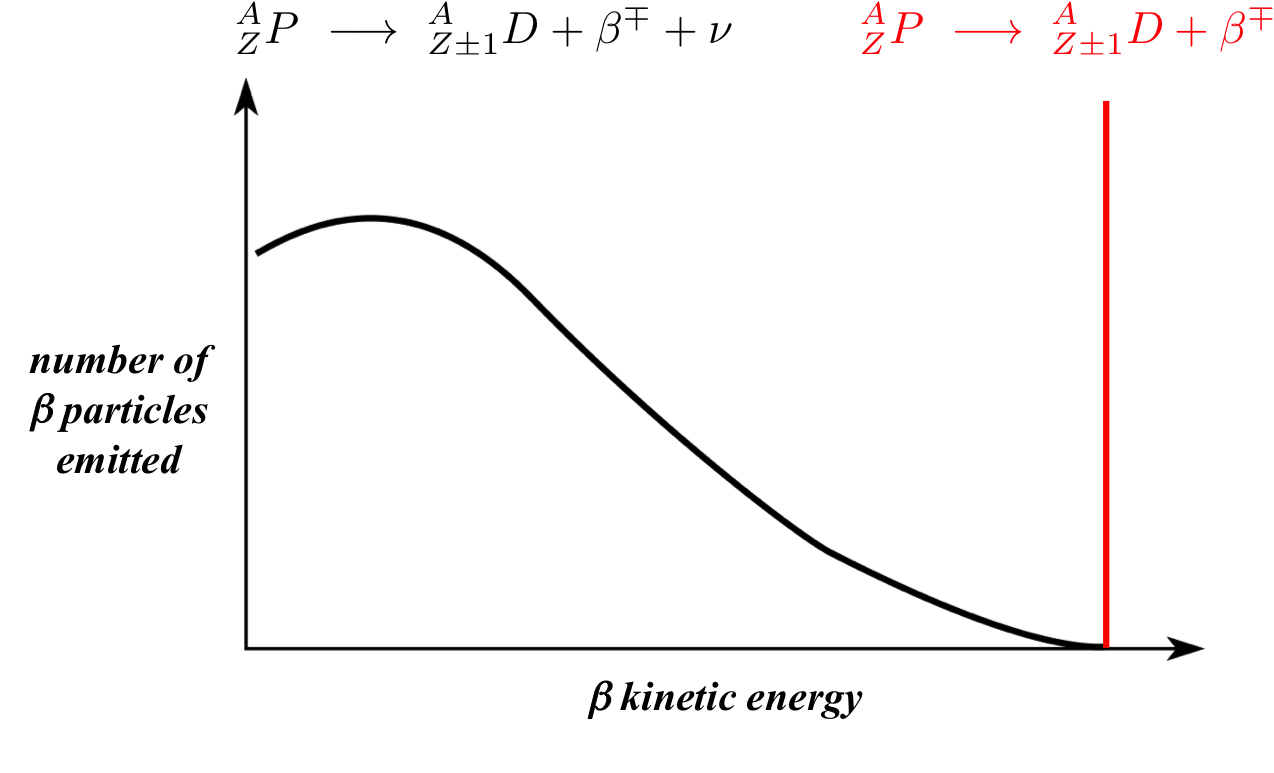
\includegraphics[width=0.75\columnwidth]{Neutrino/betaspectrum.png}
\caption{Kinetic energy distribution of the $\beta$ particle (electron or positron) produced in the decay of a parent nucleus $P$ into a daughter nucleus $D$. Units are arbitrary. Red curve: neutrinoless $\beta$ decay (Eq.~\ref{eq:beta_dirac}). The position of the quasi-Dirac spectrum is obtained by computing the reaction quotient. Black curve: continuous spectrum of $\beta$ decay involving a third particle (Eq.~\ref{eq:beta_cont}). Here, $\nu$ refers to an electron neutrino or antineutrino in the $\beta^{+}$ and $\beta^{-}$ decay respectively.}
\label{fig:betaspectrum}
\end{center}
\end{figure}

Two years following the discovery of the electron in 1897 by Sir Joseph John Thomson, Hernest Rutherford distinguished two types of radioactive emissions from some atomic nuclei: \textit{alpha} decay, where the nuclei emit $^{4}_2 \mathrm{He}^{2+}$; and \textit{beta} decay, in which the nuclei emit an electron\footnote{or a positron, differentiating between $\beta^{\mp}$ decays}. In 1914, however, it became apparent that an important ingredient was missing. In fact, if only a $\beta$ particle were released from the transmutation of a parent nucleus $P$ into a daughter nucleus $D$, \textit{i.e.}

\begin{equation}
\label{eq:beta_dirac}
\begin{array}{ccc}
^{A}_{Z}P & \longrightarrow & ^{A}_{Z\pm1}\mathrm{D}^{\pm} + \beta^{\mp}
\end{array}
\end{equation} \\ then the momentum spectrum of the beta particle would be a quasi-Dirac\footnote{because of Heisenberg's uncertainty principle, $\Delta E \Delta t \sim \hbar$, it would have some fundamental albeit tiny width due to the intrinsic uncertainty on the particle's energy} as illustrated by the red line in Fig.~\ref{fig:betaspectrum}. However, the momentum spectrum of the $\beta$ particles were instead continous, as per the black curve in  Fig.~\ref{fig:betaspectrum}. This suggests either that energy isn't conserved in $\beta$ decays or that the energy of the $\beta$ particle is shared by an additional unseen particle. This latter remedy, characterised as desperate at the time, was postulated by Wolfgang Pauli in 1930 in a famous letter\footnote{\url{http://www.physics.princeton.edu/~mcdonald/examples/EP/pauli_neutrino_30_english.pdf}} adressed to the community of \guillemotleft \textit{radioactive ladies and gentlemen} \guillemotright. He is often quoted saying to Niels Bohr: \\
\vspace{5pt}
\begin{center}
{\guillemotleft} ~I have done a terrible thing: I have postulated a particle that cannot be detected. ~ {\guillemotright} \\
\end{center}
\vspace{5pt}
Although many PhD students are often brought to make much more terrible assumptions, the existence of Pauli's undetectable particle was eventually inferred from weak interactions, the framework of which was developped by Enrico Fermi only 4 years later. In our current interpretation of $\beta$ decay, the transmutation of atomic nuclei is enabled by the emission or absorption of a $W^{\pm}$ gauge boson which mediates --- along with the $Z^0$ boson --- the weak interaction. These bosons are heavier than the nucleons they transmute which in turn make them, according to the Heisenberg uncertainty principle, very short-lived, with a half life of $\sim 3 \times 10^{-25}~s$. As such, this interaction is deemed short-ranged, hence coined \textit{weak} interaction. In the case of $\beta^{\mp}$ decay, the $W$ boson decays into an electron (or positron) and the additional particle, labelled $\nu$, such that
\begin{equation}
\label{eq:beta_cont}
\left\{
\begin{array}{lcl}
^{A}_{Z}P & \longrightarrow & ^{A}_{Z\pm1}\mathrm{D}^{\pm} + W^{\mp} \\
W^{\mp} & \longrightarrow & e^{\mp} + \nu
\end{array}
\right.
\end{equation} \\ whose properties were derived from Enrico Fermi's newly built theory of the weak interaction and dubbed the hypothetical particle the \textbf{neutrino} as it must be electrically neutral, and is very small\footnote{in the context of particle physics, small refers to its interaction cross section}. As it turns out, the particle involved in $\beta^{-}$ decay of neutrons is actually its conjugate anti-particle, the electron \textit{antineutrino}. Initially, neutrinos\footnote{technically speaking, neutrino borrowing of Italian vocabulary, the plural form should be \textbf{neutrini}. However, to prevent any confusion, I chose to use the anglocentric version, \textbf{neutrinos}} were thought to be massless and virtually undetectable. Nevertheless, neutrinos were discovered in 1956 when nuclear reactor synthesized antineutrinos by beta decay reacted with protons to produce neutrons and positrons \citep{nu_e_discovery}, a reaction known as \textit{electron capture} (see second expression in Eq.~\ref{eq:three_reactions}). The discovery is attributed to Clyde Cowan and Fredrick Reines who have been awarded the 1995 physics Nobel prize. In the following subsection, I summarize the neutrino's properties in the context of the standard model of particle physics.\\

\subsection{The Standard Model of Particle Physics}

\subsubsection{Neutral Leptons}

All fundamental particles are described by a set of quantum numbers, \textit{i.e.} degrees of freedom to fully determine their wave function. In addition to their principal ($n$), azimuthal ($\ell$) and magnetic ($m$) quantum numbers, the wave function of a fundamental particle requires the knowledge of its spin ($s$) which can either be an integer (bosons) or semi-integer (fermions) multiple of the Planck action $\hbar$. In the Standard Model (SM) of particle physics, fermions with $s/\hbar=1/2$ can be distinguished between two main types of particles: \\

\begin{itemize}
\item[$\bullet$] quarks, which are sensitive to all four fundamental interactions: strong, weak, electromagnetic and gravitational. They interact with one another via gluons, the carrier boson for the strong interaction. Due to color confinement, a property of the strong interaction, quarks cannot be observed directly in isolation, but rather through the composite particles they constitute:\\
\begin{itemize}
\item[$\star$] baryons, which have 3 valence quarks,\\
\item[$\star$] mesons, which are a combination of a quark and an antiquark. \\
\end{itemize}
These two can be distinguished by the computation of the baryon number $B = n_q - n_{\bar{q}}$ which is defined as the number of quarks (each having $n_q = 1/3$) minus the number of their conjugate anti-quarks ($n_q = -1/3$). As such, baryons have $B=1$ whereas mesons have $B=0$. There are 6 different quark flavours, \textit{a.k.a.} colours, arranged into 3 generations of hierarchical mass of a positively ($Q/e=2/3$) and a negatively ($Q/e=-1/3$) charged pair:\\
\begin{itemize}
\item[$\star$] first (light) generation: \textit{up} ($u$) and \textit{down} ($d$), \\
\item[$\star$] second (medium) generation: \textit{charm} ($c$) and \textit{strange} ($s$), \\
\item[$\star$] third (heavy) generation: \textit{top} ($t$) and \textit{bottom} ($b$). \\
\end{itemize}

\item[$\bullet$] leptons, which are not sensitive to the strong interaction, and, in the case of neutrinos, the electromagnetic interaction. There are 6 different leptons, arranged into 3 generations of hierarchical mass\footnote{this is not necessarily the case for the neutrinos} of a negatively charged ($Q/e=-1$) and electrically neutral pair: \\
\begin{itemize}
\item[$\star$] first (electronic) generation: $e$ and $\nu_e$, \\
\item[$\star$] second (muonic) generation: $\mu$ and $\nu_\mu$, \\
\item[$\star$] third (tauic) generation: $\tau$ and $\nu_\tau$, \\
\end{itemize}
Leptons are characterized by a lepton number, which is $L=1$ for any lepton and $L=-1$ for any anti-lepton. \\
\end{itemize}

\subsubsection{The Weak Interaction}

\begin{figure}
\begin{center}
%
\includegraphics[width=0.35\columnwidth]{Neutrino/bcci.png}
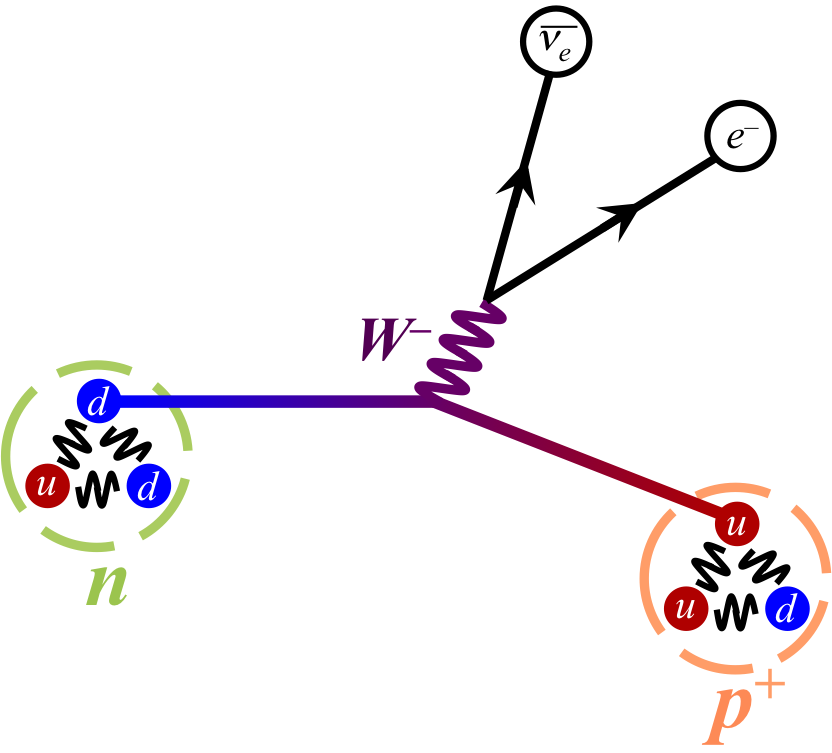
\includegraphics[width=0.5\columnwidth]{Neutrino/ntop.png}
\caption{Schematic space-time diagram representation of the weak interaction involved in the $\beta^{-}$ decay. Time flows from left to right. The sinusoidal lines are bosons: gluons in black, confining the quarks via the strong interaction; and the $W$ boson in purple. $p^{+}$ refers to a proton $^{1}_{1}\mathrm{H}^{+}$}
\label{fig:weakcurrent}
\end{center}
\end{figure}

In laymen terms, the weak force is the interaction involved whenever a quark alters its flavour. In Fig.~\ref{fig:weakcurrent}, one of the neutron's valence quarks' flavour switches from down (in blue) to up (in red) --- transmutting the composite particle from a neutron to a proton in the process --- the cost of which is the emission of a charged (here negatively charged) $W$ boson. The latter is short-lived and decays into an electron and an electron-flavoured antineutrino. The Feynman diagram in Fig.~\ref{fig:weakcurrent} illustrates the $\beta^{-}$ decay reaction described in Eq.~\ref{eq:beta_cont}. By reversing the charge, parity or time operators of one or several of the products or reactants involved, this Feynman diagram can also describe the electron capture and inverse $\beta$ decay:

\begin{equation}
\label{eq:three_reactions}
\left\{  
\begin{array}{rl}
^{1}_{0}n &\longrightarrow ^{1}_{1}\mathrm{H}^{+} + e^{-} + \bar{\nu}_e \\
e^{-} + ^{1}_{1}\mathrm{H}^{+} &\longrightarrow ^{1}_{0}n + \nu_e \\
\bar{\nu}_e + ^{1}_{1}\mathrm{H}^{+} &\longrightarrow ^{1}_{0}n + e^{+}
\end{array}
\right.
\end{equation}

In all cases, this basic description of the charged current weak interaction illustrates how a generic quark interacts non-elactically with a generic lepton.

\subsubsection{Lepton Flavours}

Neutrinos and antineutrinos can be produced by both the $W^{\pm}$ and $Z^0$ bosons:
\begin{equation}
\begin{array}{lcccr}
W^{+} \longrightarrow e^{+} + \nu_e & ~~~~~ & W^{-} \longrightarrow e^{-} + \bar{\nu}_e & ~~~~~ & Z \longrightarrow \nu_e + \bar{\nu}_e \\
\\
W^{+} \longrightarrow \mu^{+} + \nu_\mu & ~~~~~ & W^{-} \longrightarrow \mu^{-} + \bar{\nu}_\mu & ~~~~~ & Z \longrightarrow \nu_\mu + \bar{\nu}_\mu \\
\\
W^{+} \longrightarrow \tau^{+} + \nu_\tau & ~~~~~ & W^{-} \longrightarrow \tau^{-} + \bar{\nu}_\tau & ~~~~~ & Z \longrightarrow \nu_\tau + \bar{\nu}_\tau
\end{array}
\end{equation} \\ A neutrino's or antineutrino's lepton flavour is defined as that of the charged lepton with which it is interacting. The $W$ bosons can also decay into a quark anti-quark pair $q\bar{q}$. The $W$ decay channels are summarized in Fig.~\ref{fig:Wdecay}. Its decay width, of $\Delta m_W = 2.085 \pm 0.042~\mathrm{GeV}/c^2$ \citep{W_decay_width}, is proportional to the summed probability of all the possible aforementioned decay channels, and is consistent with $3$ lepton charges, hence a total of $3$ generations of leptons, either charged or neutral. In other words, if a fourth neutrino were to be discovered, it wouldn't have a lepton charge as it wouldn't interact with the $W$ bosons, hence making it insensitive to the weak interaction. \\

The particle discovered by Cowan, Reines and their collaborators is the electron flavoured antineutrino. In the early 1940s, an additional neutrino particle was hypothesized: the \textbf{neutretto}, which later became commonly known as the muon flavoured neutrino. It was discovered in 1962 by Leon Max Lederman, Melvin Schwartz and Jack Steinberger \citep{nu_mu_discovery}, who were awarded the 1988 physics Nobel prize. The third neutrino lepton flavor was hypothesized upon the discovery of the tau ($\tau^{-}$) lepton in a series of experiments at the Stanford Linear Accelerator Center (SLAC-LBL) from 1974 to 1977 \citep{tau_discovery}. The tau neutrino was discovered in 2000 by the Direct Observation of the Nu Tau (DONUT) collaboration \citep{nu_tau_discovery} at Chicago's Fermilab. \\

\begin{figure}
\begin{center}

\includegraphics[width=0.5\columnwidth]{Neutrino/Wdecay.png}
\caption{\textbf{Left:} $W$ decay into a lepton pair (charged and neutral) $\ell \in \lbrace e, \mu, \tau \rbrace$. \textbf{Right:} $W$ decay into a quark anti-quark pair.}
\label{fig:Wdecay}
\end{center}
\end{figure}


\subsubsection{Helicity}


All particles have angular momentum, which for those described by quantum mechanics\footnote{quantum mechanics is often erroneously described as the theory which descibes small systems. What is implied by small is the characteristic length of the system. However, quantum mechanics can apply to large systems such as neutron stars, and can not apply to small systems such as a handful of gas molecules. In more exact terms, quantum mechanics applies to systems whose \textbf{action} is comparable to the Planck constant.} is the vector sum of its orbital momentum and its spin $\vec{j} = \vec{\ell} + \vec{s}$. Since the orbital momentum is orthogonal to the plane formed from the position and linear momentum, $\vec{\ell} = \vec{r} \times \vec{p}$, its component along $\vec{p}$ is zero. Helicity, defined as the projection of spin onto the direction of linear momentum,

\begin{equation}
\hat{h} = \vec{s} \cdot \frac{\vec{p}}{\vert \vert \vec{p} \vert \vert}
\end{equation} \\ is a conserved quantity. Since the spin's eigenvalues are discrete along an axis, so are those of the particle's helicity, which are $[\![ -s, +s ]\!]$ with $s$ the spin of the particle. As such, fermions with $s/\hbar=1/2$ can have $\pm 1$ helicity. Particles having positive (\textit{resp.} negative) helicity, \textit{i.e.} whose spin is aligned (\textit{resp.} opposed) to its linear momentum, are commonly refered to as being \textbf{right-handed} (\textit{resp.} \textbf{left-handed}). The choice of this nomenclature is motivated by the schematic in Fig.~\ref{fig:helicity}. \\
 
\begin{figure}
\begin{center}
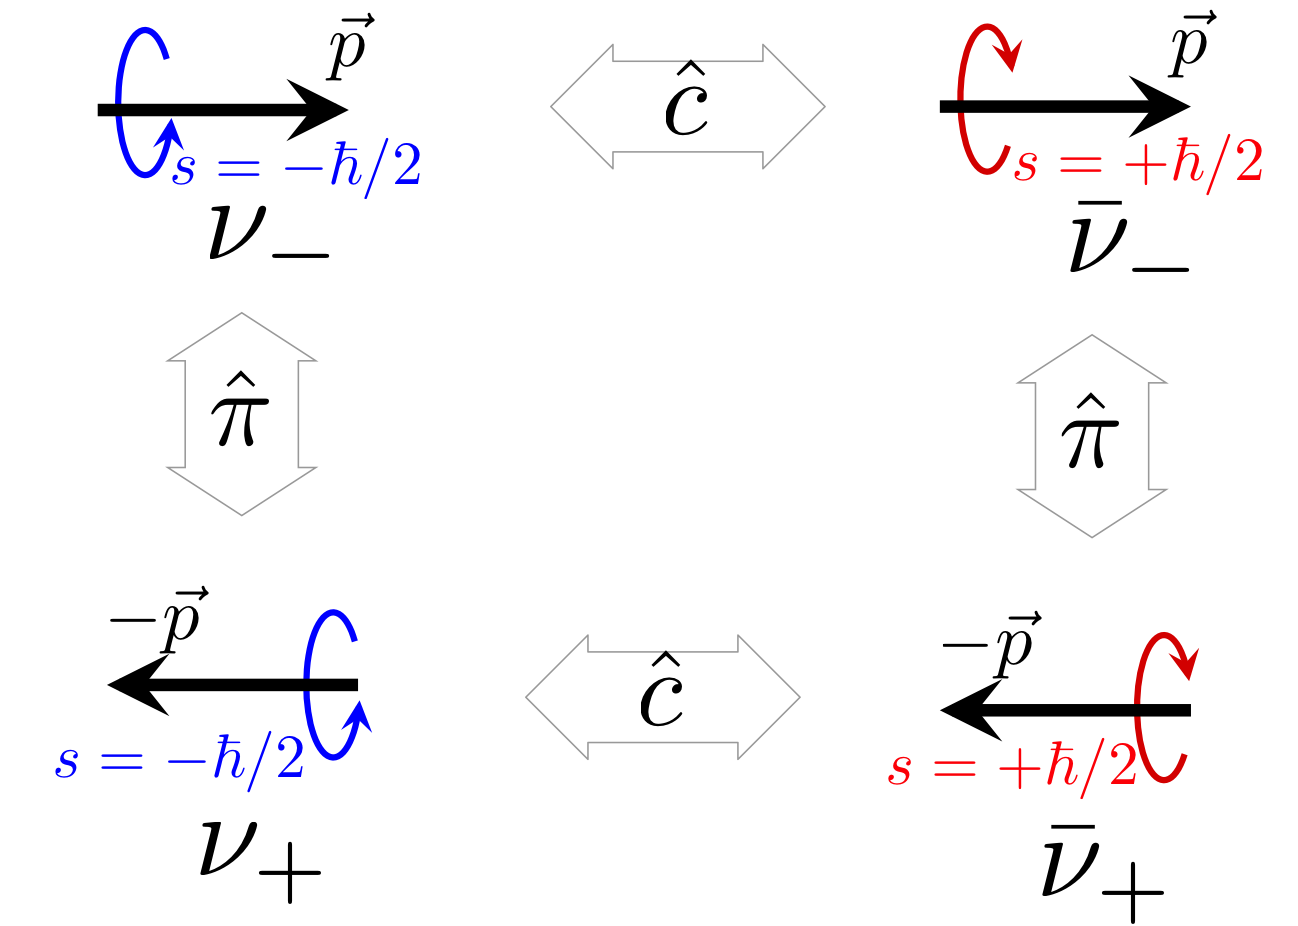
\includegraphics[width=0.75\columnwidth]{Neutrino/helicity.png}
\caption{Clockwise from top left: Left-handed neutrino, left-handed antineutrino, right-handed antineutrino and right-handed neutrino. The black arrows depict the particle's linear momentum. Its direction is inversed by the parity operator $\hat{\pi}$ applied from top to bottom row. The red and blue arrows depict the particle's spin. Its sign is inversed by the charge conjugation operator $\hat{c}$, applied from left to right columns. The $\pm$ subscipts denote the sign of the particle's helicity. The right or left handedness illustrates how the arrows materializing the spin of the particles wrap around the pointing direction of $\vec{p}$, as one's fingers wrap around the thumb. So far, only the negative helicity neutrino (top left) and positive helicity antineutrino (bottom right) are observed states in nature and predicted by the SM. The remaining two states are hypothetical and introduced in the $\nu$MSM in Sec.~\ref{sec:numsms}.}
\label{fig:helicity}
\end{center}
\end{figure}

A particle's linear momentum is relative to a reference frame, while its spin is invariant. Therefore, the particle's helicity, like its linear momentum, depends on the reference frame. Two observers, one moving slower and the other faster than a moving electron will disagree on the direction of its linear momentum with respect to their reference frame, and thus disagree on the electron's helicity sign. \\

In the SM, neutrinos are massless and therefore travel at the speed of light. As a consequence, there are no observers capable of travelling faster than the neutrino, hence only one of the two helicity signs is observed. Neutrinos appear to have intrinsically left-hand helicity. In the SM, the only right-handed neutral leptons are anti-neutrinos. Consequently, the weak interaction involving neutrinos or anti-neutrinos violates conservation of parity\footnote{the parity operator $\hat{\pi}$ mirrors the coordinates of a wavefunction, \textit{i.e.} $\hat{\pi} \left\vert \psi (\vec{r}) \right\rangle = \left\vert \psi (-\vec{r}) \right\rangle$}.  \\




\subsection{Why Neutrinos Are Interesting}

Neutrinos, despite completing our understanding of $\beta$ decay and other weak processes, are of particular interest in particle physics as they hint at the incompleteness of the Standard Model. The question whether neutrinos are a Dirac or Majorana particle remains to this day unanswered. If the latter is correct, which is plausible since they are electrically neutral, then that could resolve the issue of their left-handedness. If such is the case, then one would expect to observe neutrinoless $\beta$ decay processes, which haven't been confirmed as of today. \\

An antiparticle's wave function is the conjugate of its corresponding particle. In terms of the charge conjugation operator $\hat{c}$, $\left\vert \bar{\psi} \right\rangle = \hat{c} \left\vert \psi \right\rangle$. If this identity is applied to a neutrino, then its conjugate antineutrino would have the same helicity state. Since the left-handed  antineutrino state is currently unobserved in nature, one needs to apply the parity operator to the antineutrino's wave function, which reverse the linear momentum direction but conserves spin orientation, thereby reversing the helicity (see Fig.~\ref{fig:helicity}):

\begin{empheq}[box=\mymath]{equation}
\left\vert \bar{\nu} \right\rangle = \hat{c} \hat{\pi} \left\vert \nu \right\rangle
\end{empheq} \\ Although weak interactions don't conserve parity, its Hamiltonien $\hat{\mathcal{H}}$ commutes with $\hat{c}\hat{\pi}$ --- also called CP symmetry preservation --- since it is \textit{a priori} an invariant under this transformation. As recently as early August 2017, the Tokai to Kamioka (T2K) experiment has announced hints of a possible CP violation by neutrinos\footnote{\url{http://t2k-experiment.org/2017/08/t2k-2017-cpv/}}. If neutrinos indeed violate CP symmetry, they could provide a plausible explanation for the lepton (and baryon) asymmetry in the Universe. \\



On the astrophysical side, if detected in large enough quantities, they can serve as an alternative messenger from photons. The short range of their interaction with matter enable them to travel through dense zones unimpeded, but they also make their detection all the more challenging. This double-edged sword can nevertheless be useful in probing the Sun's core or the central zone of a supernova explosion, which produce massive quantities of neutrinos.\\


Provided neutrinos have non-zero mass, they could also constitute a candidate particle for dark matter. 
%\subsection{The Standard Model of Particle Physics}

%\subsection{Discovery of Neutrinos}

%\subsection{Neutrinos' Properties}

\clearpage

	\section{Neutrino Masses: Beyond the Standard Model}
	\label{sec:bsm}
	The properties of neutrinos summarized in the previous section pertain to those derived from the standard model. However, the latter is incomplete in its description of neutrino mass. In this section, I explain how we know neutrinos have non-zero mass and how cosmological probes can assist particle physics in determining the sum of their mass eigenstates.

\subsection{Lepton Flavour Oscillations}
\label{sec:leptonmix}


A notable counter-intuitive property\footnote{oscillations are not inherent to neutrinos; in fact, there is a misalignment between the propagating quantum states of quarks and when they partake in strong interactions.} of neutrinos is their capacity to alter their lepton charge. Predicted in 1957 by \cite{Pontecorvo57, Pontecorvo58}, the first experiment that detected these neutrino flavour oscillations can be traced back to the 1968 Homestake experiment, in which, using a chlorine-based detector, \cite{Davis68} reported a deficit in the flux of solar neutrinos with respect to the SM prediction. This deficit became known as the solar neutrino problem. Accounting for this solar deficit by flavour oscillations was made definitive in 2001 at the Sudbury Neutrino Observatory (SNO) in Ontario \citep{Sudbury_osc}. Three years prior, the Super-Kamiokande scintillator based in Japan had gathered evidence for the oscillation of flavours in atmospheric neutrinos \citep{Fukuda1998, Kajita1999}. As such, the 2015 physics Nobel prize was attributed to both Takaaki Kajita and Arthur B. McDonald for not only the detection of neutrino flavour oscillations but also evidence for non-zero neutrino masses. Indeed, if neutrinos were massless as is predicted by the SM, then, like photons, they would propagate at the speed of light and experience infinite time dilation\footnote{since their Lorentz factor $\gamma = (1-(v/c)^2)^{-1/2} \rightarrow \infty$}. Since neutrino lepton flavours oscillate, their time dilation cannot be infinite, and they therefore cannot travel at the speed of light, which means at least one neutrino eigenstate must have non-zero mass. \\

To make sense of this rather odd phenomenon, it is useful to regard the lepton charge of the neutrino as nothing more than that of the charged lepton with which it interacts via the weak force. The wave function that propagates through space in time is a time-dependent quantum superposition of \textit{mass} eigenstates $m_i = m_{1,2,3}$. When interacting, the lepton states $\nu_\ell = \nu_{e, \mu, \tau}$ are fixed superposition of those mass eigenstates:

\begin{empheq}[box=\mymath]{equation}
\displaystyle
\left\vert \nu_\ell \right\rangle = \sum\limits_{i} U^{\dagger}_{\ell i} \left\vert \nu_i \right\rangle
\end{empheq}

There is no trivial reason why these mass eigenstates should be aligned with the lepton (observed) states. In other words, the mass-flavour mixing matrix $U$, \textit{a.k.a.} the Pontecorvo–Maki–Nakagawa–Sakata (PMNS), is not diagonal. Since there are three possible lepton charges, as justified by the decay width of the $W$ boson, it is natural although arbitrary to expect three different mass eigenstates. If at least one of the eigenstates is different than the other two, then the superposition would propagate at different rates and lepton flavors are expected to oscillate.\\

\begin{figure}
\begin{center}
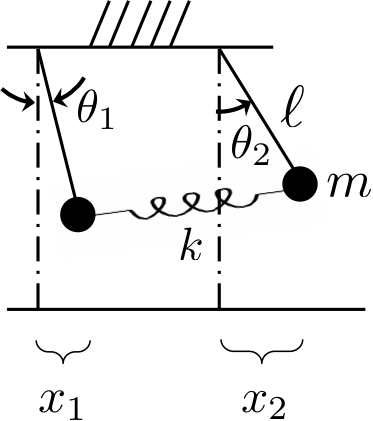
\includegraphics[width=0.25\columnwidth]{Neutrino/coupled_pendula.png}
\caption{Setup of the coupled pendula, marked by $x_1$ and $x_2$.}
\label{fig:pendulum}
\end{center}
\end{figure}

To illustrate why, it can be useful to consider the coupled pendula in Fig.~\ref{fig:pendulum}. The positions $x_1$ ad $x_2$ of the similar masses $m$ hanging in a constant gravitational field $g$ from identical lengths $\ell$ and linked by a spring of stiffness $k$ from their equilibrium positions, obey \\
\begin{equation}
\left( 
\begin{matrix}
\cfrac{d^2}{dt^2} + \cfrac{g}{\ell} + \cfrac{k}{m} & - \cfrac{k}{m} \\
- \cfrac{k}{m} & \cfrac{d^2}{dt^2} + \cfrac{g}{\ell} + \cfrac{k}{m}
\end{matrix}
\right)
\left( 
\begin{matrix}
x_1 \\
\\
x_2
\end{matrix}
\right) = \left( 
\begin{matrix}
0 \\
\\
0
\end{matrix}
\right)
\end{equation} \\ The coupled pendula system admits 2 normal modes, depicted in Fig.~\ref{fig:normal_mode}, which satisfy the eigenvalue equation, \\

\begin{equation}
x_{\pm} = x_2 \pm x_1 = a_{\pm} \cos \left( \omega_{\pm} t + \phi_{\pm} \right)
\end{equation} \\ where $\omega_{+}^2 = g / \ell$ and $\omega_{-}^2 = \omega_{+}^2 + 2 k / m$. The presence of the spring makes the natural frequency of the inverse mode, in which the masses oscillate with opposite directions, higher than that of the normal mode, in which the masses swing in unison: $\omega_{-} > \omega_{+}$. The generic solution is a superposition of both of these modes:

\begin{equation}
\label{eq:genericsol}
\left(  
\begin{matrix}
x_1 \\
x_2
\end{matrix}
\right) = \left(
\begin{matrix}
1 & 1\\
1 & -1
\end{matrix}
\right) \left(
\begin{matrix}
x_{+}\\
x_{-}
\end{matrix}
\right)
\end{equation}

\begin{figure}
\begin{center}
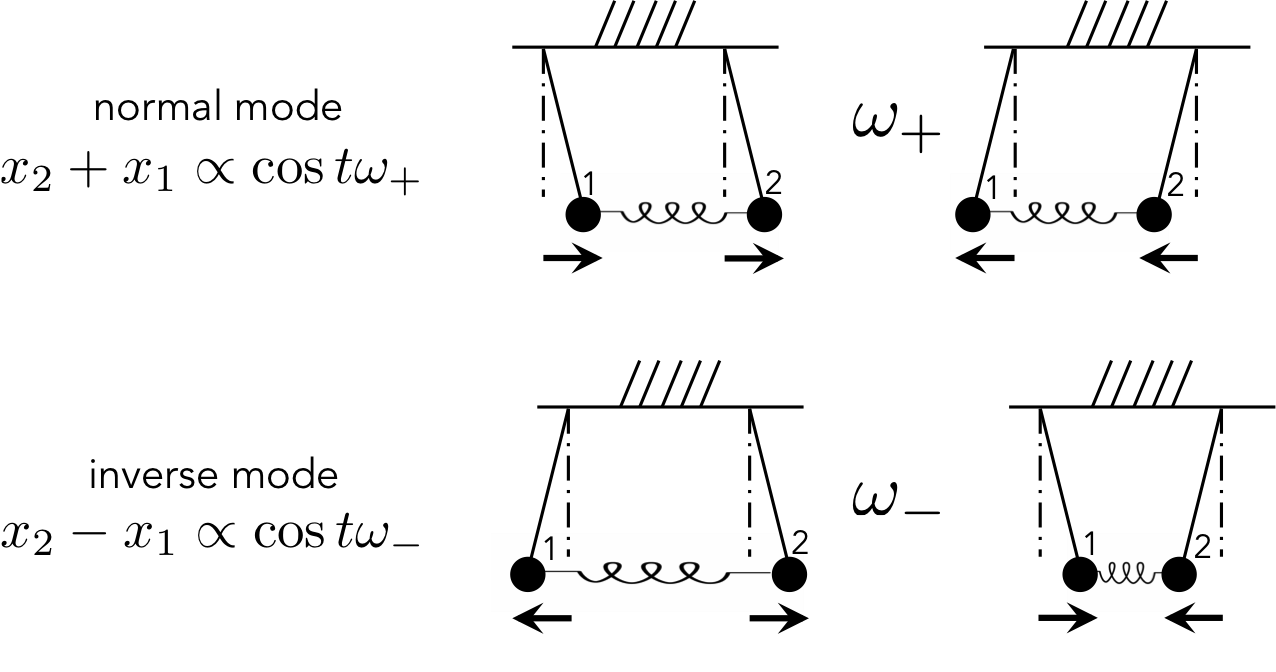
\includegraphics[width=0.85\columnwidth]{Neutrino/normal_modes.png}
\caption{The two normal modes of the coupled pendula, oscillating at frequencies $\omega_{\mp}$.}
\label{fig:normal_mode}
\end{center}
\end{figure}

Because the two modes oscillate at different frequencies, nudging the left pendulum only from its equilibrium position will inevitably result in the right pendulum swinging. The less stiff the spring or the heavier the masses, the more time the left pendulum will swing leaving the right one relatively unperturbed. After several cycles, the left pendulum's oscillations will dampen to a halt, with all the initial momentum transfered to the right one ! The oscillations of both pendula are plotted on Fig.~\ref{fig:trajectory_pendulum}. \\

\begin{figure}
\begin{center}
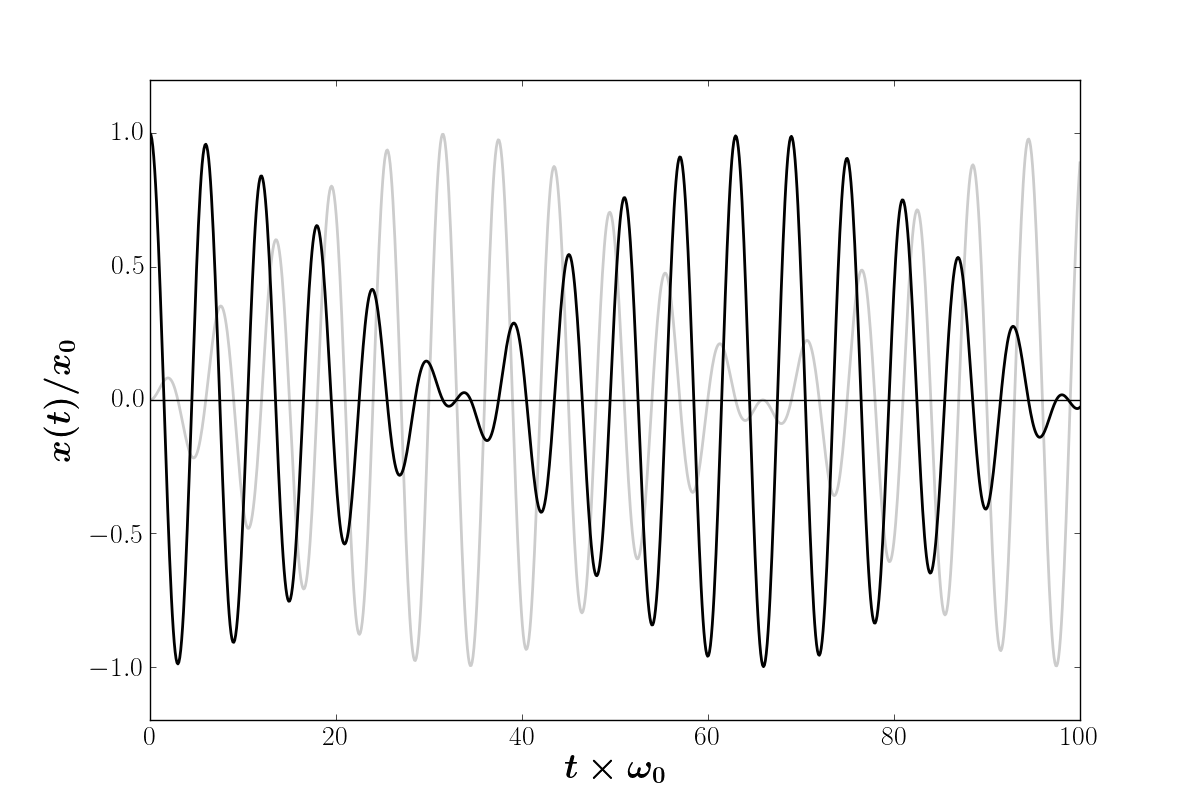
\includegraphics[width=0.85\columnwidth]{Neutrino/pendulum_x.png}
\caption{Position of the two pendula from their respective rest postitions, as a function of time. Black curve: $x_1$. Grey curve: $x_2$.}
\label{fig:trajectory_pendulum}
\end{center}
\end{figure}


\subsection{Neutrino Masses and Mixing}
\label{sec:numassmix}

\begin{figure}
\begin{center}
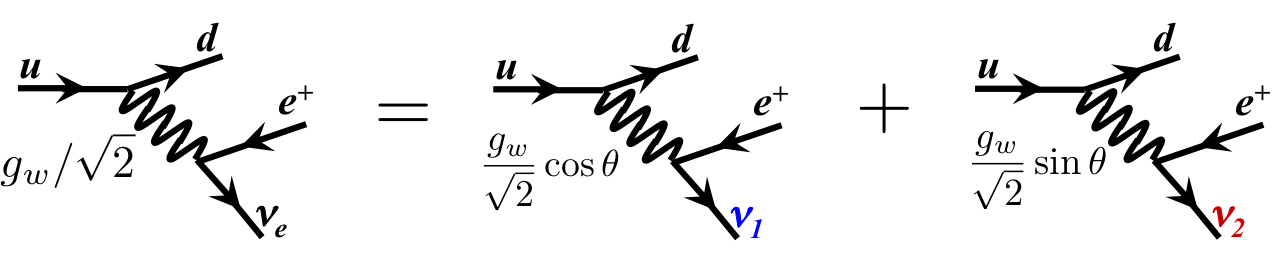
\includegraphics[width=0.9\columnwidth]{Neutrino/seesaw.png}
\caption{Feynman diagram of $\beta^{+}$ decay, producing an electron-flavoured neutrino, which can be interpreted as the superposition of two normal modes (here two mass eigenstates).}
\label{fig:mixing}
\end{center}
\end{figure}

This simple coupled pendula is analogous to neutrino flavour oscillations involving $2$ observation states $\ell = \lbrace e, \mu \rbrace$ and $2$ mass eigenstates $i = \lbrace 1, 2 \rbrace$. As Fig.~\ref{fig:mixing} illustrates, the electron neutrino produced in $\beta^{+}$ decay for instance can be described in mathematical terms as the superposition of the production of eigenstates $\nu_1$ and $\nu_2$. If one notes $\theta$ as the mixing angle between the two mass eigenstates, then 

\begin{equation}
\label{eq:2eigen}
\left( 
\begin{array}{c}
\nu_e \\
\nu_\mu \\
\end{array}
\right) = \left(
\begin{array}{cc}
c_{12} & - s_{12} \\
s_{12} & c_{12}
\end{array}
\right)
\left( 
\begin{array}{c}
\nu_1 \\
\nu_2 \\
\end{array}
\right)
\end{equation} \\ where $c_{12} \doteq \cos \theta$, $s_{12} \doteq \sin \theta$. Since $\cos^2 \theta + \sin^2 \theta = 1$, $c_{12}$ and $s_{12}$ can be interpreted as the interaction probability with each of the eigenstates. Notice the similarity of Eq.~\ref{eq:2eigen} and Eq.~\ref{eq:genericsol}. Each of these eigenstates is a normal mode of the coupled pendula, while the lepton states correspond to the $(x_1 = x_{\mathrm{max}}, x_2=0)$ and $(x_1 = 0, x_2 = x_{\mathrm{max}})$ configurations. Since $\theta \neq 0$, the eigenstates are misaligned and as time elapses, they propagate in space at different rates. At any given time, the probability of measuring flavour $\ell$ is given by the quantity

\begin{equation}
\label{eq:oscprob}
\left\vert \left\langle \nu_\ell \vert \nu (t) \right\rangle \right\vert^2 =  \sin^2 \left( 2 \theta \right) \times \sin^2 \left( \frac{L \Delta m^2}{4 E} \right)
\end{equation} \\ where $E$ is the energy of the eigenstate, $L$ is the distance travelled from the source, assuming it is produced in the other state than the one measured, and $\Delta m^2 = \vert m^2_2 - m^2_1 \vert$. The probability of detecting flavour $\ell$ as a function of $L/E$ can be visualized by squaring the curve in Fig.~\ref{fig:trajectory_pendulum}, in which one can distinguish two characteristic frequencies. The first right-hand term of Eq.~\ref{eq:oscprob}, \textit{i.e.} the intrinsic misalignment of the mass eigenstates, predominates the short-range oscillations; whereas the long-range oscillations forming the envelope are governed by the right-most term, and is determined by the distance from source to target. \\



Since there are three lepton charges, and at least as much mass eigenstates, then a more fitting classical analog would be three pendula coupled to each other with three (not two!) springs. Similar to Eq.~\ref{eq:2eigen}, the $3$ mass eigenstates are related to the lepton states via a $3 \times 3$ mass PMNS mixing matrix, \\


\begin{equation}
\left( 
\begin{array}{c}
\nu_1 \\
\nu_2 \\
\nu_3
\end{array}
\right) = 
U_1 U_2 U_3 \Delta
\left( 
\begin{array}{c}
\nu_e \\
\nu_\mu \\
\nu_\tau
\end{array}
\right)
\end{equation} \\ It can be decomposed into the $3$ rotation matrices between eigenstates $\nu_i$ and $\nu_j$, 

\begin{equation}
U_1 = 
\left( 
\begin{array}{ccc}
1 & 0 & 0 \\
0 & c_{23} & s_{23} \\
0 & -s_{23} & c_{23}
\end{array}
\right)~~~~~
U_2 = 
\left( 
\begin{array}{ccc}
c_{13} & 0 & s_{13}e^{i \delta} \\
0 & 1 & 0 \\
- s_{13}e^{i \delta} & 0 & c_{13}
\end{array}
\right)~~~~~
U_3 = 
\left( 
\begin{array}{ccc}
c_{12} & s_{12} & 0 \\
- s_{12} & c_{12} & 0 \\
0 & 0 & 1
\end{array}
\right)
\end{equation} \\ and a phase matrix

\begin{equation}
\Delta = 
\left( 
\begin{array}{ccc}
e^{i \alpha_1 / 2} & 0 & 0 \\
0 & e^{i \alpha_2 / 2} & 0 \\
0 & 0 & 1
\end{array}
\right)
\end{equation} \\ which yields a total of 9 neutrino parameters: \\

\begin{itemize}
\item[$\bullet$] the mixing angles $\theta_{12}$, $\theta_{13}$ and $\theta_{23}$;
\item[$\bullet$] the (squared) mass differences $\Delta m^2_{21}$, $\Delta m^2_{31}$ and $\Delta m^2_{32}$; and
\item[$\bullet$] three phases $\alpha_1$, $\alpha_2$ and $\delta$.\\
\end{itemize} 
For a $n \times n$ mixing matrix, involving $n$ detectable states and $n$ mass eigenstates\footnote{$n=4$ (\textit{resp.} $n=6$) for adding 1 (\textit{resp.} 3) sterile neutrinos in addition to the left-handed states; see Sec.~\ref{sec:numsms} for motivation}, there are $n^2$ real parameters, including $n(n-1)/2$ angles and $n(n+1)/2$ phases. Not all of the phases are physical, however. So far, for the SM $n=3$ case, neutrino experients typically probe composites of these parameters, which are grouped in Tab.~\ref{tab:neutrinoparamexp}. Only $\delta$, $\alpha_{1,2}$ and the sign of $\Delta m^2_{32}$ remain unknown (see Sec.~\ref{sec:massorder}). \\


\subsection{Mass Ordering}
\label{sec:massorder}

\begin{table}
	\begin{center}
		\begin{tabular}{ccl}
			\toprule
			\textbf{parameter} & \textbf{constraint} & \textbf{experiment type} \\
			\midrule
			$\sin^2 2 \theta_{12}$ & $0.846 \pm 0.021$ & Solar: KamLand. Acc: Minos, T2K\\
			$\sin^2 2 \theta_{13}$ & $0.093 \pm 0.008$ & Reactor: Daya-Bay, RENO, D-Chooz. Acc: Minos, T2K\\
			$\sin^2 2 \theta_{23}$ & $\geqslant 0.92$ & Acc: Minos, T2K. Atmospheric \\
			$\Delta m^2_{\mathrm{sol}}$ & $(7.53 \pm 0.18) \times 10^{-5}~\mathrm{eV}^2$ & Solar: KamLAND \\
			$\Delta m^2_{\mathrm{atm}}$ & $(2.44 \pm 0.06) \times 10^{-3}~\mathrm{eV}^2$ & Atmospheric \\
			\bottomrule
		\end{tabular}
	\end{center}
	\caption{Current constraints on neutrino parameters. Quoted uncertainties are $1 \sigma$ when around a best fit value, and $90\%$ likelihood when lower bound. $\Delta m^2_{\mathrm{sol}} = \Delta m^2_{21}$ and $\Delta m^2_{\mathrm{atm}} = \vert \Delta m^2_{32} \vert \simeq \vert \Delta m^2_{31} \vert$. From \cite{PDG} and \cite{W_decay_width}.}
	\label{tab:neutrinoparamexp}
\end{table}

Although neutrino flavour oscillations involve $3$ mass eigenstates and $3$ lepton measured states, the measurement probability for the $n=2$ case in Eq.~\ref{eq:oscprob} can be used as an approximation to the oscillations between $\nu_{\mu} \longleftrightarrow \nu_{\tau}$ in atmosphere neutrinos, since $\nu_e$ are seldom involved. It also approximates solar neutrino oscillations, in which $\nu_e$ oscillate into a superposition of $\nu_\mu$ and $\nu_\tau$. These approximations are valid since $\theta_{13} \ll 1$ (see Tab.~\ref{tab:neutrinoparamexp}) and because two of the eigenstates are similar in mass relative to the remaining third one. \\

By convention, the mass eigenstates are labelled such that $\vert U_{e1} \vert^2 \geqslant \vert U_{e2} \vert^2 \geqslant \vert U_{e3} \vert^2$, implying that the $\nu_1$, $\nu_2$ and $\nu_3$ have decreasing components of $\nu_e$ in that order. With such convention, the solar neutrino oscillations are governed by $\Delta m^2_{21}$, as $\nu_{1,2}$ are `` electron-rich ''; whereas the atmospheric neutrino oscillations are governed by the other two squared mass difference. \cite{Sudbury_osc} established in the SNO experiment that $\Delta m^2_{21} > 0$. However, it is still unclear today whether $m^2_3 > m^2_2$ or $m^2_3 < m^2_1$, each case being known as the normal and inverted ordering respectively, illustrated in Fig.~\ref{fig:hier}. To determine the absolute scale of neutrino masses, one can go about two ways: measure either\\

\begin{itemize}
\item[$\bullet$] the lightest mass state, which can be deduced from an effective mass $m^2_\beta = \displaystyle\sum_{i=1}^{3} U_{e i} m^2_i$ probed by the products of $\beta$ decay from tritium $^3_1 \mathrm{H}$, attempted by experiments such as KATRIN \citep{KATRIN}; or\\

\item[$\bullet$] the sum of all three eigenstates $\sum m_\nu = m_1 + m_2 + m_3$, which is attempted by cosmological probes such as the Cosmic Microwave Background or, as is the case in this work, the Lyman-alpha forest.
\end{itemize}

\begin{figure}
\begin{center}
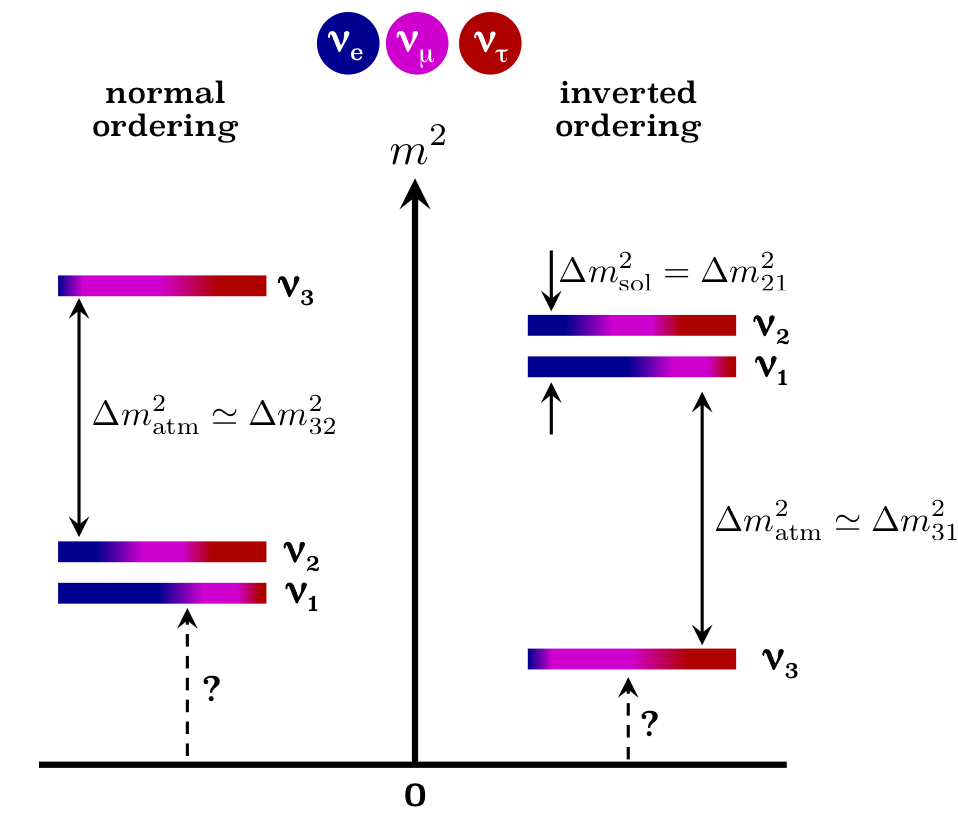
\includegraphics[width=0.6\columnwidth]{Neutrino/hierarchy.png}
\caption{Normal (left) and inverted (right) neutrino mass ordering. Blue, purple and red correspond to the $\nu_{e, \mu, \tau}$ lepton states and their proportion in the mass eigenstates reflect the PMNS matrix elements.}
\label{fig:hier}
\end{center}
\end{figure}


\clearpage

	\section{The Minimal Extension with Sterile Neutrinos}
	\label{sec:numsms}
	\subsection{Right-Handed Neutrinos}

Neutrinos having non-zero mass suggests the need of a finer physical description, or extension of the SM. Non-zero mass enables the existence of right-handed neutrinos and left-handed anti-neutrinos, since they do not move at the speed of light. Yet all neutrinos have been observed with left-handed and all anti-neutrinos right-handed chirality --- a relativistic invariant of any particle. A key unanswered question in particle physics is: can neutrinos and anti-neutrinos be differentiated just by their chirality, or do right-handed neutrinos and left-handed anti-neutrinos exist as separate particles? \\

\subsection{The $\nu$MSM}


One possible extension to the Standard Model is the addition of $3$ right-handed neutrinos. Dubbed the $\nu$MSM, it was originally proposed by \cite{nuMSM_1, nuMSM_2}. Such right-handed neutrinos would have no electric charge, no lepton charge, and no color, making them insensitive to all fundamental interactions aside from gravity, making them particularily challenging to detect. As such, they are often refered to as \textbf{sterile neutrinos} ($\nu_s = \nu_{\textsc{i}, \textsc{ii}, \textsc{iii}}$) to distinguish them from their left-handed lepton-flavoured counterparts ($\nu_\ell = \nu_{e, \mu, \tau}$). Fig.~\ref{fig:numsm} recaps these additions to the SM picture. \\

\begin{figure}[h]
\begin{center}
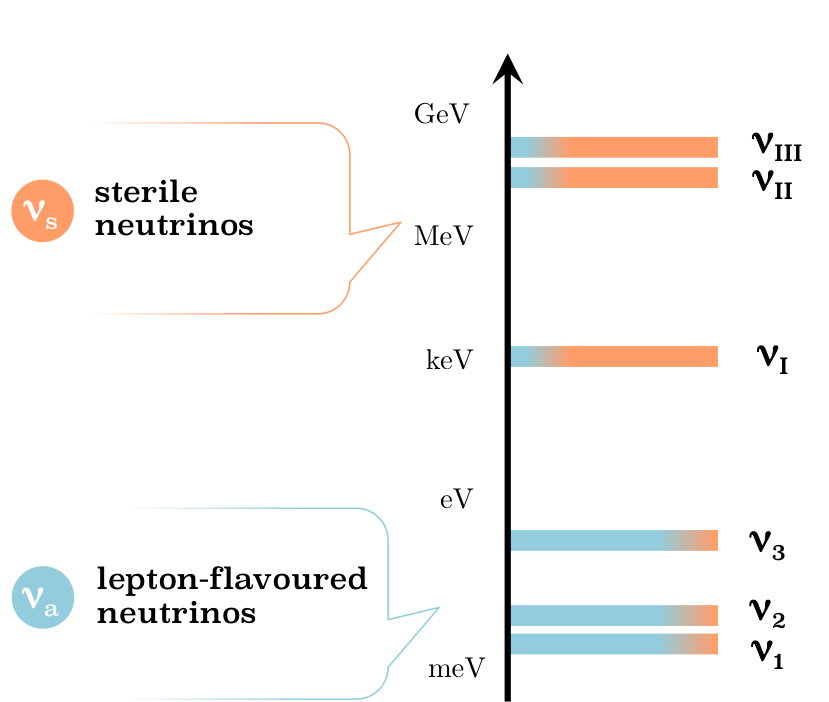
\includegraphics[width=0.5\columnwidth]{Neutrino/activesterile.png}
\caption{Assuming there are $3$ additional mass eigenstates $\nu_{\textsc{i}, \textsc{ii}, \textsc{iii}}$ such that $m_{\textsc{i}, \textsc{ii}, \textsc{iii}} \gg m_{1,2,3}$, and the angle between these heavier and lighter states is small, then the lepton-flavoured left-handed neutrinos of the SM can be thought of as a mixture of preponderantly the lighter eigenstatestates; whereas the $3$ remaining neutrinos are predominantly of the heavier eigenstates, carry no lepton flavour and are right-handed.}
\label{fig:actster}
\end{center}
\end{figure}


There are no theoretical limitations as to the scale of their rest mass, which can span from sub-eV to several $10^{15}$ GeV \citep{Drewes_nus}. If, however, the masses are of and above the GeV scale for at least two of the sterile neutrinos, and of the keV scale for the remaining one, then the $\nu$MSM is a particularily attractive model in that it provides a theoretical framework to simultaneously explain\\

\begin{itemize}
\item[$\bullet$] how neutrinos can get their mass without the Higgs mechanism, through a mechanism called a \textit{seesaw};\\
\item[$\bullet$] account for CP violation and the production of more leptons than antileptons (net global lepton asymmetry); \\
\item[$\bullet$] a candidate particle for the dark matter component of the Universe's energy density. \\
\end{itemize} 

The first two are beyond the scope of this work. In this thesis, I investigate whether the $\sim$keV sterile neutrino is a viable dark matter candidate particle. \\


\subsection{Experimental Searches}

One way to detect such a right-handed neutrino is indirectly through the products of its decay into a photon and a left-handed neutrino:

\begin{equation}
\begin{array}{lcr}
\nu_s & \longrightarrow & \nu_\ell + \gamma
\end{array}
\end{equation} \\ The decay products acquire a momentum of $\sim m_{\nu_s}/2$ where $m_{\nu_s}$ is the mass of the sterile neutrino. X-ray signatures in sterile neutrino rich systems would provide evidence for the decay of an $m_{\nu_s} \sim \mathrm{keV}$ sterile neutrino. \\

In the $\nu$MSM, the heavier neutrinos can be produced in the early Universe via oscillations with the lighter lepton-charged neutrinos. If one considers the $\nu_{1,2}$ mass eigenstates in Eq.~\ref{eq:2eigen} as a light ($\sim$eV) and a heavy ($\sim$keV) eigenstate, and replace $\nu_{e, \mu}$ with either a lepton-charged or sterile state $\nu_{\ell, s}$, then one can regard the $\theta_{12}$ angle as the angle between the light and heavy states. If $m_{2} \gg m_{1}$, as is assumed to be the case, then $\theta_{12} \ll 1$ as so is the probability of a lepton-charged state to oscillate into a sterile one $P \left( \nu_\ll \rightarrow \nu_s \right) \propto \sin^2 2 \theta_{12} \ll 1$. The diagonal elements of the Eq.~\ref{eq:2eigen} mixing matrix are close to 1. In laymen terms, the sterile states occupy nearly all of the heavy mass eigenstate while the neutrinos involved in weak interactions are principally made up of the lighter eigenstate and share very little of the heavy one. The half-life of a hypothetical sterile neutrino in this context is a function of the active-sterile mixing angle $\theta$. Detecting X-ray photons from sterile neutrino rich sources would therefore also provide a measurement of the mixing angle, assuming $m_{1,2,3} \ll m_{\textsc{i}, \textsc{ii}, \textsc{iii}}$. \\

If right-handed neutrinos can be produced via oscillations from weak-sensitive to weak-insensitive states, then a deficit in lepton-charged neutrinos is expected, however small. Thus far, the only tentative evidence for sterile neutrinos comes from an unaccounted for deficit of reactor neutrinos in \cite{Anomaly}, called the reactor anomaly. If, like the solar neutrino anomaly of the 1960s, it can be conclusively shown that these deficits are caused by oscillations from an active to a sterile state, then it would be an indirect evidence for the existence of sterile neutrinos. However, given their momentum and length on which these active-sterile oscillations would occur, the reactor anomalies would suggest sterile neutrino masses of a few eV. 

\begin{figure}
\begin{center}
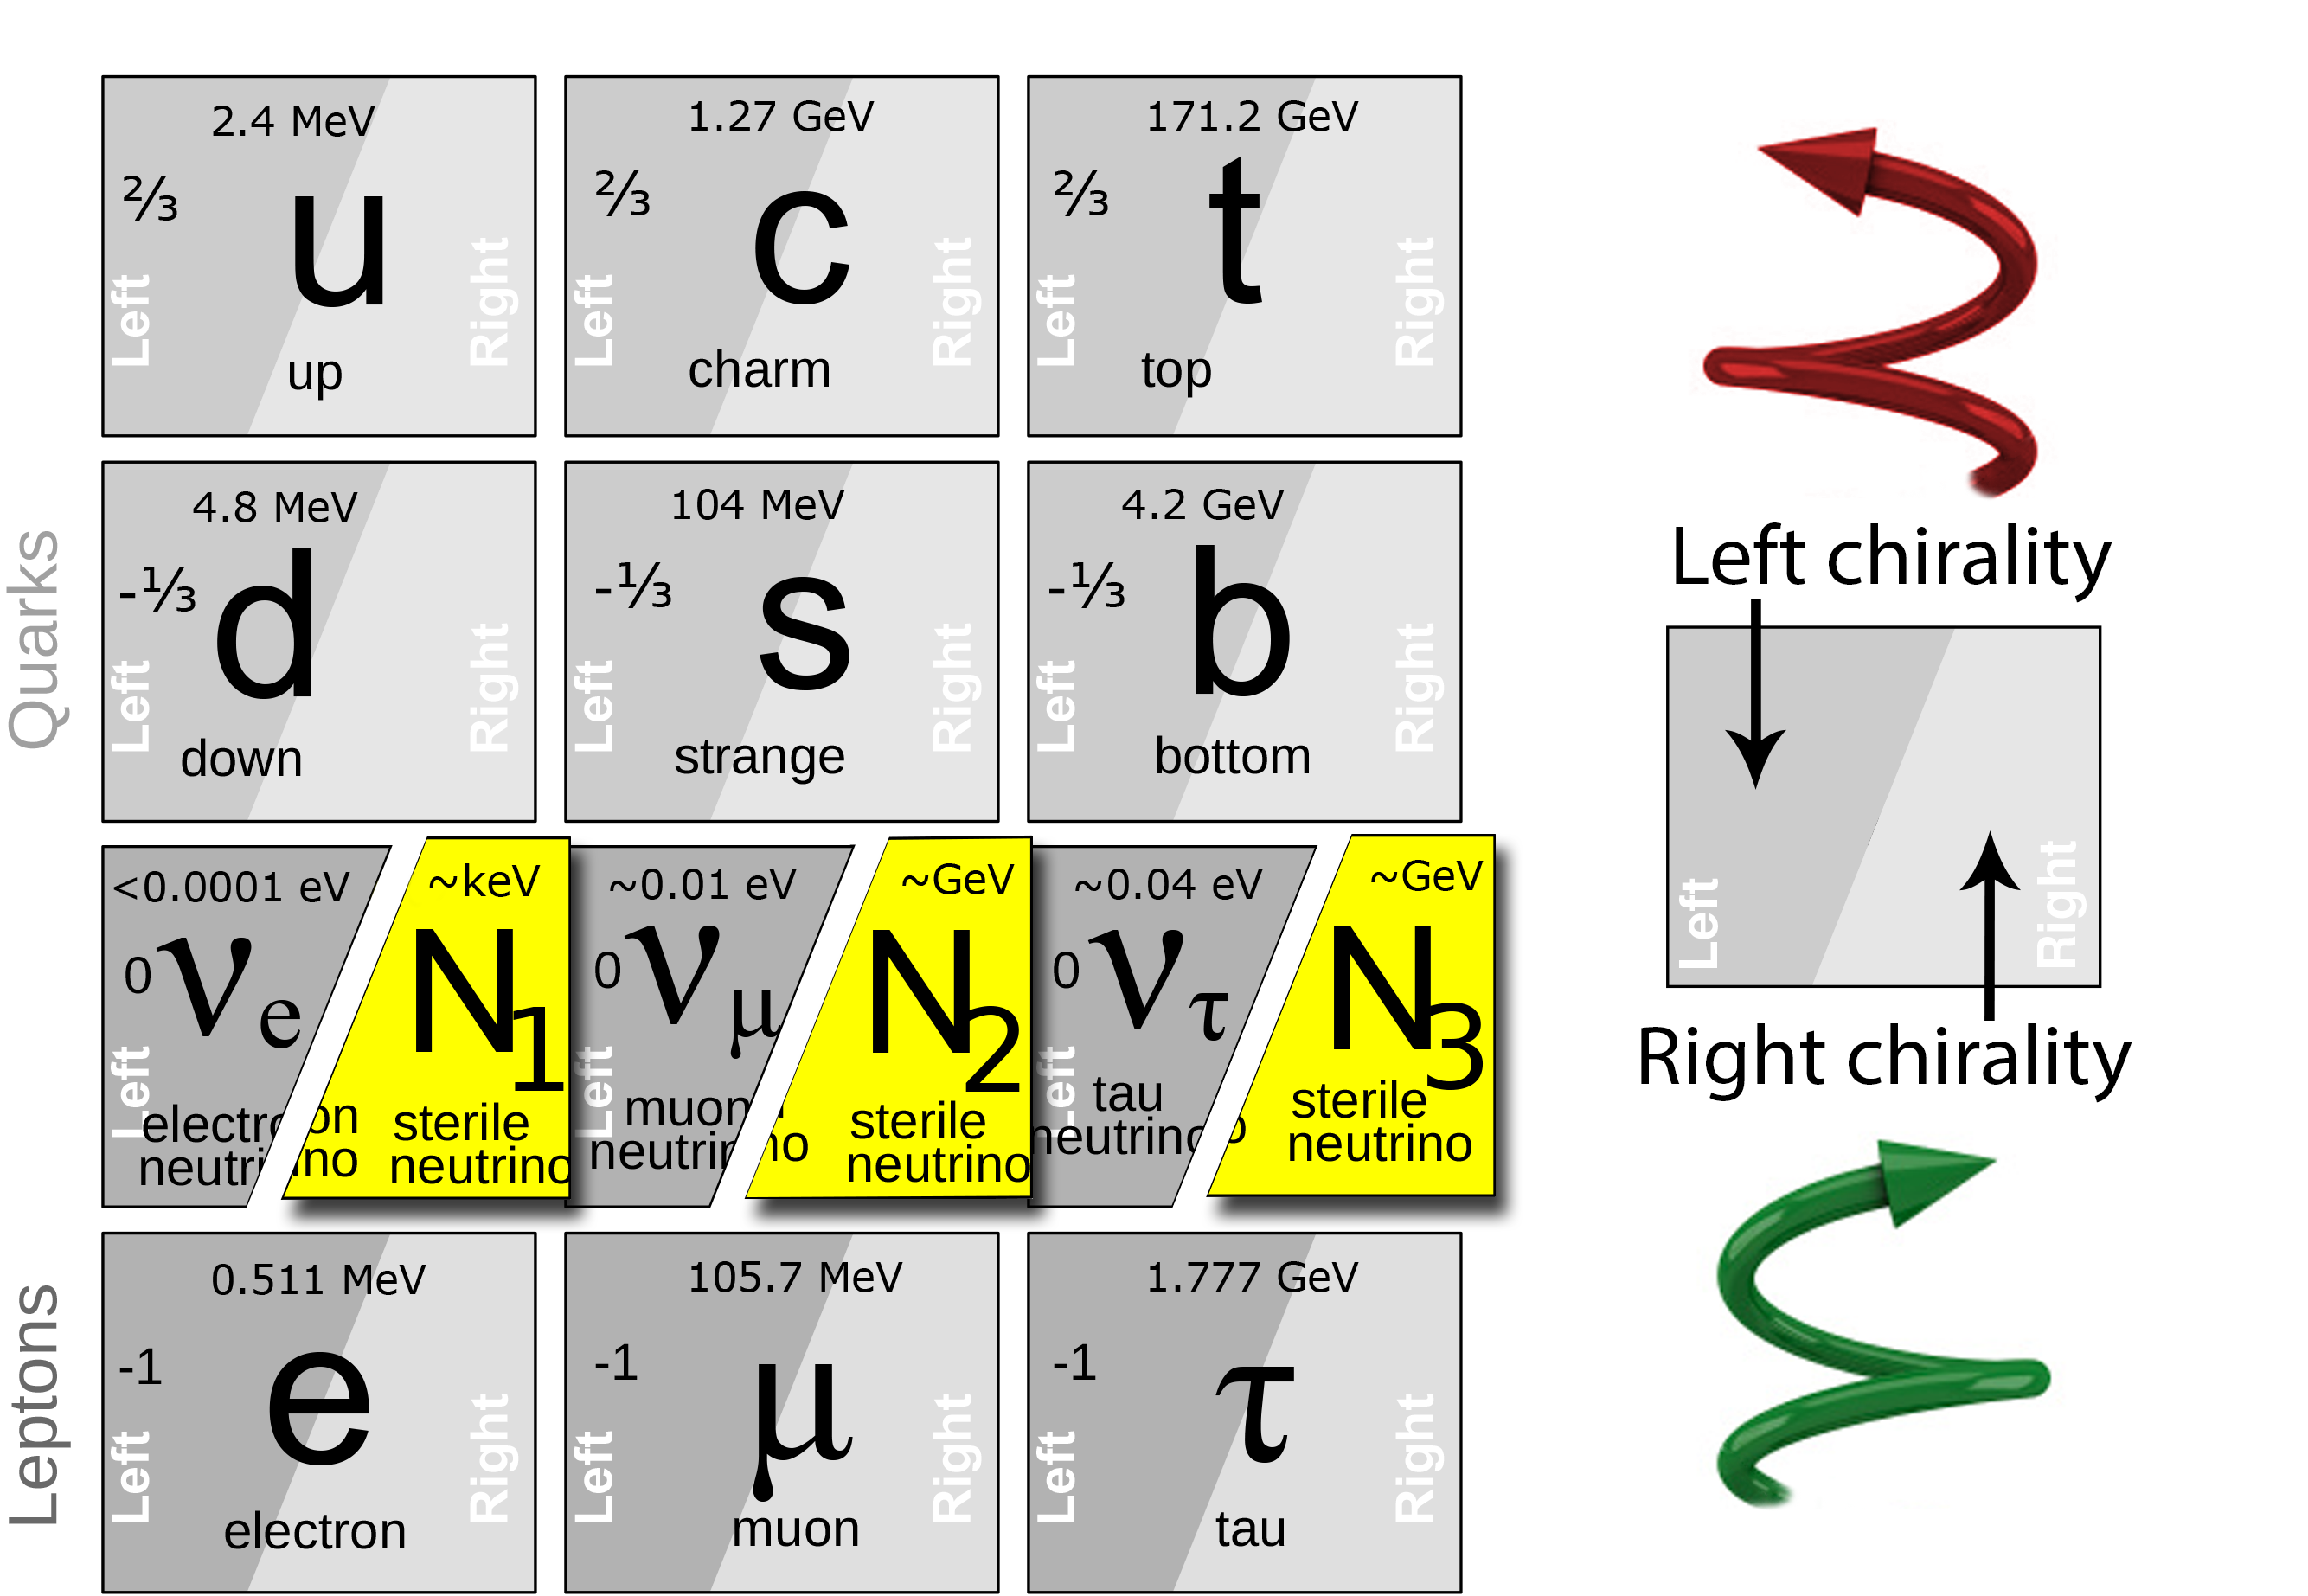
\includegraphics[width=0.8\columnwidth]{numsm.png}
\caption{Table comprising all fermions ($s/\hbar=1/2$) in the $\nu$MSM. The number in the top (\textit{resp.} left-side) of each panel is the particle's mass (\textit{resp.} electric charge). The only right chirality neutrinos in the SM are antineutrinos. In the $\nu$MSM, each of the lepton neutrinos has a heavy right-handed partner that has no lepton charge, in yellow. Credit: Alexey Boyarsky.}
\label{fig:numsm}
\end{center}
\end{figure}



\setcounter{chapter}{1}
\chapter{The Smooth Expanding Universe}
{\color{purple}\titlerule[2.5pt]}
\vspace{4pc}%
\label{chap:cosmology}
\tikz[remember picture,overlay] \node[opacity=0.3,inner sep=0pt] at (current page.center){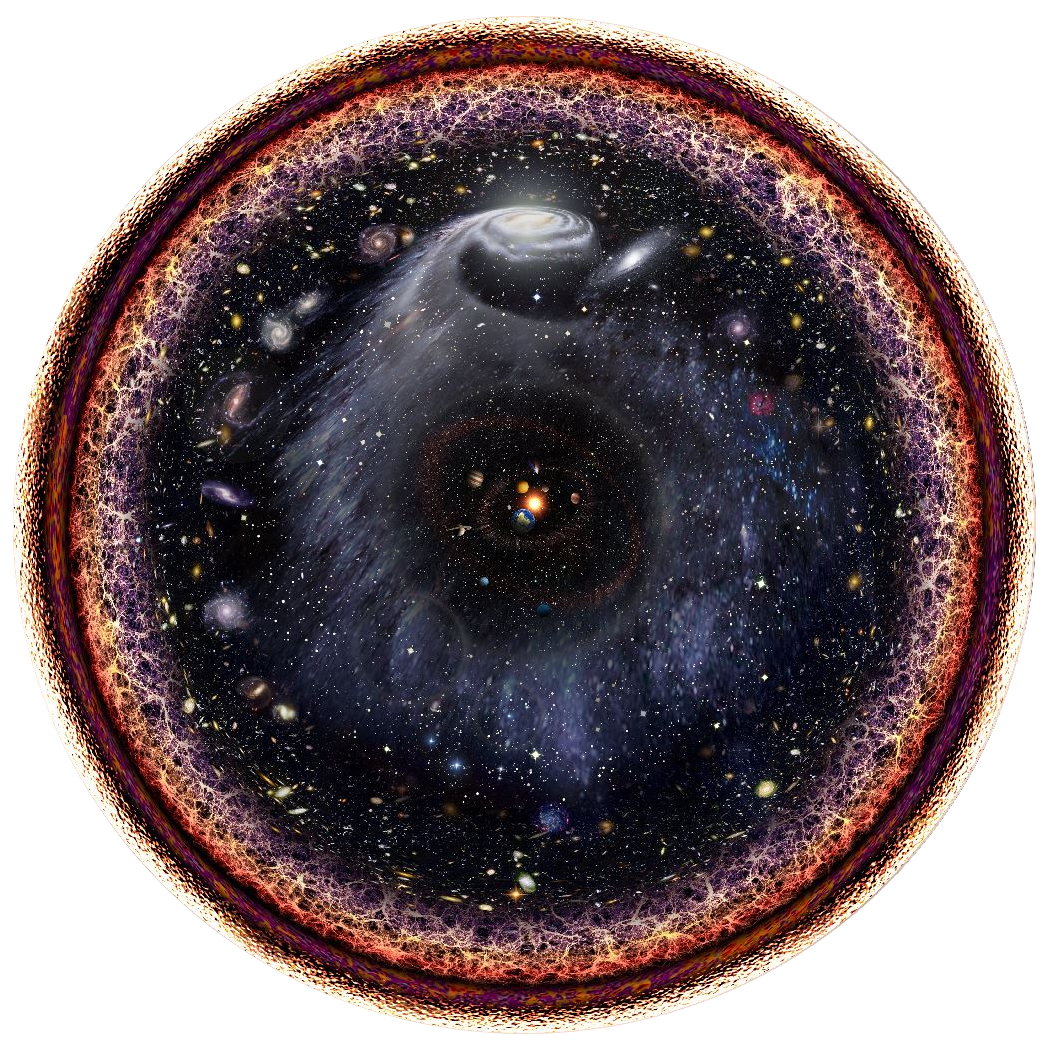
\includegraphics[width=20cm, height=20cm]{Cosmology/observable_universe.png}};
%{\centering
%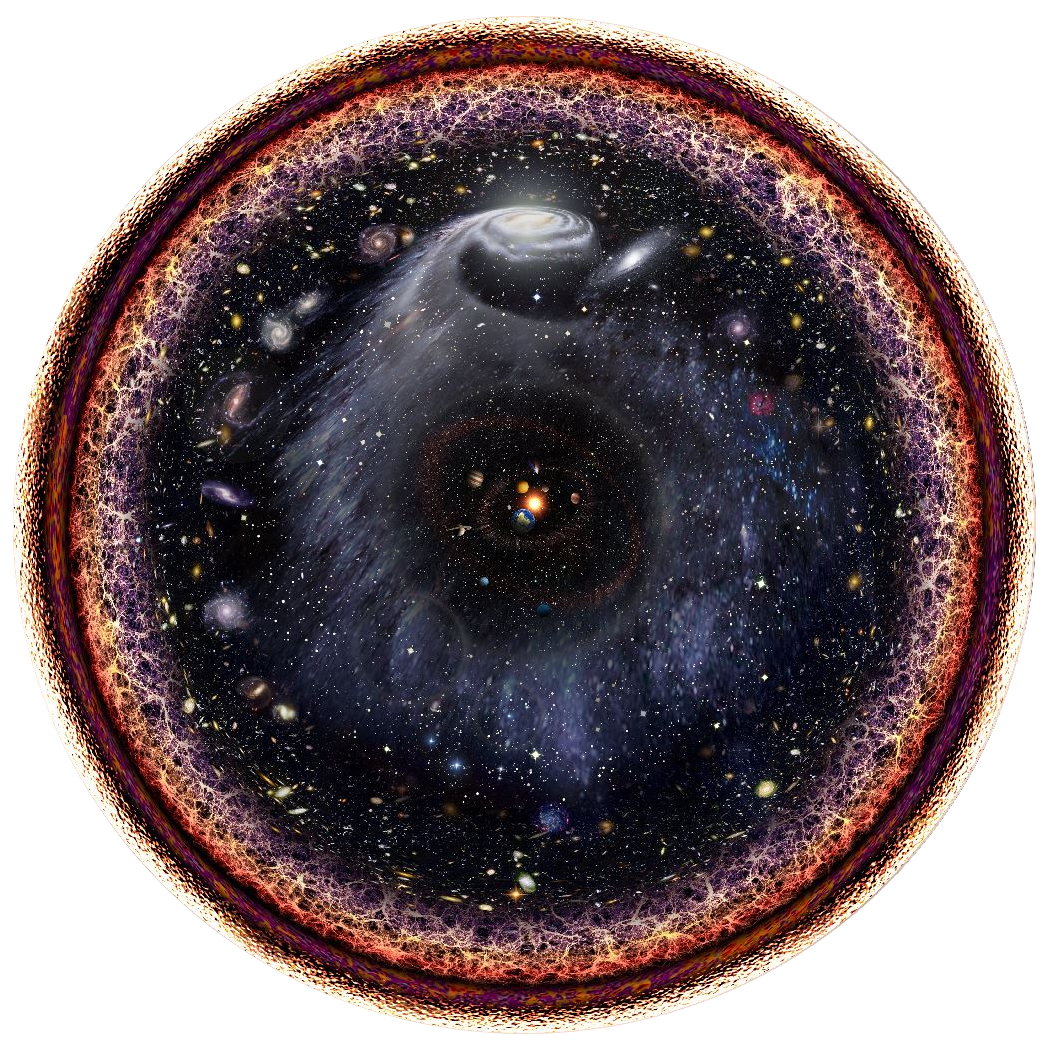
\includegraphics[width=\textwidth]{Cosmology/observable_universe.png}}
\clearpage

	\vspace*{3pc}
\begin{center}
\begin{minipage}{0.7\linewidth}
\hrule
\vspace{8pt}
{\huge\guillemotleft} ~The light shines in the darkness, and the darkness has not overcome it. {\huge\guillemotright}  \\
\vspace{2pt}
\begin{flushright}
--- \textsc{John 1:5}
\end{flushright}
\vspace{8pt}
\hrule
\end{minipage}
\end{center}
\vspace{3pc}

%\section*{Introduction}
\begin{intro}
{\color{purple}I}n the previous chapter, I detailed the impact of neutrino mass on the matter power spectrum. This was under the assumption that one can linearly perturb the density fields around their background value. However, since $\delta$ increases monotonically due to the attractive nature of the gravitational interaction, the approximation of linear theory eventually breaks down below some scale $k_0$. Linear theory remains valid as a perturbative treatment for $k < k_0$ where \\
\end{intro} 
\begin{equation*}
\begin{array}{c}
k_0^3 ~\vert \delta(k_0) \vert^2 \sim 1 \\
\Leftrightarrow \\
\Delta^2 (k_0) \sim 1 \\
\Leftrightarrow \\
\sigma^2 (1/k_0) \sim 1
\end{array}
\end{equation*} \\ For higher $k$ values, the evolution of $\delta$ is said to be \emph{non-linear}. One must explicitely solve the gravitational interactions between particles with numerical simulations. This is layed out in the following chapter. In the present chapter, I lay out how the power spectrum can be measured in the non-linear regime. In Sec.~\ref{sec:p1d}, I introduce quasi-stellar objects, which are the brightest sources of light in the Universe. The spectrometric properties of their light observed with Earth telescopes give us valuable information on their environment through their atomic spectral emission lines. The absorption lines, on the other hand, yield information on the intergalactic medium in which their light travels. A particular region of interest is the region blueward of the Lyman-alpha emission line, which entails the redshift and density of Hydrogen absorbers along the quasar line-of-sight. Known as the Lyman-alpha forest, it is a very active area of research for both extragalactic astrophysicists and cosmologists. I also introduce the main observable for this work: the power spectrum of the transmitted flux fraction in the Lyman-$\alpha$ forest of quasars. In Sec.~\ref{sec:pfdata}, I describe three sets of quasar samples taken from large scale structure surveys, from which I compute the Lyman-alpha power spectrum. 


	\section{The Geometry of the Universe}
	\label{sec:geometry}
	\vspace*{1pc}

Cosmology, the \textit{Logos} or inquiry into the world, is by no means a recent endeavor. What I describe in this section is our current interpretation of the \textit{Cosmos} we inhabit. The basic axioms that we rely on are that \\
\begin{itemize}
\item[$\bullet$] the cosmological principle, \textit{i.e.} the Universe is spatially homogenous and there are no special reference frames or observers\footnote{known as the Copernican Principle}, and
\item[$\bullet$] general relativity is the correct description of gravity, and \\
\end{itemize} The former is observationally motivated, and it has been proven that the distribution of matter is \emph{statistically} homogenous and isotropic to within $10^{-5}$ on large enough scales, \textit{i.e.} beyond a few Gpc\footnote{$1~\mathrm{Gpc} = 10^3~\mathrm{Mpc}$, where a Mpc is the typical physical distance between two galaxies.}. Several missing pieces make our interpretation incomplete, however, since general relativity isn't predictive at the singularity of black holes, and because of observational oddities such as dark energy, the horizon problem \textit{etc}. Our current incomplete picture rests on the observation that the Universe is in a perpetual expansion state. In this section, I describe the general relativity framework in which this observation is interpreted.

\subsection{The Geometry of Spacetime}

It is arguably during the 1930's that \emph{modern} cosmology was born. Following Vesto Slipher's and Edwin Hubble's discovery of extra-galactic nebul{\ae} --- which many turned out to be entire galaxies in their own right --- it was apparent that the Universe was not a static system. The consistent redshifting of these objects' light with their distance from us, regardless of where they are in the sky, was evidence that the Universe was expanding in a homogenous and isotropic manner, owing to the observation that there seemed to be no center from which the expansion was occuring and that the expansion was similar in any direction one looked. Making sense of this startling observation in the framework of the freshly developped general relativity required introducing a particular system of coordinates that is unchanging with this expansion.
One can write the physical coordinate of an object as $x(t) = a(t) \chi$ with $a$ the scale factor and $\chi$ the (time independant) coordinate of that object in that \emph{comoving} system.
Because of homogeneity, the scale factor is homogenous in space: $a(\vec{x}, t) = a(t)$. The physical velocity can be expanded into two terms:
\begin{equation}
\label{eq:hubble_flow}
\begin{array}{cl}
\cfrac{d x}{d t} &= \cfrac{d a }{d t} \chi + a(t) \cfrac{d\chi}{dt}\\
&=\cfrac{1}{a}\cfrac{da}{dt} x + a \dot{\chi}\\
&= H x + v_{\mathrm{pec}}
\end{array}
\end{equation} \\ where the right-most term is the galaxy's peculiar velocity, \textit{i.e.} its velocity with respect to the comoving coordinate system. The left-hand term is known as the Hubble flow. The (logarithmic) rate of change in the scale factor is known as the \textbf{expansion rate}, also known as the Hubble function:
\begin{empheq}[box=\mymath]{equation}
\label{def:Hubble}
H = \frac{1}{a} \frac{da}{dt}
\end{empheq}


\subsubsection{The Fabric of Spacetime}

The isotropic and homogeneous characteristics of the expansion implies, from a mathematical point of view, that only 2 parameters fully determine the geometry of the Universe: the scale factor $a$ which can only be a (undetermined) function of time because of homogeneity and a global curvature parameter $\kappa$ which must be constant because of isotropy. The geometry on any vector space including the 4-dimensional spacetime of relativistic physics is determined by the dot product $\pmb{g}$. It is the bilinear, non-degenerate symmetric form that verifies \\

\begin{eqnarray}
\pmb{g}: ~~ \begin{array}{ccc}
\mathbb{R}^n \times \mathbb{R}^n & \longrightarrow &\mathbb{R}\\
\left( \vec{u}, \vec{v} \right) & \longmapsto & \vec{u} \cdot \vec{v} = \displaystyle \sum_{i=1}^{n}\sum_{i=1}^{n}~g_{ij} u^i v^j
\end{array}
\end{eqnarray} \\

The form $\pmb{g}$ is bilinear in $\vec{u}$ and $\vec{v}$ and so defines a tensor, called the metric tensor on $\mathbb{R}^n$, or \textbf{metric} for short. Its components\footnote{see Appendix~\ref{apx:tensors}} $g_{\mu \nu}$ are the dot product of the basis vectors $\left( \hat{e}_1, \hat{e}_2, \hdots, \hat{e}_n \right)$ in which $\vec{u}$ and $\vec{v}$ are expressed:
\begin{equation}
g_{ij} \doteq \pmb{g} \left( \hat{e}_i, \hat{e}_j \right)
\end{equation} In Euclidian space, it is always possible to define a unitary orthogonal basis. In this basis, the components of the metric are therefore the Kronecker symbol because of the orthonormalisation identities: $\hat{e}_i \cdot \hat{e}_j = \delta_{ij}$. Because $\pmb{g}$ is non-degenerate, the inverse metric exists and its contravariant components verify $g^{i k} g_{k j} = \delta^i_j$ where I use the conventional implicit summation over repeated indices. In relativity, the time component is incorporated along with the spatial coordinates in a 4-vector: $\pmb{X} = (-ct, \vec{x})$, such that the path of any free-falling massless particle has a null 4-position: $\pmb{X}^2 = 0$, which is another way of expressing $r = ct$ where $r^2 = x^2 + y^2 + z^2$. The dot product is always implicitly performed with respect to the metric. Given the minus sign in the definition of 4-vectors, the components of the metric tensor in relativity are the Minkowski symbol ($\neq$ Kronecker): \\

\begin{equation}
\label{eq:Minkowski}
g_{\mu \nu} \doteq \hat{e}_{\mu} \cdot \hat{e}_{\nu} = \eta_{\mu \nu} = \left\{ 
\begin{array}{rl}
-1 & \text{if}~\mu = \nu = 0\\
1 & \text{if}~\mu = \nu \neq 0\\
0 & \text{if}~\mu \neq \nu\\
\end{array}
\right. = \left(
\begin{array}{rccc}
-1 & 0 & 0 & 0\\
0 & 1 & 0 & 0\\
0 & 0 & 1 & 0\\
0 & 0 & 0 & 1
\end{array}
\right)
\end{equation} \\ The negative time component signature apparent in expression~\ref{eq:Minkowski} shows that spacetime is non-Euclidian contrary to $\mathbb{R}^3$ in classical physics. The dot-product is \emph{not} defined positive in relativity since vectors can have negative 4-distance $ds^2 = g_{\mu \nu}dx^\mu dx^\nu$. I am using the convention of labelling the indices with greek letters ($\mu, \nu, \alpha, \beta$). Notice the $\mu=0$ component for time is expressed in units of $c$ such that the orthogonal basis is unitary. In the framework of cosmology, it is generally more useful to adopt the opposite convention with respect to general relativity: with the time component being a positive quantity such that time-like worldlines, \textit{i.e.} curves in spacetime linking two causally connected events, are seperated by a positive distance. \\

\subsubsection{The Robertson Walker metric}

As stated, there is always a system of coordinates in which the components of the metric tensor can be expressed as Eq.~\ref{eq:Minkowski}, at the sacrifice of allowing the coordinate system to \emph{not} pertain to an inertial frame of reference. In a Universe that expands uniformly in all directions, one can find such a \emph{comoving} coordinate system, introduced at the start of this section. Objects moving apart in the Hubble flow (left term of expression \ref{eq:hubble_flow}) are at rest in this comoving coordinate system ($v_{\mathrm{pec}}=0$). The elemental distance $d\ell$ in the 3-dimensional hypersurfaces of spacetime (the purely spatial components of events, labelled by latin indices $i, j, k$) can be expressed in spherical coordinates centered on an observer:
\begin{equation}
\label{def:dell}
d\ell^2 = \frac{dr^2}{1-\kappa r^2} + r^2 d\Omega^2
\end{equation} \\ where $d\Omega^2 = d\theta^2 + \sin^2 \theta ~d\varphi^2$ is the elemental solid angle. The spherical coordinate system centered on an observer is a natural choice in an isotropic Universe, which we assume here in addition to the Copernican (or ergodic) principle, which states that there is no special observer. Both of these conditions, known as the \emph{cosmological principle}, assures spatial homogeneity. From here onwards, I use spatial homogeneity and isotropy  interchangeably with the cosmological principle, even thought the former is a statement about the global geometry of spacetime while the latter is its observational consequence. Since the vector propagating time intervals is perpandicular to all three spatial directions: $\hat{e}_0 \cdot \hat{e}_i = 0$, we can consider spatially homogenous and isotropic hypersurfaces perpandicular to time which have constant global curvature. Because of isotropy, it is possible to rescale the constant curvature parameter $\kappa$ such that \\
\begin{equation}
\kappa = \left\{
\begin{array}{rl}
+1 & \text{for positively-curved space, like 3-spheres}~ \mathbb{S}^3\\
0 & \text{for flat space, like Euclidian}~ \mathbb{R}^3\\
-1 & \text{for negatively-curved space, like 3-hyperboloidal saddles}~ \mathbb{H}^3
\end{array}
\right.
\end{equation} \\
In the first, second and third case respectively, triangles defined between three points have angles that sum to more, exactly and less than $\pi$ radians, and the circumference of a circle is more, exactly or less than $\pi$ in units of its diameter (see Fig.~\ref{fig:geocurv}). \\

\begin{figure}
\begin{center}
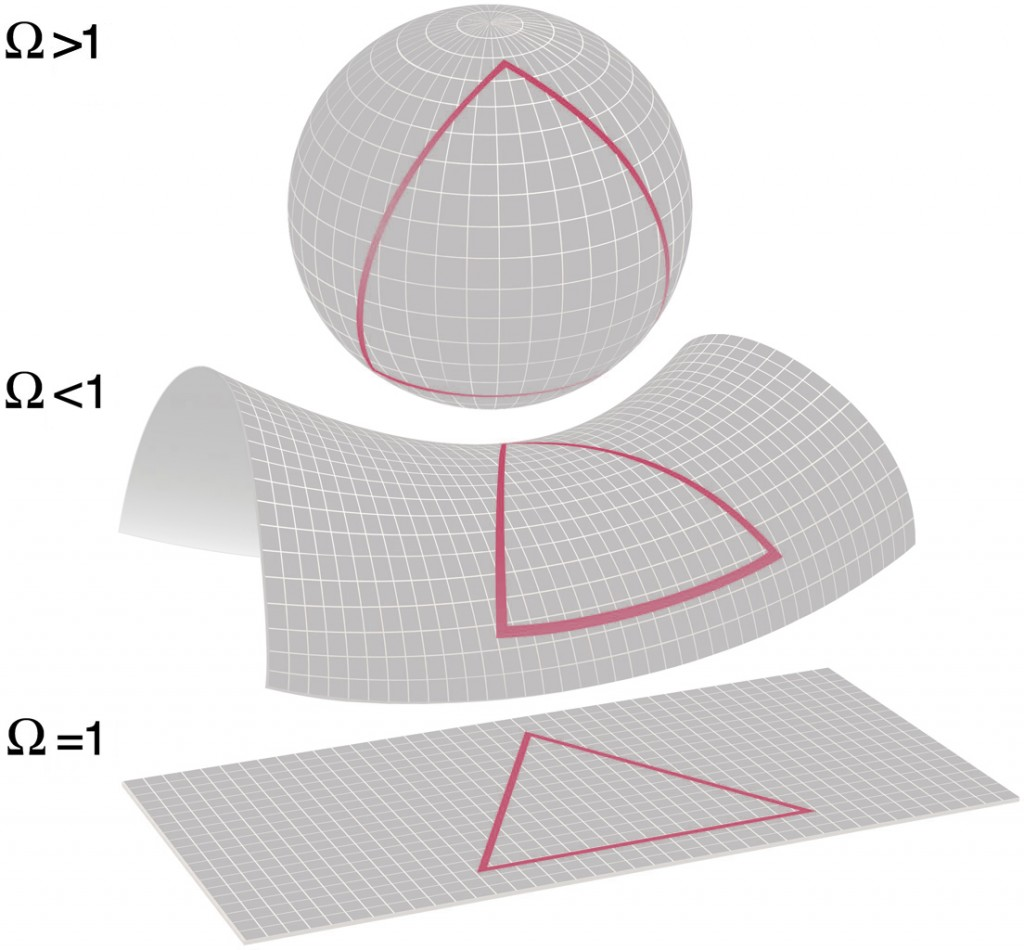
\includegraphics[width=0.75\columnwidth]{Cosmology/Big-Bang-shape.jpg}
\caption{The three categories of global geometry of a 2-dimensional Universe embedded in a 3-dimensional manifold. The critical density in its own units $\Omega$ is defined in expression~\ref{def:omega}. Credit: NASA/Hubble, public domain.}
\label{fig:geocurv}
\end{center}
\end{figure}


The simplest metric describing the geometry in a homogenous and isotropic expanding (or contracting !) Universe is the Robertson Walker metric, \textit{a.k.a.} the Friedmann Robertson Walker (FRW) metric. The line element is\\

\begin{equation}
\label{eq:RWmetric}
ds^2 = a^2 (\tau) \times \left( d\tau^2 - d\ell^2 \right)
\end{equation} \\ where the scale factor is factored out to define a \emph{conformal time} interval $d\tau = dt/a(t)$ which is the amount of time elapsed in between two events separated by a comoving elemental distance\\

\begin{equation}
d\chi = \frac{dr}{\sqrt{1 - \kappa r^2}}
\end{equation} \\ Depending on the global constant curvature of the Universe, the radial and comoving coordinates are linked by\\

\begin{equation}
\label{eq:RWmetric_space}
d\ell^2 = \gamma_{ij} dx^i dx^j = d\chi^2 + S^2_{\kappa} (\chi) d\Omega^2
\end{equation} \\ where $S_{+1, 0, -1} (\chi) = (\sin \chi, \chi, \sinh \chi)$ and $\pmb{\gamma}$ is the metric restricted to spatial coordinates only. 


\subsection{Motion Through Spacetime}

I've described the geometry of the Universe, which is useful in measuring distances between objects. The dynamics of objects in the Universe is all embeded in the FRW metric, and depends on whether the object of study is relativistic or not, which I lay out in this subsection.

\subsubsection{Equations of Motion}

Newton's principle of inertia states that an object's velocity is constant in an inertial frame of reference unless acted upon by a force, in which case the amplitude of the force equals the rate of change in the object's momentum. In the absence of any exterior interactions, the principle of inertia yields the conservation of kinetic energy $p^2 / 2m$ where $\vec{p}$ is the particle's linear momentum, which can be written as \\

\begin{equation}
\label{eq:kinetic}
\frac{\partial}{\partial t} \left( \frac{p^2}{2m} \right) = \vec{0} = \vec{p} ~ \frac{\partial}{\partial t} \vec{p}
\end{equation} \\

In general relativity, the motion of an object through curved (non-flat) space rids of the notion of a gravitational force. Gravity is essentially a property that emerges from different reference frames in a non-uniform metric. To get the equivalent of the point particle's mass and its equation of motion, we must define two quantities which are intrinsically defined on the particle's world line and do not depend on any observer (not everything is relative in relativity !). Given its 4-position $\pmb{X} = (x^0, \vec{x})$, the particle's 4-velocity and 4-momentum are respectively defined as:
\begin{align}
\pmb{U} &\doteq \frac{1}{c} \frac{d \pmb{X}}{dt}\\
\pmb{P} &\doteq m \frac{d \pmb{X}}{dt} = \left( \frac{E}{c}, \vec{p} \right)
\end{align} where $E$ is the total energy and $dt$ is the particle's \emph{proper time} defined as $c^2 dt^2 = ds^2$. These expressions introduce the particle's \emph{rest mass}, $m \geq 0$, as defined in the framework of general relativity, again an intrinsic property independant of any observer. Notice that the 4-velocity is defined as unitary, and so it follows that
\begin{align}
\label{eq:4velocity}
&\pmb{U} \cdot \pmb{U} = 1
&\pmb{P} \cdot \pmb{P} = m^2 c^2
\end{align} Photons obey $\pmb{P} \cdot \pmb{P} = 0$ and hence are massless\footnote{but they have energy}. Space-like momenta verify $\pmb{P} \cdot \pmb{P} < 0$ which translates into negative rest mass for hypothetical tachyons. In the absence of any non-gravitational interactions, the point particle's 4-momentum is expected to obey an expression similar to Eq.~\ref{eq:kinetic}. Such an equation, known as the \emph{geodesic} equation, requires differentiating along all directions with a proper derivative. In differential geometry, this is the covariant derivative $\pmb{\nabla}$ which is defined such that for a given 4-vector $\pmb{x} = (x^0, \vec{x})$,
\begin{equation}
\label{eq:connection_x}
\pmb{\nabla}_\mu x^{\nu} = \partial_\mu x^{\nu} + \Gamma^{\nu}_{\mu \alpha} x^{\alpha}
\end{equation} where $\Gamma$ is the Levi-Civita connection\footnote{see Appendix~\ref{apx:covariant}} on metric $\pmb{g}$ and I've used the notation $\partial_\mu \doteq \partial / \partial x^\mu$. The components of the particle's 4-velocity, or equivalently its 4-momentum, are linked through the metric connection via the geodesic equation, which is our sought-out equivalent of Eq.~\ref{eq:kinetic}: \\
\begin{empheq}[box=\mymath]{equation}
\label{eq:geodesic_p}
P^{\mu} \pmb{\nabla}_{\mu} P^{\nu} = 0
\end{empheq} \\

In terms of the 4-velocity, one can rewrite it to find the more conventional formula linking the spatial coordinates and their covariant derivatives with the Levi-Civita connection (using Eqs.~\ref{eq:connection_x},\ref{eq:4velocity}):
\begin{equation}
\label{eq:geodesic_u}
\begin{array}{cl}
0 &= U^{\beta} \pmb{\nabla}_{\beta} U^{\alpha}\\
&= U^\beta \partial_\beta U^\alpha + \Gamma^{\alpha}_{\mu \nu} U^\mu U^\nu\\
&= \ddot{X}^\alpha + \Gamma^{\alpha}_{\mu \nu} \dot{X}^\mu \dot{X}^\nu
\end{array}
\end{equation}

\subsubsection{The Expanding Universe}

The FRW metric features homothetic symmetries which make it invariant under rescaling of the following coordinates with the help of a scalar $\lambda \in \mathbb{R}$:
\begin{align*}
r &\mapsto \lambda^{-1} r\\
a &\mapsto \lambda a\\
\kappa &\mapsto \lambda^2 \kappa
\end{align*} As such, $a$ can be rescaled by its current value $a_0 = a(t_0)$ so that the scale factor is a dimensionless function of time in $0 \leq a(t) \leq 1$, and both $r$ and $1/\sqrt{\kappa}$ inherit a dimension of length. As such, the scale factor has physical meaning only in a positively-curved space, where it is the radius of the 3-sphere in units of its current radius. In flat space, only its rate of change $d \ln(a) / dt$ has physical meaning, which I've introduced in expression~\ref{def:Hubble} as the expansion rate. It appears in one of the non-zero connection given by the Levi-Civita symbols on the spatial part of the FRW metric (Eqs.~\ref{eq:RWmetric} and \ref{eq:RWmetric_space}):
\begin{equation}
\begin{array}{cl}
\Gamma^{i}_{0j} & = \cfrac{1}{2} \displaystyle\sum_{k=1}^{3} \gamma^{i k} \left( \cfrac{\partial \gamma_{i k}}{\partial x^0} + \cfrac{\partial \gamma_{0 k}}{\partial x^i} - \cfrac{\partial \gamma_{0 i}}{\partial x^k}\right) \\
& = \cfrac{\gamma^{ii}}{2} \cfrac{\partial \gamma_{ii}}{\partial x^0}\\
& = \cfrac{\dot{a}}{a} \delta^i_j
\end{array}
\end{equation} This new time function $H(t) \doteq \dot{a}/a$ is an observable quantity that is independant of the spatial coordinates. It expresses the rate at which any two given astrophysical objects move from one another\footnote{this, of course, assumes the objects are far enough apart to neglect their local spacetime metric, which is why it does not apply to systems bound within galaxies such as our solar system}. It is profound to note that the scale factor is intrinsically linked to the metric. The homogeneity of the FRW metric assures that the spatial components of the 4-momentum are divergencefree: $\partial_i P^\mu = 0$ so that the $\mu=0$ component of the geodesic equation~\ref{eq:geodesic_p} can be rewritten
\begin{equation}
\label{eq:energy}
E  \frac{dE}{dt} = - \Gamma^0_{ij} P^i P^j = - \frac{\dot{a}}{a} p^2
\end{equation} where $E/c = P^0$ and $\vec{p}^2 = a^2 \gamma_{ij} P^i P^j$ the particle's 3-momentum. Eq.~\ref{eq:energy} is the general relativity equivalent of the well-known relation from special relativity
\begin{equation}
E^2/c^2 = p^2 + (mc)^2 
\end{equation} with $m^2 = g_{\mu \nu} P^\mu P^\nu$. \\

\begin{figure}
\begin{center}
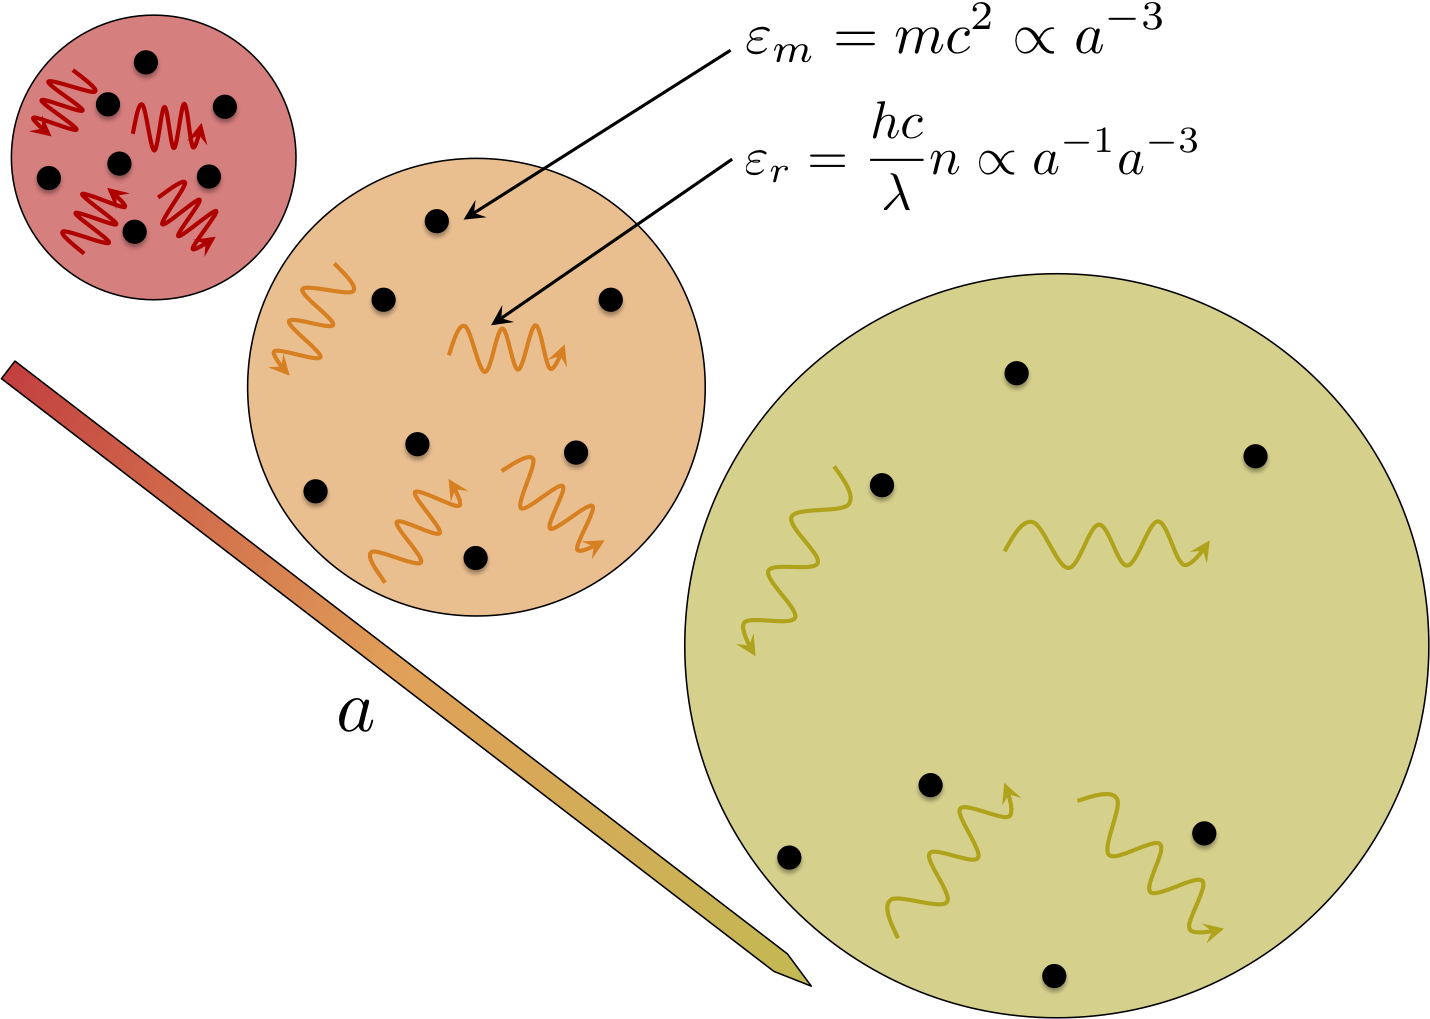
\includegraphics[width=0.75\columnwidth]{Cosmology/mr.png}
\caption{illustration of the evolution of radiation and non-relativistic matter energy density with scale factor. Radiation density decreases as the volume expands, just as for matter, but their associated wavelength gets stretched as well.}
\label{fig:expa}
\end{center}
\end{figure}


For non-relativistic particles, the rest energy dominates over the kinetic term. Notating $v^i = dx^i / dt$ the components of their comoving peculiar velocity, the magnitude of their 3-velocity is $v^2 = a^2 \gamma_{ij} v^i v^j$ and so  \\

\begin{equation}
P^i = m \frac{dt}{ds} v^i = \frac{mv^i}{\sqrt{1-a^2 \gamma_{ij} v^i v^j}} = \frac{m v^i}{\sqrt{1-v^2}}
\end{equation} \\
For relativistic particles on the other hand, the kinetic energy term is preponderant over mass, and so $EdE = pdp$ which yields\\

\begin{equation}
\label{eq:momentum_ur}
\begin{array}{ccc}
\cfrac{\dot{p}}{p} = \cfrac{\dot{a}}{a} = 0 & \Leftrightarrow & p \propto a^{-1}
\end{array}
\end{equation} \\ for relativistic particles. The photon's 4-momentum\footnote{the $\gamma$ index stands for ``photon'', not for a spactime component} $\pmb{P}_\gamma = \left( h \nu / c, -1, -1, -1 \right)$ is proportional to its frequency $\nu = c/\lambda$. It follows from Eq.~\ref{eq:momentum_ur} that a photon's wavelength scales as $a(t)$. Since everything we deduce from the Universe comes from the light emitted by distant luminous objects, this shift in the photon's wavelength red-wards as the Universe expands has to be taken into account as it conceals the expansion rate along its free-falling flight. It is useful to define the quantity $z$ such that \\

\begin{empheq}[box=\mymath]{equation}
\label{def:redshift}
1 + z \doteq \frac{\lambda}{\lambda_0} = \frac{a_0}{a(t)} \geqslant 1
\end{empheq} \\
where $\lambda_0$ is the photon's wavelength in its proper inertial frame at time of emission $t$ and $\lambda$ its wavelength as measured by an observer at time $t_0$ in their frame of reference. Because $a(t) \leqslant a_0 = 1$, $z$ is always positive, meaning the photon's wavelength is always shifted redwards. As such, $z$ is known as the cosmological \textbf{redshift}. It is a purely observational quantity \emph{that does not require a cosmological model}. A photon's wavelength will be redshifted due to 3 main effects:\\
\begin{itemize}
\item[$\bullet$] the Einstein effect, \textit{i.e.} the difference in magnitude of the gravitational field between the observer and the photon's source if the gravitational field is strong;\\
\item[$\bullet$] the Doppler effect, \textit{i.e.} the relative peculiar velocity between the source and the observer; and\\
\item[$\bullet$] the cosmological redshift, which is a pure consequence of the source and the observer being at different coordinates in a \emph{non-inertial} reference frame.\\
\end{itemize}
In this thesis, I study the light coming from very distant luminous objects, quasars, which I introduce in Sec.~\ref{sec:qso}. The light is emitted from a disk region around a supermassive black hole, far from where the Einstein effect can be noticeable. I am working under the assumption that galaxies and quasars are stationary in the comoving coordinate system. The total redshift is thus dominated by the cosmological redshift $z$, and as such I make no distinction between total and cosmological redshift. For objects in the Hubble flow, the cosmological redshift is linear with distance at first order. By expanding the scale factor into an infinite series,\\

\begin{equation}
\label{def:deva}
a(t) = \sum_{k=0}^{\infty} \left( t-t_0 \right)^k \frac{d^k a}{dt^k} (t_0)= a_0 \times \left[ 1 + (t-t_0) \left. \frac{\dot{a}}{a} \right\vert_{t_0} + (t-t_0)^2 \left. \frac{\ddot{a}}{a} \right\vert_{t_0} + \hdots \right]
\end{equation} \\ we can identify the expansion rate as the first order term. The second order term is known as the acceleration parameter, more often rescaled as $\ddot{a} a / \dot{a}^2$. For objects close enough so that $t-t_0$ is negligeable with respect to the conformal age of the Universe,
\begin{equation}
\label{eq:hubble_approx}
z \simeq H_0 \times d
\end{equation} where $d = (t-t_0)$ in units of $c$. The current value of this function $H_0 = H(t_0)$ is often expressed in units of $100~\mathrm{km}~s^{-1}\mathrm{Mpc}^{-1}$ since the significant digits are not quite precice to this day, depending on which data set is used. Commonly, $h \sim 0.7$ within an uncertainty of $\sim 10~\%$, where
\begin{equation}
\label{eq:h}
H(t) = 100~h~\mathrm{km}\cdot s^{-1} \cdot \mathrm{Mpc}^{-1}
\end{equation} Since the scale factor is an undetermined function of time, so is its rate of change. When quoting values for $h$, unless specified otherwise, it is implicitely assumed to be at current time $t_0$. The $0$ subscript is removed for concision purposes as distances and most cosmological parameters are expressed in terms of $h$. The evolution of $a$ and $h$ in time depend mostly on the entropy density of the Universe and thus solving the thermodynamics of the Universe is required at very early times.




\subsection{The Warping of Spacetime}

As previously stated, what is experienced as a gravitational acceleration by an observer is, in general relativity, an inertial acceleration that manisfests due to spacetime curvature. The Newtonian limit is embedded in the so-called Einstein field equations, which quantify the local curvature of spacetime. In this subsection, I detail what is spacetime curvature and what its value is in the FRW metric that describes the Universe's global geometry.  
 
\subsubsection{Spacetime Curvature}

Imagine two travellers starting at the Earth's equator at different longitudes and both heading straight North. Even though they are on parallel trajectories, their paths \emph{will} cross at the North pole. The angles of the triangle their paths form with the segment seperating their starting positions on the equator sum to more than $\pi$ radians. This is due to the non-Euclidian nature of the surface of a spherical Earth. If you've ever wondered why something was missing as you flattened the skin of a ripe clementine after you've peeled it away from the fruit, you were not mistaking: there literally is something missing, preventing you from flattening it into a uniform and uninterupted $\mathbb{R}^2$ plane. The curvature of the spherical surface --- be it the skin of a clementine or the Earth's crust --- is intrinsically linked to the connection of its metric $\pmb{\Gamma}$. The reason our two travellers met on parallel lines is because the covariant derivatives are only comutative in flat space. In general relativity, the 4-dimensional spacetime at a point (event) $P$ is the tangential space at point $P$ of a 5-dimensional \textbf{manifold} $\mathbb{M}$ and is usually written as $\mathcal{T}_P(\mathbb{M})$. In general, given three vectors, $(\vec{u}, \vec{v}, \vec{w}) \in \mathcal{T}^3_P (\mathbb{M})$,
\begin{equation}
\label{def:riemann_curvature_def}
\vec{\nabla}_{\vec{u}} \vec{\nabla}_{\vec{v}}~ \vec{w} = \vec{\nabla}_{\vec{v}} \vec{\nabla}_{\vec{u}} ~\vec{w} + R(\vec{u}, \vec{v})~\vec{w}
\end{equation} where the endomorphism
\begin{eqnarray}
\begin{array}{ccc}
\mathcal{T}_P(\mathbb{M}) & \longrightarrow & \mathcal{T}_P(\mathbb{M})\\
\vec{w} & \longmapsto & R(\vec{u}, \vec{v})~\vec{w}
\end{array}
\end{eqnarray} is linear in $\vec{u}$ and $\vec{v}$ and so defines a tensor, known as the Riemann curvature. It quantifies the non-commutativity of the covariant derivative. Given the following property of the Levi-Civita connection (implicit in $\nabla$): 
\begin{equation}
\label{eq:doublecov}
\nabla^2_{\vec{u}, \vec{v}} = \vec{\nabla}_{\vec{u}} \vec{\nabla}_{\vec{v}}~ \vec{w} - \vec{\nabla}_{\vec{\nabla}_{\vec{u}}\vec{v}} \vec{w}
\end{equation} the Riemann curvature tensor can be identified as
\begin{equation}
\label{def:riemann_curvature}
R(\vec{u}, \vec{v}) = \nabla^2_{\vec{u}, \vec{v}} - \nabla^2_{\vec{v}, \vec{u}}
\end{equation} To illustrate its purpose, Fig.~\ref{fig:parallel_tranport} shows the parallel transport of $\vec{w}$ along $\vec{u}$ and then $\vec{v}$, in comparison to along $\vec{v}$ and then $\vec{u}$. If one starts from the North Pole and keeps pointing South while traveling due South to the equator, then East to a quarter of the circumference of the Earth and then North again to one's starting position, his/her final pointing direction will be $\pi/2$ radians off of its original direction. In Euclidian geometry, the Riemann curvature tensor is zero and transporting $\vec{w}$ along any path will not alter its direction; the covariant derivatives are commutative, and the sum of the angles of a triangle is always $\pi$ radians.\\

\begin{figure}
\begin{center}

\includegraphics[width=0.8\columnwidth]{Cosmology/parallel_transport.png}
\caption{The orange arrows all point ``southwards'', but since the Earth's Riemann curvature isn't null, the parallel transport of the orange vector along meridians and parallels does not conserve direction.}
\label{fig:parallel_tranport}
\end{center}
\end{figure}


The components of the Riemann curvature tensor can be expressed in terms of the Levi-Civita connection defined in Appendix~\ref{apx:covariant}: \\
\begin{equation}
\label{eq:Riemann_Tensor_explicit}
\begin{array}{cl}
R^i_{jk\ell} &\doteq dx^i \left( R(\vec{\partial}_k, \vec{\partial}_\ell) ~\vec{\partial}_j \right)\\
&= \partial_k \Gamma^i_{\ell j} - \partial_\ell \Gamma^i_{k j} + \Gamma^i_{k m} \Gamma^m_{\ell j} - \Gamma^i_{\ell m} \Gamma^m_{k j}\\
&= g^{im} R_{mjk\ell}
\end{array}
\end{equation} \\ The curvature $\mathcal{R}$ of the vector space being considered is simply the trace of the Riemann curvature tensor. For the 2-dimensional surface of the Earth, the curvature \textit{a.k.a.} the Ricci scalar\footnote{because it appears in the Ricci identity} is twice the inverse of its radius squared. For the FRW metric,
\begin{equation}
\label{eq:Ricci_scalar}
\mathcal{R} = g^{\mu \nu} R^{\alpha}_{\mu  \alpha \nu} = - 6 \left( \frac{\ddot{a}}{a} + \left( \frac{\dot{a}}{a} \right)^2 + 2 \frac{\kappa}{a^2} \right)
\end{equation} The Riemann curvature tensor with its first and third indices contracted $R^{\alpha}_{\mu  \alpha \nu} = R_{\mu \nu}$ has the same divergence as the metric tensor $\pmb{g}$ from which it is defined. The Einstein tensor, defined as $\pmb{G} = \pmb{R} - \mathcal{R}/2 ~\pmb{g}$, is thus divergence free. In fact, it is the only rank 2 tensor made from the second derivatives of the metric that features this property, which is useful in establishing the conservation of energy in the framework of general relativity. In order to do so, the warping of spacetime, encapsulated in the Einstein tensor, must be linked to its source and drain terms. In a Universe whose geometry is described by the FRW metric, the non-trivial components of  $G^\mu_\nu = g^{\mu \alpha} G_{\alpha \nu}$ are, using Eq.~\ref{eq:Riemann_Tensor_explicit} and Eq.~\ref{eq:Ricci_scalar} on Eq.~\ref{eq:RWmetric},

\begin{equation}
\label{eq:einsfrw}
\left\{
\begin{array}{l}
G^0_0 = 3 \left[ \left( \cfrac{\dot{a}}{a} \right)^2 + \cfrac{\kappa}{a^2} \right]\\
G^i_j = 2 \left[ \cfrac{\ddot{a}}{a} \left( \cfrac{\dot{a}}{a} \right)^2 + \cfrac{\kappa}{a^2} \right] ~\delta^i_j
\end{array}
\right.
\end{equation}


\subsubsection{Source Terms}

The source terms for the warping of spacetime must come from the local energy content. The rank 2 tensor encapsulating the energy of matter is the stress-energy tensor $\pmb{T}$ whose general covariant expressions of its components are moments of the distribution function \\
\begin{empheq}[box=\mymath]{equation}
\label{eq:nrj_general}
T_{\mu \nu} = \frac{g}{(2 \pi)^3} \int dP_1 dP_2 dP_3 ~\frac{P_\mu P_\nu}{\sqrt{-g} P^0} ~ f(x^i, P_j, \tau)
\end{empheq} \\ where $(-g)^{-1/2} = a^{-4}$ is the metric's trace. The distribution function $f$ is the probability of occupying a given state $(\vec{x}, \vec{P}, t)$ in phase space. The number of particles with $g$ spin states in phase-space volume\footnote{the density of states in a given phase-space is $g/ h^3$ or $g/(2 \pi)^3$ in units of $\hbar = h/2\pi$} $d^3\vec{x} d^3\vec{P} = dx^1 dx^2 dx^3 dP_1 dP_2 dP_3$ is given by \\
\begin{equation}
dN = \frac{g}{(2\pi)^3} ~f(x^i, P_j, \tau)~ d^3\vec{x} d^3\vec{P}
\end{equation} The numerical density of particles is therefore the zeroth moment of the distribution function:
\begin{equation}
\label{eq:number_density}
n(x^i, \tau) = \frac{g}{a^4} \displaystyle \int \frac{d^3P}{(2 \pi)^3} ~f(x^i, P_j, \tau)
\end{equation}

At any given time, the distribution function obeys the Boltzmann equation\\

\begin{empheq}[box=\mymath]{equation}
\mathbb{L}\left[ f \right] = \mathcal{C} \left[ f \right]
\end{empheq} \\ where the Liouville operator $\mathbb{L} \doteq d/ds$ is the derivative along the particle's worldline and the collision functionals $\mathcal{C}$ encapsulate all collision terms and are determined by particle physics.\\

The particle's individual 4-momentum in the FRW metric is
\begin{equation}
\pmb{P} = \left( \epsilon, \vec{q} \right)
\end{equation} with $\vec{q} = q \hat{q} = a \vec{p} = \vec{p}/T$ where $\vec{p}$ is the particle's \emph{proper} momentum as measured by an observer stationary in the comoving coordinate system and $\epsilon(q) = a E = E/T = \sqrt{a^2 m^2 + q^2}$. It is useful to use $\vec{q}$ and $\epsilon$ instead of $\vec{p}$ and $E$ since these quantities are not redshifted, hence we can call them the particle's comoving momentum and comoving energy. We can express the stress energy tensor's components in terms of these quantities, respectively the energy density, the flux of relativistic mass accross the surface normal to $x^i$ and the shear stress tensor:\\

\begin{equation}
\label{sys:stress_energy_tensor_components}
\left\{
\begin{array}{ll}
\rho c^2 = & T^0_0 = -\cfrac{1}{a^4} \displaystyle \int \cfrac{d^3q}{(2\pi)^3}~ \epsilon~ f(\vec{x}, \vec{q}, \tau)\\
\\
\vec{\varphi} c^2 = & T^0_i = \cfrac{1}{a^4} \displaystyle \int \cfrac{d^3q}{(2\pi)^3}~ q_i~ f(\vec{x}, \vec{q}, \tau) = - T_0^i\\
\\
\Sigma^i_j = & T^i_j = \cfrac{1}{a^4} \displaystyle \int \cfrac{d^3q}{(2\pi)^3}~ \cfrac{q^i q_j}{\epsilon}~ f(\vec{x}, \vec{q}, \tau)
\end{array}
\right.
\end{equation} \\

The diagonal elements of the shear stress tensor are known as normal stress \textit{a.k.a.} pressure $\mathcal{P}^i$ exerted on surface normal to $x^i$, while the non-diagonal elements
\begin{equation}
\Sigma^{i,j \neq i} = \sigma^{ij} = \frac{1}{2} \left( \frac{\partial v^j}{\partial x^i} + \frac{\partial v^i}{\partial x^j} \right)
\end{equation} correspond to shear 3-velocity ($\vec{v} = d\vec{x}/dt$) displacement on the surface normal to $x^j$ in the $x^i$ direction, known as anisotropic stress. Because the 4-momentum and 4-velocity are linked via $\pmb{P} = mc~\pmb{u}$, and since pressure is isotropic ($\mathcal{P}^i = \mathcal{P}$), one can write the stress energy tensor in the following tensoral form 
\begin{equation}
\pmb{T} = (\rho + \mathcal{P})~ \pmb{u} \otimes \pmb{u} + \mathcal{P}\pmb{g} + \pmb{\Sigma}
\end{equation} where $\otimes$ denotes the tensoral product.\\

In the spatially homogenous and isotropic background, spatial vectors are vanishing, \textit{i.e.} $\vec{\varphi} c^2 = \vec{0}$ and there is no anisotropic stress, \textit{i.e.} $\pmb{\sigma} = \pmb{0}$, hence the stress energy tensor is diagonal and its contravariant components are

\begin{equation}
\label{eq:stress_fluid}
T^{\mu \nu} = \rho \left[ (w+1) u^\mu u^\nu - w g^{\mu \nu} \right]
\end{equation} which one may recognize as the stress-energy tensor of a perfect fluid of 4-velocity $\pmb{u}$ with an equation of state linking its dynamic pressure $\mathcal{P}$ to the energy density:
\begin{equation}
\label{eq:eos}
\mathcal{P} = w \rho c^2
\end{equation} The perfect fluid approximation is technically \emph{not} valid in the sense that the components of the Universe are not fluids: dark matter for instance does not interact and so cannot define a pressure on its surroundings. However, in absence of anisotropic stress --- which holds true only in the unperturbed background --- the stress energy tensor has the mathematical form of a perfect fluid \emph{a posteriori}. In an abuse of language, we can thus treat the components of the Universe as a perfect fluid at first approximation. The fluid approximation still holds for first order perturbations, which I describe in the next chapter. However, the perturbed cosmological fluid is not perfect as it features anisotropic stress. \\

\subsubsection{From Einstein to Friedmann}

I now postulate (and do not demonstrate !) the Einstein field equations (EFEs), which link the Einstein tensor to the source terms of curvature. They are a set of 10 highly-coupled non-linear second-order differential equations whose solutions are the components of the metric tensor:
\begin{empheq}[box=\mymath]{equation}
\label{eq:EFEs_tensor}
\pmb{G} = \frac{8 \pi G}{c^4} \pmb{T}
%\end{equation}
\end{empheq} with $G$ the universal gravitational (or Newton) constant and the source term $\pmb{T}$ is the stress-energy tensor. \\

These field equations can be used to solve for the internal structure of white dwarfs or neutron stars (where the warping of spacetime is significant and a Newtonian description for the hydrodynamic equilibrium is inadequate), known as the Tolman-Oppenheimer-Volkoff (TOV) equations. In the framework of cosmology, we make use of the Einstein field equations in the opposite way: we postulate from the cosmological principle that the metric is the FRW metric and plug it into the EFEs to extract the conservation laws in the context of an expanding Universe. For the background, the Einstein tensor is diagonal, and so too must be the stress-energy tensor. This gets the number of independant field equations down to 4. Because of homogeneity and isotropy, the 3 spatial ones are redundant and the only 2 independant non-trivial equations are known as the Friedmann equations, using Eq.~\ref{eq:einsfrw}\\

\begin{equation}
\left\{
\begin{array}{lcl}
G^0_0 = 8 \pi G ~T^0_0 & \Rightarrow & \left( \cfrac{\dot{a}}{a} \right)^2 + \cfrac{\kappa}{a^2} - \cfrac{8 \pi G}{3} \rho = 0\\
G^i_j = 8 \pi G ~T^i_j & \Rightarrow & \cfrac{\ddot{a}}{a} + \cfrac{4 \pi G}{3} \left( 1+3w \right) \rho
\end{array}
\right.
\end{equation} \\ These equations are the equivalent of the Poisson and Euler equations of a fluid at rest in a comoving frame of reference. One can also get the continuity equation by either combining both Friedmann equations or using Eq.~\ref{eq:connection_x} on $0 = \pmb{\nabla \cdot G} = \pmb{\nabla \cdot T} = \pmb{\nabla}_\mu T^\mu_0$:
\begin{equation}
\label{eq:continuity}
\dot{\rho} + 3(1+w) H \rho = 0
\end{equation} Integrating Eq.~\ref{eq:continuity} to solve for the energy density $\rho$, 
\begin{equation}
\label{eq:rho}
\rho (t) = \rho (t_0) ~ a^{- 3(1+w)H(t)}
\end{equation} The first Friedmann equation along with the equation of state set the time evolution of the scale factor (heretofor undetermined):
\begin{equation}
a(t) = a_0 \times t^{\frac{2}{3 (1+w)}}
\end{equation} The cosmological perfect fluid considered here is \emph{not} mono-phase. It consists of all known (and unknown) particles. I conventionally adopt a very coarse-grain approach and consider the cosmological fluid as an admixture of two main components:\\
\begin{itemize}
\item[$\bullet$] relativistic matter, \textit{a.k.a.} \textbf{radiation}, which consists of all massless bosons including photons as well as fermions whose $\epsilon \simeq q$; and \\
\item[$\bullet$] non-relativistic matter, or \textbf{matter} for short, which consists of all partices whose $\epsilon \simeq a m$. \\
\end{itemize} To obtain the equations of state of these two main components, thereby explicitely determining the time evolution of the scale factor, we must determine the background temperature $T_\gamma$ from the thermodynamics of the Universe.

\clearpage
	
	\section{The Thermal History of the Hot Big Bang Model}
	\label{sec:thermal}
	\vspace*{1pc}

The momentum of a photon is the frequency of its wave packet in units of $\hbar$. The FRW metric encoding the geometry of the expanding Universe is a troublesome system of coordinates because it is not linked to an inertial frame of reference. As such, the conservation of energy expressed by the Friedmann equations only hold for a fluid \emph{at rest} in the comoving coordinate system. Free-falling photons (\textit{i.e.} when not being absorbed), are constantly mobile in this coordinate system. On distances negligeble with respect to its proper time (its comoving particle horizon), photons occupy more or less the same comoving coordinate and nothing drastic or unexpected happens. On distances comparable to its proper time however, the photon's momentum is drained by the very geometry of the spacetime in which it is moving, given by expression~\ref{eq:momentum_ur}. Just as non-inertial reference frames see the spawning of fake centrifugal forces, the non-inertial nature of the comoving coordinate system has the consequence of \emph{not} conserving energy. Energy \emph{is} conserved in a fake so-called comoving volume, which can be thought of as the volume that expands (or contracts) homogenously with $a^3$. This is precisely what the cosmological redshift entails: a property of comoving observers and not of space. Neglecting the source's gravitational potential and its peculiar velocity with respect to the Hubble flow, the wavelength of the photon as measured by an observer is redshifted by the amount given in the defining relation~\ref{def:redshift}. Since the wavelength of the photon is the inverse of its Boltzmann temperature in units of $\hbar c/k_b$, it follows that the background teperature scales inversely with the scale factor.
\begin{equation}
\begin{array}{c}
\lambda(t) = \cfrac{\hbar c}{k_b T(t)} \propto a(t)\\
\Leftrightarrow\\
T(t) = T_0 \times \cfrac{a_0}{a(t)} = T_0 \times (1+z)
\end{array}
\end{equation}
Just as we've been introduced to the Friedmann equations as the Navier Stokes equations of a fluid at rest in the comoving coordinate system, let us venture into the thermodynamics of the Universe's contents in a comoving volume (sometimes called a covolume) where the temperature scales like $T(t) \propto a^{-1} (t)$.\\


\subsection{Maxwell Statistics}

Any interaction is maintained as long as its rate $\Gamma_{\mathrm{int}} \gg H$ overcomes the rate of expansion. This is the condition for any interaction to be at equilibrium in the expanding Universe. When $\Gamma_{\mathrm{int}} \lesssim H$, the interaction can no longer be maintained and the reactants decouple. In this section, I define all the relevant thermodynamical quantities that define the equilibrium state of any species thermalized with the background photons. The decoupling and production are dealt with in Sec.~\ref{sec:inventory}. The spatial homogeneity and isotropy of the background ensures $f$ is a function of only the magnitude of momentum and time. Absorbing the time dependance into the comoving momentum, one can write
\begin{equation}
f(\vec{x}, \vec{p}, \tau) = f(\vert \vert \vec{p} \vert \vert, \tau) = f(p, \tau) = f(q)
\end{equation} 

When in equilibrium, the distribution function of a particle of temperature $T = \alpha T_\gamma$ will obey either Fermi-Dirac statistics if it is made of fermions (baryons, neutrinos, and we'll assume dark matter) which feature the ``plus'' sign in the denominator of Eq.~\ref{eq:fermibose} or Bose-Einstein statistics if it is made of bosons (photons) with a ``minus'' sign:
\begin{empheq}[box=\mymath]{equation}
\label{eq:fermibose}
f_0(q) = \cfrac{1}{e^{\alpha \left[ \epsilon(q) - \xi \right]} \pm 1}
\end{empheq} with $T$ in units of $k_b$ and $\xi = \mu / T$ the comoving chemical potential, linked to the internal energy defined in the first principle ( $dU = T dS - \mathcal{P} dV + \mu dN$ ). It translates the fact that to conserve energy, a change in internal energy will alter the system's volume $dV$, its entropy (or ``useful'' work) $dS$ and the number of particles $dN$ (if it isn't conserved). The sum of the chemical potentials of reactants equals that of the products in a reaction at chemical equilibrium. Since conjugate particle-antiparticle pairs annihilate into two photons, the sum of their chemical potentials must equal that of two photons, which is zero since photon number is not conserved and can be produced in $e^{-} + p^{+} \leftrightarrow e^{-} + p^{+} + \gamma$ for instance. For a chemical potential $\mu_{\nu_\ell}$ of a neutrino of lepton charge $\ell$, its lepton-conjugate antineutrino has the opposite chemical potential \\
\begin{equation}
\mu_{\bar{\nu_\ell}} = - \mu_{\nu_\ell}
\end{equation} \\

\subsection{Density and Pressure}

The number density (Eq.~\ref{eq:number_density}), energy density and pressure (the diagonal components of Eq.~\ref{eq:nrj_general}) of radiation and matter at equilibrium are obtained using the equilibrium distribution function $f_0$ in expression~\ref{eq:fermibose}: \\
\begin{equation}
\label{eq:moments}
\left\{
\begin{array}{l}
n = \cfrac{g}{a^4} \displaystyle \int \cfrac{d^3 q}{(2 \pi)^3}~ f_0(p)\\
\rho  = \cfrac{g}{a^4} \displaystyle \int \cfrac{d^3 q}{(2 \pi)^3}~ f_0(q) ~\times~ \epsilon(q) \\
\mathcal{P} = \cfrac{g}{a^4} \displaystyle \int \cfrac{d^3 q}{(2 \pi)^3}~ f_0(q) ~\times~  \cfrac{q^2}{\epsilon(q)}
\end{array}
\right.
\end{equation} \\ and so the stress-energy tensor of the cosmological fluid at equilibrium is fully determined by Eq.~\ref{eq:fermibose}. All that remains is to delineate whether the two main particular components (matter and radiation) are fermions or bosons.\\

$\star$ For relativistic matter, with $\zeta$ the Riemann Zeta function, the number density, energy density and pressure are \\

\begin{equation}
\label{eq:relmat}
\left\{
\begin{array}{l}

n_{r} = \cfrac{\zeta(3)}{\pi^2} g T^3 \times \left\{ \begin{array}{ll}
1 & \text{for bosons}\\
\cfrac{3}{4} & \text{for fermions}
\end{array}
\right. \\
\\
\rho_{r} = \cfrac{\pi}{30} g T^4 \times \left\{ \begin{array}{ll}
1 & \text{for bosons}\\
\cfrac{7}{8} & \text{for fermions}
\end{array}
\right. \\
\\
\mathcal{P}_r = \cfrac{\rho_r}{3}

\end{array}
\right.
\end{equation} \\ and hence the equation of state of radiation is therefore 

\begin{empheq}[box=\mymath]{equation}
\label{eq:wr}
w_r = 1/3
\end{empheq} \\ This applies to photons, neutrinos when $k_b T > m_\nu c^2$, free electrons when $k_b T > 0.5~\mathrm{MeV}$ and quarks when $k_b T > 1~\mathrm{GeV}$.  \\

$\star$ For non-relativistic matter, which includes dark matter, free electrons when $k_b T < 0.5~\mathrm{MeV}$, free protons when $k_b T < 1~\mathrm{GeV}$, massive neutrinos when $k_b T < m_\nu^{\mathrm{eff}} c^2$, atoms, molecules, stars, dust, galaxies, \textit{etc}:

\begin{equation}
\label{eq:NR}
\left\{
\begin{array}{l}
n_m = g ~\left( \cfrac{\zeta(3)}{\pi^2} \right)^{3/2} \times e^{-m/T}\\
\\
\rho_m \simeq m n_m \\
\\
\mathcal{P}_m = n_m k_b T = \rho_m \cfrac{k_b T}{m} = \rho_m \cfrac{\langle v^2 \rangle}{3}
\end{array}
\right.
\end{equation} \\ Thus the equation of state for non-relativistic matter is \\
\begin{empheq}[box=\mymath]{equation}
\label{eq:wm}
w_m \simeq \frac{\langle v^2 \rangle}{3 c^2} \ll 1
\end{empheq} \\ which I will conventionally approximate to zero. For a Nitrogen gas ($N_2$) at room temperature for instance, $w_{N_2} \sim 10^{-12}$.

\subsection{Entropy}

In my investigation into neutrino mass and neutrino dark matter, I consider neutrinos (either left-handed or right-handed) and thermal relics which are produced in the early Universe and relativistic at the time of their respective decoupling. It is useful to introduce the number of relativistic species in thermal equilibrium with photons $g_\star^{\mathrm{th}}$:
\begin{equation}
g_{\star}^{\mathrm{th}} (T) = \sum_{\mathrm{bose}} g_{\mathrm{bose}} + \frac{7}{8} ~\sum_{\mathrm{fermi}} g_{\mathrm{fermi}}
\end{equation} where bosons (labeled `bose') contribute as $1 \times$ their number of spin states while fermions (labeled `fermi') contribute as $7/8$ their number of spin states to the radiation density (see second line in Eq.~\ref{eq:relmat}). One can similarly introduce the number of relativistic species decoupled from photons:
\begin{equation}
g_{\star}^{\mathrm{dec}} (T) = \sum_{\mathrm{bose}} g_{\mathrm{bose}} \left( \frac{T_{\mathrm{bose}}}{T} \right)^4 + \frac{7}{8} ~\sum_{\mathrm{fermi}} \left( \frac{T_{\mathrm{fermi}}}{T} \right)^4 g_{\mathrm{fermi}}
\end{equation} These two quantities enable one to write the energy density of relativistic species as a Stefan Laws:
\begin{equation}
\rho_r = \frac{\pi^2}{30} \times \left( g_{\star}^{\mathrm{th}} + g_{\star}^{\mathrm{dec}} \right)~T^4
\end{equation} \\

\begin{figure}
\begin{center}
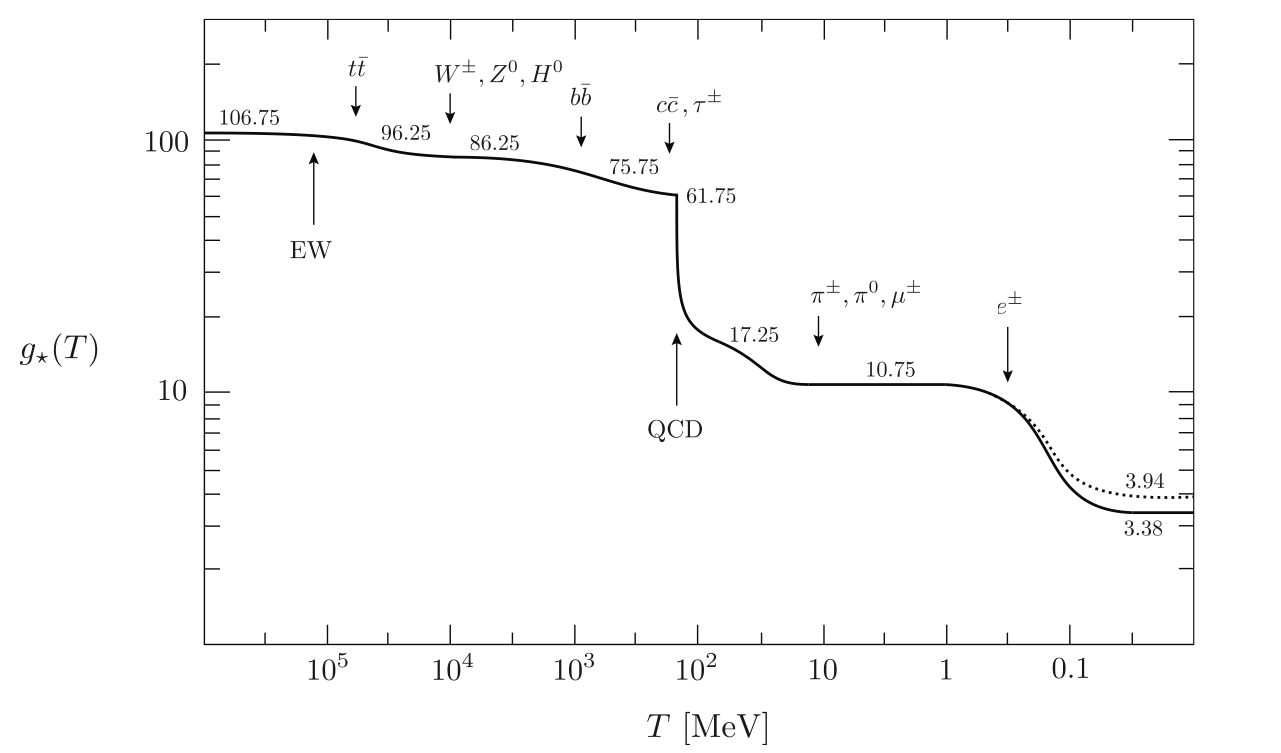
\includegraphics[width=\columnwidth]{Cosmology/gstar.png}
\end{center}
\caption{Effective number of relativistic degrees of freedom as a function of temperature. The numerical values are displayed before and after each phase transition. The solid line corresponds to $g_\star = g_{\star}^{\mathrm{th}} + g_{\star}^{\mathrm{dec}}$ whereas the dotted line corresponds to $g^s_{\star}$.}
\label{fig:gstar}
\end{figure}

The expansion of the Universe is often described as \emph{adiabatic}, which simply expresses that entropy is conserved, $dS / dT = 0$. The entropy density $s$ is defined as the sum of entropy densities of each species label by the index $\alpha$:
\begin{equation}
\label{eq:entropydensity}
s = \sum_{\alpha} \frac{\rho_{\alpha} + \mathcal{P}_{\alpha}}{T_{\alpha}} = \frac{2 \pi^2}{45} g^s_{\star} (T) T^3
\end{equation} where $g^s_{\star}$ is the effective number of degrees of freedom \emph{in entropy}. The entropy conservation assures that the entropy density scales as volume: $s \propto a^{-3}$, and so the temperature actually scales as $T \propto {g^s_\star}^{-1/3} a^{-1}$. Any relativistic species decoupling from the background photons alters the value of $g^s_\star$ and thus the evolution of the background temperature. Fig.~\ref{fig:gstar} recaps the value of $g_{\star}^{\mathrm{th}} + g_{\star}^{\mathrm{dec}}$ and $g^s_{\star}$ as a function of temperature.

\clearpage



	\section{The Energy Content of the Cosmological Fluid}
	\label{sec:inventory}
	\vspace*{1.5pc}

As the general relativity description of the spacetime metric historically engrained into the roots of modern observational cosmology, there was a divide as to the driving force responsible for the expansion. One school of thought put forth the \emph{steady state} model, in which the density of matter remains unchanged in the expanding Universe due to a steady homogenous creation of matter. The other school of thought, which would ultimatly prevail, proposed the \emph{Hot Big Bang} model, in which the matter density monotonically decreases as the scale factor increases. Consequently, the Universe was denser and hotter at earlier times, which I detailed in Sec.~\ref{sec:thermal}. In this section, I break down the main components of the cosmological fluid that obey Friedmann's equations. 


\subsection{Non Particular Components}

First shall be specified two components of the cosmological fluid that are not made of particles, but oddly have a defined energy density: the global curvature of the Universe and the cosmological constant. 

\subsubsection{Curvature}

From cosmological observation, it appears that the Universe has a global flat spatial geometry. Setting $\kappa=0$ in the first Friedmann equation defines the cosmological fluid's critical density $\rho_{\mathrm{cri}}$: \\
\begin{empheq}[box=\mymath]{equation}
\rho_{\mathrm{cri}}(t) = \frac{3H^2(t)}{8 \pi G}
\end{empheq} \\ with today's value being $\rho_{\mathrm{cri},0} = 8.293 10^{-11} h^2 ~\mathrm{eV}^4$ (see Appendix~\ref{apx:units} for expressing physical quantities in units of $h_p$, $k_b$ and $c$). In units of this critical density, the Friedmann equation can be written in compact form \\
\begin{equation}
\label{def:omega}
\rho(t) = \Omega(t) \times \rho_{\mathrm{cri}} (t)
\end{equation} \\ where the cosmological fluid is an admixture of radiation, non-relativistic matter and a curvature density \\
\begin{equation}
\rho_\kappa(t) = - \frac{3 \kappa}{8 \pi G} \frac{1}{a^2(t)}
\end{equation} \\ so that \\
\begin{equation}
\label{eq:rho_tot_def}
\rho(t) = \sum_{\alpha \in \lbrace r,m,\kappa \rbrace} \rho_\alpha (t) = \sum_{\alpha \in \lbrace r,m,\kappa \rbrace} \Omega_\alpha (t) ~ \rho_{\mathrm{cri}} (t)
\end{equation} \\ The curvature density is not a physical quantity. However, from Eq.~\ref{eq:rho_tot_def}, one can interpret it as the energy density that exceeds or is deficient with regards to the critical value that would make the Universe flat. In all that follows, I work under the assumption that $\kappa = 0$, and drop any contribution of $\rho_\kappa$ into Friedmann's equations.

\subsubsection{Dark Energy or Cosmological Constant}

Hubble diagrams of distant objects provided in the late 90's evidence for a negative value of the deceleration parameter $- \ddot{a}a/\dot{a}^2$, which appears under another normalisation as the second order term in Eq.~\ref{def:deva}. In other words, the expansion of the Universe was not decelerating as would be the case if the expansion was driven solely by the matter and radiation density; it was in fact doing just the opposite. \\

Because both the Einstein and metric tensors are divergencefree, one can incorporate a so-called \textbf{cosmological constant} $\Lambda$ into the Einstein tensor ($\pmb{G} \mapsto \pmb{G} - \Lambda \pmb{g}$) and verify the Einstein field equations: \\
\begin{equation}
\label{eq:EFE_contracted}
G_{\mu \nu} - \Lambda g_{\mu \nu} = 8 \pi G T_{\mu \nu}
\end{equation} \\ In this context, the $\Lambda$ scalar is uniform in space (although not necessarily in time) and acts as a ``drain'' term in spacetime warping. Another possible interpretation for the accelerated expansion of the Universe comes from incorportating it into the energy-stress tensor instead: $\pmb{T} \mapsto \pmb{T} + \Lambda \pmb{g}$, making it a ``source'' term in energy density, called \emph{dark energy}. In that case, this additional term can be thought of as a fluid whose equation of state is \\
\begin{empheq}[box=\mymath]{equation}
w_\Lambda = -1
\end{empheq} \\ In other words, the more you compress it, the less dense it gets. Inversely, as the Universe expands and the cosmological fluid dilates, the dark energy component exerts growing pressure on its surroundings and drives the expansion ever so further. It goes without saying that there are currently no known material on Earth displaying such a counter-intuitive property. It is still to this day unclear which of these two interpretations --- as a dark energy in $\pmb{T}$ or a cosmological constant in the EFEs --- is correct, if any one of them at all, since both of them involve a standing mystery as to its nature, behavior and origin. \\

\begin{figure}[!]
\begin{center}
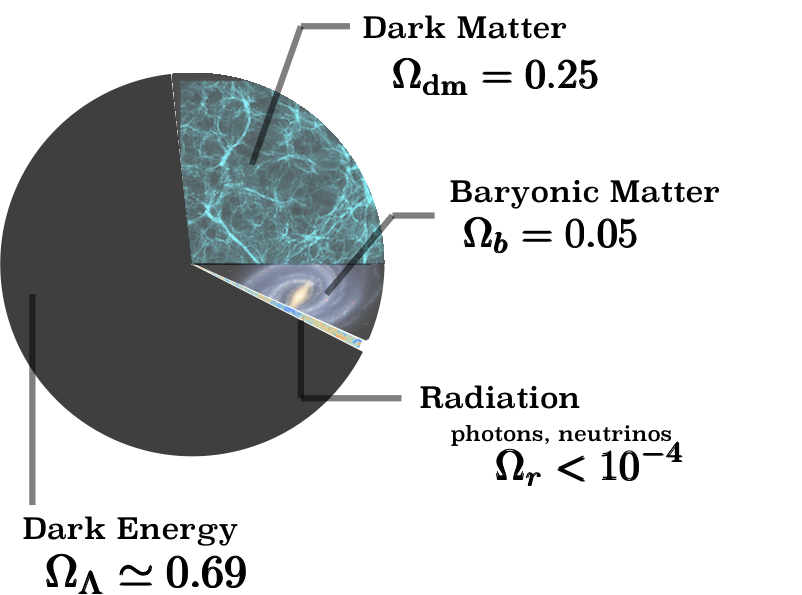
\includegraphics[width=0.65\columnwidth]{darkside.png}
\caption{Relative abundance in terms of energy density of the main components of the Universe today ($z=0$).}
\end{center}
\label{fig:camembert}
\end{figure}


The total energy density in units of critical density must therefore be written

\begin{equation}
\Omega_r + \Omega_m + \Omega_{\Lambda} = 1 - \Omega_{\kappa}
\end{equation} with $\Omega_\kappa = 0$ for a flat Universe. This expression introduces the quantity
\begin{equation}
\label{eq:rhode}
\rho_\Lambda = \frac{\Lambda}{8 \pi G}
\end{equation} which is derived from the Friedmann equations with Eq.~\ref{eq:EFE_contracted} as the expression of the EFEs. This quantity being homogenous to an energy density, it follows that in the cosmological constant interpretation of the acceleration of the Universe's expansion, $\Lambda$ has dimentions of the inverse of a surface. Several cosmological probes either measure independantly or infer $\Omega_\Lambda \sim 0.7$ today. Throughout this work, I used the value \\
\begin{empheq}[box=\mymath]{equation}
\label{eq:omega_lambda}
\Omega_\Lambda = 0.69
\end{empheq} \\ consistent with the best fitted value from the Planck collaboration's analysis on the cosmic microwave background temperature anisotropies. Notice from Eq.~\ref{eq:rhode} that the energy density associated with $\Lambda$ (or dark energy, which I'll use interchangeably throughout this thesis) is only implicitely dependant on time through $\Lambda$'s own time dependance. In the benchmark cosmological model, $\Lambda$ is deemed a constant in both space and time, and so $\rho_\Lambda \propto a^0$. In a $\Lambda$ dominated Universe, which applies to the current state of the Universe, the first Friedmann equation simplifies to \\

\begin{equation}
\label{eq:Friedmann_LDE}
\left( \frac{\dot{a}}{a} \right)^2 \simeq \Omega_\Lambda
\end{equation} \\ which integrates into $a(t) \propto \exp\left[ H_0 \Omega_\Lambda^{1/2} t \right]$, or, using conformal time, $a(\tau) \propto (-\tau)^{-1}$.

\subsection{Inventory of Radiation}
\label{sec:radiation}

With the non-particular components of the cosmological fluid out of the way, we can instantiate the relativistic matter population, which in sum total has an energy density of

\begin{empheq}[box=\mymath]{equation}
\label{eq:omega_radiation}
\Omega_{r,0} = 8.24 \times 10^{-5}
\end{empheq} \\ critical densities. The only relativistic species today are (1) photons from the cosmic microwave background, (2) massless\footnote{by massless I mean any neutrino mass eigenstate lighter than $10^{-4}~\mathrm{eV}$} neutrinos from the cosmic neutrino background, and (3) any hypothetical light thermal relic; all three of which I detail in the subsections below.


\subsubsection{The Cosmic Microwave Background}

\begin{figure}
\begin{center}
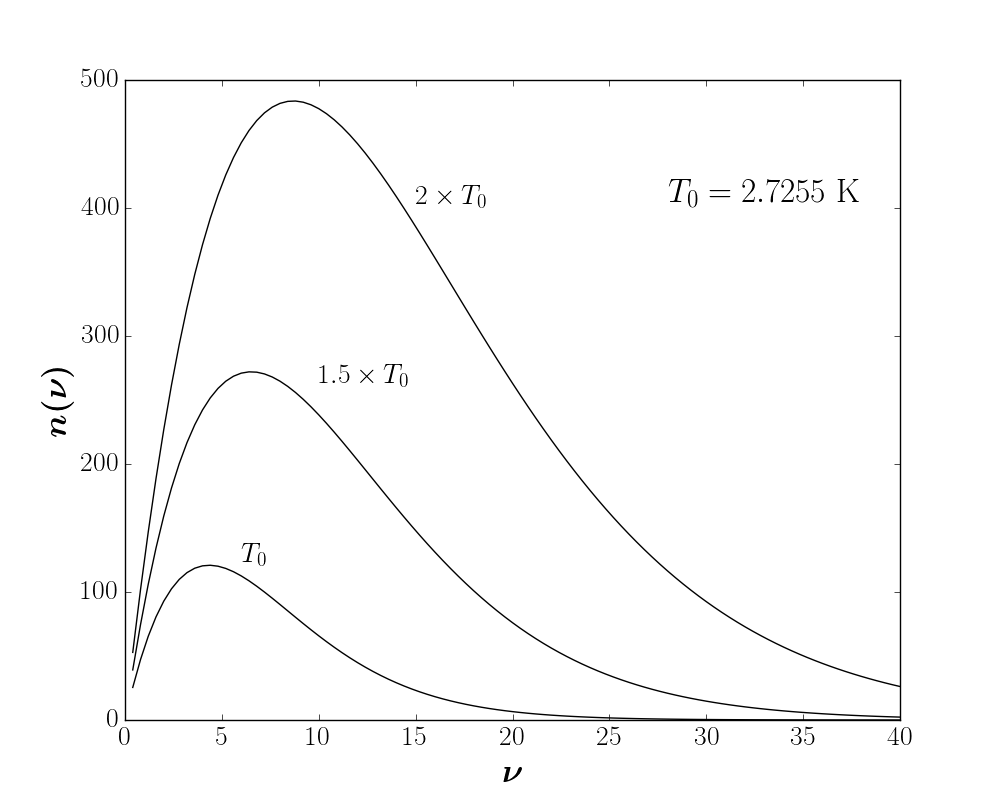
\includegraphics[width=0.75\columnwidth]{photon_eq.png}
\caption{energy density per unit of frequency of photons in thermal equilibrium as a function of frequency given by Eq.~\ref{eq:Fermi_photon} for 3 temperatures. Units are arbitrary.}
\label{fig:planck_eq}
\end{center}
\end{figure}

Up until recombination, the rate of expansion was significantly weaker than the scattering interaction rate between photons and free electrons $H(t) \ll \Gamma_{\mathrm{Compton}}$. This thermal equilibrium defines its black body temperature $T_\gamma$. Since photons have no chemical potential, 
\begin{equation}
\label{eq:Fermi_photon}
n_{\gamma} (E) dE \propto \frac{E^2 dE}{e^{E / k_b T_\gamma} - 1}
\end{equation} with $dE = h d\nu$ the energy interval and $\nu$ the photon frequency. The energy density of photons is therefore proportional to the 4th power of its black body temperature, known as \emph{Stefan's Law} \\
\begin{equation}
\label{eq:photon_rho}
\rho_\gamma c^2 = \int_0^\infty E dE~n(E) = \frac{8 \pi^5}{15} \frac{k_b^4}{15 h^3 c^3} ~ T_\gamma^4
\end{equation} \\ which is conformal to the expression in Eq.~\ref{eq:relmat} for bosons with $g=2$ (there are two spin states). The energy of a photon is inversely proportional to its wavelength $\lambda = \hbar c / k_b T_\gamma \propto a(t)$ which scales as the scale factor. This implies that the evolution of temperature with the scale factor is 
\begin{equation}
\label{eq:T_f_a}
T(t) = \frac{T_0}{a(t)}
\end{equation} As the Universe expands, the energy density of photons is therefore diluted by this $a^{-1}$ factor pertaining to its energy in addition to the $a^{-3}$ factor pertaining to the dilution of volume, as illustrated in Fig.~\ref{fig:expa}. At any point in time $t$, the energy density is therefore \\

\begin{equation}
\label{eq:rho_photon_f_a}
\rho_\gamma (t) = \rho_\gamma^0 ~\left( \frac{a_0}{a(t)} \right)^4
\end{equation} \\ with $\rho_{\gamma, 0}$ its current value. \\

As the background temperature falls below the binding energy of the Hydrogen atom, electrons progressively bound to protons. Once recombination is complete, because of global neutrality, there are too few free electrons for photons to scatter off and they free-stream with a mean free path of $c/H(t)$ in the direction of their last scattering event. Photons are no longer in thermal equilibrium but their black body distribution of Eq.~\ref{eq:Fermi_photon} freezes-out and imprints their former equilibrium spectrum since they effectively do not interact with any species along their path. As Fig.~\ref{fig:planck_eq} displays, the photon's energy density distribution retains its black body spectrum as if it were in equilibrium. As the Universe expands, the temperature falls as $T_\gamma \sim a^{-1}$ which redshifts the $T(t_{\mathrm{LSS}}) \sim 13.6 ~\mathrm{eV}/k_b$ of these last scattered photons to microwaves today $T_0 \sim 2.35 \times 10^{-4} ~\mathrm{eV}/k_b = 2.7255 ~\mathrm{K}$. The black body spectrum measured today is known as the Cosmic Microwave Background (CMB) radiation. The current value of their energy density is obtained by setting $T_\gamma = T_{\gamma, 0}$ in Eq.~\ref{eq:photon_rho}, which yields $\rho_{\gamma, 0} c^2 = 0.2606~\mathrm{MeV}$ in units of $k_b^4\hbar^{-3}c^{-3}$; or, in units of critical density: \\

\begin{empheq}[box=\mymath]{equation}
\Omega_{\gamma, 0} \simeq 5.35 \times 10^{-5}
\end{empheq} \\

From the measured redshifting of CMB photons, one can trace back the last scatterings to having occured when the scale factor was approximately a thousand times smaller than today. Recombination is not an instantaneous process and the distribution of electrons was not perfectly homogenous at the time of the so-called \textit{decoupling} of electrons and protons from thermal equilibrium. Therefore small departures or fluctuations from the black body spectrum are expected in the energy distribution of CMB photons today. These temperature fluctuations serve as a powerful tool to probe inhomogeneities and anisotropies in the distribution of matter at $z \sim 1,050$ (some $\sim 380,000$ Gyr after the big bang). Current measurements of these temperature fluctuations show they are of the order $\theta = \delta T / T \sim 10^{-5}$. This will justify treating temperature perturbations in the next chapter as being linear.\\


\subsubsection{The Cosmic Neutrino Background}

In the early Universe, neutrinos are kept in thermal equilibrium as long as the rate of weak interactions ($e^{-} + e^{+} \rightleftharpoons \nu_e + \bar{\nu}_e$) outdoes the rate of expansion. The energy distribution also follows a Fermi distribution which defines for each neutrino species a temperature $T_\nu$ such that
\begin{equation}
\label{eq:Fermi_neutrino}
n_{\nu} (E) dE \propto \frac{E^2 dE}{e^{(E - \mu) / k_b T_\nu} + 1}
\end{equation} with $\mu$ the chemical potential. Under the assumption net lepton symmetry in the early Universe, Eq.~\ref{eq:Fermi_neutrino} holds for both neutrinos and anti-neutrinos of each lepton charge, since in that case $\mu_{\bar{\nu}} = 0 = - \mu_\nu$. Each generation of neutrino freezes out of thermal equilibrium consecutively when the temperature $T$ was such that
\begin{equation}
\Gamma = n \langle \sigma v \rangle \sim G^2_\mathrm{F} T^5 \sim \sqrt{G_\mathrm{N} T^4} \sim H
\end{equation} where $G_\mathrm{F}$ and $G_\mathrm{N}$ are the Fermi and Newton constants. Electron neutrinos for instance, which decouple last, do  so when $T \sim 1 ~\mathrm{MeV}$. Shortly after, at $T \sim 0.5 ~\mathrm{MeV}$, $e^{\pm}$ annihilation is favoured over pair production. Assuming neutrinos were completely decoupled, they remained at that temperature while the entropy release heated the CMB photons by a factor $(11/4)^{1/3} \simeq 1.401$. 
This factor comes from the conservation of the entropy density (see Eq.~\ref{eq:entropydensity} and Fig.~\ref{fig:gstar}) while the Universe expands adiabatically, assuming that all the entropy released from the $e^{\pm}$ annihilation all transfered instantaneously into the photons, which equates\\
\begin{equation}
\left[ g_\star T^3\right]_\mathrm{before} = \left[ g_\star T^3\right]_\mathrm{after}
\end{equation} \\ where $g_\star^\mathrm{after} = 2$ because photons are massless fermions, while $g_\star^\mathrm{before} = 5.5$ before annihilation because there are an additional $2 \times 7/8$ degrees of freedom for electrons, and another for positrons since both are fermions. \\

Like photons, once neutrinos decoupled, their energy distribution retained the shape of a black body spectrum\footnote{with regards to the Fermi distribution, not a Bose distribution to which the black body description applies} with decreasing temperature $T_\nu \propto a^{-1}(t)$. Consequently, after their decoupling, neutrinos are throughout conformal times about $40\%$ cooler than CMB photons: \\
\begin{equation}
T_\nu = \left( \frac{4}{11} \right)^{1/3} T_\gamma
\end{equation} \\ Today, the Cosmic Neutrino Background (CNB) has cooled to $T_{\nu,0} = (4/11)^{1/3} T_\gamma^0 = 1.9525 ~\mathrm{K}$. Currently, each generation of neutrino -- antineutrino pair has an energy density of \\
\begin{equation}
\rho_{\nu,0} c^2 = \frac{7}{8} \frac{\pi^2}{15} \frac{k_b^4}{\hbar^3 c^3} \times T^4_{\nu, 0}
\end{equation} \\ in the massless approximation. The total massless neutrino energy density in units of critical energy density is therefore \\

\begin{empheq}[box=\mymath]{equation}
\Omega_{\nu,0} = 1.25 \times 10^{-5} \times N_\nu
\end{empheq} \\ where $N_\nu = 3$ is the number of lepton charged neutrinos and their associated antineutrinos. 
Because of lepton charge oscillations in neutrinos, we know that not all three mass eigenstates are massless, and neither are the $\nu_{e, \mu, \tau}$. We thus expect a departure from this $N_\nu = 3$ value, which assumes their energy density follows Stephan's Law $\rho_\nu \propto T_\nu^4$ like any radiation (modulo the $7/8$ factor for their fermionic nature). In this approximation, the mass only intervenes via its temperature\footnote{since its energy is the sum of its rest mass energy and its kinetic (thermal) energy}. As such, a $m^{\mathrm{eff}}_\nu = 93.14~\mathrm{eV}$ neutrino would have critical energy density assuming $H_0 = 100~ \mathrm{km}~s^{-1}\mathrm{Mpc}^{-1}$. In other words, neutrinos contribute
\begin{equation}
\label{eq:omnu}
\Omega_\nu h^2 = \frac{m^{\mathrm{eff}}_\nu}{93.14~\mathrm{eV}}
\end{equation} to the total energy density of a flat Universe. Furthermore, neutrino freeze-out is not an instantaneous process. A portion of neutrinos are still coupled to photons as electrons and positrons pair-annihilate and heat the CMB photons. As a result, this correction is incorporated into the \emph{effective} number of neutrino species (neutrino and antineutrino) $N_\mathrm{eff} = 3.046$ which would be 3 in the approximation of instantaneous decoupling of neutrinos from photons. The correct expression for the neutrino energy density is therefore

\begin{equation}
\begin{array}{lcl}
\cfrac{\rho_\nu}{\rho_\gamma} & = & \cfrac{7}{8} N_{\mathrm{eff}} \times \left( \cfrac{T_\nu}{T_\gamma} \right)^4 \\
& & = \cfrac{7}{8} \left( \cfrac{4}{11} \right)^{4/3} N_{\mathrm{eff}}
\end{array}
\end{equation}

%\begin{align*}
%\frac{\rho_\nu}{\rho_\gamma} & = \frac{7}{8} N_{\mathrm{eff}} \times \left( \frac{T_\nu}{T_\gamma} \right)^4 \\
%& = \frac{7}{8} \left( \frac{4}{11} \right)^{4/3} N_{\mathrm{eff}}
%\end{align*}

\subsubsection{Extra Radiation}
\label{sec:extrarad}

The combined TT+TE+EE+lowP Planck analysis \citep{Planck2015} of the CMB temperature anisotropies constrain the effective number of stable, relativistic species in thermal equilibrium in the early Universe to \\
\begin{equation}
\label{eq:neff_cmb}
N_{\mathrm{eff}} = 2.99 \pm 0.20
\end{equation} \\

As apparent in Fig.~\ref{fig:gstar}, neutrinos aren't the only fermions aside from baryons to be coupled to photons as some point during the early Universe. Any particle of mass $m_x$ and temperature $T_x$ coupled to photons prior to neutrino decoupling would contribute an additional $\Delta N_{\rm{eff}} \propto (T_x/T_\nu)^4$ to the effective number of neutrinos, where 
\begin{equation}
N_{\mathrm{eff}} = 3.046 \pm \Delta N_{\mathrm{eff}}
\end{equation} These \textbf{early-decoupled thermal relics} as they are generically refered to, have momentum distributions that obey Fermi-Dirac statistics while in equilibrium, as per Eq.~\ref{eq:Fermi_neutrino}. However, their temperature may differ from the neutrino temperature. If one assumes dark matter is made of these early-decoupled thermal relics, then setting $\Omega_x = \Omega_{\mathrm{dm}}$ fixes the departure from $N_{\mathrm{eff}}$ via

\begin{equation}
\label{eq:omx}
\frac{m_\nu^{\mathrm{eff}}}{m_x} = \left( \frac{T_x}{T_\nu} \right)^3 = \left( \Delta N_{\mathrm{eff}} \right)^{3/4}
\end{equation} \\ with $m_\nu^{\mathrm{eff}}$ introduced in Eq.~\ref{eq:omnu}. The total radiation energy density can therefore be expressed as a factor of $\rho_\gamma$ through $N_{\mathrm{eff}}$ and its departure from $3.046$:

\begin{equation}
\begin{array}{ll}
\rho_r & = \rho_\gamma + \rho_\nu + \rho_x \\
 & = \rho_\gamma + \cfrac{7}{8} \left( \cfrac{4}{11} \right)^{4/3}~N_{\mathrm{eff}}~\rho_\gamma + \cfrac{7}{8} \left( \cfrac{4}{11} \right)^{4/3}~\Delta N_{\mathrm{eff}}~\rho_\gamma \\
 & = \rho_\gamma \times \left[ 1 + \cfrac{7}{8}\left( \cfrac{4}{11} \right) ^{4/3} ~\left( N_{\mathrm{eff}} + \Delta N_{\mathrm{eff}} \right) \right]
\end{array}
\end{equation} \\ where the left-hand, middle and right-hand terms are respectively the photon, thermalized (left-handed) neutrinos and all extra radiation, \textit{i.e.} either thermalized relics or neutrinos which haven't reached thermal equilibrium, which I detail in Sec.~\ref{sec:rhneu} below.


\subsubsection{Sterile Neutrinos}
\label{sec:rhneu}

The constraints on $N_{\mathrm{eff}}$ (Eq.~\ref{eq:neff_cmb}) rule out $N_\nu = 4$ at the $\sim 5\sigma$ level. This means that if right-handed neutrinos exist, then they must not have reached thermal equilibrium with photons. There are several ways hypothetical sterile neutrinos could have been produced in the Early Universe. Because of their coupling to lepton-charged neutrinos, right-handed neutrinos can be produced \textit{e.g.} via the oscillation mechanism from an ``active'' mass eigenstate to a sterile one. \cite{DodelsonWidrow94} showed that this production by oscillation reaches maximum efficiency when $T \sim 0.1-0.3~\mathrm{GeV}$. These sterile neutrinos are not in thermal equilibrium with photons, in fact they do not interact at all. However, since the distribution of the active states are Fermi-distributed, it is expected that the distribution function of the sterile states $f_s$ closely resemble one as well:
\begin{equation}
\label{eq:fs}
f_{s} \propto \frac{\vartheta}{e^{(E-\mu_s)/T_\nu}+1}
\end{equation} where the rescaling factor $\vartheta = \Delta N_{\mathrm{eff}} = \sin^2 2 \theta \ll 1$ is related to the active-sterile angle $\theta$. The DW neutrino assumes that the effective massless degree of freedom $g_\star$ is constant at $T \sim 100~\rm{MeV}$, but as \cite{Abazajian2016} point out, this isn't the case, and even less so the actual relevant quantity  $d \ln g_\star / d \ln a$. Incorporating this contrast with the idealized DW case and making no assumptions on the initial abundances, \cite{Merle_DW} show that the Boltzmann equation can be written as
\begin{equation}
	\left[ \frac{\partial}{\partial T} - \kappa(T) p~ \frac{\partial}{\partial p} \right]~ f_s (p, T) = \mathcal{H}(p,T) \times \left[ f^{\mathrm{DW}}_s - f_s \right](p,T)
		\label{eq:Merle}
\end{equation} where $\kappa(T)dT = H(T)dt$ and the $\mathcal{H}$ function generically encapsulates all thermodynamics and production processes involved. Since $\mathcal{H}$ varies rather dramatically with neutrino momentum $p$, sterile neutrinos produced in oscillations do not feature a re-scaled thermal distribution as is commonly assumed. To distinguish them from the idealized DW case, we refer to neutrinos produced in this mechanism as \textbf{non-resonant}; or NRP\footnote{for ``non resonantly produced''} sterile neutrinos. Readers should keep in mind that the actual distribution of NRP $\nu_s$ has lower momenta than DW $\nu_s$, as is shown in Fig. 1 of \cite{Merle_DW}. The NRP $f_s$ is characterized by the integral over temperature of $\mathcal{H}$, which is close to unity to a few percent. In this work, I limit the analysis of neutrino dark matter to Ly-$\alpha$ forests, which only requires an accuracy at the percent level. In this context, it is therefore adequate to make the simplifying assumption that the $\mathcal{H}$ temperature integral is $\sim 1$ and that the contrast between the quasi-thermal DW distribution and the cooler NRP distribution is negligeable in the scope of my work.  \\

\begin{figure}
\begin{center}
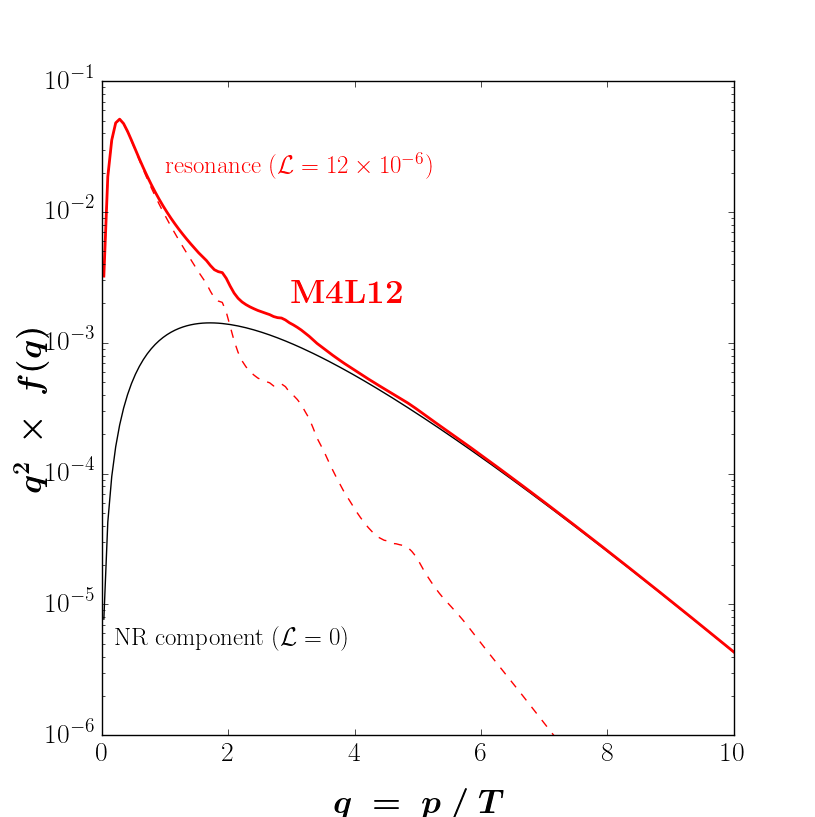
\includegraphics[width=0.55\columnwidth]{RPSN/RPSN_M4L12_psd.png}~%
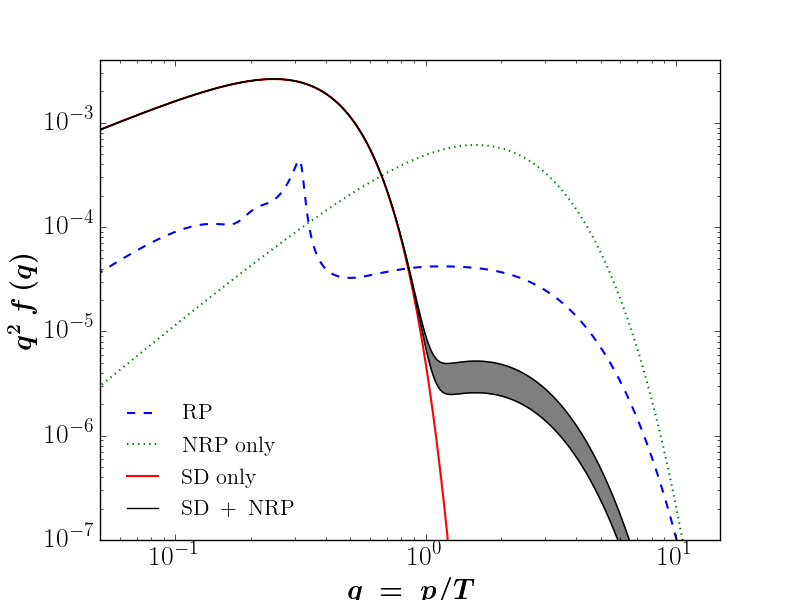
\includegraphics[width=0.55\columnwidth]{RPSN/SD.png}
\caption{\textbf{Left:} Distribution function of a $m_{\nu_s} = 4~\mathrm{keV}$ sterile neutrino produced via oscillations in presence of a net lepton asymmetry of $\mathcal{L} = 1.2 \times 10^{-5}$ (red solid curve labeled `M4L12'). The purely resonant component is featured in dashed red to distinguish it from the non-resonant component in solid black. \textbf{Right:} Distribution functions of $m_{\nu_s} = 7.1~\mathrm{keV}$ sterile neutrinos produced non-resonantly (dotted green curve labeled `NRP'), resonantly (dashed blue curve labeled `RP') and by the decay of a scalar field (red and black solid curves).}
\label{fig:M4L12_fs}
\end{center}
\end{figure}


As \cite{ShiFuller99} point out, the production of right-handed neutrinos via oscillations with the left-handed ones can be significantly boosted if one assumes a net lepton asymmetry in the Early Universe. The chemical potential term $\mu > 0$ in Eq.~\ref{eq:fs} can reach orders of $\mu \sim 10^{-4}$. The resulting distribution function of these \textbf{resonantly produced sterile neutrions} (RPSN) can end up being highly non-thermal, such as the one featured in red on the left panel of Fig.~\ref{fig:M4L12_fs} (also the dashed blue curve on the right panel ), produced in presence of a net lepton\footnote{I assume the lepton asymmetry to be mainly of the electronic charge, although there may be muonic and tauic charge asymmetries as well.} asymmetry of $\mathcal{L} = 1.2 \times 10^{-5}$ where $\mathcal{L}$ is the numerical density asymmetry of electronic neutrinos in units of entropy density:
\begin{equation}
\mathcal{L} = \frac{\left\vert n_{\nu_e} - n_{\bar{\nu}_e} \right\vert}{s}
\end{equation} To be consistent with light element abundances from big bang nucleosynthesis (BBN), this electronic asymmetry cannot exceed $\mathcal{L} \sim 10^{-3}$. However, asymmetries 3 orders of magnitude fainter than that upper limit can produce a significant resonance peak manifest in the distribution functions of RPSN. As such, RPSN are distributed with lower momenta than the quasi-thermally distributed NRP sterile neutrinos. If one assumes these neutrinos make up the dark matter, or part of it, then one can produce them with much weaker interaction angles $\theta$ for a fixed $\Omega_{\nu_s} \sim \Omega_{\mathrm{dm}}$ compared to Eq.~\ref{eq:fs}. \\

In this thesis, I consider left-handed and right-handed neutrinos as dark matter candidate particles. For the latter, I only consider ones produced via the oscillation mechanism, either in presence or absence of a net lepton asymmetry at the era of peak production. It should be noted, nevertheless, that ample other production mechanisms exist, which can all yield non thermal distributions typically cooler than the NRP case. Aside from the aforementioned NRP and RP production, neutrinos can be produced by the \textbf{decay of a scalar field}, initially proposed by \cite{Scalar_Decay3} and investigated by \cite{Scalar_Decay1, Scalar_Decay2, Scalar_Decay4}. The first numerical results were produced by \cite{Scalar_Decay_Merle}. The right panel of Fig.~\ref{fig:M4L12_fs} features the excess of momenta states populated in this production mechanism, where the position of the peak is linked to the scalar field particle's mass. Another noteworthy production mechanism is \textbf{thermal overproduction} with a subsequent entropy dilution, first put forth by \cite{thermal_overproduction} and reviewed in \cite{KingMerle}. The object of my thesis isn't to explore the plethera of production mechanisms, however, and I limit this current discussion to only the main axes of research on this topic. \\

Regardless of the production mechanism, the integral of the distribution function over all momenta yields the departure from the effective number of stable relativistic thermalized species in the early Universe from its fiducial value of $N_{\mathrm{eff}} = 3.046$: \\
\begin{equation}
\int \frac{dq}{2 \pi^2} q^2 f_s (q) = \frac{7}{8} \frac{\pi^2}{15}~T^4_\nu~\Delta N_{\mathrm{eff}}
\end{equation} \\To be consistent with the currently allowed bound on $N_{\mathrm{eff}}$ in Eq.~\ref{eq:neff_cmb}, the value of the normalisation parameter $\vartheta$ of the NRP sterile neutrinos' distribution function in Eq.~\ref{eq:fs} must not be of order unity. Typically, $\vartheta = \sin^2 2 \theta \simeq 10^{-7}$ for a NRP sterile neutrino of rest mass $m_{\nu_s} \sim \mathrm{keV}$ can account for $\Omega_{\mathrm{dm}} \simeq 0.26$ (see Sec.~\ref{sec:dmintro}). For a RPSN of the same mass, $\vartheta \simeq 10^{-12}$ can yield that same energy density and the same $\Delta N_{\mathrm{eff}}$. 








\subsection{Inventory of Non-Relativistic Matter}

I now instantiate the non-relativistic matter population, which in sum total have an energy density of \\
\begin{empheq}[box=\mymath]{equation}
\label{eq:omega_matter}
\Omega_{m} = 0.26142
\end{empheq} \\ critical densities today, and are subdivided into three categories: (1) everything made of atoms, including stars, dust and gas, (2) everything that has mass but isn't made of atoms, \emph{dark matter}, and (3) black holes. Leaving aside the third category, I detail the first two in the following two subsections. When matter is the dominant component in terms of energy density, then the first Friedmann equation boils down to:\\

\begin{equation}
\label{eq:Friedmann_MDE}
\left( \frac{\dot{a}}{a} \right)^2 \simeq \Omega_m = \Omega_{m,0} ~a^{-3}
\end{equation} \\ which integrates into $a(t) \propto t^{2/3}$ or equivalently $a(\tau) \propto \tau^{2}$ in terms of conformal time.


\subsubsection{Baryons and Acoustic Oscillations}
\label{sec:baos}

\begin{figure}
\centering
\begin{subfigure}{0.49\textwidth}
\centering
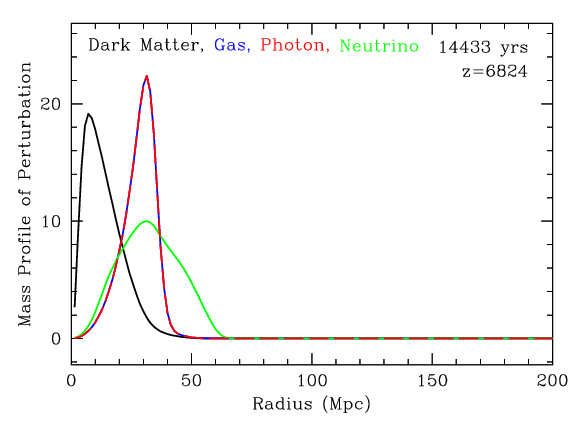
\includegraphics[width=\textwidth]{BAO/bao_z6824.png}
\caption{Near the initial time, the photons and baryons travel outward as a pulse.}\label{fig:bao_z6824}
\end{subfigure}
\hfill
\begin{subfigure}{0.49\textwidth}
\centering
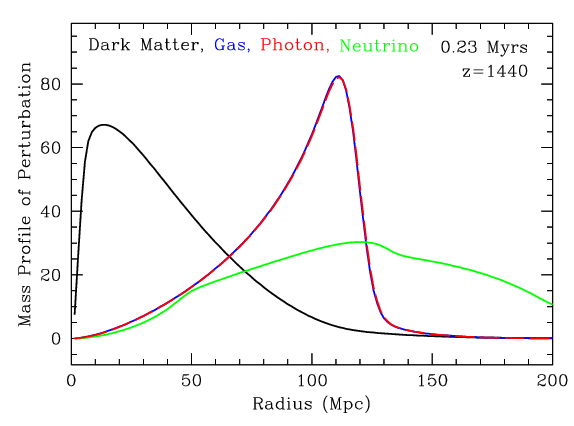
\includegraphics[width=\textwidth]{BAO/bao_z1440.png}
\caption{Approaching recombination, one can see the wake in the cold dark matter raised by the outward-going pulse of
baryons and relativistic species.}\label{fig:bao_z1440}
\end{subfigure}

\begin{subfigure}{0.49\textwidth}
\centering
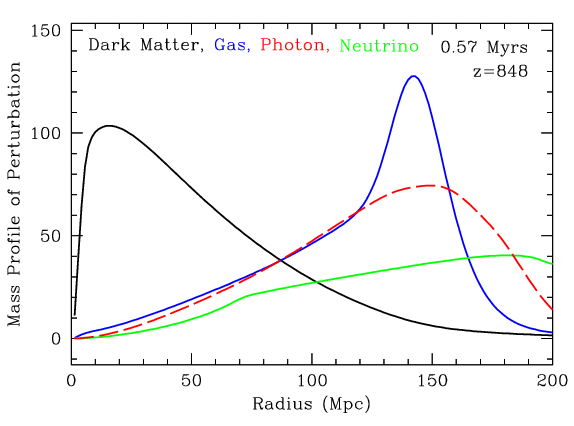
\includegraphics[width=\textwidth]{BAO/bao_z848.png}
\caption{At recombination, the photons leak away from the baryonic perturbation.}\label{fig:bao_z848}
\end{subfigure}
\hfill
\begin{subfigure}{0.49\textwidth}
\centering
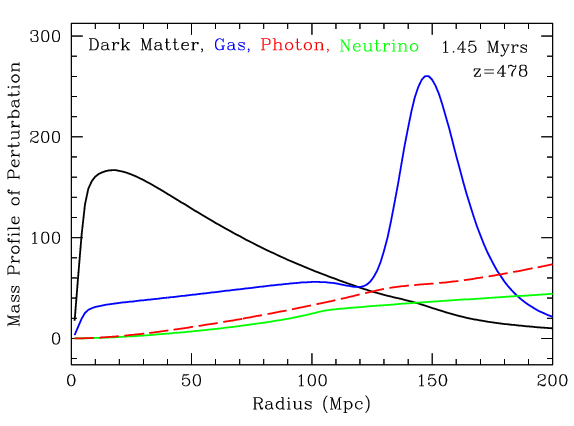
\includegraphics[width=\textwidth]{BAO/bao_z478.png}
\caption{With recombination complete, we are left with a dark matter perturbation toward the center and a baryonic
perturbation in a shell.}\label{fig:bao_z478}
\end{subfigure}

\begin{subfigure}{0.49\textwidth}
\centering
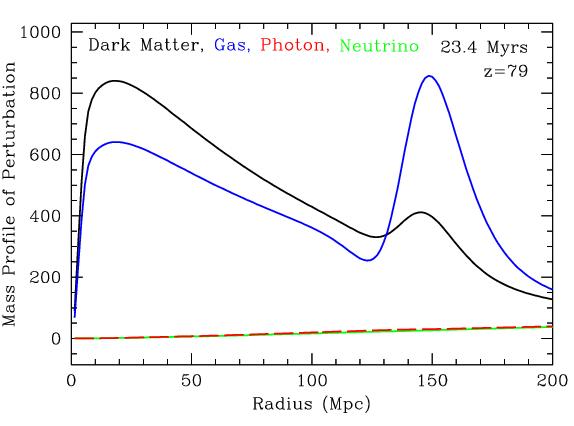
\includegraphics[width=\textwidth]{BAO/bao_z79.png}
\caption{Gravitational instability now takes over, and new baryons and dark matter are attracted to the overdensities.}
\label{fig:bao_z79}
\end{subfigure}
\hfill
\begin{subfigure}{0.49\textwidth}
\centering
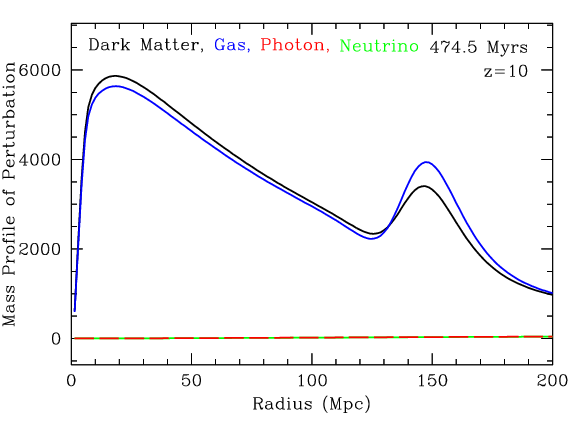
\includegraphics[width=\textwidth]{BAO/bao_z10.png}
\caption{The gas and dark matter peaks now look alike. The acoustic peak has decreased in contrast because dark matter,
which has no peak initially, outweighs the gas.}\label{fig:bao_z10}
\end{subfigure}

\caption{Evolution of the radial fractional mass profile versus comoving radius of an
initially pointlike overdensity located at the origin. The units of the mass profile are arbitrary but are correctly scaled between the 
panels. These figures were made by suitable transforms of the transfer functions created by \texttt{CMBFAST} \citep{Seljak1996, 
Zaldarriaga2000}. Credits: \citet{Eisenstein2007}.}\label{fig:bao_propagation}
\end{figure}

To distinguish ``regular'' matter from dark matter, any system made of atoms is refered to as \textbf{baryons}. Today, an obvious amount of baryons are bound to gravitational systems such as stars, planets, \textit{etc} due to growing density perturbations on very small scales. At larger scales, the interstellar and intergalactic media consist of hot tenous plasma containing a substancial amount of baryons from neutral atoms to ionized molecules. At earlier times, when the Universe was denser and hotter, the distribution of matter and baryons was much more uniform. When the Universe cools down to the binding energy of Hydrogen, electrons increasingly bind to protons to form neutral Hydrogen and photons scattering off the remaining free-electrons decreasingly. This \emph{recombination} occurs at around $z_{\mathrm{rec}} \simeq 1100$. Once about $90\%$ of the electrons are bound in neutral Hydrogen, photons last scatter off their ultimate free electron before free-streaming out and making the Universe transparent. At the redshift of this last scattering surface, $z_{\mathrm{lss}} \sim 1050$, the distribution of baryons is homogenous to within $\sim 10^{-5}$. The theory of structure formation relies mainly on gravitational instability, that is, the idea that in overdense regions, gravitational collapse overcomes the expansion. Thus overdensities tend to grow over time. In underdense regions on the other hand, the expansion is preponderant over their self-gravity and as such grow more underdense over time. \\

Before recombination, Thomson scattering between photons and electrons is predominant and the free-streaming scale of photons is much smaller than the size of the horizon $c H^{-1}(z)$. Photons and electrons are thus strongly coupled. This is known as the \emph{strong coupling limit}. In addition, protons and electrons interact through the Coulomb force. These three types of particles are coupled and form a unique
fluid called the baryon-photon plasma in which density perturbations evolve like sound waves. A point-like adiabatic perturbation in this baryon-photon plasma affects the dark matter, baryon, photon and neutrino populations. Neutrinos interact very weakly and stream away from the initial perturbation due to their high velocity. Dark matter is only affected by gravity and thus only stands growing at the original position. Because the baryon-photon plasma is
very hot and dominated by photons at this time, it has a strong pressure compared to its density. The initial overdensity is thus
also an initial overpressure. As the pressure tries to equalize itself with its surroundings, this results in an expanding spherical
sound wave, or \textbf{acoustic oscillation}, with the sound speed in the plasma $c_s \simeq c / \sqrt{3}$. The baryon and photon perturbation is carried outwards and its density drops as the energy is spread over the expanding
spherical wave as shown in Fig~\ref{fig:bao_z6824}. \\

As the acoustic wave propagates, the neutrinos free stream out and dark matter accumulates in the overall density
perturbation. Not only is the DM peak growing, but the width of the perturbation widens since it attracts additional material from its surroundings. This can be seen in Fig.~\ref{fig:bao_z1440}. Once recombination onsets, baryons decouple from the photons. The tight coupling limit is no longer valid and photons free stream like the neutrinos initially did at the onset of the perturbation, as shown on Fig.~\ref{fig:bao_z848}. Photons cool down and their pressure drops as the decoupling occurs, and thus the acoustic wave decelerates. This process continues until the photons have completely leaked out of the perturbation, and the sound wave has almost stopped
propagating. The remnants are a dark matter perturbation around the origin and a gas perturbation in a shell of about $\sim 150~\mathrm{Mpc}$ (comoving), seen in Fig.~\ref{fig:bao_z478}. However, baryons and dark matter interact gravitationally thus causing the two perturbations to feedback, \textit{i.e.} both increase due to the combined gravitational potential from both components (see Fig.~\ref{fig:bao_z79}). Eventually, the two perturbations look scarcely dissimilar and the spherical shell of gas has imprinted itself in the dark matter as the so-called acoustic peak (Fig.~\ref{fig:bao_z10}). \\

Since these perturbation are small in amplitude, the process just described can be linearly summed over the whole set of perturbation in the baryon-photon plasma. Galaxy formation occurs in overdense regions, and although most of it happens at the position of the original fluctuations, there is a tiny excess in the $\sim 150~\mathrm{Mpc}$ regions away from these initial perturbations. This length scale, originally related to a density
excess shortly after recombination, is expected to also be present in the distribution of matter in the later universe. It can
therefore be used as a standard ruler to probe our cosmological model. This is detected as a single \emph{acoustic peak} in the
correlation function of galaxies or a series of \emph{acoustic oscillations} in the corresponding power spectrum
\citep{Eisenstein2005,  Anderson2012}. Using this BAO scale and CMB anisotropies, we know baryons contribute \\
\begin{empheq}[box=\mymath]{equation}
\Omega_{b} h^2 = 0.022
\end{empheq} \\ to today's critical energy density.

\subsubsection{Dark Matter}
\label{sec:dmintro}

At the beginning of the 20th century, there appeared to be less light emaning from gravitationally-bound star clusters orbiting distant nebul{\ae}. Initially thought of as a ``missing light'' problem in which some material obstructed or occulted the light from these background sources, it became apparent a few decades later that it was in fact a ``missing mass'' issue. Indeed, if clouds of gas or dust in the foreground had absorbed the incoming light, then it should have manifested radiating as a black body at some wavelength. The mass from these luminous sources only accounted for one fifth of that required for these systems to be gravitationally bound and to reproduce their velocity dispersions. The other missing four fifths were hypothesized as an additional Dark Matter (DM), that has mass but neither absorbs nor emits nor scatters off light. In other words, dark matter is very little if at all sensitive to the electromagnetic interaction. \\

Although bold at the time, the postulation for the existence of dark matter has thus far stood the test of time. Other independant observations infer its presence: the non-Newtonian rotation curves of galaxies for one, but also the anisotropies in CMB temperatures, the BAOs described in the previous subsection, and gravitational lensing pictured in the right panel of Fig.~\ref{fig:bullet}. None of them outright prove its existence. However, dark matter neatly explains these independant observations. Ever since the advent of computational astrophysics in the 80's, numerical simulations have been unable to correctly reproduce the formation of structures and galaxies with ``ordinary'' matter only. All of the aforementioned cosmological probes for dark matter point to it having \\
\begin{empheq}[box=\mymath]{equation}
\Omega_{\mathrm{dm}} h^2 = 0.119
\end{empheq} \\ of today's critical energy density. Its nature however, is still unknown. If it is made of elementary particles, then images like the one in the left panel of Fig.~\ref{fig:bullet} suggest it can't be baryonic matter. When two galaxy clusters collide, the gas heats and radiates in the X-ray part of the spectrum, pictured as the pink overlay. The blue overlay points to where most of the mass distribution lies, as deduced by the gravitational lensing it exerts on the background light (an example of strong gravitational lensing is provided on the right panel). The pink and blue regions are clearly disparate, suggesting the area containing essentially all of the mass does not radiate. \\


\begin{figure}
\begin{center}
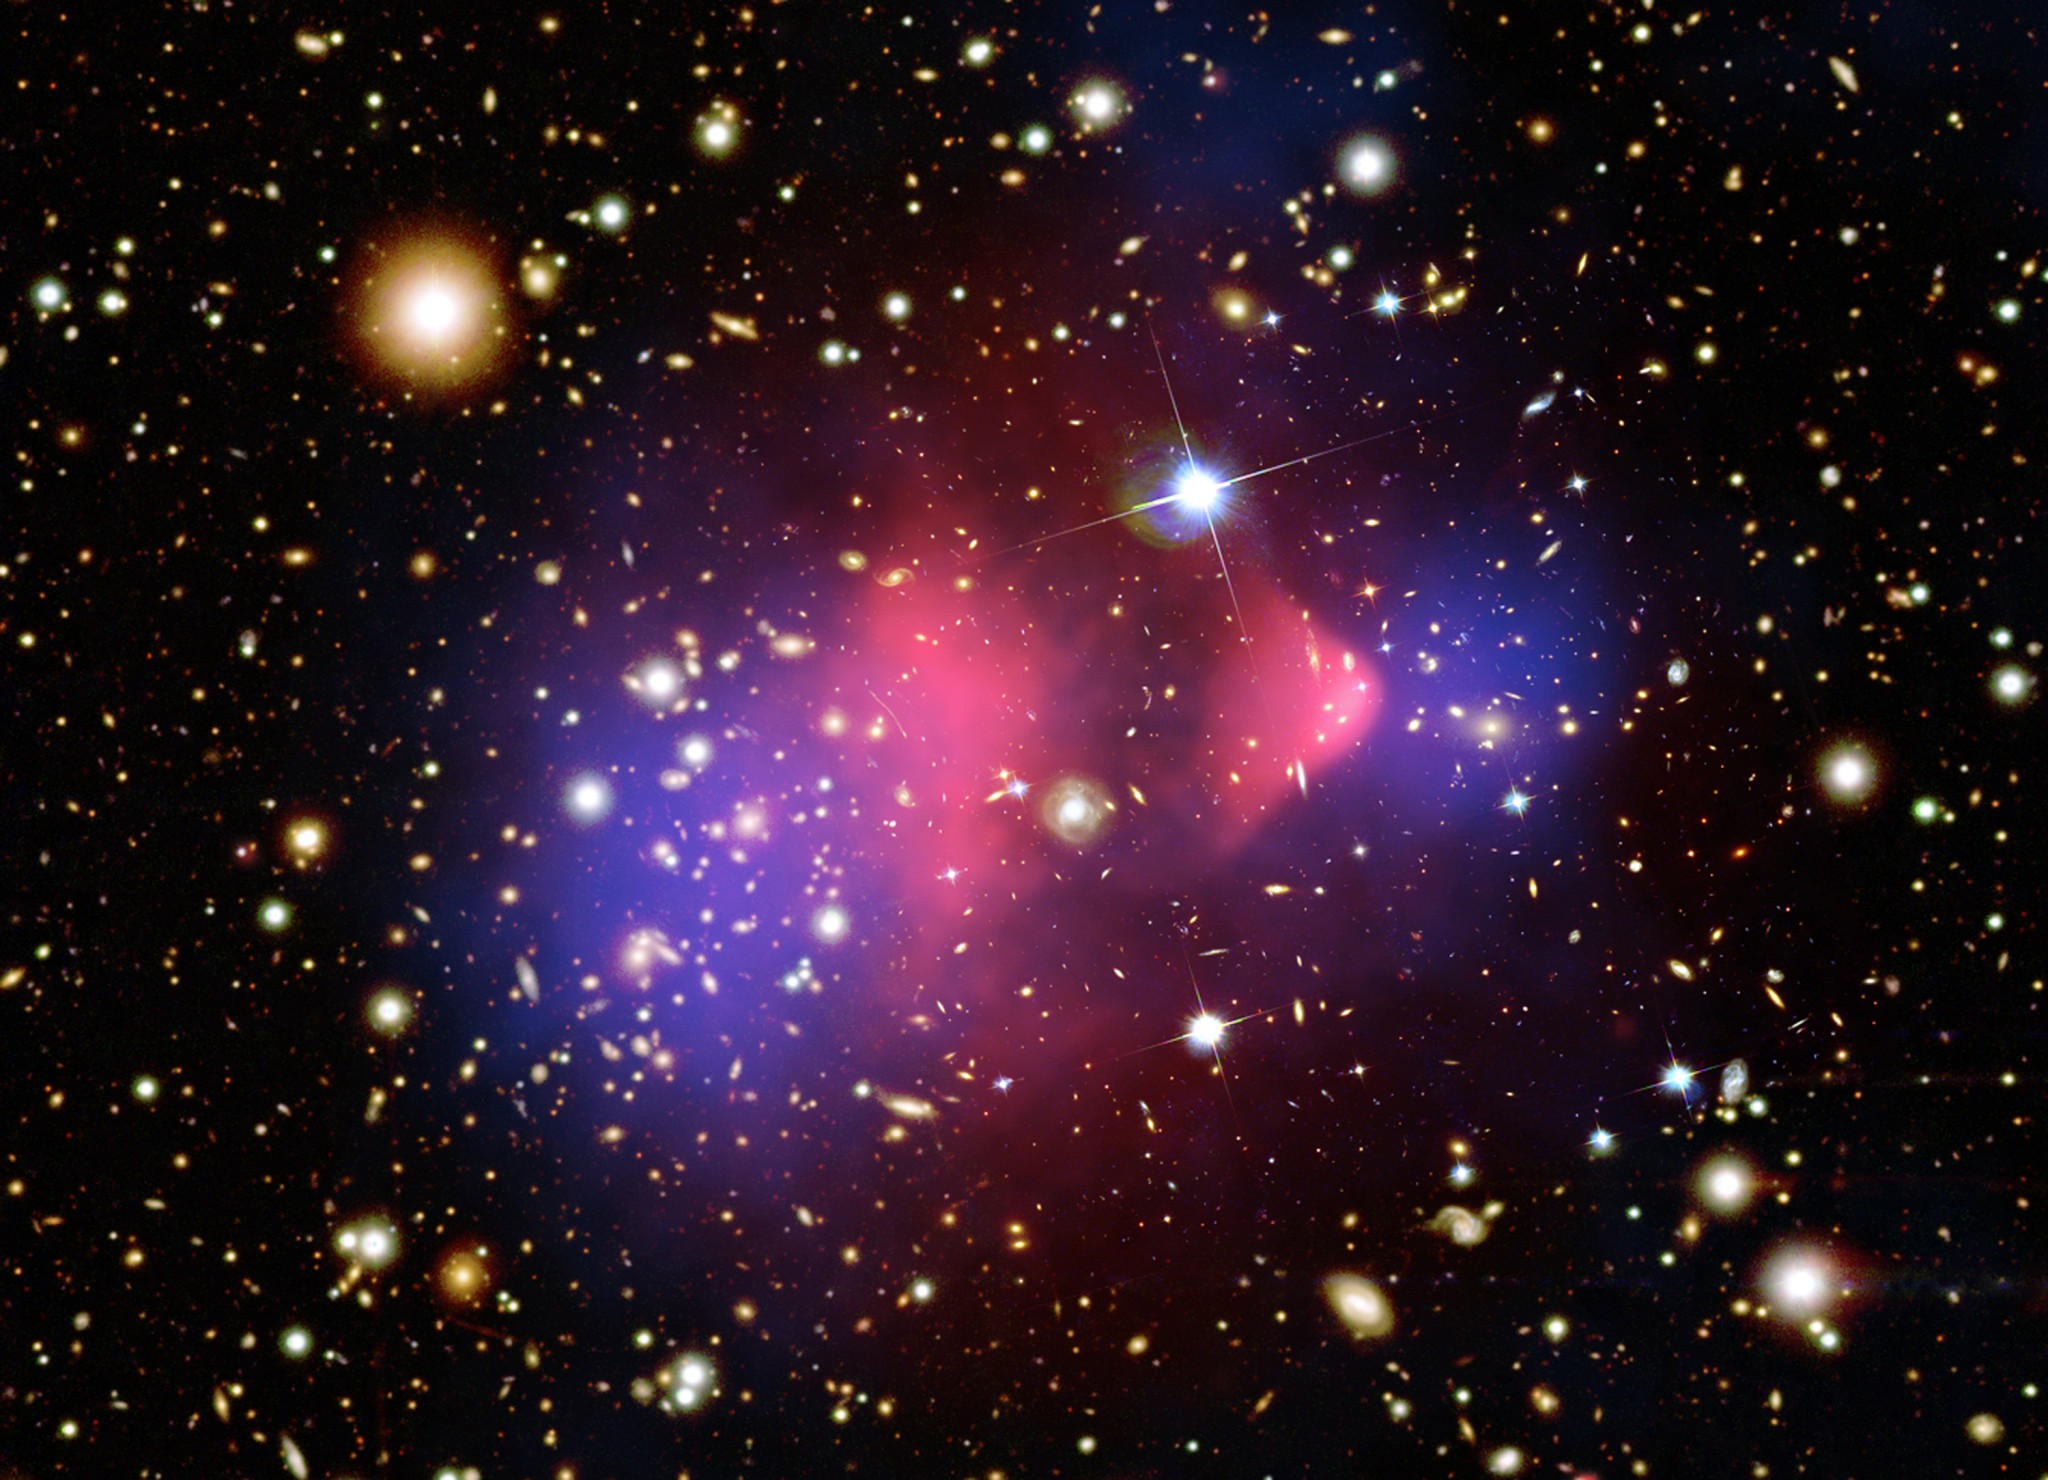
\includegraphics[height=5.5cm]{bulletcluster_comp_f2048.jpg}~%
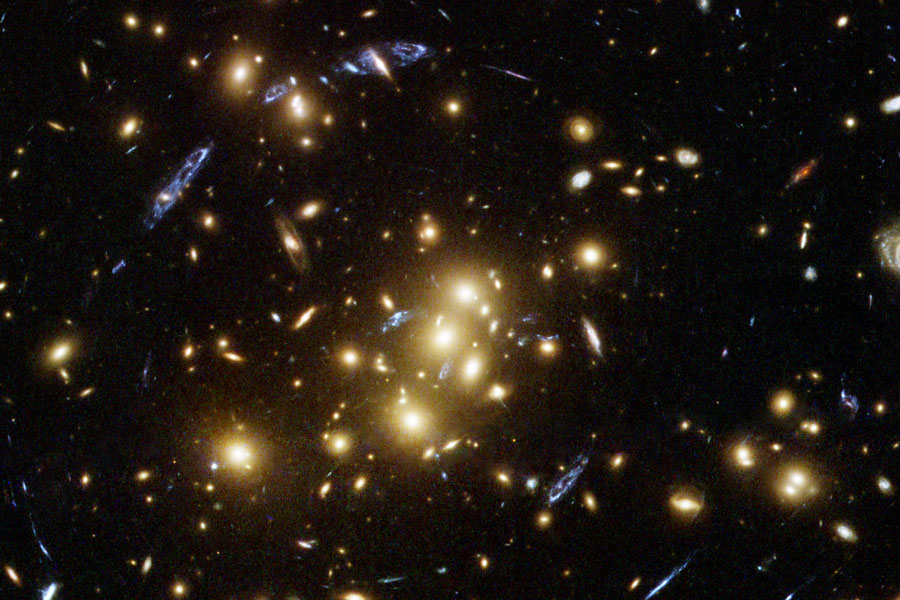
\includegraphics[height=5.5cm]{lentille-gravitationnelle.jpg}
\caption{\textbf{Left:} Composite optical image of the Bullet cluster, with X-ray in pink and weak gravitational lensing in blue (credit: NASA / STScI; ESO WFI; Magellan / U. of Arizona). \textbf{Right:} Gravitational lensing manifest near the 0024+1654 cluster (credit: HST), distorting the light rays from a background galaxy, shown as the stretched blue streaks.}
\label{fig:bullet}
\end{center}
\end{figure}

Despite the identity of a DM candidate particle still being speculative, it is nevertheless one of the most preponderant components of the Universe's energy density, second only to dark energy. As such, the current benchmark cosmological model is often refered to as the hot big bang $\Lambda$CDM model, where CDM stands for Cold Dark Matter. The ``cold'' adjective pertains to it having a narrow (quasi-Dirac) velocity distribution. In Sec.~\ref{sec:CAMB} in the next chapter, I distinguish cold dark matter from several non-cold dark matter cosmologies, the reason being that neutrinos --- the only DM candidate particle we've discovered --- cannot be cold as its velocity dispersion is to wide. This has a drastic impact on the formation of large scale structures and the distribution of the intergalactic gas, which I detail throughout this thesis.

\clearpage

\subsection*{Summary}

In an expanding Universe from a Hot Big Bang scenario described by a flat $\Lambda$CDM model, the expansion rate is driven by the energy density of a cosmological fluid through the Friedmann equations, which consists of three main components (radiation, matter and $\Lambda$) each having the following equations of state:\\

\begin{table}[!htbp]
	\begin{center}
		\begin{tabular}{cccc}
			\textbf{Component} & \textbf{Radiation} & \textbf{Matter} & \textbf{Dark Energy}\\[2pt]
			\hline \\[-10pt]
			Equation of State & $w_r = \cfrac{1}{3}$ & $w_m = 0$ & $w_\Lambda = -1$ \\[2pt]
			\hline \\[-10pt]
			Energy Density & $\rho_r \propto a^{-4}$ & $\rho_m \propto a^{-3}$ & $\rho_\Lambda \propto a^{0}$ \\[2pt]
			\hline \\[-10pt]
			Scale Factor & $a(t) \propto t^{1/2}$ & $a(t) \propto t^{2/3}$ & $a(t) \propto e^{H_0 \Omega_\Lambda^{1/2} t}$ \\[2pt]
			 & $a(\tau) \propto \tau$ & $a(\tau) \propto \tau^{2}$ & $a(\tau) \propto - 1/\tau$ \\[2pt]
			\hline \\[-10pt]
		\end{tabular}
	\end{center}
	%\label{tab:RDE_MDE}
\end{table}

In units of the critical energy density, the first Friedmann equation can be written: \\

\begin{equation}
\left( \frac{H(t)}{H_0} \right)^2 = \Omega^0_m a^{-3}(t) + \Omega^0_r a^{-4}(t) + \Omega^0_\Lambda
\end{equation} \\ This expression explicits the time dependance of the scale factor. Because the energy densities of these three components evolve distinctly with the scale factor, one can identify three epochs in the history of the Universe during which the radiation, matter and $\Lambda$ component dominates the others chronologically. One can determine when these epochs of domination swith from mainly radiation to mainly matter and finally to mainly $\Lambda$ (``matter - radiation equality'' and ``matter - $\Lambda$ equality'') by simply equating\\

\begin{align*}
\Omega_r (t) ~ a(t)^4 &= \Omega_r^0 ~ a_0^4\\
\Omega_m (t) ~ a(t)^3 &= \Omega_m^0 ~ a_0^3\\
\Omega_\Lambda (t) &= \Omega_\Lambda^0
\end{align*}\\

With today's values in Eqs.~\ref{eq:omega_lambda}, \ref{eq:omega_radiation} and \ref{eq:omega_matter}, one can straightforwardly compute that the cosmological constant dominates the dynamics of the observable Universe from $z=0$ to $z_\Lambda \simeq 0.3$. Prior to this redshift, the Universe was dominated by non-relativistic matter (matter dominated era or MDE) up to $z_{\mathrm{eq}} \simeq 3400$, prior to which was the radiation dominated era or RDE. Fig.~\ref{fig:cosmichistory} shows the evolution of $\Omega_r$, $\Omega_m$ and $\Omega_\Lambda$ with proper time, as well as that of the scale factor, and materializes the two equalities distinguishing the RDE from the MDE and the $\Lambda$DE. 

\begin{figure}
\begin{center}
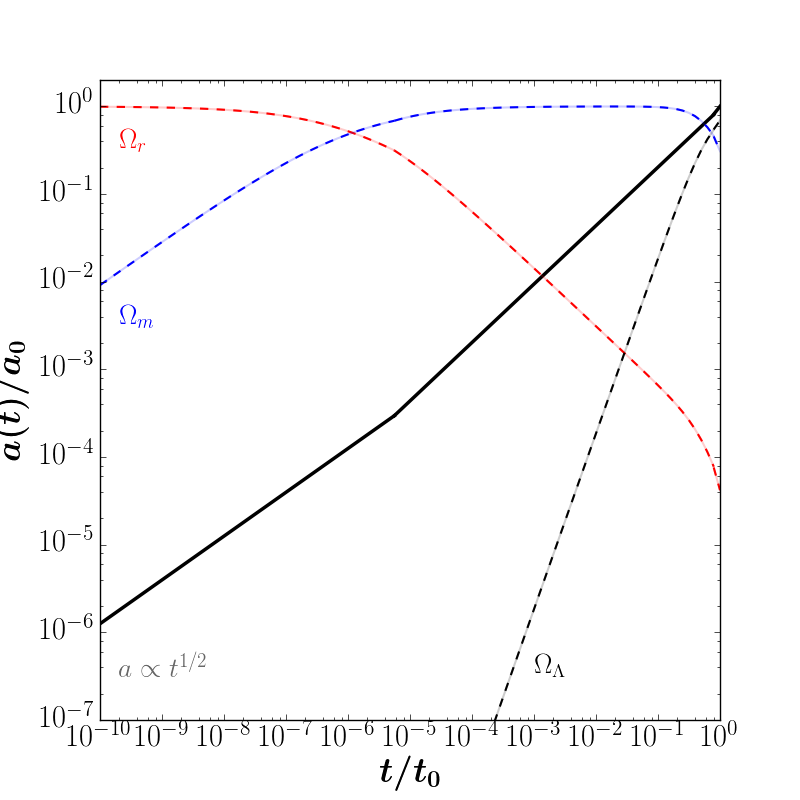
\includegraphics[width=0.75\columnwidth]{Cosmology/aa0.png}
\caption{Evolution of the radiation, matter and $\Lambda$ densities in units of critical density with respect to proper time (dot dashed color curves). The evolution of the scale factor in units of today's $a_0$ with proper time is superimposed as the solid black curve.}
\label{fig:cosmichistory}
\end{center}
\end{figure}

\clearpage



\setcounter{chapter}{2}
\chapter{A Structured Universe}
{\color{purple}\titlerule[2.5pt]}
\vspace{4pc}%
\label{chap:structure}
%\tikz[remember picture,overlay] \node[opacity=0.3,inner sep=0pt] at (current page.center){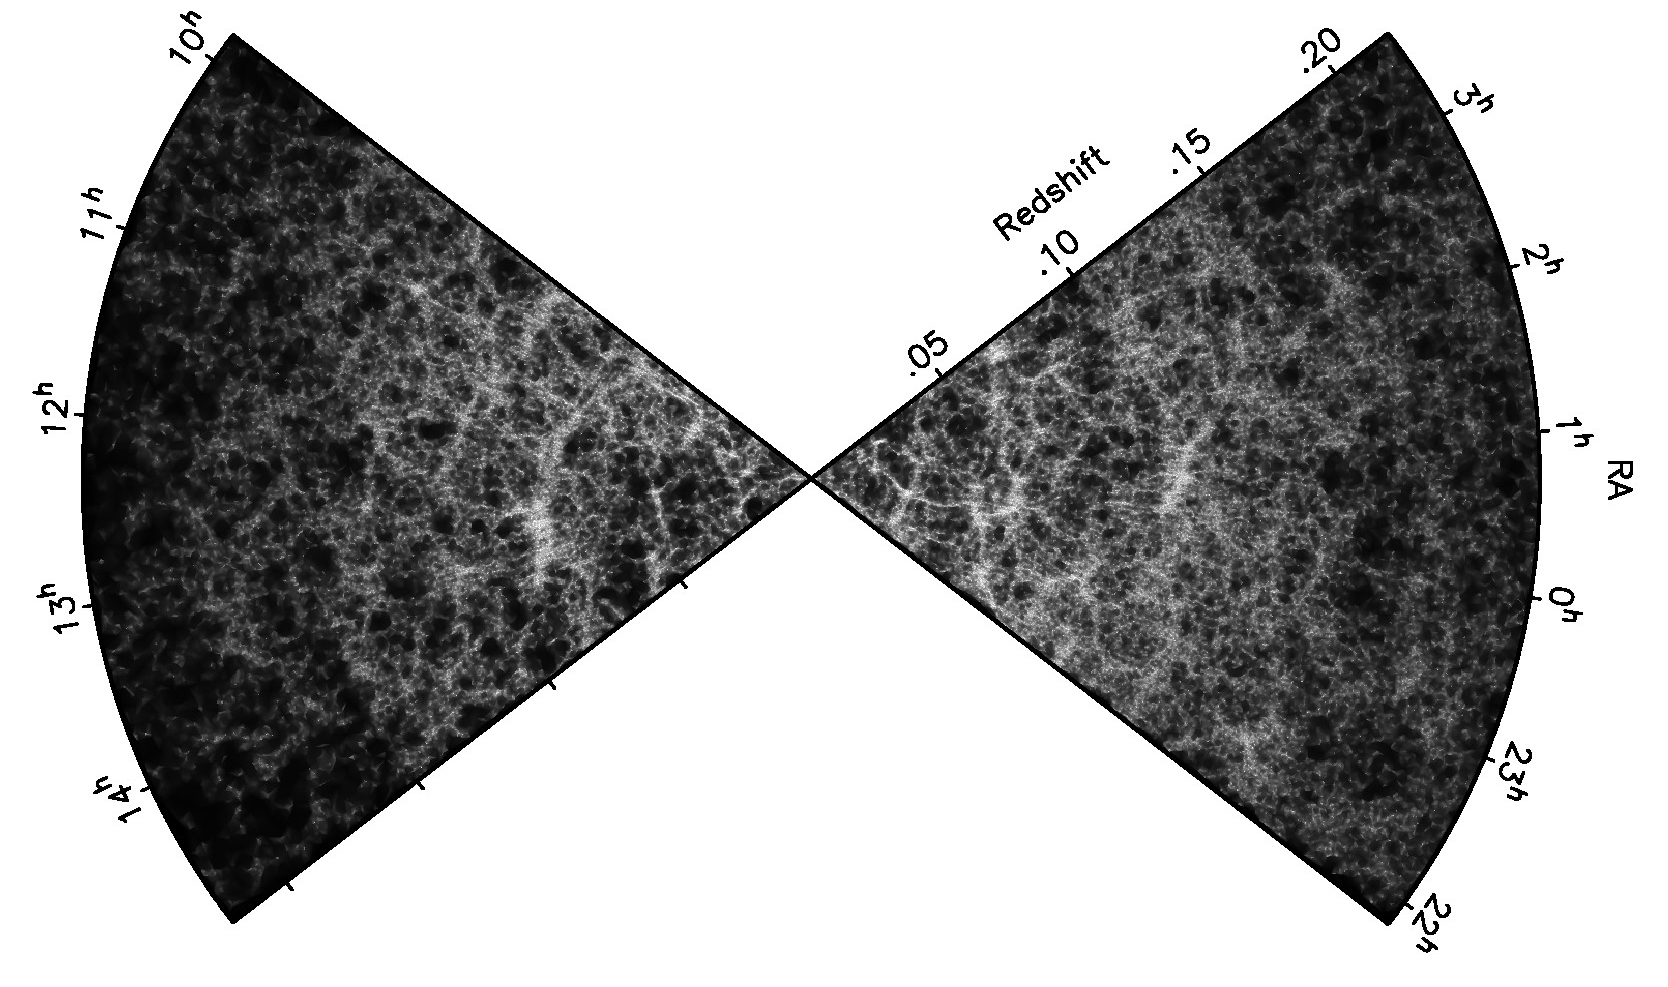
\includegraphics[height=0.8\paperwidth, angle=-90, keepaspectratio]{2dfgrs.png}};
{\centering
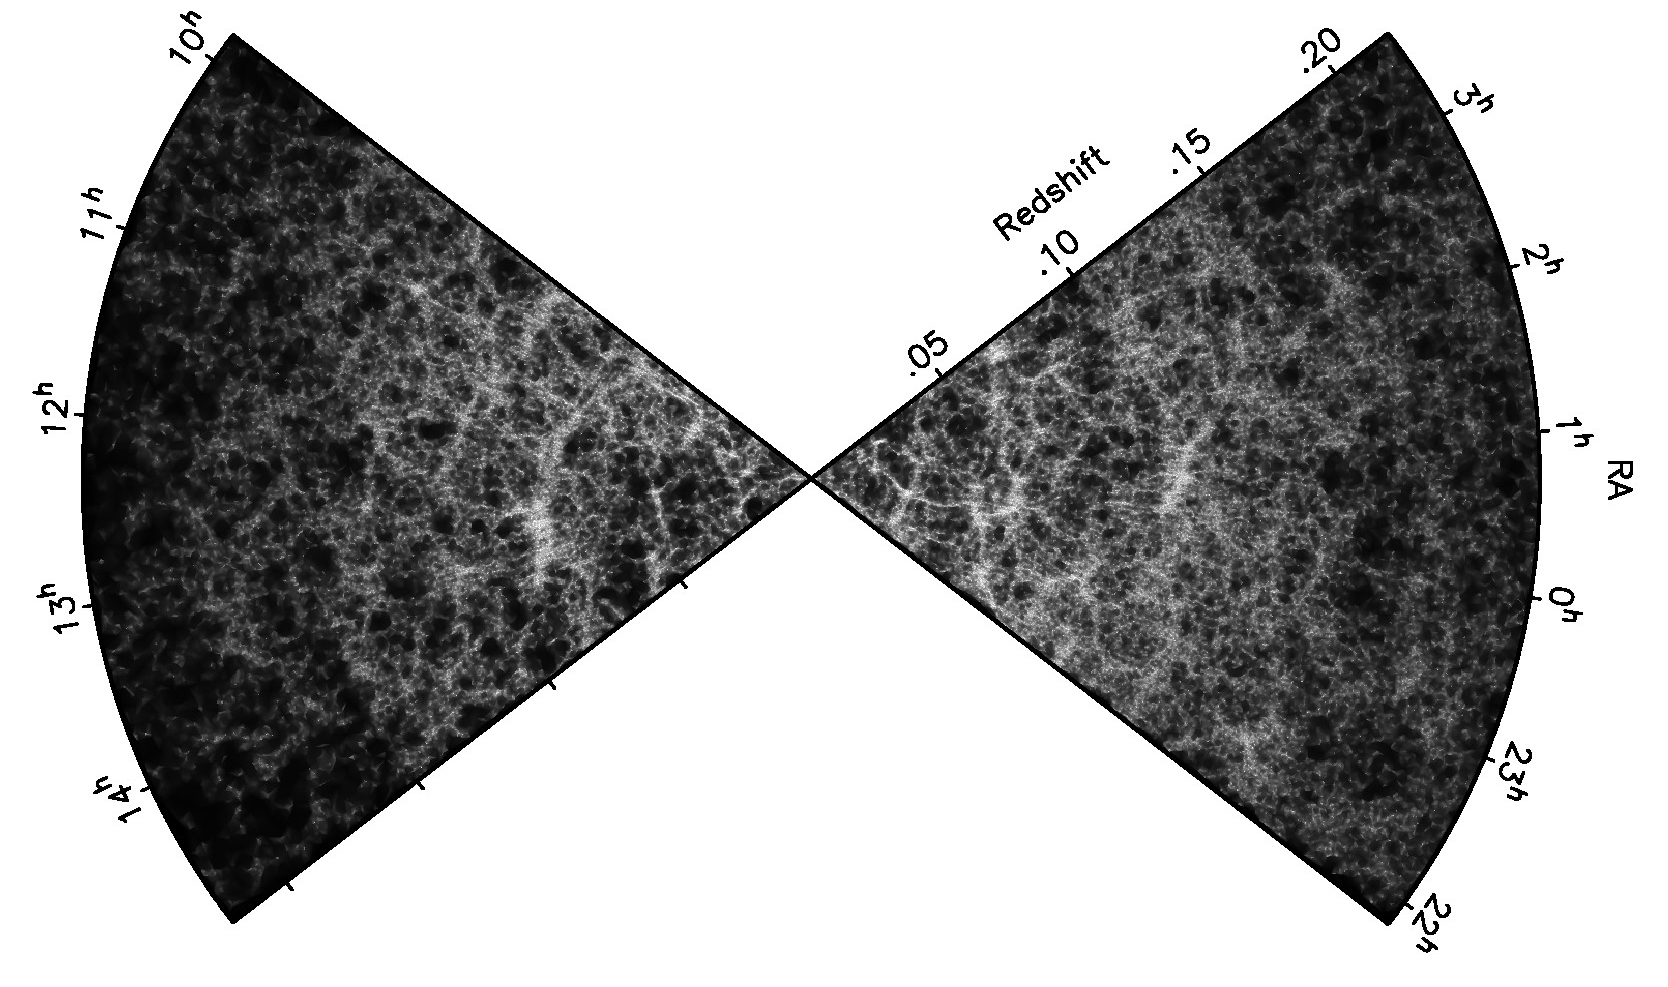
\includegraphics[width=\textwidth]{2dfgrs.png}}
\clearpage

	\vspace*{3pc}
\begin{center}
\begin{minipage}{0.7\linewidth}
\hrule
\vspace{8pt}
{\huge\guillemotleft} ~The light shines in the darkness, and the darkness has not overcome it. {\huge\guillemotright}  \\
\vspace{2pt}
\begin{flushright}
--- \textsc{John 1:5}
\end{flushright}
\vspace{8pt}
\hrule
\end{minipage}
\end{center}
\vspace{3pc}

%\section*{Introduction}
\begin{intro}
{\color{purple}I}n the previous chapter, I detailed the impact of neutrino mass on the matter power spectrum. This was under the assumption that one can linearly perturb the density fields around their background value. However, since $\delta$ increases monotonically due to the attractive nature of the gravitational interaction, the approximation of linear theory eventually breaks down below some scale $k_0$. Linear theory remains valid as a perturbative treatment for $k < k_0$ where \\
\end{intro} 
\begin{equation*}
\begin{array}{c}
k_0^3 ~\vert \delta(k_0) \vert^2 \sim 1 \\
\Leftrightarrow \\
\Delta^2 (k_0) \sim 1 \\
\Leftrightarrow \\
\sigma^2 (1/k_0) \sim 1
\end{array}
\end{equation*} \\ For higher $k$ values, the evolution of $\delta$ is said to be \emph{non-linear}. One must explicitely solve the gravitational interactions between particles with numerical simulations. This is layed out in the following chapter. In the present chapter, I lay out how the power spectrum can be measured in the non-linear regime. In Sec.~\ref{sec:p1d}, I introduce quasi-stellar objects, which are the brightest sources of light in the Universe. The spectrometric properties of their light observed with Earth telescopes give us valuable information on their environment through their atomic spectral emission lines. The absorption lines, on the other hand, yield information on the intergalactic medium in which their light travels. A particular region of interest is the region blueward of the Lyman-alpha emission line, which entails the redshift and density of Hydrogen absorbers along the quasar line-of-sight. Known as the Lyman-alpha forest, it is a very active area of research for both extragalactic astrophysicists and cosmologists. I also introduce the main observable for this work: the power spectrum of the transmitted flux fraction in the Lyman-$\alpha$ forest of quasars. In Sec.~\ref{sec:pfdata}, I describe three sets of quasar samples taken from large scale structure surveys, from which I compute the Lyman-alpha power spectrum. 

	
	\section{Probing Inhomogeneities ~\&~ Anisotropies}
	\label{sec:PS}
	\vspace*{1.5pc}

It is expected that spatial homogeneity and isotropy break down on some scale. However, it is empirically verified that the Universe is \emph{statistically} homogeneous and isotropic. Take a look at the distribution of galaxies on the background figure on page~\pageref{chap:structure} for instance. At first glance, the cosmological principle holds: the distribution of large scale structures appears to be the same in whatever direction from the center you look in. In terms of spatial averages, the background distribution is in practical terms homogenous. But average out the distribution in smaller and smaller patches anywhere on the map and you may start to notice some dissimilarities from one patch to another of same dimensions. On really small scales, the distribution could hardly be more heterogenous: in some tiny patches, you may end up with a bunch of clumps or clusters of galaxies while in other barely if any. The characterisation of these inhomogeneities as one averages out over shorter and shorter volumes is grounded in a mathematical concept called the \textbf{power spectrum}. The wider the patch on which we average, the less of them we can place in our total available volume. This sampling variance --- or cosmic variance --- makes our statements about the largest of scales statistically less robust than on smaller scales since we cannot compare the entire observable Universe to anything else ! This won't limit our appreciation of the power spectrum as a powerful tool to probe large scales structures however, since we've already settled the global background evolution.

%%%%%%%%%%%%%%%%%%%%%%%%%%%%%%%%%%%%%%%%%%%%%%%%%%%%%
\subsection{Power Spectra: Definition}
%%%%%%%%%%%%%%%%%%%%%%%%%%%%%%%%%%%%%%%%%%%%%%%%%%%%%

\subsubsection{Inhomogeneities}

To study inhomogeneities in a generic density field $\varepsilon (\vec{x}, t)$, we can expand it to a mean value $\bar{\varepsilon} (t) = \langle \varepsilon(\vec{x},t) \rangle$ averaged over a hypersurface of simulatenity at time $t$ and a density contrast $\delta_\varepsilon$ in the field, large or small:
\begin{equation}
\label{eq:field}
\varepsilon(\vec{x}, t) = \bar{\varepsilon} (t) \left( ~1 ~+~ \delta_\varepsilon (\vec{x}, t) ~ \right)
\end{equation}
In the framework of cosmology, we will use conformal time $\tau = a^{-1} t$ instead of proper time and work in Fourier space\footnote{this is useful because each mode can be treated as evolving independantly of one another}, in which $\vec{\nabla}_{\vec{x}} \rightarrow - i \vec{k}$ and
\begin{equation}
\label{def:fourier}
\tilde{\varepsilon} (\vec{k}, \tau) = \mathcal{F}\left[ \varepsilon (\vec{x}, \tau) \right] = \int \frac{d^3 x}{(2 \pi)^3}~ \varepsilon(\vec{x}, \tau) e^{-i \vec{k} \cdot \vec{x}}
\end{equation}\\
It is clear from Eq.~\ref{eq:field} that the mean value of the field makes the average of the contrast null when averaged over a large enough volume. Making the time dependance implicit, we may characterize the variance in the field, by introducing
\begin{equation}
\label{def:ps_generic}
\left\{
\begin{array}{l}
\langle \delta_\varepsilon (\vec{k}) \rangle = 0\\
\\
\langle \delta_\varepsilon (\vec{k}) \delta_\varepsilon (\vec{k}^\prime) \rangle \doteq (2 \pi)^3~\delta^{\mathrm{(D)}} (\vec{k} - \vec{k}^\prime) \times P_\varepsilon (\vec{k})
\end{array}
\right.
\end{equation} where the Dirac distribution is defined as
\begin{equation}
\label{df:dirac_distrib}
\delta^{\mathrm{(D)}} (\vec{x}) = \left\{
\begin{array}{ll}
1 & \text{at}~ \vec{x} = \vec{0}\\
0 & \text{elsewhere}
\end{array}
\right.
\end{equation} $P_\varepsilon$ is known as the auto-correlation power spectrum of field $\varepsilon$, to distinguish it from the cross-correlation power spectrum of fields $\varepsilon$ and $\eta$, which is defined as
\begin{equation}
\langle \delta_\varepsilon (\vec{k}) \delta_\eta (\vec{k}^\prime) \rangle \doteq (2 \pi)^3~\delta^{\mathrm{(D)}} (\vec{k} - \vec{k}^\prime) \times P_{\varepsilon \eta} (\vec{k})
\end{equation}  It quantifies the contribution of each $\vec{k}$ vector mode to the field's variance and has the dimensions of a volume since $\vec{k}$ is the canonical conjugate of a spatial vector. When one considers a finite volume $\mathbb{V}$ with periodic conditions, the power spectrum can be interpreted as 
\begin{equation}
P_\varepsilon (\vec{k}) = \lim_{\mathbb{V} \rightarrow \infty} \frac{\langle \vert \delta_\varepsilon (\vec{k}) \vert^2 \rangle}{\mathbb{V}}
\end{equation} Assuming isotropy, the power spectrum does not depend on the direction $\hat{k} = \vec{k}/k$ but only on its magnitude $k = \vert \vec{k} \vert$: $P_\varepsilon (\vec{k}) = P_\varepsilon(k)$\\

\subsubsection{Anisotropies}

I will also consider fields which only depend on the relative orientation of momentum $\vec{p} = p \hat{p}$ with mode $\vec{k} = k \hat{k}$. Noting $\mu = \hat{p} \cdot \hat{k}$ the cosine of their relative angle, the relative fluctuation or contrast in field $\theta_X = \delta X / \bar{X}$ can be expanded into spherical harmonics
\begin{equation}
\label{eq:field_tensor}
\theta_X (\hat{k}, \mu) = \sum_{\ell = 1}^{\infty} \sum_{m = - \ell}^{+\ell} a^X_{\ell m} (\hat{k}, \mu) \mathcal{Y}_{\ell m} (\hat{p})
\end{equation} where
\begin{equation}
a^X_{\ell m} (\hat{k}, \mu) = (-i)^\ell 4\pi ~\iint d\Omega ~ \mathcal{Y}^{\ast}_{\ell m} (\hat{p}) \tilde{\theta}_X (\hat{k}, \mu)
\end{equation} and
\begin{equation}
\iint d\Omega ~\mathcal{Y}_{\ell m} (\hat{p}) \mathcal{Y}^{\ast}_{\ell^\prime m^\prime} (\hat{p}) = \delta_{\ell \ell^\prime} \delta_{mm^\prime}
\end{equation} The mean value being zero, the variance again defines a power spectrum. Here, the cross-correlation between $X$ and $Y$:
\begin{equation}
\label{eq:ps_ang_corr}
\left\{
\begin{array}{lcl}
\langle a^X_{\ell m} \rangle & = & 0\\
\\
\langle a^X_{\ell m} a^{Y,\ast}_{\ell^\prime m^\prime} \rangle  & = & \delta_{\ell \ell^\prime} \delta_{mm^\prime} \mathcal{C}^{XY}_\ell
\end{array}
\right.
\end{equation} where $\mathcal{C}_\ell$ has no dependance on $m$ because of  isotropy. $X$ and $Y$ can be scalar modes (\textit{e.g.} temperature) or tensor modes (\textit{e.g.} polarizations $+$ and $\times$, or $E$ and $B$). 



%%%%%%%%%%%%%%%%%%%%%%%%%%%%%%%%%%
\subsection{Matter Power Spectrum}
%%%%%%%%%%%%%%%%%%%%%%%%%%%%%%%%%%

\begin{figure}[!]
\begin{center}
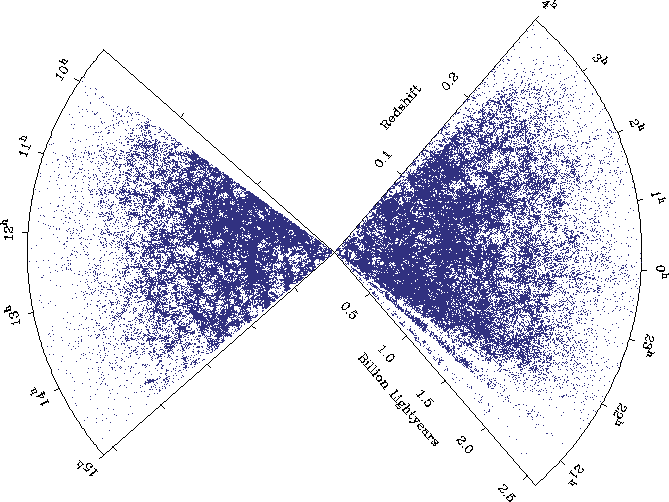
\includegraphics[height=5.5cm]{galaxies_2dFGRS_big.png}~%
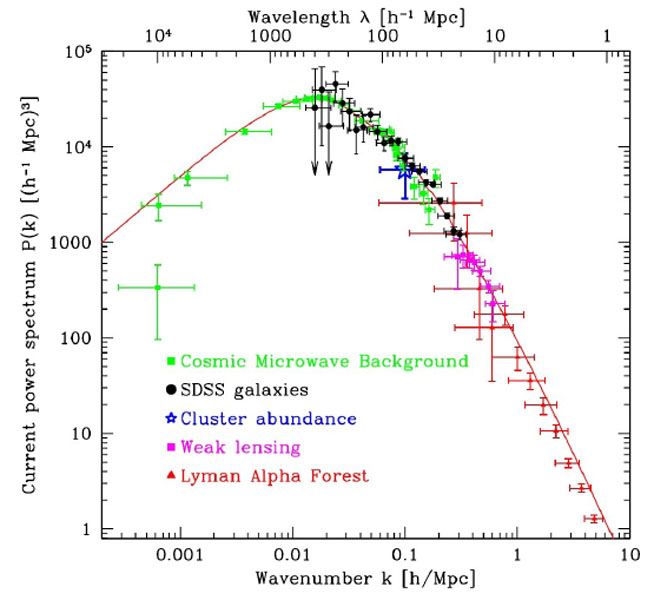
\includegraphics[height=5.5cm]{PS_z0.jpg}
\caption{\textbf{Left:} Distribution of galaxies within $2.5 \times 10^9$ light years of the Milky Way (center). Credit: 2dF Galaxy Redshift Survey. \textbf{Right:} Matter power spectrum measured at $z=0$ using 5 probes. The solid line is the best fitted $\Lambda$CDM model. Credit: \cite{PowerSpectrum_Tegmark}}
\label{fig:LSS}
\end{center}
\end{figure}

\subsubsection{Inhomogeneities in the Matter Distribution}

As I will detail in the next section, the density field of non-relativistic matter is only sensitive to monopolar perturbations, and so we may define the power spectrum of matter density contrast  at redshift $z$ as \\
\begin{empheq}[box=\mymath]{equation}
P_m (k, z) = \langle \vert \delta_m (k, z) \vert^2 \rangle
\end{empheq} \\ where
\begin{equation}
\delta_m (k, z )= \frac{\sum\limits_{i \in \lbrace cdm, b, \nu \rbrace} \bar{\rho}_i (z) \delta_i (k, z)}{\sum\limits_{i \in \lbrace cdm, b, \nu \rbrace} \bar{\rho}_i (z)}
\end{equation} when neutrinos are massive. The left-hand side of Eq.~\ref{def:ps_generic} for $\varepsilon = m$ is the auto-correlation function of non-relativistic matter. Since dark matter cannot be detected via electromagnetic waves, we can only infer its presence indirectly, using its impact on \emph{tracers}, \textit{i.e.} massive objects, commonly galaxies and quasars. It is clear from Eq.~\ref{def:ps_generic} that the power spectrum of these tracers and their correlation function $\xi(r)$ are a Fourier Transform pair
\begin{equation}
\xi (r) = \int \frac{d^3 k}{(2 \pi)^3} ~P(k)~ e^{i \vec{k} \cdot \vec{r}}
\end{equation} Because of isotropy, the correlation function is symmetric under rotation meaning it is only function of the relative position of objects $\xi(\vec{r}) = \xi(r)$, or equivalently $P(\vec{k}) = P(k)$. 
The power spectrum of these biased tracers can be linked to that of the underlying matter distribution by a real number $b \in \mathbb{R}$
\begin{equation}
P_{\mathrm{tracer}}(k) = b^2_{\mathrm{tracer}} P_m (k)
\end{equation} which is specific to the tracer used. When measuring the power spectrum of such a tracer, one must also take into account redshift distortion due to the peculiar velocity of the tracer which adds a Doppler shift (either blue-ward or red-ward) which skews the redshift along the line-of-sight. This anisotropy induced in the power spectrum is characterized by the Kaiser $\beta$ parameter \citep{Kaiser1987}:
\begin{equation}
P(k, \mu) = (1 + \beta ~\mu^2 k)^2 P(k)
\end{equation}\\

Finally, for objects on which we can only probe a density field along a line-of-sight such as for Lyman-alpha forests (see Sec.~\ref{sec:p1d}), it is useful to use the unidimensional power spectrum $P_{\mathrm{1d}}$ which is linked to the three-dimensional one by
\begin{empheq}[box=\mymath]{equation}
\label{eq:1dpwrspctrm}
\begin{array}{cl}
P_{\mathrm{1d}} (k_{\parallel}) &= \displaystyle \int \cfrac{d \vec{k}_{\bot}}{(2 \pi)^2}~ P_{\mathrm{3d}}(\vec{k}) \\
 &= \displaystyle \int \cfrac{dk}{2 \pi}~k P(k)
\end{array}
\end{empheq} where the mode vector $\vec{k} = (k_{\parallel}, \vec{k}_{\bot})$ is decomposed into a divergence-free (scalar) and a curl-free (vector) components. When not explicitely specified, $P(k) = P_{\mathrm{3d}}(k)$.\\


%It is helpful in computing the variance of $\delta$, since
%\begin{equation}
%\label{eq:variance_ps}
%\langle \delta^2 (\vec{r}) \rangle = \int_0^\infty \frac{dk}{k} \Delta^2 (k)
%\end{equation}
A very useful quantity to grasp the physical meaning of the power spectrum is the variance per logarithmic $k$, \textit{a.k.a.} the dimensionless power spectrum, defined as \\
\begin{empheq}[box=\mymath]{equation}
\label{eq:variance_ps}
\Delta^2 (k) \doteq \frac{k^3 P(k)}{2 \pi^2}
\end{empheq} \\ It is linked to the one-point variance of the density field 
\begin{align*}
\xi (r=0) &= \langle ~ \delta^2(0) ~ \rangle \\
&= \int \frac{\mathrm{d}^3\vec{k}}{(2 \pi)^3} ~ P(\vec{k}) \\
&= \int \frac{\mathrm{d}k}{2 \pi^2} ~ k^2 P(k) \\
&= \int \mathrm{d}\ln k ~ \frac{k^3 P(k)}{2 \pi^2} \\
&= \int \mathrm{d}\ln k ~ \Delta^2 (k)
\end{align*} To have a finite variance, which we assume to always have in cosmology, we require:
\begin{eqnarray}
\Delta^2 (k) \longrightarrow \left\{ \begin{array}{ccl}
0 &\text{as}& k \rightarrow 0\\
0 &\text{as}& k \rightarrow \infty
\end{array}
\right.
\end{eqnarray} In other words, if the power spectrum is polynomial $P(k) \sim k^n$, then, 
\begin{eqnarray}
n ~\left\{ \begin{array}{ccl}
> -3 &\text{as}& k \rightarrow 0\\
< -3 &\text{as}& k \rightarrow \infty
\end{array}
\right.
\end{eqnarray} Note that the power spectrum can diverge as $k \rightarrow 0$.\\



\subsubsection{Link with Real-Space Fluctuations}

Let $m(\mathbb{V}) = \displaystyle \int_\mathbb{V} \mathrm{d}^3 \vec{r} ~\rho(\vec{r})$ be the mass in a finite volume $\mathbb{V}$. The normalized mass fluctuation in volume $\mathbb{V}$ is defined as
\begin{equation}
\sigma^2 (\mathbb{V}) \doteq \frac{( m(\mathbb{V}) - \langle m(\mathbb{V}) \rangle)^2}{\langle m(\mathbb{V}) \rangle^2}
\end{equation} By substituting the density contrast and the auto-correlation of its field, it is straightforward to show that
\begin{equation}
\sigma^2_\mathbb{V} = \int \mathrm{d}^3 \vec{k} ~P(\vec{k})~ \vert W_\mathbb{V} (\vec{k}) \vert^2
\end{equation} where
\begin{equation}
W_\mathbb{V} (\vec{k}) = \frac{1}{\mathbb{V}} \int_\mathbb{V} \mathrm{d}^3 \vec{r} ~e^{i \vec{k} \cdot \vec{r}}
\end{equation} is the Fourier Transform of the following window function
\begin{eqnarray}
W_\mathbb{V} (\vec{r}) = \left\{ \begin{array}{cl}
1/\mathbb{V} &\text{where}~ \vec{r} \in \mathbb{V}\\
0 &\text{everywhere else}
\end{array}
\right.
\end{eqnarray} \\ In the case where $\mathbb{V}$ is a sphere of radius $R$, 
\begin{equation}
W_\mathbb{V} (\vec{r}) = \frac{3}{4 \pi R^3} ~\mathcal{H}(R-r)
\end{equation} where $\mathcal{H}$ is the Heavyside function. Computing its Fourier Transform
$$ \tilde{W}_R (\vec{k}) = \frac{3}{(kR)^3} ~ \left( \sin kR ~- kR \cos kR \right) $$ and assuming a power spectrum of the form $P(k) \sim A k^n$, the normalized mass function in the sphere of radius $R$ takes the form $$ \sigma^2(R) = 9AR^{-(n+3)} \int_{0}^{kR} d^3 y ~ y^{n-6} \left( \sin y - y \cos y \right)^2 $$ For $n>1$ on one hand, $\sigma^2 (R) \propto R^{-4}$. For $n<1$ on the other hand, the above integral converges as $kR \rightarrow \infty$ and
\begin{align*}
\sigma^2(R) &\propto AR^{-(n+3)} \\
&\propto \Delta^2 (k = R^{-1}) \\
&\propto \left[ k^3 P(k) \right]_{k=R^{-1}}
\end{align*} \\
For what follow, we will denote the mass variance within a co-moving radius of $R=8 ~h^{-1}$Mpc as
\begin{empheq}[box=\mymath]{equation}
\label{def:sig8}
\sigma_8 \doteq \sqrt{\sigma^2(R=8~h^{-1}\mathrm{Mpc})}
\end{empheq}


\begin{figure}
\begin{center}
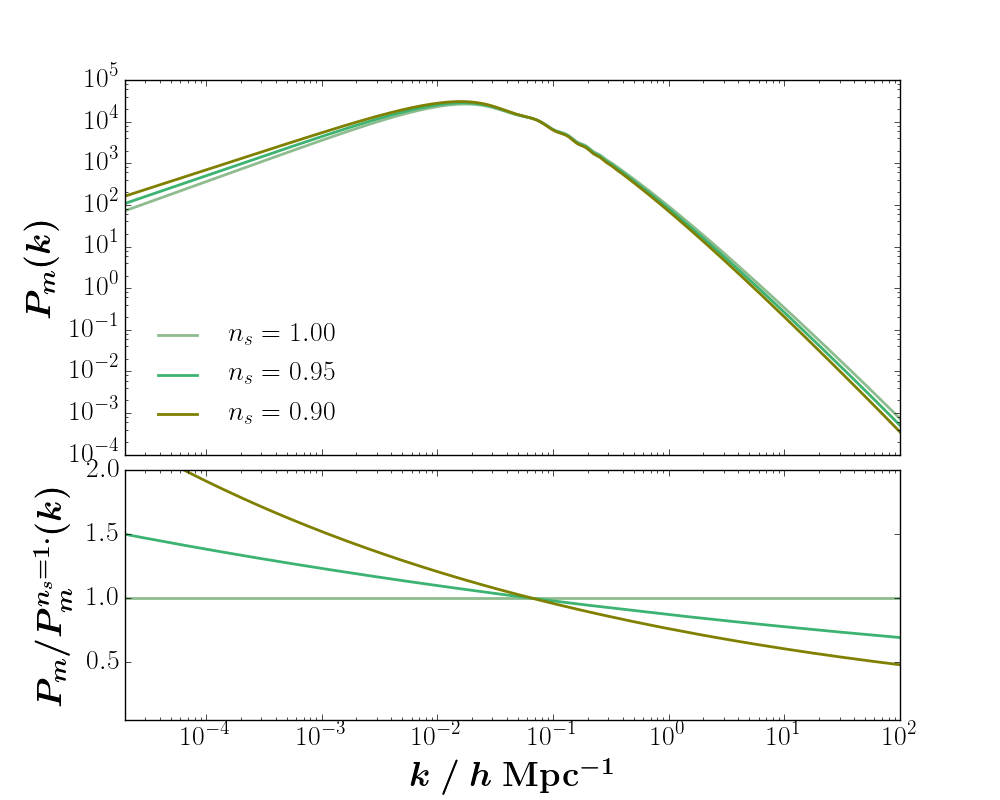
\includegraphics[width=0.65\linewidth]{CosmoParam/Pk_ns.png}
%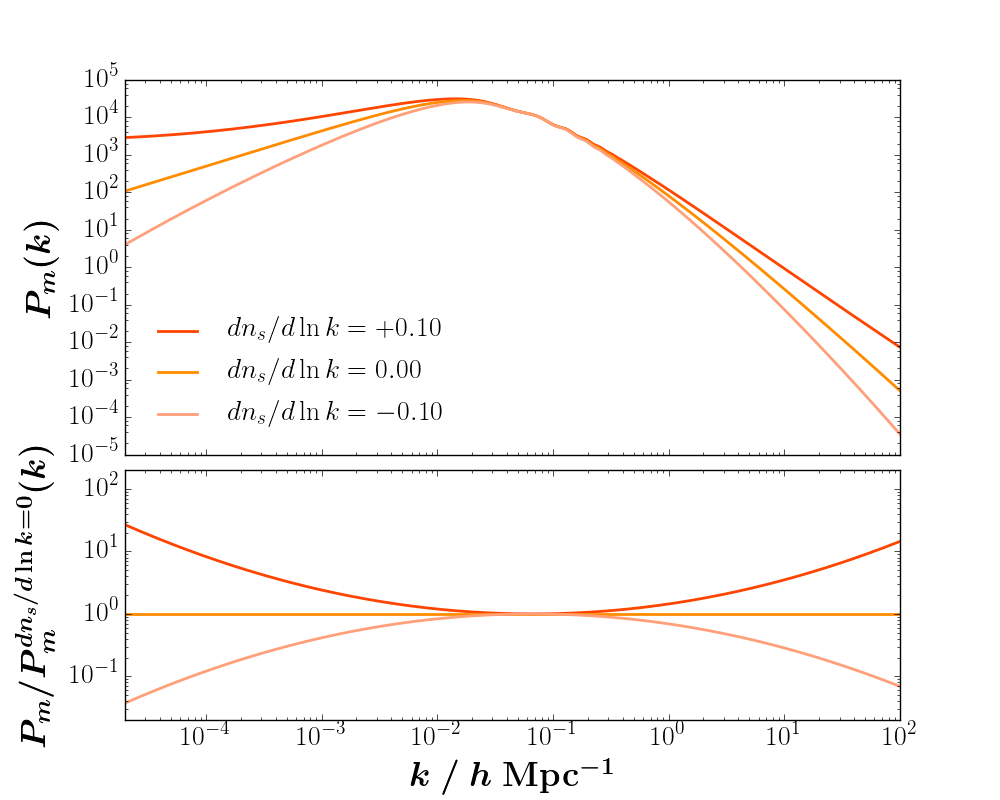
\includegraphics[width=0.4\linewidth]{CosmoParam/Pk_nrun.png}
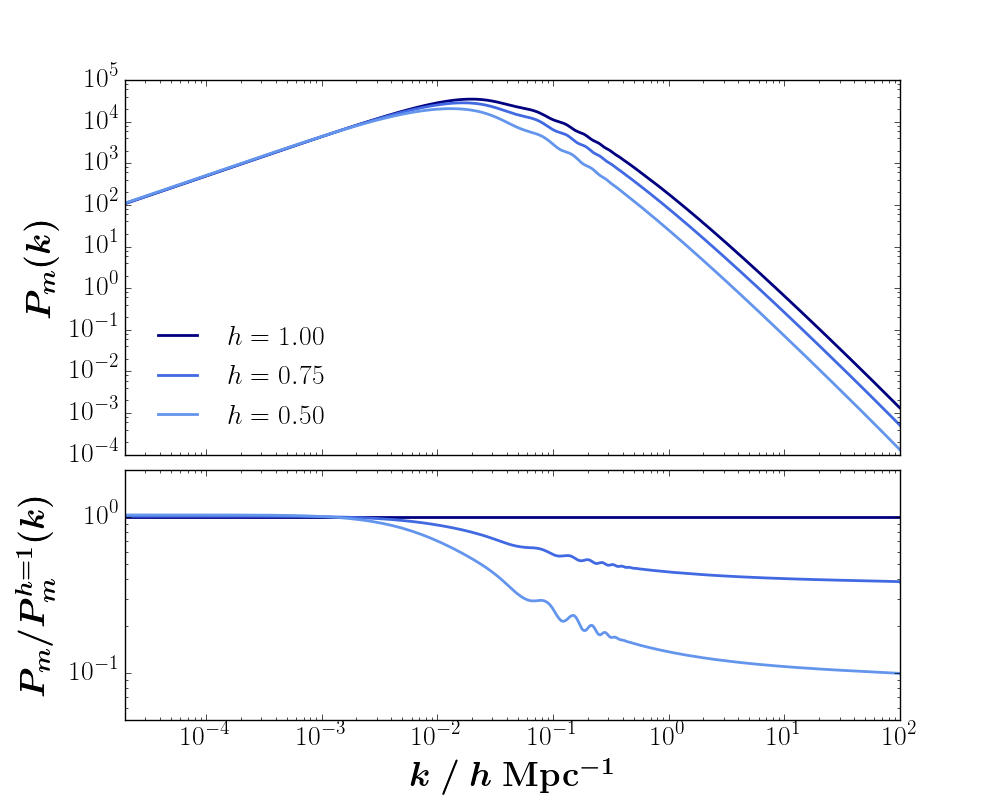
\includegraphics[width=0.65\linewidth]{CosmoParam/Pk_h.png}
%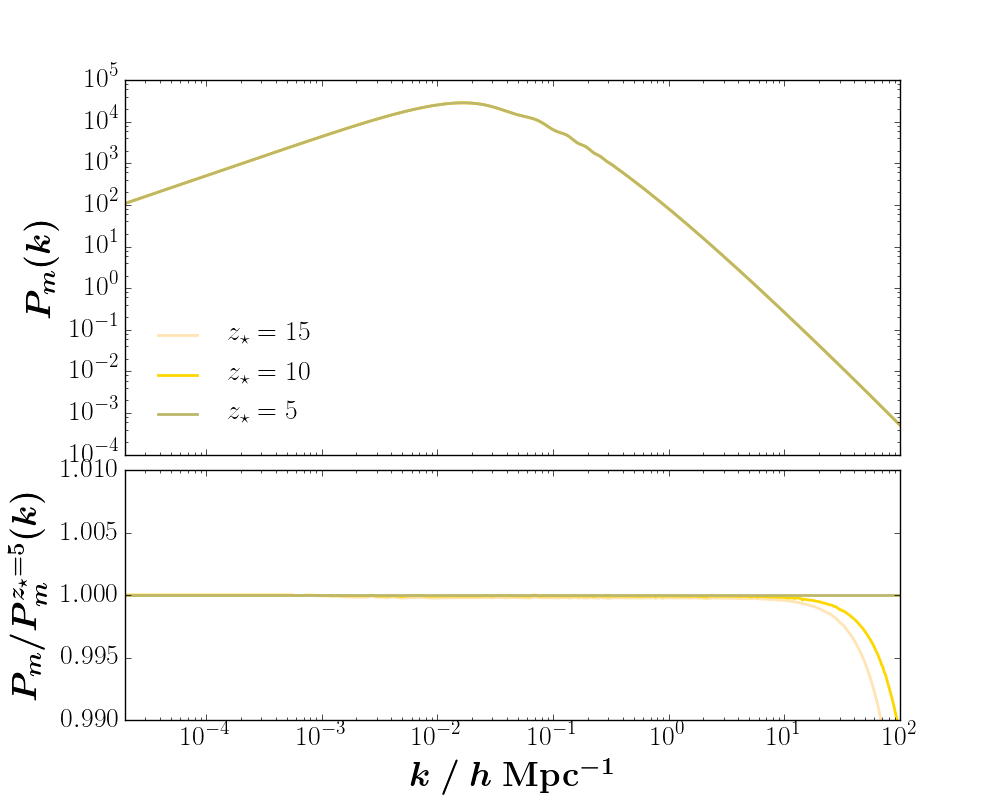
\includegraphics[width=0.4\linewidth]{CosmoParam/Pk_zreio.png}
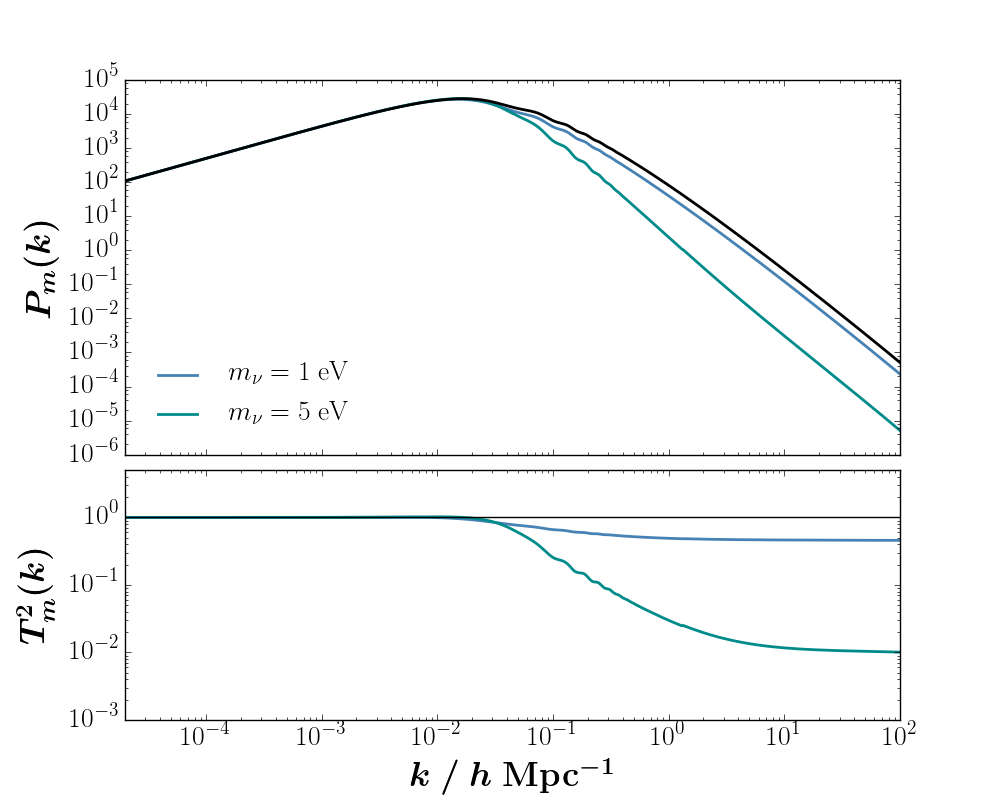
\includegraphics[width=0.65\linewidth]{CosmoParam/Pk_mnu.png}
%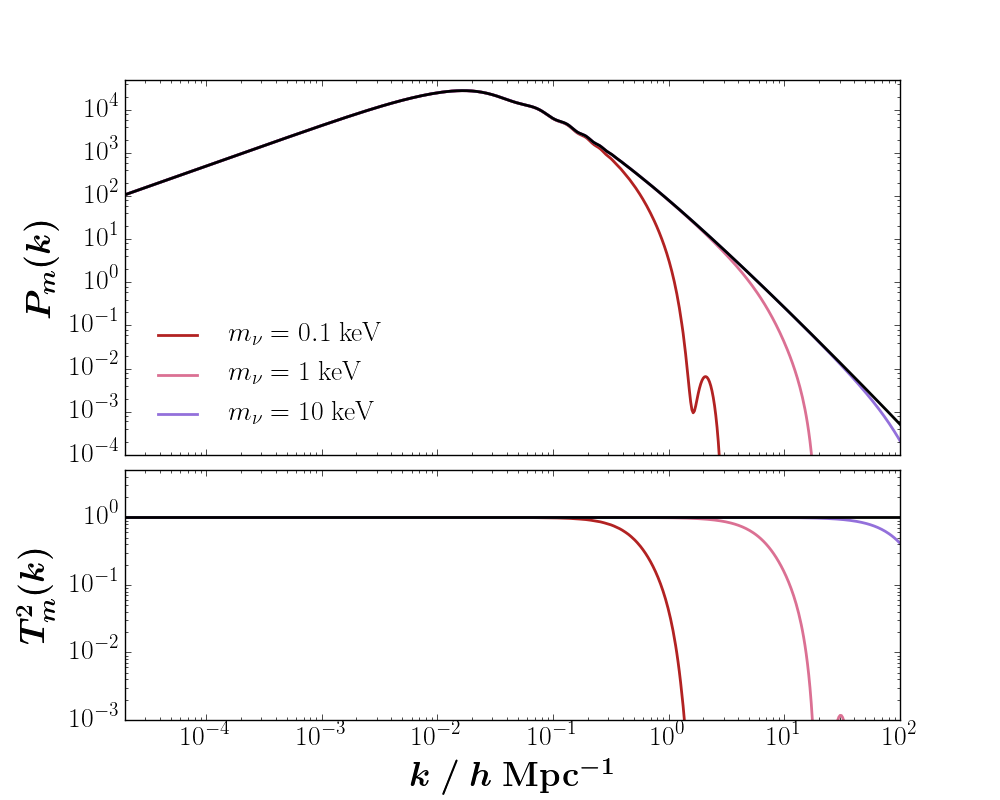
\includegraphics[width=0.4\linewidth]{CosmoParam/Pk_pdm.png}
\caption{Matter power spectrum at $z=0$ and their residual with respect to the standard values of the $\Lambda$CDM model, for varying values of the spectral index (\textbf{top}, see definition in Eq.~\ref{def:Harrison} and Sec.~\ref{sec:primordialps}), expansion rate (\textbf{middle}) and neutrino mass (\textbf{bottom}, see Sec~\ref{sec:mdmps}).}
\label{fig:Pk_cosmo}
\end{center}
\end{figure}


%%%%%%%%%%%%%%%%%%%%%%%%%%%%%%%%%%%%%%%%%%%%%%%%%%%
\subsection{Angular Power Spectrum of Anisotropies}
%%%%%%%%%%%%%%%%%%%%%%%%%%%%%%%%%%%%%%%%%%%%%%%%%%%

\begin{figure}[!]
\begin{center}
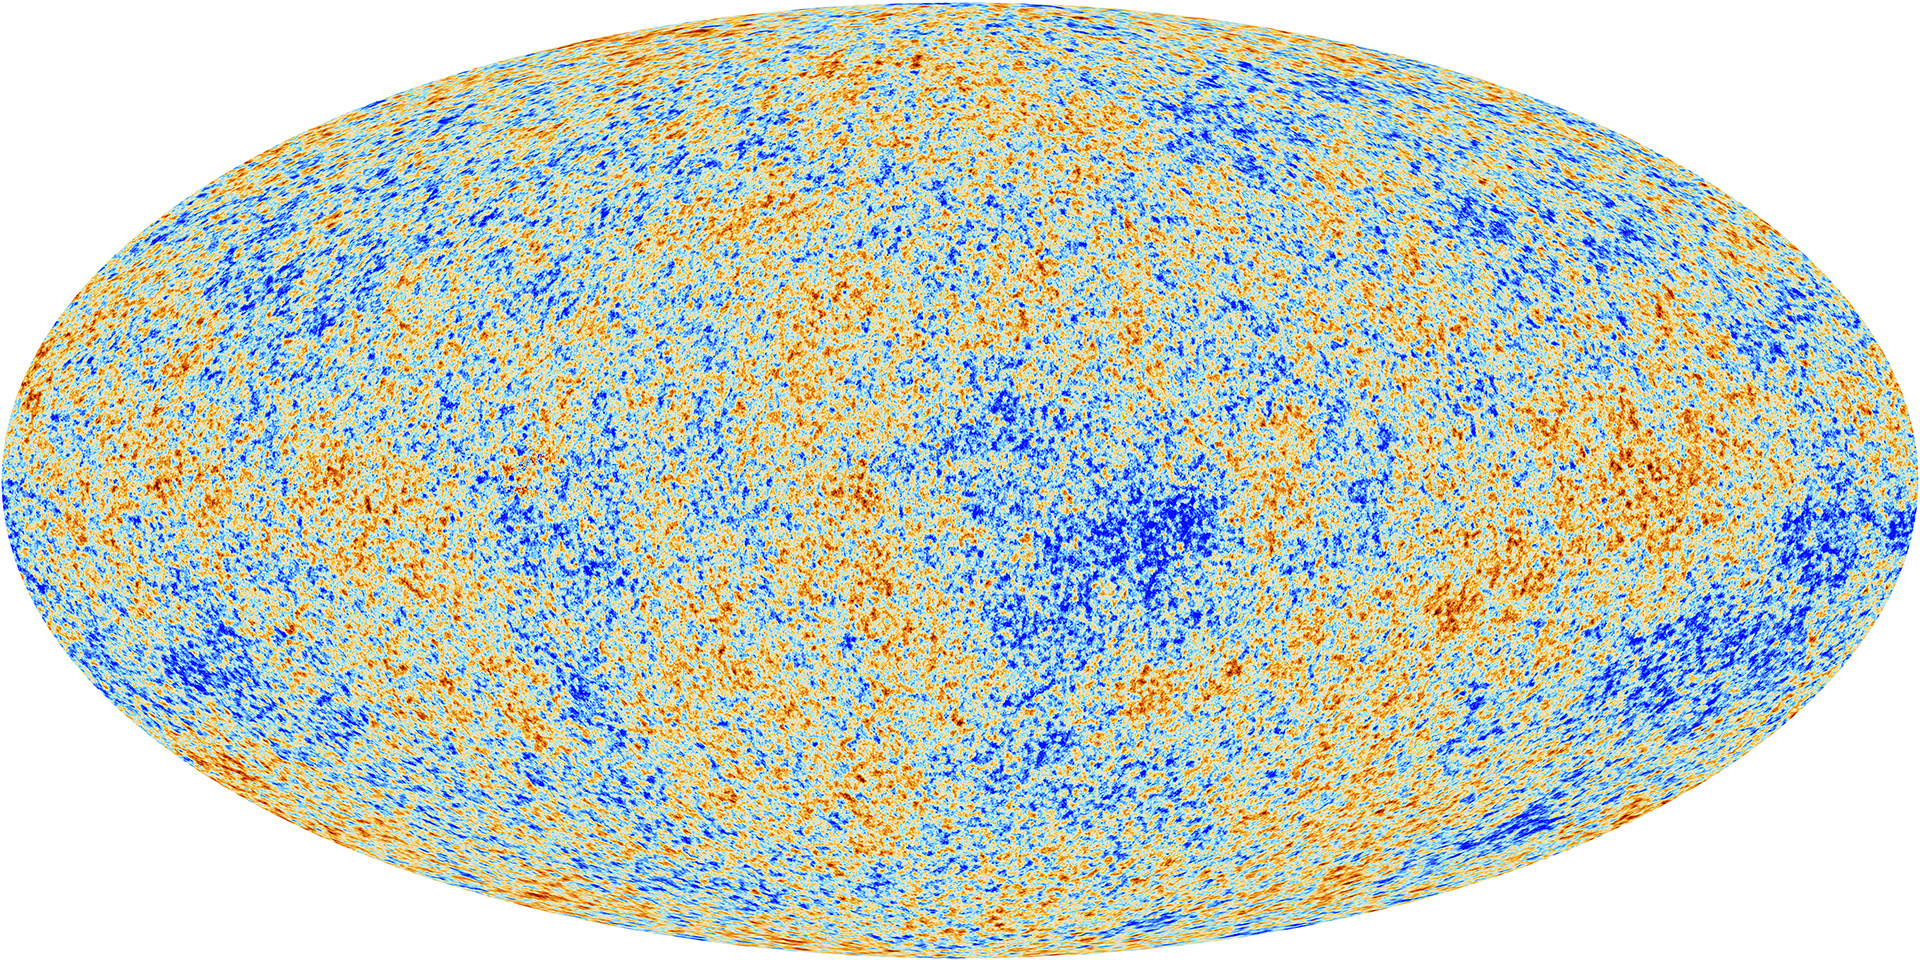
\includegraphics[height=5cm]{Planck_CMB.jpg}~%
\includegraphics[height=5.5cm]{CMB_PS.png}
\caption{\textbf{Left:} Mollweide projection of the CMB temperature anisotropies taken by the Planck spacecraft, year 2. Credit: Planck. \textbf{Right:} Angular power spectrum of temperature anisotropies measured by 5 experiments.}
\label{fig:CMB}
\end{center}
\end{figure}


\subsubsection{Anisotropies in the Temperature Distribution}


Replacing $X$ and $Y$ in expressions~\ref{eq:field_tensor} by the fluctuation in temperature $T_\gamma$ of CMB photons, \\
\begin{equation}
T(\hat{p}, \tau) ~=~ \bar{T}(\tau) ~\left( 1 + \theta(\hat{p}, \tau) \right)
\end{equation} \\ Eq.~\ref{eq:ps_ang_corr} gives the angular auto-correlation power spectrum in temperature fluctuations. The harmonic modes $\mathcal{Y}_{\ell m}$ quantify the temperature fluctuations on solid angle $\Delta \Omega \sim \pi / \ell$. The $00$ harmonic is therefore the CMB temperature averaged over the entire sky: \\
\begin{equation}
a^{\theta \theta}_{00} = 2.72548 \pm 0.00057 ~\mathrm{K} 
\end{equation} \\ as computed in \cite{Fixsen2009}. The first harmonic (dipole) $\ell = 1$ is dominated by the solar system's relative velocity with respect to the CMB, measured in \cite{Lineweaver1996a} to be \\
\begin{equation}
a_{10} =  3.358 \pm 0.023 ~\mathrm{mK}
\end{equation} \\ To study the relative importance of the various harmonics, one can look at the variance of the temperature anisotropies, \\
\begin{equation}
\langle \vert \theta \vert^2 \rangle = \frac{1}{4 \pi} \sum_{\ell = 2}^{\infty} (2 \ell +1) \mathcal{C}_{\ell}
\end{equation} \\ using the orthonormalisation relation of the spherical harmonic base. Just as we defined the variance per log $k$ of the matter power spectrum, which related to the variance in density contrast, we similarly often consider the quantity \\
\begin{empheq}[box=\mymath]{equation}
\mathcal{D}_\ell = \Delta^2_\theta (\ell) = \frac{\ell (\ell + 1)}{2 \pi} \mathcal{C}_\ell
\end{empheq} which quantifies the variance in temperature contrast at a give angular scale $\ell \sim \pi / \Omega$. 


\subsubsection{Link With Matter Power Spectrum}

It can be shown that the temperature anisotropy field can be linked to the overdensity field via
\begin{equation}
\langle \theta(\vec{k}, \hat{p}) \theta^{\ast}(\vec{k}^\prime, \hat{p}^\prime) \rangle = \langle \delta(\vec{k}) \delta^{\ast} (\vec{k}^\prime) \rangle ~\times~ \frac{\theta(k, \hat{k}\cdot \hat{p})}{\delta(k)}~\frac{\theta^{\ast}(k, \hat{k}\cdot \hat{p}^\prime)}{\delta^{\ast}(k)}
\end{equation} which establishes a link between the matter power spectrum and the $\mathcal{C}_\ell$:

\begin{equation}
\mathcal{C}_{\ell} = \frac{2}{\pi} \int_{0}^{\pi} dk~k^2 P(k) ~\left\vert \frac{\theta_{\ell} (k)}{\delta(k)} \right\vert
\end{equation}

\begin{figure}
\begin{center}
\includegraphics[width=0.65\linewidth]{CosmoParam/Cell_ns.png}
%\includegraphics[width=0.45\linewidth]{CosmoParam/Cell_nrun.png}
\includegraphics[width=0.65\linewidth]{CosmoParam/Cell_h.png}
%\includegraphics[width=0.45\linewidth]{CosmoParam/Cell_zreio.png}
\includegraphics[width=0.65\linewidth]{CosmoParam/Cell_mnu.png}
%\includegraphics[width=0.45\linewidth]{CosmoParam/Cell_pdm.png}
\caption{Similar caption to Fig.~\ref{fig:Pk_cosmo} for the temperature fluctuation auto-correlation angular power spectrum.}
\label{fig:Cell_cosmo}
\end{center}
\end{figure}

\clearpage

	\section{Linear Perturbations}
	\label{sec:LP}
	\vspace*{1.5pc}

In this section, I use the Fourier decomposition of small perturbations around mean fields. In the previous chapter, I related the warping of the spacetime curvature to the stress-energy tensor. The relevant quantities for the latter are the density, pressure, and temperature, which we expand into, according to Eqs.~\ref{eq:field} and~\ref{def:fourier}: \\
\begin{equation}
\left\{
\begin{array}{l}
\rho(\vec{x}, \tau) = \bar{\rho} (\tau) \left[ ~1~ + ~ \tilde{\delta}(\vec{k}, \tau) ~ \right] \\
\\
\mathcal{P}(\vec{x}, \tau) = \bar{\mathcal{P}} (\tau) \left[ ~1~ + ~ \tilde{\varpi}(\vec{k}, \tau) ~ \right] \\
\\
T(\vec{x}, \tau) = \bar{T} (\tau) \left[ ~1~ + ~ \tilde{\theta}(\vec{k}, \tau) ~ \right]
\end{array}
\right.
\end{equation} \\ with $\vert \delta \vert, \vert \varpi \vert, \vert \theta \vert \ll 1$ and bulk velocity $u^\mu = (- ds^2)^{-1/2}~dx^\mu \ll 1$ is already an order 1 term since we consider the fluid to be quasi at rest in the comoving coordinates $x^\mu$. I strongly suggest the reader to skip all the way to the summary on page~\pageref{eq:summary_euler} unless he/she is interested in the derivation of linear order perturbations from first principles.

%%%%%%%%%%%%%%%%%%%%%%%%%%%%%%%%%
\subsection{Metric Perturbations}
%%%%%%%%%%%%%%%%%%%%%%%%%%%%%%%%%

\subsubsection{Decomposition}

Perturbing the metric to first order means considering the following space-time metric:
\begin{equation}
\pmb{g} = \pmb{\bar{g}} + \pmb{h}
\end{equation} where $\pmb{\bar{g}}$ is the metric describing the background, \textit{i.e.} the FRW metric defined in Eq.~\ref{eq:RWmetric}. In cartesian coordinates, its contravariant components are \\
\begin{equation}
\bar{g}_{\mu \nu} = a^2(t) \times \eta_{\mu \nu}
\end{equation} \\ The perturbed metric $\pmb{h}$ is such that $\vert \vert h_{\mu \nu} \vert \vert \ll 1$. In its most general form, its contravariant components can be written as \\
\begin{equation}
\label{eq:metric_perturb}
h_{\mu \nu} = a^2(t) \times 2~\left(
\begin{array}{cc}
	h_t & \vec{h}\\
	\vec{h} & \pmb{h_s}
\end{array}
\right)
\end{equation} \\ The $2$ comes from the development at first order (square term). The above expression features a scalar $h_t$ for the time component, spatial vectors $\vec{h}$ and a rank 2 symmetric spatial tensor $\pmb{h_s}$. Vectors can always be decomposed into a curl-free and a divergence-free component, so we may decompose the vector modes as a radial and a transverse term $\vec{h} = \vec{h}^{\parallel} + \vec{h}^{\bot}$ with
\begin{equation}
\left\{
\begin{array}{l}
\vec{\nabla} \times \vec{h}^{\parallel} = \vec{0}\\
\\
\vec{\nabla} \cdot \vec{h}^{\bot} = 0
\end{array}
\right.
\end{equation} The first (curl-free) component only requires a single scalar to be determined (its direction). The second (divergence-free) component has two degrees of freedom since $\vec{h}^{\bot}$ can be expressed in any basis whose vectors are in the plane normal to $\vec{h}^{\parallel}$. A similar decomposition applies to the spatial tensor, which we expand into a radial, a transverse and a tensoral term $\pmb{h_s} = \pmb{h_s}^{\parallel} + \pmb{h_s}^{\bot} + \pmb{h_s}^T$, where
\begin{equation}
\left\{
\begin{array}{ll}
h^{\parallel}_{ij} = \left(\cfrac{\vec{\nabla}_i \vec{\nabla}_j }{3} ~g_{ij}~ \nabla^2 \right) h^{\parallel}_0 & \text{where}~h^{\parallel}_0 \in \mathbb{R} ~\text{is a scalar}\\
\\
h^{\bot}_{ij} = \vec{\nabla}_i h^{\bot}_j + \vec{\nabla}_j h^{\bot}_i & \text{where}~ h^{\bot}_i ~\text{are the components of a divergence-free spatial vector}
\end{array}
\right.
\end{equation} Similar to the vector decomposition, the $\parallel$ and $\bot$ components of tensor $\pmb{h}$ gives an additional 1 scalar and 2 vector degrees of freedom. Because $\pmb{h}$ has to be traceless, this leaves only two independant degrees of freedom to define the tensoral part of $\pmb{h}^T$, which are typically denoted $h^{+}$ and $h^{\times}$ and correspond to the two polarization states of gravitational waves. This gives us a total of 9 degrees of freedom, in addition to a scalar degree of freedom $h_s$ to which we can multiply $\pmb{h_s}$ for a total of 10:
\begin{equation*}
h_t, ~h_s, ~\vec{h}^{\parallel},
~\left(
\begin{array}{c}
\vec{h}^{\bot}_{+}\\
\vec{h}^{\bot}_{\times}
\end{array}
\right), ~h^{\parallel}_0, 
~\left(
\begin{array}{c}
h^{\bot}_{+}\\
h^{\bot}_{\times}
\end{array}
\right), 
~\left(
\begin{array}{c}
h^{T}_{+}\\
h^{T}_{\times}
\end{array}
\right)
\end{equation*}

\subsubsection{Gauge Freedom}
\label{sec:gauge}

At the linear level, rotational modes decouple from the others. We can thus only consider the scalar degrees of freedom instead of the total 10: $h_t$, $h_s$, $\vec{h}^{\parallel}$ and $h^{\parallel}_0$. However, of those 4, only two are physical. The other two depend on our choice of coordinates. This is known as \textbf{gauge freedom}. In electromagnetism, the electric potential $V$ can be defined with any scalar offset $V + \xi$ since only the Laplacian (contravariant derivative) is a physical quantity (the electric charge density $\rho_e$) by virtue of the Poisson equation $\nabla^2 V = \rho_e / \epsilon_0 = \nabla^2 ( V + \xi )$. For analogous reasons, only 2 of the 4 scalars enumerated are physical quantities. The other two are mute since they depend on the choice of a coordinate system. Several gauges can be chosen. One that is conveniant for first order perturbations is setting $\vec{h}^{\parallel} = 0$ and $h^{\parallel}_0 = 0$, known as the \textbf{conformal Newtonian gauge}. Conformal because the time coordinate is conformal time and Newtonian because the two remaining scalar degrees of freedom correspond to the Newtonian gravitational potential (such that $\nabla^2 \psi = 4 \pi G \rho$). Because of this, it is conventional to set
\begin{equation*}
\begin{array}{rr}
h_t \mapsto & \psi\\
h_s \mapsto & -\phi
\end{array}
\end{equation*} so that the line element in this perturbed metric in this gauge can be written \\
\begin{empheq}[box=\mymath]{equation}
\label{eq:perturbed_metric}
ds^2 = a^2(t) ~\left( -(1 + 2 \psi) ~d\tau^2 + (1 - 2 \phi ) ~\delta_{ij} dx^i dx^j \right)
\end{empheq} \\ In this perturbed metric, the particle's individual 4-momentum is
\begin{equation}
\pmb{P} = \left[ ~(1+\psi) \epsilon, (1-\phi) \vec{q} ~ \right]
\end{equation} with $\vec{q} = q \hat{q} = a \vec{p} = \vec{p}/T$ where $\vec{p}$ is the particle's \emph{proper} momentum as measured by an observer stationary in the comoving coordinate system and $\epsilon(q) = a E = E/T = \sqrt{a^2 m^2 + q^2}$. It is useful to use $\vec{q}$ and $\epsilon$ instead of $\vec{p}$ and $E$ since in absence of metric perturbations ($\phi = 0 = \psi$), these quantities are not redshifted.\\ 


\subsubsection{Einstein Equations}

We can use the perturbed metric in expression~\ref{eq:perturbed_metric} to compute the Riemann curvature tensor, its Ricci contraction and the trace, and link the subsequent Einstein tensor to the perturbed energy-stress tensor \\
\begin{equation}
\pmb{T} = \bar{\pmb{T}} ~\left[ 1 + \pmb{\Pi} \right] = (\rho + \mathcal{P}) \pmb{u} \otimes \pmb{u} + \mathcal{P}\pmb{g} + \pmb{\Sigma}
\end{equation} \\ with $\pmb{\Sigma}$ the shear stress tensor and $\vert \vert \pmb{\Pi} \vert \vert \ll 1$, which we can also decompose into scalar, vector and tensor modes each evolving independantly of one another at linear order. Isolating the scalar modes only of $\pmb{\Pi}$ (left-hand terms of Eq.~\ref{sys:et}) and equating them with those of the Einstein tensor (right-hand terms of Eq.~\ref{sys:et}), one can show that \\
\begin{equation}
\label{sys:et}
\left\{
\begin{array}{lcl}
4 \pi G a^2~ \bar{\rho} \tilde{\delta} &=& - k^2 \tilde{\phi} - 3 H \left( \dot{\tilde{\phi}} + H \tilde{\psi} \right)\\
\\
4 \pi G a^2~ \tilde{\varpi} &=& \ddot{\tilde{\phi}} + H \left( \dot{\tilde{\psi}} + 2 \dot{\tilde{\phi}} \right) + \left( 2 \dot{H} + H^2 \right) \tilde{\psi} + \cfrac{k^2}{3} \left( \tilde{\phi} - \tilde{\psi} \right) \\
\\
4 \pi G a^2~ \left( \bar{\rho} + \bar{\mathcal{P}} \right) \tilde{\vartheta} &=& \dot{\tilde{\phi}} + H \tilde{\psi}\\
\\
4 \pi G a^2~ \left( \bar{\rho} + \bar{\mathcal{P}} \right) \tilde{\sigma} &=& - \cfrac{k^2}{3} \left( \tilde{\phi} - \tilde{\psi} \right)\\
\end{array}
\right.
\end{equation} \\ with $\tilde{\vartheta} = \vec{\nabla} \cdot \vec{v} = -i k^i \tilde{v}_i$ the divergence of the coordinate velocity $v_i = \dot{x_i}$ and \\
\begin{equation}
\left( \bar{\rho} + \bar{\mathcal{P}} \right) \tilde{\sigma} \doteq - \left( \cfrac{k_i}{k}\cfrac{k_j}{k} - \cfrac{\delta_{ij}}{3} \right) \tilde{\Sigma}^{ij}
\end{equation} \\ the anisotropic stress. All dotted expressions are differentiated with respect to conformal time. Solving system~\ref{sys:et} requires linking the left-hand terms to the Boltzmann moments. 


%%%%%%%%%%%%%%%%%%%%%%%%%%%%%%%%%%%%%%%%%%%%%%%%%
\subsection{Perturbing the Boltzmann Equilibrium}
%%%%%%%%%%%%%%%%%%%%%%%%%%%%%%%%%%%%%%%%%%%%%%%%%

To get the stress-energy tensor terms, we can take its general covariant expression in Eq.~\ref{eq:nrj_general}, this time the metric trace being $(-g)^{-1/2} = a^{-4} (1-\psi+3\phi)$ ($= a^{-4}$ in absence of perturbations). Using the comoving momentum and energy we defined in Sec.~\ref{sec:gauge}, we can identify using the quantities defined in expression~\ref{eq:moments} the perturbed energy density, flux and stress as being \\
\begin{equation}
\label{sys:perturb_stress_energy}
\left\{
\begin{array}{l}
T^0_0 = -\cfrac{1}{a^4} \displaystyle \int \cfrac{d^3q}{(2\pi)^3}~ \epsilon~ f(\vec{x}, \vec{q}, \tau)\\
\\
T^0_i = \cfrac{1}{a^4} \displaystyle \int \cfrac{d^3q}{(2\pi)^3}~ q_i~ f(\vec{x}, \vec{q}, \tau)\\
\\
T^i_j = \cfrac{1}{a^4} \displaystyle \int \cfrac{d^3q}{(2\pi)^3}~ \cfrac{q^i q_j}{\epsilon}~ f(\vec{x}, \vec{q}, \tau)
\end{array}
\right.
\end{equation} \\ The distribution function is tracked by the Boltzmann equation which we can rewrite with the comoving quantities: \\
\begin{equation}
\label{eq:boltzmann_reference}
\left[ \partial_\tau + \left( \dot{\vec{x}} \vec{\nabla}_{\vec{x}} \right) + \left( \dot{\vec{q}} \vec{\nabla}_{\vec{q}} \right) \right]~f = \mathcal{C}[f]
\end{equation}

\subsubsection*{Boltzmann Hierarchy}

We may decompose $f(\vec{x}, \vec{q}, \tau) = f_0(q) + \Phi(\vec{x}, \vec{q}, \tau)$ into an equilibrium distribution function $f_0 (q)$ given by Eq.~\ref{eq:fermibose} function of $q = \vert \vec{q} \vert$ only because of homogeneity and isotropy
\begin{equation}
\label{eq:dist_eq_0}
f_0(q) = \frac{\beta}{e^{\alpha (q-\xi)} \pm 1}
\end{equation} and an off-equilibrium perturbation in the distribution function $\Phi(\vec{x}, \vec{q}, \tau)$ such that $\vert \Phi/f_0 \vert \ll 1$. In Eq.~\ref{eq:dist_eq_0} above, $\xi = \mu / T_\nu$ is the comoving chemical potential of the generic particle of temperature\footnote{I use $T_\nu$ as the reference temperature since photons get reheated by $e^{\pm}$ pair annihilation, whereas neutrinos are approximately not} $T = \alpha T_\nu$ and $0 \leqslant \beta \leqslant 1$ is a factor accounting for particles which are not produced in thermal equilibrium, which is the case for sterile neutrinos. Expanding out the collisionless Boltzmann equation for non-interacting matter (dark matter, neutrinos), the linear order corrections follow
\begin{equation}
\label{eq:perturb_boltz}
\frac{\partial \Phi}{\partial \tau} + \frac{q^i}{\epsilon}\frac{\partial \Phi}{\partial x^i} + \frac{d q}{d \tau} \frac{\partial f_0}{\partial q} = 0
\end{equation} In Fourier space, with $\vec{q} = q \hat{q}$, $\vec{p} = p \hat{p}$, $\vec{k} = k \hat{k}$ and $\mu = \hat{q} \hat{k}$ the cosine of the angle between them (not the chemical potential !), 
\begin{equation}
\label{eq:perturb_boltz_fourier}
\frac{\partial \tilde{\Phi}}{\partial \tau} + i \frac{qk\mu}{\epsilon} \tilde{\Phi} + \left[ q \dot{\tilde{\phi}} - i \epsilon k \mu \tilde{\psi} \right] \frac{\partial f_0}{\partial q} = 0
\end{equation} where the energy gradient term comes from the geodesic equation using the 4-momentum (see Eq.~\ref{eq:geodesic_p}) $\partial_\tau P^\alpha = 1/m~ \Gamma^\alpha_{\mu \nu} p^\mu P^\nu$. For cold dark matter and neutrinos, one can deduce the density contrast $\tilde{\delta}$ and velocity divergence $\tilde{\vartheta} = i k^i \tilde{v}_i$ from Eq.~\ref{sys:perturb_stress_energy}:
\begin{equation}
\label{eq:boltmo}
\left\{
\begin{array}{l}
\bar{n} \tilde{\delta} = \displaystyle \int \cfrac{d^3 q}{(2 \pi a)^3} ~\tilde{\Phi}\\
\\
\bar{n} \tilde{\vartheta} = \displaystyle \int \cfrac{d^3 q}{(2 \pi a)^3} ~ \cfrac{qk\mu}{\epsilon} ~\tilde{\Phi}
\end{array}
\right.
\end{equation} with $\bar{n} = a^{-3}/2\pi~ \displaystyle\int d^3 q f_0$ the mean density. For non-relativistice matter, higher orders of $(q/\epsilon)^{n \geqslant 2}$ are all negligeable, and so only the zeroth and first moments of Eq.~\ref{eq:perturb_boltz_fourier} drive the perturbations for non-interacting non-relativistic matter: the continuity and Euler equations. Dropping the tilda symbols,  \\
\begin{empheq}[box=\mymath]{equation}
\left\{
\begin{array}{l}
\dot{\delta} + \vartheta - 3 \phi = 0\\
\dot{\vartheta} + H \vartheta - k^2 \psi = 0
\end{array}
\right.
\end{empheq} \\

Since the $\vec{q}$ dependance of  $\tilde{\Phi}(k, q, \mu, \tau)$ is only function of its relative alignement with the mode vector, we can decompose it into Legendre series:
\begin{equation}
\tilde{\Phi} (k, \mu, q, \tau) = \sum_{n=0}^{\infty} (-i)^n (2n + 1) ~\Psi_n (k, q, \tau)~ \mathbb{P}_n (\mu)
\end{equation} where the Legendre moments of $\Phi$ are
\begin{equation}
\label{def:lengendre_moment}
\Psi_n (k, q, \tau) = \frac{1}{2 (-i)^n} \int_{-1}^{+1} d\mu~ \tilde{\Phi} (k, \mu, q, \tau)~\mathbb{P}_n (\mu)
\end{equation} and 
\begin{equation}
\mathbb{P}_n(\mu) \doteq \frac{1}{2^n n \!} \frac{d^n}{d \mu^n} \left[ (\mu^2 - 1)^n  \right]
\end{equation} are the Legendre polynomials of degree $n$. The energy density and pressure can both be expressed in terms of moments of the monopole $\Psi_0$, while the dipole $\Psi_1$ and quadrupole moments $\Psi_2$ give the velocity divergence and anisotropic stress respectively: \\
\begin{equation}
\label{sys:te}
\left\{
\begin{array}{l}
\tilde{\delta \rho} = \cfrac{1}{a^4} \displaystyle \int \cfrac{d^3 q}{(2 \pi)^3}~ \epsilon \Psi_0\\
\\
\tilde{\delta \mathcal{P}} = \cfrac{1}{3 a^4} \displaystyle \int \cfrac{d^3 q}{(2 \pi)^3}~ \epsilon \left(\cfrac{q}{\epsilon} \right)^2 \Psi_0\\
\\
\left( \bar{\rho} + \bar{\mathcal{P}} \right) \tilde{\vartheta} = \cfrac{k}{a^4} \displaystyle \int \cfrac{d^3 q}{(2 \pi)^3}~ \epsilon \left(\cfrac{q}{\epsilon} \right) \Psi_1\\
\\
\left( \bar{\rho} + \bar{\mathcal{P}} \right) \tilde{\sigma} = \cfrac{2}{3 a^4} \displaystyle \int \cfrac{d^3 q}{(2 \pi)^3}~ \epsilon \left(\cfrac{q}{\epsilon} \right)^2 \Psi_2
\end{array}
\right.
\end{equation} \\ which now closes the system in Eq.~\ref{sys:et}.\\

Integrating Eq.~\ref{eq:perturb_boltz_fourier} as per the multipolar Legendre expansions of $\Phi$ yields the so-called \textbf{Boltzmann hierarchy}:
\begin{empheq}[box=\mymath]{equation}
\label{sys:hierarchy_boltz}
\left\{
\begin{array}{l}
\dot{\Psi}_0 = - \cfrac{qk}{\epsilon} \Psi_1 - \dot{\phi} \cfrac{d f_0}{d \ln q} \\
\\
\dot{\Psi}_1 = \cfrac{qk}{3\epsilon} (\Psi_0 - 2 \Psi_2) - \cfrac{\epsilon k}{3 q} \psi \cfrac{d f_0}{d \ln q}\\
\\
\dot{\Psi}_{n \geqslant 2} = - \cfrac{qk}{(2n+1)\epsilon} \left[ n \Psi_{n-1} - (n+1) \Psi_{n+1} \right]
\end{array}
\right.
%\end{equation}
\end{empheq} A Boltzmann solver code like \texttt{CAMB}, truncating the Boltzmann hierarchy at $n \leqslant 6$ and using $\sim 10^3$ bins of comoving momentum is sufficient to compute the matter power spectrum with percent level accuracy.


\subsection{Vlasov Equations}

Linking Systems~\ref{sys:et} and \ref{sys:te} gave the 4 diagonal non-trivial equation equivalents of the Poisson equation, which simply translates the divergence-free nature of the Einstein tensor, the general relativity equivalent of the divergence-free nature of the gravitational field in the Newtonian limit. These may seem intimidating at first glance, but they simply exhibit how the density, pressure, velocity divergent and anisotropic stress are linked to the metric, and thereby to each other. For most species in the Universe, they can be simplified drastically. For non-relativistic matter, only the monopolar Legendre moment $\tilde{\Psi}_0$ from Eq.~\ref{def:lengendre_moment} is relevant, and thus there is neither velocity divergence nor anisotropic stress, as expected, and thus the fourth component in the \ref{sys:et} system shows that the two scalar potentials are equal $\phi = \psi$, which in turn drastically simplifies the first and second components, which in fact reduce to  the Fourier modes of the Possion equation perturbed at first order on $\phi$ and $\delta$ \\
\begin{equation}
\frac{k^2}{a^2} \tilde{\phi} = 4 \pi G a^2 \bar{\rho}~ \tilde{\delta}
\end{equation} \\ and the second Friedmann equation at first order perturbations on $\mathcal{P}$ respectively; which by some trivial manipulation yields the Euler equation, assuming an equation of state similar to Eq.~\ref{eq:eos}, since $\varpi = w \delta$. This leaves us yearning for the continuity equation, which can simply be derived from the zeroth moment of the (collisionless) Boltzmann equation in expression~\ref{eq:boltzmann_reference} and identifying the moments defined in the~\ref{eq:boltmo} expressions:\\
\begin{equation}
\begin{array}{c}
\displaystyle \int \cfrac{d^3 q}{(2 \pi)^3 a^4}~~~\left\{ \cfrac{\partial f}{\partial \tau} + \frac{q^i}{\epsilon}\cfrac{\partial x^i}{\partial x^i} + \dot{q} \cfrac{\partial f}{\partial q} = 0 \right\} \\
\\
\Rightarrow\\
\\
\dot{n} + \cfrac{-ik^i}{a} (n v_i) + 3 \left( H - \dot{\phi}\right) = 0 \\
\end{array}
\end{equation} \\ which yields $d_\tau (\bar{n} a^3) = 0$ for zero order perturbations (which is what we derived in Ch.~\ref{chap:cosmology} for the background evolution of non-relativistic matter $\bar{n} \propto \bar{\rho} \propto a^{-3}$) \\
\begin{equation}
\dot{\delta} + \vartheta + 3 \dot{\phi} = 0
\end{equation} \\ These are only valid in the case of a non-interacting fluid. Baryons are coupled to photons up until the freeze-out of baryon acoustic oscillations, and so the collision term $\mathcal{C}[f_b, f_\gamma]$ must not be neglected. One could get the expression from particle physics, setting equilibrium between baryons and photons via Compton scattering, which leads to the blue term in Eq.~\ref{eq:summary_euler} where $\dot{\tau}_{\mathrm{Compton}}$ is the rate of Compton scattering (optical depth) and \\
\begin{equation}
\label{eq:tcl}
\frac{1}{R} \doteq \frac{4 \rho_{\gamma, 0}}{3 \rho_{b, 0}}
\end{equation} \\ and $\Theta_{0,1,2}$ the monopole, dipole and quadrupole Legendre moments for the photon temperature fluctuations $\theta$. \\

Finally, taking the first moment of the Boltzmann equation and identifying the~\ref{eq:boltmo} expressions and neglecting all superior orders in $(q/\epsilon)^{n \geqslant 2}$ yields \\

\begin{equation}
\begin{array}{c}
\displaystyle \int \cfrac{d^3 q}{(2 \pi)^3 a^4}~\cfrac{q\hat{q}^i}{\epsilon}~~~\left\{ \cfrac{d f}{d\tau} = 0 \right\} \\
\\
\Rightarrow \\
\\
\dot{\mathcal{J}} + 4 H \mathcal{J} + n~ik \psi = 0 \\
\end{array}
\end{equation} with $\mathcal{J}^i = n v^i$ the current. This equation has no zero-order part, whereas the first order perturbations for radiation ($\mathcal{J}_r = \rho_r$) yields

\begin{equation}
\dot{v}^j + H v^j + ik~\psi = 0
\end{equation} which is Euler's linearly-perturbed equation for radiation.

\subsection*{Summary}

We've derived the fully linearly perturbed Einstein equation in the perturbed FRW metric in the conformal Newtonian gauge, which allowed us to isolate the evolution of the scalar modes independantly of the vector and tensor modes. Using the Boltzmann equation, we've linked the Einstein and stress-energy tensors with the set of 4 Einstein Field Equations~\ref{sys:et} and~\ref{sys:te}. We've also derived the continuity and Euler equations from the moments of the Boltzmann equation, just as one would do in classical statistical physics to get the Vlasov-Poisson system. For photons, massless neutrinos and any relativistic dark matter, this whole set of equations is necessary to solve the linear perturbations in $\theta_r$ and $\delta_r$.\\

For non-relativistic matter, the equations simplify drastically and become identical to linearly perturbing the Vlasov-Poisson equations around density, bulk velocity, pressure and gravitational potential for a fluid at rest in the comoving coordinate system. In summary, denoting index $m$ for non-reltivistic matter and $r$ for massless radiation, and dropping the tilde, each linear Fourier mode evolves as: \\


\begin{empheq}[box=\mymath]{equation}
\label{eq:summary_euler}
\left\{
\begin{array}{lcl}
\dot{\delta}_m + \vartheta_m &=& - 3 \dot{\phi}\\
\\
\dot{v}_m + H v_m &=& -ik \psi ~{\color{blue} + \cfrac{\dot{\tau}}{R} \left( 3 i ~\Theta_1 \right) }\\
\\
\dot{\theta}_r + ik \mu ~\theta_r &=& \dot{\phi} - ik \mu ~\psi ~{\color{blue} - \dot{\tau} \left( \Theta_0 - \theta + \mu v_b - \frac{1}{2} \mathbb{P}_2(\mu) \Pi \right)}
\end{array}
\right.
%\end{equation} \\
\end{empheq} \\

where the blue term only applies for baryons and photons in the strong coupling limit, and taking the Einstein equations with no anisotropic stress \\

\begin{empheq}[box=\mymath]{equation}
\label{eq:summary_poisson}
\left\{
\begin{array}{lcl}
k^2 \phi + 3H \left( \dot{\phi} - H \psi \right) &=& 4 \pi G a^2 \left( \rho_m \delta_m + 4 \rho_r \Theta_{0} \right)\\
\\
k^2 \left( \phi + \psi \right) &=& -32 \pi G a^2~ \rho_r \Theta_{2}
\end{array}
\right.
%\end{equation} \\
\end{empheq} \\

Keep in mind that to accurately model the evolution of neutrino perturbations to the percent level, a Boltzmann solver like \texttt{CAMB} or \texttt{CLASS} is necessary to account for the anisotropic stress and non-vanishing velocity divergence. They use the Boltzmann hierarchy displayed in Eq.~\ref{sys:hierarchy_boltz}. That isn't necessary to get a glimpse of what kind of behaviour to expect from neutrino perturbations. In what follows, I make use of the simplified Vlasov and Poisson Equations~\ref{eq:summary_euler} and~\ref{eq:summary_poisson} to have a coarse-grain apprehension of the impact of non-cold dark matter on the power spectrum.

\clearpage
	
	\section{Solving Neutrino Linear Perturbations}
	\label{sec:CAMB}
	\vspace*{1pc}


The Code for Anisotropies in the Microwave Background, or \texttt{CAMB}\footnote{\url{http://camb.info}} \citep{Lewis2000} is a
numerical Boltzmann code written in Fortran 90. It is a parallelized line-of-sight integration code which is widely used (and thus tested) to calculate not only
the lensed cosmic microwave background temperature and polarization spectra but also linear matter power spectra for different
species of particles (in our case baryons, dark matter and sometimes neutrinos). The Cosmic Linear Anisotropy Solving System, or \texttt{CLASS}\footnote{\url{http://class-code.net/}} \citep{CLASS} is a newer code  similar to \texttt{CAMB} with additional features such as the option of inputing a non-cold dark matter particle momentum distribution function, which was crucial for one of the projects I managed, involving resonantly-produced sterile neutrinos as a cool dark matter candidate particle (see Sec.~\ref{sec:rpsn_intro}).



%%%%%%%%%%%%%%%%%%%%%%%%%%%%%%%%%%%%%%%%%%%
\subsection{Power Spectrum of $\Lambda$CDM}
%%%%%%%%%%%%%%%%%%%%%%%%%%%%%%%%%%%%%%%%%%%

\subsubsection{Initial Conditions}
\label{sec:primordialps}

The 10 small perturbation variables ($\delta_{\mathrm{dm}, b, \nu}, v_{\mathrm{dm}, b, \nu}, \theta_{\gamma, \nu}, \phi, \psi$) obey the set of 10 first-order differential equations~\ref{eq:summary_euler}~\ref{eq:summary_poisson}. In principle, solving for the perturbations requires initial conditions for all 10 of them. However, in practice, when one assumes conformal times early enough so that any relevant $k$ mode verify $k \tau \ll 1$, a lot of simplifications can be taken advantage of to relate all of the required initial conditions to those on $\phi$ alone. Indeed, perturbations which have a wavelength $\lambda \sim k^{-1}$ at early times very large compared to the length scale at which causal physics applies (the horizon), all time derivative terms ($\propto \tau^{-1}$) are larger than gradient terms ($\propto k$) by a factor of order $\mathcal{O}(1/k\tau)$ which is large by assumption. Therefore the 8 Boltzmann equations in~\ref{eq:summary_euler} boil down to only the following 4\footnote{massless neutrinos obey the first involving its temperature monopole. The second involving their density only apply to the massive case} under this assumption:

\begin{equation}
\left\{ \begin{array}{ll}
\dot{\Theta}_{0, r} + \dot{\phi} = 0 & r \in \lbrace \gamma, \nu \rbrace \\
\\
\dot{\delta}_m - 3 \dot{\phi} = 0 & m \in \lbrace \mathrm{dm}, b, \nu \rbrace
\end{array}
\right.
\end{equation} \\

All velocity terms are smaller by a $\mathcal{O}(k \tau)$ factor, as are higher multipolar moments of the temperature distribution. For the baryon population, the tight coupling limit is valid, meaning the velocity term is exactly linked to the temperature dipole, set by the large value of $\dot{\tau}_{\mathrm{Compton}}$ (see Eq.~\ref{eq:tcl}): \\

\begin{equation}
v_b + 3 i \Theta_{1, \gamma} = 0
\end{equation} \\

Combining the Einstein equations (Eq.~\ref{eq:summary_poisson}) at very early times yield a second-order differential equation on the gravitational potential \\

\begin{equation}
\tau \ddot{\phi} + 4 \dot{\phi} = 0 
\end{equation} which admits 2 solutions if we assume $\phi \sim \tau^p$ is polynomial: $\phi \propto \tau^{-3} + \tau^0$. The first mode is decaying so even if it is excited at early times, it soon vanishes with respect to the constant mode. This mode yields $\dot{\phi} = 0 \Rightarrow \dot{\theta} = 0 \Rightarrow \theta = \mathrm{cst}, \delta = \mathrm{cst}, \delta_b = \mathrm{cst}$ and so in summary, if we equal both massless neutrino and photon temperature monopoles at early times: \\

\begin{equation}
\left\{
\begin{array}{l}
\Theta_{0, \nu} (k, \tau_{\mathrm{ic}}) = \Theta_{0, \gamma} (k, \tau_{\mathrm{ic}}) \doteq \Theta_{0} (k, \tau_{\mathrm{ic}}) \\
\\
\phi_0 (k, \tau_{\mathrm{ic}})  = 2 \Theta_{0} (k, \tau_{\mathrm{ic}}) \\
\\
\delta_m (k, \tau_{\mathrm{ic}}) - 3 \Theta_0 (k, \tau_{\mathrm{ic}}) = A
\end{array}
\right.
\end{equation} \\

So, solving for perturbations only requires the knowledge of 3 constants: $\Theta_0, \phi_0 ~\&~ A$, the last one of which depends on the nature of the primordial perturbations: \\

\begin{itemize}

\item[$\bullet$] adiabatic perturbations: $A = 0$ \\

\item[$\bullet$] isocurvature perturbations: $A \neq 0$ \\

\end{itemize}

 
Adiabatic perturbations feature a constant matter-to-radiation ratio everywhere since

\begin{equation*}
\frac{n_{\mathrm{dm}}}{n_{\gamma}} = \frac{n_{\mathrm{dm}}^0 (1+\delta)}{n^0_{\gamma} (1+3\Theta_0)} \simeq \frac{n^0_{\mathrm{dm}}}{n^0_{\gamma}} (1+\underbrace{\delta-3\Theta_0}_{0~ \text{if adiabatic}})
\end{equation*} and likewise for the baryon-to-entropy ratio $\eta_b = n_b / n_\gamma$. The standard model of cosmology assumes adiabatic scale invariant initial conditions. As such, all perturbations can be solved with the knowledge of a single function: the \textbf{primordial power spectrum} $\vert \phi(\vec{k}, \tau_{\mathrm{ic}} \ll \tau_{\mathrm{eq}}) \vert^2$ where $k \tau_{\mathrm{eq}} \simeq 1$. It is assumed to follow the expression for the Harison-Zel'dovich initial power spectrum (set by inflation) \\

\begin{empheq}[box=\mymath]{equation}
\label{def:Harrison}
k^3 ~ \left\vert \phi_{s,t}(\vec{k}, \tau_{\mathrm{ic}}) \right\vert^2 \simeq \mathcal{A}_{s,t} ~ k^{n_{s,t} - 1}
%\end{equation}
\end{empheq} \\
where $n=1$ for scale invariance and the $s$ and $t$ subscripts stand for the scalar and tensor modes of perturbations. As I've specified earlier in this chapter, I only consider scalar modes. I shall also mention that I am working under the gaussian assumption, meaning that $\phi$ is chosen such that its variance is its power spectrum $\vert \phi \vert^2$.\\

The assumption of decoupled modes at very early times enabled us to set the evolution of perturbations in density, velocity (and its divergence), temperature multipoles and gravitational potentials to solely the power spectrum of $\phi$, which is fully determined by an amplitude $\mathcal{A}_s$ and a spectral index $n_s$ for scalar modes, under the axiom that initial conditions are adiabatic and scale invariant. The CMB for instance can be fully determined by $\mathcal{A}_s$, $n_s$, the running of the scalar spectral index $d ns / d \ln k$, the ration of scalar to tensor power spectra $r$ and the optical depth to reionization $\tau_{\star}$. I should mention that although isocurvature pertubations are seldom used, these lead to 
\begin{equation}
\Theta_{1, r} = \frac{i v_m}{3} = - \frac{k \phi}{6 a H}
\end{equation} and so the power spectrum of $\phi$ determines each $k$ mode of all perturbations of interest as well.\\

In Sec.~\ref{sec:PS}, I introduced the formal definitions of power spectra for temperature and density fluctuations in radiation and density distributions. I've shown how they relate to the variance in their field and help quantify inhomogeneities and anisotropies. In the present Sec.~\ref{sec:CAMB}, I detail how the mass of neutrinos and dark matter particles impact the power spectrum through their free-streaming. 


\subsubsection{Pure Cold Dark Matter}


\begin{figure}
\begin{center}
\includegraphics[width=0.8\columnwidth]{Pcdm_ic.png}
\caption{Power spectra of the matter distribution at $z=0$ in a standard $\Lambda$CDM model (thick solid black curve) and a pure $\Lambda$HDM model (thick solid red curve). The CDM transfer function $\mathcal{T}(k)$ defined in Eqs.~\ref{def:cdm_tf},\ref{eq:cdm_tf} is the ratio (square rooted) between the CDM power spectrum and that of the scalar modes of linear perturbations given by Eq.~\ref{def:Harrison} (grey dashed curve). The HDM transfer function $T(k)$ is the (square rooted) ratio between the HDM and CDM power spectra.}
\label{fig:initialpwrspc}
\end{center}
\end{figure}

The power spectrum of dark matter today at $\tau_0$ can be linked to the power spectrum of gravitational potential via the Poisson equation

\begin{align*}
P_{\mathrm{dm}} (\vec{k}, \tau_0) &\doteq \langle ~ \left\vert \tilde{\delta}_{\mathrm{dm}} (\vec{k}, \tau_0) \right\vert^2 ~ \rangle \\
&= \left( \frac{2}{3} \right)^2 \left( \frac{k}{H_0} \right)^{4} ~ \langle ~ \left\vert \tilde{\phi} (\vec{k}, \tau_0) \right\vert^2 ~ \rangle
\end{align*}

For $k$ modes that enter the horizon during the matter dominated era, \textit{i.e.} $k < k_{\mathrm{eq}} = 1 / \tau_{\mathrm{eq}}$, the current power spectrum of $\phi$ is the primordial Harrison Zel'dovich spectrum introduced in Eq.~\ref{def:Harrison}. Therefore the dark matter power spectrum today is proportional to\\
\begin{equation}
\label{eq:pkcdm_lowk}
P_{\mathrm{dm}} (k < k_{\mathrm{eq}}, \tau_0) \propto k \Delta^2_\phi
\end{equation} with $\delta^2_\phi \propto k^3 \langle \vert \phi \vert^2 \rangle$ which is scale invariant for $n_s = 1$. DM density fluctuations grow as $k$ at the largest scales (beyond equality), as displayed in the left part of Fig.~\ref{fig:initialpwrspc}. The black curve denoting the cold dark matter breaks away from the dotted curve, denoting the limit $k_{\mathrm{eq}} \rightarrow \infty$ for Eq.~\ref{eq:pkcdm_lowk}, at length scales smaller than the equality scale. Larger modes $k > k_{\mathrm{eq}}$ spend some amount of time, from $\tau = k^{-1}$ to $\tau_{\mathrm{eq}}$ inside the horizon during the radiation dominated era. During that time, $\phi \propto \tau^{-2}$ and so the relative suppression in its power spectrum is proportional to $(\tau / \tau_{\mathrm{eq}})^4 = (k_{\mathrm{eq}}/k)^4$. Hence the dark matter power spectrum asymptotically falls as $k^{-4}$ for large $k$ modes on Fig.~\ref{fig:initialpwrspc}. We can define the cold dark matter transfer function $\mathcal{T}(k)$ as
\begin{equation}
\label{def:cdm_tf}
P_{\mathrm{dm}} (k) ~ = ~ \mathcal{T}^2 (k) ~ P_{k_{\mathrm{eq}} \rightarrow \infty} (k)
\end{equation} where the right-most term (dashed line in Fig.~\ref{fig:initialpwrspc}) given by Eq.~\ref{eq:pkcdm_lowk} assumes no radiation domination epoch, or equivalently, a Universe forever dominated by non-relativistic matter. From what I've detailed above, the asymptotical behavior of the CDM transfer function is 

\begin{equation}
\label{eq:cdm_tf}
\mathcal{T}(k) = \left\{
\begin{array}{ccl}
1 & \text{for} & k \leqslant k_{\mathrm{eq}} \\
\left( \cfrac{k_{\mathrm{eq}}}{k} \right)^2 & \text{for} & k \gg k_{\mathrm{eq}}
\end{array}
\right.
\end{equation}

%%%%%%%%%%%%%%%%%%%%%%%%%%%%%%%%%%%%%%%%%%%%%%%%%%%%%%%%
\subsection{Power Spectrum of Pure Non-Cold Dark Matter}
%%%%%%%%%%%%%%%%%%%%%%%%%%%%%%%%%%%%%%%%%%%%%%%%%%%%%%%%

To understand the power specturm of non-cold dark matter, I must introduce the phenomenology of free-streaming.

\subsubsection{Free Streaming}

Consider the Vlasov equations for non-interacting matter (dark matter, decoupled baryons and massive neutrinos) taken from Eq.~\ref{eq:summary_euler} (droping the tildas):
\begin{align*}
&\dot{\delta}_m + \vartheta_m - 3 \phi = 0
&\dot{\vartheta}_m + H \vartheta_m - k^2 \psi = 0
\end{align*} Combining the divergence of the perturbed continuity equation with the perturbed Euler and Poisson equations leads to a damped harmonic oscillator equation on $\delta$ which reads as
\begin{equation}
\label{eq:oscillator}
\ddot{\delta} + 2H ~\dot{\delta} + \left( k^2 - k^2_{\mathrm{D}} \right) \frac{w}{a^2}~\delta = 0
\end{equation} The middle term in expression~\ref{eq:oscillator} is interesting. It is akin to the friction term of a harmonic oscillator. A particle swinging like a pendulum back and forth between two comoving coordinates will appear to be slowing down due to the expansion rate ! 
The \emph{physical} damping frequency (squared) in units of conformal time is
\begin{equation}
\label{eq:damping_mode}
\frac{k^2_{\mathrm{D}}}{a^2} = \frac{4 \pi G \bar{\rho}}{w}
\end{equation} which defines a physical damping scale
\begin{empheq}[box=\mymath]{equation}
\label{eq:damping_scale}
\lambda_{\mathrm{D}} = \frac{2 \pi a}{k_{\mathrm{D}}} = 2 \pi \sqrt{\frac{2}{3}}~ \frac{w^{1/2}}{H}
%\end{equation}
\end{empheq} Let us differentiate between two main damping phenomenologies: the Jeans instability and Landau damping.

\subsubsection*{Jeans Damping}

\begin{figure}
\begin{center}
\includegraphics[width=0.5\columnwidth]{Visu/bottom_up.png}~%
\includegraphics[width=0.5\columnwidth]{Visu/top_down.png}
\includegraphics[width=0.75\columnwidth]{Visu/large_scale_structure.png}
\caption{Illustrations of the top-down and bottom-up structure formation. Credit: \url{http://abyss.uoregon.edu/~js/21st_century_science/lectures/lec27.html}}
\label{fig:lss_hdm_cdm}
\end{center}
\end{figure}

The equation of state for baryons is simply the squared sound velocity $\mathcal{P} = c^2_s \rho$, and the Jeans scale in Eq.~\ref{eq:damping_mode} with $w=c^2_s$ sets the critical regime whereabout modes larger or smaller than $k_{\mathrm{J}}/a$ will either oscillate (with a friction term in an expanding Universe) or grow exponentially. Indeed, the Jeans length is then the ratio between the gravitational dynamic time and the time scale of propagating pressure waves. This gravitational instability is at the heart of large scale structure formation. Depending on the order in which scales witness Jeans collapse, one can distinguish two broad scenarii of structure formation:\\

\begin{itemize}
\item[$\bullet$] \textbf{bottom-up}: structures of lower characteristic scales undergo gravitational collapse before coalescing into larger structures, illustrated in the left panel of Fig.~\ref{fig:lss_hdm_cdm};\\
\\
\item[$\bullet$] \textbf{top-down}: structures of larger characteristic scales undergo gravitational collapse before breaking apart into smaller structures, illustrated in the right panel of Fig.~\ref{fig:lss_hdm_cdm}.\\
\end{itemize}

In practice, the exact large scale structure formation may involve both scenarii. The characteristic of non-cold dark matter models is that large scales behave like pure CDM with a hierarchical structure formation, while smaller scales behave like hot dark matter, and involve the opposite scenario. The phenomenon responsible for this difference in behavior is the free-streaming  scale of the dark matter particles.

\subsubsection*{Collisionless Damping}


Contrary to the Jeans phenomenology, which applies to non-relativistic matter, the radiation populations (photons, hot dark matter, neutrinos) can free-stream out to a characteristic horizon without encountering any collisions. This collisionless damping \textit{a.k.a.} Landau damping \textit{a.k.a.} free streaming is characterized by an equation of state $w = \langle v^2_{\mathrm{th}} \rangle$ where $v_{\mathrm{th}}$ is the thermal velocity of the collisionless particle\\
\begin{equation}
\label{eq:thermal_velocity_mass}
\langle v_{\mathrm{th}} \rangle \simeq \left\{
\begin{array}{ll}
1 & \text{in the relativistic regime}\\
\\
\cfrac{\langle q \rangle}{m} \propto \cfrac{T}{m}& \text{in the non-relativistic regime}
\end{array}
\right.
\end{equation}\\

The Landau scale in the ultra-relativistic limit is simply the particle's causal horizon: $\lambda^{\mathrm{UR}}_{\mathrm{L}} \propto H^{-1}$. In the non-relativistic limit, the particle's  momentum decays like the background temperature and so the horizon scale is suppressed by the scale factor: $\lambda^{\mathrm{NR}}_{\mathrm{L}} \propto (aH)^{-1}$. Notice that in the infinitely massive limit, the Landau scale approaches zero $\lambda^{\mathrm{NR}}_{\mathrm{L}} (m \rightarrow \infty) \rightarrow 0$, which is expected for cold dark matter. \\

For particles becoming non-relativistic during the radiation dominated era,
$\lambda^{\mathrm{RDE}}_{\mathrm{L}} \propto t^{1/2}$ and so the comoving Landau scale $\lambda^{\mathrm{RDE}}_{\mathrm{L}}/a$ is constant. For particles becoming non-relativistic during the matter dominated era, the Landau scale $\lambda^{\mathrm{MDE}}_{\mathrm{L}} \propto t^{1/3}$ lengthens with time as expected, but slower than the Hubble radius and so the comoving Landau scale $\lambda^{\mathrm{MDE}}_{\mathrm{L}}/a \propto t^{-1/3}$ actually shrinks over time. Therefore, for particles becoming non-relativistic during the matter dominated era (which is the case for massive active neutrinos), $k_{\mathrm{L}}$ passes through a minimum at the time of transition, \textit{i.e.} when $m_\nu = \langle p_\nu \rangle = 3.15~ T_\nu$ which occurs at \\
\begin{equation}
a_{\mathrm{nr}}^{-1} = 1+z_{\mathrm{nr}} \simeq 2 \times 10^3 ~ \frac{m_\nu}{\mathrm{eV}}
\end{equation} \\ and so the mode of transition, corresponding to the maximum comoving free-streaming scale can be expressed as a function of $\omega_m = \Omega_m h^2$ and the neutrino's mass \\
\begin{equation}
\label{eq:knr}
k_{\mathrm{nr}} \simeq 0.018 ~\omega_m ~\frac{ m_\nu}{\mathrm{eV}}~\mathrm{Mpc}^{-1}
\end{equation}



\subsubsection{Hot Dark Matter}
\label{sec:hdm}

So far, the benchmark $\Lambda$CDM model has been consistently in adequation with nearly all cosmological observations. In CDM-based numerical simulations, the smallest structures collapse first and hierarchically coalesce into larger structures, in the so-called bottom-up scenario. It isn't, however, without its shortcomings. For one, in these purely cold dark matter simulations, the comoving numerical density of dark matter halos increases steeply at small masses: $dn/dM \propto M^{-1.9}$ and consequently yield many more small dark matter halos than larger ones. Hundreds of $\sim 10^{8}M_{\odot}$ sub-halos are predicted in the vicinity of the Milky Way, whereas only a handful have been observed. This may be due to the challenge posed by observing dark matter rich halos, as it is unclear whether tracers such as stars and gas populate lighter halos as heavier ones. Furthermore, it has been shown that baryonic processes and non-linear feedback mechanisms can alter the predicted number of small mass halos to some degree. Another issue is that CDM predicts cuspy density profiles of individual halos, \textit{i.e.} a monotonically increasing density profile at small radii. The observed density profiles of dark matter halos caps at a core value, making them less ``cuspy'' than the prediction. Here again, baryonic processes may play an essential yet non-trivial role in this discrepency.\\

\begin{figure}
\begin{center}
\includegraphics[width=\columnwidth]{Visu/CWH.png}
\caption{Distribution of $768^3$ baryon gas particles in a comoving volume of $(25~h^{-1}\mathrm{Mpc})^3$ with differing mass for the dark matter particle, listed in the corner of the panels. The snapshot images are realized using the \texttt{Splotch} software; Temperature is represented by the color palette while the intensity denotes gas density. The top two panels with $m_{\mathrm{dm}} \gtrsim 1 ~\mathrm{keV}$ are considered warm dark matter, with the top left one being visually indistinguishable from standard CDM (infinite mass limit). The bottom two panels with $m_{\mathrm{dm}} \lesssim 1 ~\mathrm{keV}$ are considered hot dark matter and violate the Tremaine-Gunn bound.}
\label{fig:visu_wdm}
\end{center}
\end{figure}

Nevertheless, these ``cuspy core'' and ``low satellite count'' issues can both be accounted for if one assumes the dark matter candidate particle has a wider velocity dispersion than the CDM velocity distribution which is ideally as narrow as can be. These non-cold dark matter models involve additional parameters, the most relevant being the mass of the particle which determines its thermal velocity and hence its free-streaming horizon. Fig.~\ref{fig:visu_wdm} features the distribution of baryon gas (tracing the dark matter distribution) in a comoving volume of one of the hydrodynamics simulations I performed (see Chap.~\ref{chap:Simulations}) with different values of the dark matter particle mass. Predictably, according to Eq.~\ref{eq:thermal_velocity_mass} and Eq.~\ref{eq:damping_scale}, as the DM particle mass decreases, the free-streaming damping scale increases. As a result, smaller-mass structures in pure hot dark matter models (in which $m_{\mathrm{hdm}} \lesssim 1 ~\mathrm{keV}$) fragment from heavier and larger structures in a top-down structure formation scenario. As a result, structures on the smallest scales end up forming considerably later than in the standard CDM case, which is manifest as a cutoff in the matter power spectrum in Fig.~\ref{fig:initialpwrspc}. \\

Similarly to the CDM transfer function, it is useful to define a NCDM (here, pure HDM) matter transfer function $T_m(k, z)$, which is defined as\\
\begin{align}
P_m(k) &= \left\langle \left\vert \frac{\sum\limits_{\alpha \in m} \delta \rho_\alpha}{\sum\limits_{\alpha \in m} \rho_\alpha} \right\vert^2 \right\rangle \\
&= \left\langle \left\vert \frac{\sum\limits_{\alpha \in m} \delta_\alpha \Omega_\alpha}{\sum\limits_{\alpha \in m} \Omega_\alpha} \right\vert^2 \right\rangle \\
&= T^2_m (k) \times \left\langle \left\vert \delta_{\mathrm{cdm}} \right\vert^2 \right\rangle \\
&= T^2_m (k) \times P_{\mathrm{cdm}} (k)
\end{align} \\ where $P_{\mathrm{cdm}}$ is given by Eq.~\ref{def:cdm_tf}. Fig.~\ref{fig:pk_wdm} features the hot and warm (see Sec.~\ref{sec:warmy} for distinction) dark matter transfer function (squared), which can be approximated by the analytical fit \citep{Bode2000}\\
\begin{equation}
\label{eq:fit}
T(k, z=0) \simeq \left( \frac{1}{1 + \left( \beta~k \right)^{2 \gamma}} \right)^{\gamma/5}
\end{equation} \\ in which \cite{VLH08a} find $\gamma = 1.12$; and the breaking scale is a function of mass:\\
\begin{equation}
\beta = 0.24 \left( \frac{1}{\alpha} \frac{\mathrm{keV}}{m_x} \right)^{0.83} \left( \frac{\omega_x}{0.25 \times 0.7^2} \right)^{-0.16}~\mathrm{Mpc}
\end{equation} \\ with $m_x$ the mass assuming the particle is an early-decoupled thermal relic of temperature $T_x = \alpha T_\nu$, and $\omega_x = \Omega_x h^2 = \omega_{\mathrm{dm}}$. Those values best fitted by \cite{VLH08a} are only valid for scales $k \leqslant 5~h~\mathrm{Mpc}^{-1}$. \\

Ever since the advent of numerical cosmological simulations in the early 1980's, neutrinos were implemented as the dark matter, since they were at the time the only viable candidate in existence. As apparent from Eq.~\ref{eq:knr}, a $\sim \mathrm{eV}$ neutrino free-streams up to $\sim 40$ comoving Mpc, which is several tens of times the extent of a typical galaxy. If neutrinos were the dark matter, then galaxy formation would be delayed until late cosmological times, as was also deduced from the early numerical simulations. High redshift quasars, which are hosted by galaxies, represent direct evidence against this scenario. This means that the 3 lepton-flavored $\lesssim \mathrm{eV}$ neutrinos cannot account for the entirety of dark matter. Either they are only partially so, which I explore in Sec.~\ref{sec:mdmps}, or neutrinos are much more massive than the electron-volt scale. If neutrinos consititute the dark matter, then it can only be a heavier neutrino mass eigenstate whose existence has yet to be confirmed. Of course, other theoretical particles other than neutrinos can be an adequate pure dark matter candidate, so long as its mass is heavy enough so that its free-streaming horizon does not damp out galactic (and sub-galactic) sized structures. This is what is still currently under investigation since the early 2000's, which I lay out in Sec.~\ref{sec:warmy}.


\subsubsection{Warm Dark Matter}
\label{sec:warmy}

Not only are $\sim \mathrm{eV}$ scale particles including left-handed neutrinos unviable DM candidates, so is any fermion lighter than $\sim 0.5~\mathrm{keV}$. This is known as the Tremaine-Gunn bound \citep{Tremaine-Gunn}, which poses that the average phase-space density distribution $\bar{f}$ of a fermionic DM particle in a DM-rich system --- such as a dwarf spheroidal galaxy satellite --- be greater than the phase-space density of a degenerate Fermi gas. A similar although stronger bound exists for bosonic dark matter, which can be derived from the Liouville theorem. The distinction between hot and warm dark matter conventionally occurs at this critical limit. Although HDM is empirically excluded, fermions heavier than $\sim 0.5~\mathrm{keV}$ can be a WDM candidate, such as the right-handed neutrino introduced by \cite{DodelsonWidrow94}. Their free-streaming horizon is shorter than that of left-handed neutrinos by the same $10^3$ factor, and as such are at the goldilocks zone in terms of dark matter properties: they are light (hot) enough to damp small scale structures and thus circumvent the cuspy core and galaxy sattelite count issues; all-the-while heavy (cold) enough so that large-scale structures are virtually unaffected by their free-streaming and are indistinguishable from CDM. The top two panels of Fig.~\ref{fig:visu_wdm} illustrate this dual behavior: CDM-like at large scales while HDM-like at small scales. This is quantified in the warm to cold dark matter transfer function $T$ displayed in Fig.~\ref{fig:pk_wdm}, where the WDM power spectrum is indistinguishable from the CDM one for low values of $k$. The cutoff materializes the free-streaming horizon, which occurs at larger values of $k$ as $m$ increases. As such, the heavier (colder) the WDM particle, the more compatible with CDM and observations. Fig.~\ref{fig:pk_wdm} also shows that kilo-$\mathrm{eV}$ WDM particles can be probed by the Lyman-alpha forests power spectrum, which is the main observable of my work, and which integrates power along $k_\parallel$ from $k$ scales greater than that denoted by the vertical black line to $k \rightarrow \infty$.  \\


\begin{figure}
\begin{center}
\includegraphics[width=0.75\columnwidth]{Pk_wdm.png}
\caption{Matter power spectrum at $z=0$ in a pure WDM cosmology, normalized by that of the benchmark CDM model, for $m_{\nu_s} = 8 \times 10^{-2, -1, 0}\mathrm{keV}$. The vertical dot-dashed line signals the lowest $k$ probed by Lyman-alpha forests.}
\label{fig:pk_wdm}
\end{center}
\end{figure}

As introduced in the above discussions, when particles have relativistic enough velocities, they free-stream to a horizon scale $\lambda_{\rm{FSH}}$ effectively unaffected by gravitational potentials. The matter power spectrum is suppressed below the free-streaming horizon, which is given by 
\begin{empheq}[box=\mymath]{equation}
\lambda_{\mathrm{FSH}}(t) = a(t) \int_0^{a(t)} da \frac{\langle v \rangle}{a^2 H}
\end{empheq}
where the velocity dispersion $\langle v \rangle$ is given by the speed of light during the relativistic regime, and by  ${\langle p \rangle}/{m}$ afterwards. For warm and cool dark matter, this transition takes place during the radiation dominated era. The associated comoving scale
\begin{equation}
\frac{\lambda_{\mathrm{FSH}}(t)}{a(t)} = \frac{2 \pi}{k_{\mathrm{FSH}}(t)}
\end{equation}
grows like $t^{1/2}$ during the relativistic regime, like $\ln(t)$ during the non-relativistic regime as long as radiation dominates, and remains asymptotically constant during matter domination. Finally the comoving free-streaming horizon today can be estimated from
\begin{equation}
\frac{\lambda_{\mathrm{FSH}}^0}{a_0} = \frac{2 \pi}{k_{\mathrm{FSH}}^0}
\simeq \int_0^{a_{\rm{nr}}} \frac{da}{a^2 H} +  \int_{a_{\rm{nr}}}^{a_0} \frac{a_{\rm{nr}} da}{a^3 H}~,
\label{eq:FSH_L}
\end{equation}
where $a_{\rm{nr}} \simeq {\langle p \rangle_0}/{m}$ is the scale factor at
the time of the non-relativistic transition, and $\langle p \rangle_0$ is the
momentum dispersion today. Distant quasars probe the power spectrum at scales of several Mpc. They enable putting upper bounds on $k_{\rm{FSH}}^0$ of keV NCDM particles, which translate into lower bounds on their mass. The velocity and momentum dispersion requires knowledge of the explicit distribution function of the particle, which differs from a Fermi-Dirac (thermal) distribution function depending on the production mechanism. Thus \emph{the mass bounds are different for each production mechanism}. \\


\subsubsection*{Early Decoupled Thermal Relics}

In Sec.~\ref{sec:extrarad}, I introduced early-decoupled thermal relics, which are essentially thermalized particles that decouple deep within the radiation dominated era while relativistic. Thermal relics of masses of a few keV are ideal warm dark matter candidates, and include gravitinos, neutralinos and other Weakly Interacting Massive particles (WIMPs). If they make up the entirety of the dark matter population, then \\
\begin{equation}
\left\{ 
\begin{array}{l}
\Omega_x h^2 = \cfrac{m_\nu^{\mathrm{eff}}}{93.14~ \mathrm{eV}} \\
\Delta N_{\mathrm{eff}} = \left( \cfrac{m_\nu^{\mathrm{eff}}}{m_x} \right)^{4/3} = \left( \cfrac{T_x}{T_\nu} \right)^4
\end{array}
\right.
\end{equation} \\ Since their momenta are distributed according to a Fermi function, a code like \texttt{CAMB} can straightforwardly account for such a dark matter particle by setting $\Omega_{\mathrm{cdm}} = 0$, $\Omega_\nu = \Omega_x$, and incorporate the mass and temperature of the thermal relic in $\Delta N_{\mathrm{eff}}$ which can be set via the \texttt{nu\_mass\_degeneracies} input parameter. Tab.~\ref{tab:camb_param} in Sec.~\ref{sec:ips} recaps all the input paramaters for the \texttt{CAMB} software I use to model neutrinos and, in this specific case, thermal relic dark matter. I check that this procedure reproduces the results from \cite{VLH08a} on the linear matter transfer function. In Fig.~\ref{fig:pk_lin_x}, I show the outputs of 5 thermal relics as warm dark matter candidates at $z=2.5$, along with the numerical fit from Eq.~\ref{eq:fit}, which bears resemblance to Fig.~1 in \cite{VLH08a}. \\


\begin{figure}
\begin{center}
\includegraphics[width=0.75\columnwidth]{CC/camb__transfer_test.png}
\caption{Linear matter transfer function at $z=2.5$ for 5 pure WDM models assuming $\Omega_b=0.05$, $\Omega_{\mathrm{dm}} = 0.25$ and $\Omega_\Lambda = 0.7$. The solid curves labelled `numerical' correspond to a thermal relic of (left to right) $T_x/T_\nu = 0.5, 0.3, 0.25, 0.226$ and $0.2$, or equivalently, $m_x/\mathrm{keV} = 0.092, 0.427, 0.728, 1.000$ and $1.441$ respectively, produced with \texttt{CAMB}. The dotted lines labelled `analytical fit' are from Eq.~\ref{eq:fit}.}
\label{fig:pk_lin_x}
\end{center}
\end{figure}


\subsubsection*{Non-Resonantly Produced Right-Handed Neutrinos}

Sterile neutrino were originally proposed as dark matter candidates by \cite{DodelsonWidrow94}, `DW' herein.  In the framework of DW, sterile neutrinos are predominantly produced  at 
$T \sim 150~\mathrm{MeV}(m_{\nu_s}/\mathrm{keV})^{1/3}$ when the oscillation production
rate is most efficient while not reaching thermal
equilibrium~\citep{DodelsonWidrow94, Dolgov2000ew, Abazajian2001nj, Asaka2006nq}.  The resulting distribution
function can be roughly approximated by a rescaled Fermi-Dirac
distribution~\citep{Dolgov2000ew}, in which case the average momentum
$\langle p\rangle$ would be identical to that of active neutrinos. The
proper treatment however, based on the quantum Liouville equation~\citep{Asaka2006rw}
shows that sterile neutrinos produced in (non-resonant) oscillations do not
feature a re-scaled thermal distribution and their average momentum is about 10--40\% colder
depending on sterile neutrino mass (see Fig.~8 in~\cite{Asaka2006nq} or
Fig.~6 in~\cite{Laine2008pg}). To distinguish them from the idealized DW
case, I refer to sterile neutrinos produced via this mechanism as \emph{non-resonant} (see Sec.~\ref{sec:rhneu} for distinction), or NRP sterile neutrinos. \\


The requirement  $\Omega_{\nu_s} = \Omega_{\rm{dm}}$ fixes the $\theta$ --
$m_{\nu_s}^{\rm{nrp}}$ relationship, represented as the upper black solid line
in Fig.~\ref{fig:RPSN_MT}. The flux of photons from the radiative decay channel
$\nu_s \rightarrow \gamma \nu_\alpha$ is a function of $\theta$ and
$m_{\nu_s}$~\citep{Pal1981rm}. Decay lines in astrophysical spectra, or the
lack thereof, thus establishes constraints on these
parameters, see~\cite{Dolgov2000ew, Abazajian2001vt, Boyarsky2005us, Boyarsky2006fg}. Comparing
the upper bounds on the putative dark matter decay flux with currently measured  DM abundance, \cite{BNRST06} and \cite{BNR07} yield an upper limit of $m_{\nu_s}^{\rm{nrp}} \leq 4~\rm{keV}$ for the NRP mechanism. The non-detection of small-scale damping in the flux power spectrum of the Ly-$\alpha$ forest due to $\nu_s$ free-streaming has yielded lower bounds consistently above the $4~\rm{keV}$ limit with $\geq 5 \sigma$ (see Tab.~\ref{tab:studies} in Sec.~\ref{sec:pureWDM}). If right-handed neutrinos constitute all of dark matter, a growing consensus suggests they cannot be produced in this oscillation mechanism in absence of a net lepton asymmetry.


\subsubsection{Cool Dark Matter}
\label{sec:rpsn_intro}

The presence of a net lepton asymmetry at temperatures $T \sim 0.1~\rm{GeV}$
can significantly enhance the production of sterile neutrinos from active
neutrinos through forward scattering in dense media \citep{ShiFuller99}. In a mechanism similar to the MSW\footnote{Mikheyev-Smirnov-Wolfenstein} effect~\citep{Mikheev1986gs, Wolfenstein1977ue} accounting for the solar neutrino deficit, the excessive abundance of leptons and their conjugate neutrinos with respect to anti-leptons can yield the correct DM density $\Omega_{\rm{dm}}$ with weaker mixing angles $\theta$. \cite{ShiFuller99} showed that this resonant production (RP) yields sterile neutrinos with significantly cooler momenta than the NRP ones. The resonant momenta depend on the sterile neutrino mass $m_{\nu_s}^{\rm{rp}}$ and net leptonic (assumed electronic) asymmetry $\mathcal{L} = (n_{\nu_e} - n_{\bar{\nu}_e}) / s$ in units of entropy density where $s \propto g_\star T^3$. If the resonance occurs before the QCD phase transition, only the low momenta states are populated from the quasi thermally-distributed active neutrinos ($\langle q = p/T_\nu \rangle \simeq 3.15$), resulting in cooler neutrino and anti-neutrino distribution functions with $\langle q \rangle \simeq 1.6$. \\

The left panel in Fig.~\ref{fig:M4L12_fs} features the distribution functions of $m_{\nu_s} = 4~\mathrm{keV}$ sterile neutrinos, one (in grey) non-resonantly produced, \textit{i.e.} in absence of lepton asymetry, and the other with $\vert n_{\nu_e} - n_{\bar{\nu}_e} \vert / s = \mathcal{L} = 1.2 \times 10^{-5}$ which yields the coolest distribution function for this mass. Producing such phase-space distribution (PSD) functions requires a dedicated software that solves the Boltzmann equation (see Eq.~\ref{eq:Merle}) for both the sterile neutrino and its associated anti-neutrino. While investigating this line of research, I tried to produce the PSD with the public code \texttt{sterile-dm}\footnote{\url{https://github.com/ntveem/sterile-dm}} by \cite{sterile-dm}. I was unsuccessful in reproducing Fig.~2 of \cite{Abazajian2014} in producing the PSD for a $m_{\nu_s} = 7.14~ \mathrm{keV}$ sterile neutrino with 5 lepton asymmetry parameters. The reason for which I was unsuccessful is that I was unable to run the code for a given RPSN model with $\left( m_{\nu_s}, \mathcal{L} \right)$ for a fixed value of $\omega_{\mathrm{dm}}$. The code yields the resulting value of the lepton asymmetry from the value of the active-sterile mixing angle $\theta$. There is no analytical relationship between $\theta$ and $\mathcal{L}$. To remedy this, I ran the code on a $50 \times 50$ uniform grid of $\log_{10} \left( \sin^2 2 \theta \right)$ and $\log_{10} \left( m_{\nu_s} / \mathrm{keV} \right)$ with $\omega_{\mathrm{dm}} = 0.1185$ and report the resulting values of the lepton asymmetry in the right panel of Fig.~\ref{fig:rpsn_steriledm_7keV}. Not only was the code not able to converge for certain input values, visible as horizontal white stripes and checkers on the right-hand side of the parameter space, but even for values on which it converged, the resulting value of $\Omega_{\mathrm{dm}}$ was to far off of what was initially set. This is not to say that the code is troublesome. In fact, it solves the Boltzmann function very accurately by taking into account a number of subtle thermodynamic phase transitions in the early Universe, and is considered by many as the state-of-the-art in terms of producing accurate PSDs for RPSN. I did not benefit of enough time to familiarize myself with the inner workings of the code, and decided to try another route. I do, however, recommend this code for any future investigation. \\


\begin{figure}
\begin{center}
\includegraphics[width=0.55\columnwidth]{RPSN/M7keV_Aba_zoom.png}~%
\includegraphics[width=0.55\columnwidth]{RPSN/Lgrid_fit_emp.png}
\caption{\textbf{Left:} PSD of 5 RPSN models as pure cool dark matter assuming $\omega_\mathrm{dm} = 0.1185$, for $10^4~\mathcal{L} / n_\gamma = 4.2, 4.6, 7, 8$ and $10$. These values are chosen to attempt reproducing Fig.~2 of \cite{Abazajian2014}, with adapted definition of the lepton asymmetry parameter. \textbf{Right:} Value of $\mathcal{L}$ as a function of the mixing angle and RPSN mass, using the \texttt{sterile-dm} code. The black solid line corresponds to the Dodelson Widrow mechanism.}
\label{fig:rpsn_steriledm_7keV}
\end{center}
\end{figure}

I initiated a collaboration with a team of international researchers\footnote{Julien Lesgourgues (TTK -- Aachen), Oleg Ruchayskiy (Niels Bohr Insitute -- Copenhagen) and Alexey Boyarksy (Lorentz Institute -- Leiden)} that are exterior to our group. Using a Boltzmann solver code described in \cite{LaineMSM, Ghiglieri2015jua}, we were able to produce the distribution functions for $16$ masses $m_{\nu_s} = 1~\mathrm{keV}$ to $m_{\nu_s} = 19~\mathrm{keV}$ with step $\Delta m_{\nu_s} = 1~\mathrm{keV}$ excluding $12, 15$ and $18~\mathrm{keV}$; each for $30$ uniformely increasing values of $\mathcal{L}_6 \doteq \mathcal{L} / 10^{-6}$ of step $\Delta \mathcal{L}_6 = 1$ from $\mathcal{L}_6 = 0$ to $25$, in addition to $\mathcal{L}_6 = 50, 100, 120$ and $700$. I display in Fig.~\ref{fig:rpsn_banana} the value of $\langle q
\rangle / m_{\nu_s}$ for the entire grid of $16 \times 30$ RPSN distribution functions at our disposal, all computed using the code descibed in \cite{LaineMSM, Ghiglieri2015jua}. The coolest distribution functions occur for given values of $\mathcal{L}$ and $m_{\nu_s}^{\rm{rp}}$, which I denote $\mathcal{L}^{\star} (m_{\nu_s})$. For larger asymmetries than $\mathcal{L}^{\star}$ for a given mass, the resonantly boosted forward scattering occurs later than the QCD phase transition, which yield quasi-Fermi populated momenta states (with weaker mixing angles). \\

\begin{figure}
\begin{center}
\includegraphics[width=0.8\columnwidth]{RPSN/RPSN_mean_momentum.png}
\caption{Average momentum per mass
  $\langle q \rangle / m_{\nu_s}$ of the RPSN distribution functions computed in \cite{LaineMSM} and normalised to the NRP ($\mathcal{L}=0$) case for each mass (bottom-most row). Lepton asymmetries are in units of
  $\mathcal L = \left( n_{\nu_e} - n_{\bar{\nu}_{e}} \right) / s$. For each
  mass, the value of $\mathcal{L}^{\star}$ yielding the coolest distribution
  function is easily identifiable.}
\label{fig:rpsn_banana}
\end{center}
\end{figure}

These PSD are then passed down to the \texttt{CLASS} software (see Sec.~\ref{sec:ips}) which computes the linear matter transfer function from the PSD. This not only enables us to test pure cool dark matter cosmologies with a set of RPSN models, which I enumerate in List~\ref{eq:RPSN_models_simu}, but also constrain the entire relevant $\left( m_{\nu_s}, \mathcal{L} \right)$ parameter space using a mapping procedure with C+WDM models, which I describe in Sec.~\ref{sec:map_rpsn_cwdm}.


%%%%%%%%%%%%%%%%%%%%%%%%%%%%%%%%%%%%%%%%%%%%%%%%%%%%%
\subsection{Power Spectrum of Mixed Dark Matter}
%%%%%%%%%%%%%%%%%%%%%%%%%%%%%%%%%%%%%%%%%%%%%%%%%%%%%
\label{sec:mdmps}

In Sec.~\ref{sec:hdm}, I exposed the arguments that made standard model neutrinos unable to account for all of dark matter. This isn't to say that neutrinos aren't a dark matter candidate, but rather that if dark matter is made up of particles, then only a portion of the total population can be neutrinos, or else dark matter would have free-streamed out to intergalactic scales, washing away any perturbations smaller than these wavelengths. The relevant question is how much of dark matter do neutrinos make up ? In this section, I assume that dark matter is bi-phasal: \\

\begin{itemize}

\item[$\bullet$] a non-cold component of relative abundance $0 \leqslant F \leqslant 1$ \\

\item[$\bullet$] a cold component of relative abundance $1 - F$ \\

\end{itemize}

In this framework, the non-cold to total dark matter ration $F$ constitutes an additional free parameter to the cosmological model. It interpolates between the pure cold dark matter ($F = 0$) and the pure hot dark matter ($F = 1$) limit cases. In what follows, I show how this parameter impacts the linear power spectrum. First, in Sec.~\ref{sec:chdm_sub}, I assume the non-cold component is made of a generic hot dark matter particle, such as active neutrinos. Then, in Sec.~\ref{sec:cwdm_linear}, I assume the non-cold component is a generic warm (or cool) dark matter particle, such as early decoupled thermal relics and sterile neutrinos. 

\subsubsection{Cold+Hot Dark Matter}
\label{sec:chdm_sub}

The free-streaming of neutrinos never impacts scales beyond the non-relativistic transition ($k < k_{\mathrm{nr}}$). In the non-relativistic regime, neutrinos are essentially indistinguishable from cold dark matter and the background evolution. The large-scale portion of the power spectrum is thus insensitive to the neutrino masses. On the other hand, neutrino power is depleted on scales within the free-streaming horizon ($k \geqslant k_{\mathrm{nr}}$) by a factor $\delta_\nu / \delta_{\mathrm{cdm}}$ which reaches $0$ in the $k \rightarrow \infty$ limit. The asymptotical behavior of the matter transfer function is thus \\
\begin{equation}
T^2_m (k) \simeq \left\{
\begin{array}{ccl}
1 & \text{for} & k < k_{\mathrm{nr}}\\
(1-f_\nu)^2 & \text{for} & k \gg k_{\mathrm{nr}}
\end{array}
\right.
\end{equation} \\ where the neutrino abundance parameter $f_\nu$ is defined as \\
\begin{empheq}[box=\mymath]{equation}
\label{eq:f_nu}
f_\nu = \frac{\rho_\nu}{\rho_\nu + \rho_b + \rho_{\mathrm{cdm}}} = \frac{\Omega_\nu}{\Omega_m}
\end{empheq}

\begin{figure}
\begin{center}
\includegraphics[width=0.75\columnwidth]{Pk_chdm.png}
\caption{Matter power spectrum at $z=0$ in a mixed C+HDM cosmology, normalized by that of the benchmark CDM model, for $\sum m_\nu = 0.2, 0.4, 0.8~\mathrm{eV}$. The vertical dot-dashed line signals the lowest $k$ probed by Lyman-alpha forests. The matter power spectra of pure WDM displayed in Fig.~\ref{fig:pk_wdm} are superimposed in light grey for comparative purposes.}
\label{fig:pk_chdm}
\end{center}
\end{figure}


The depletion factor of neutrinos within their free-streaming horizon is not exactly the $f_\nu$ factor in the above expression since neutrino density contrasts issue back-reactions on the evolution of the metric and on all other perturbations. $\delta_\nu$ does not contribute significantly to the Poisson equation, however $\bar{\rho}_\nu$ (assumed to be dominated by non-relativistic neutrinos) fixes the expansion rate via the Friedmann equation \\
\begin{equation}
3 \left( \frac{\dot{a}}{a} \right)^2 = 8 \pi G a^2 \left( \bar{\rho}_\nu + \bar{\rho}_b + \bar{\rho}_{\mathrm{cdm}} \right)
\end{equation} During the Radiation Dominated Era, the scale factor evolves as $a \propto \tau^2$ and so\\
\begin{equation}
\ddot{\delta}_{\mathrm{cdm}} + \frac{2}{\tau} \dot{\delta}_{\mathrm{cdm}} - \frac{6}{\tau^2} (1-f_\nu) \delta_{\mathrm{cdm}} = 0
\end{equation} \\ the growing solution of which is \\
\begin{equation}
\delta_{\mathrm{cdm}} \propto a^{1-\frac{3}{5}~f_\nu}
\end{equation} \\ if $f_\nu \ll 1$. Given the time during which the growth is suppressed by the $3/5~f_\nu$ factor, \textit{i.e.} until neutrinos become non-relativistic, \cite{LESGOURGUES2006} show that the impact on the matter power spectrum can be approximated by \\
\begin{equation}
\label{eq:tnu}
\frac{\Delta P_m}{P_m} \simeq - 8 f_\nu
\end{equation} \\ It turns out that the factor is actually closer to $- 10 f_{\nu}$ when accounting for non-linear effects. \\

The neutrino density is fixed by the effective mass parameter $m_\nu^{\mathrm{eff}}$ which is $N_\nu m_\nu$ in the case of $N_\nu \simeq 3$ degenerate neutrino mass eigenstates $m_\nu$. In practice, we are sensitive only to the sum mass $\sum m_\nu$ and so\\
 
\begin{equation}
\label{eq:meff_link}
\omega_\nu = \frac{m_\nu^{\mathrm{eff}}}{93.14~\mathrm{eV}} = \frac{\sum m_\nu}{93.14~\mathrm{eV}} = \frac{N_\nu m_\nu}{93.14~\mathrm{eV}}
\end{equation} \\

Hence the relative suppression in power can be expressed as a linear function of the effective neutrino mass in the eV and the sub-eV regime:\\

\begin{equation}
\frac{\Delta P_m}{P_m} \simeq - 10\frac{\Omega_\nu}{\Omega_m} \simeq - 0.1 \frac{m_\nu}{\mathrm{eV}} \frac{N_\nu}{\Omega_m h^2}
\end{equation}


\subsubsection{Impact of Mass Ordering}
\label{sec:mass_ordering}

\begin{figure}
\begin{center}
\includegraphics[width=0.8\columnwidth]{Smnu_mnu.png}
\caption{Values of the individual mass eigenstates $m_1, m_2, m_3$ in $\mathrm{eV}$ as a function of $\sum m_\nu = m_1 + m_2 + m_3$ in the `normal' (lavender) and `inverted' (teal) mass orderings. $m_3$ vanishes to a massless eigenstate below $\sum m_\nu \leq 0.10~(0.06)~~\mathrm{eV}$ in the inverted (\textit{resp.} normal) configuration. Above $\sum m_\nu \gtrsim 0.4~\mathrm{eV}$, the two mass orderings are barely distinguishable from the `degenerate' configuration in which $m_1 = m_2 = m_3$.}
\label{fig:smnu_mnu}
\end{center}
\end{figure}

Cosmology is mainly sensitive to neutrino masses through their contribution to the energy density, \textit{i.e.}, through $\Omega_\nu$, and therefore only through the total mass of the eigenstates $\sum m_\nu$. While this is true to a very good approximation for the CMB anisotropy spectrum, the impact of individual neutrino masses on Large Scale Structures can issue some subtlety. Although  the main effect remains that of the total mass, matter power spectrum measurements have some  sensitivity to individual eigenstate masses because of two effects:  \\
\begin{itemize}
\item[$\bullet$] the detailed evolution of the background density close to the time of the non-relativistic transition of each species depends on individual masses; \\
\item[$\bullet$] and so does the free-streaming scale of each species.\\
\end{itemize}
In practice, it is the lepton flavor of neutrinos which differentiates them, each flavor state being a superposition of oscillating mass eigenstates. Here, I only regard the propagation fo the mass eigenstates --- which is what I refer to as the \emph{individual} masses --- and the relative difference between them through neutrino oscillations, not the mass of the flavor states which are composite. When the individual masses are varied for the same total mass, the two effects listed above lead respectively to different amplitude and shape in the small-scale portion of the matter power spectrum~\citep{Lesgourgues2006nd, Lesgourgues2013neutrino}. \\

Throughout this work as well as what was accomplished before I was integrated in this project, we assumed the three neutrino species to share a common mass equal to $\sum m_\nu / 3$. Neutrino oscillation measurements, however, have shown that the three neutrino species have slightly different masses. 
Tab.~\ref{tab:neutrinoparamexp} in Sec.~\ref{sec:massorder} recaps the values of $\Delta m^2_{\mathrm{sol}}$ and $\Delta m^2_{\mathrm{atm}}$ from a compilation of atmospheric, solar, reactor and accelerator neutrino experiments
%According to the compilation of~\cite{Capozzi2013csa} from the combination of atmospheric, solar, reactor and accelerator neutrino experiments,  the masses verify 
%\begin{equation}
%\left\{
%\begin{array}{l}
%\delta m^2 = \left( 7.54\pm 0.24 \right) ~\times 10^{-5} ~{\rm eV^2} \\
%\\
%\Delta m^2 = \left( 2.43\pm 0.06 \right) ~\times 10^{-3} ~{\rm eV^2}
%\end{array}
%\right.
%\end{equation}
%using the authors' formalism. 
The masses can follow a normal ordering, originally refered to as a normal hierarchy (NH) with two light states and a heavier one, in which case the minimum total mass is $\sum m_\nu=0.06$~eV. In the case of an inverted ordering (formerly inverted hierachy, IH), the two heavy states are split by $\Delta m^2_{\mathrm{sol}}$  and the lighter one is separated from the other two by $\Delta m^2_{\mathrm{atm}}$; and the minimum total mass then being $0.10~\mathrm{eV}$. \\

\begin{figure}
\begin{center}
\includegraphics[width=0.8\columnwidth]{Ordering_Pk_linear.png}
\caption{Relative matter power spectrum at $z=0$ in the linear regime with respect to the neutrinoless CDM benchmark cosmology for 4 configurations of mass eigenstates of $\sum m_\nu = 0.1~\mathrm{eV}$: a single (`solo') eigenstate in blue, 3 degenerate eigenstates in black, 2 heavy + 1 light eigenstates (`inverted') in lavender, and 1 heavy + 2 light eigenstates (`normal') in green. }
\label{fig:pk_hierarchy}
\end{center}
\end{figure}

As the bounds on $\sum m_\nu$ close in on the $0.10~\mathrm{eV}$ upper limit where we can distinguish between normal and inverted orderings, it becomes increasingly critical to test the impact of mass hierarchy on the derived 1D flux power spectrum, which I'll introduce next chapter. In Sec.~\ref{sec:ordering_impact}, I present the resulting flux power spectra computed numerically with a suite of simulations described in Chap.~\ref{chap:Simulations} for three cases of $\sum m_\nu = 0.10~\mathrm{eV}$: normal and inverted orderings as well as the degenerate mass case. In the first two cases, the mass of each species is determined according to the squared mass differences of~\cite{Capozzi2013csa}. The individual masses in each case are given in Tab.~\ref{tab:ordering}. \\

\begin{table}
	\begin{center}
	\begin{small}
		\begin{tabular}{cccc}
			\textbf{configuration} & $\pmb{m_1 / \mathrm{meV}}$ & $\pmb{m_2 / \mathrm{meV}}$ & $\pmb{m_3 / \mathrm{meV}}$ \\[2pt]
			\hline \\[-10pt]
			solo & $100$ & $0$ & $0$ \\[2pt]
			inverted & $50$ & $49$ & $1$ \\[2pt]
			normal & $54$ & $24$ & $22$ \\[2pt]
			degenerate & $33$ & $33$ & $33$ \\[2pt]
			\hline \\[-10pt]
		\end{tabular}
	\end{small}
	\end{center}
	\caption{mass in meV of the three mass eigenstates $m_{1,2,3}$ from heaviest to lightest for a sum mass of $\sum m_\nu = 100 ~\mathrm{meV}$. The configuration labelled `solo' assumes a single non-zero mass eigenstate and two massless neutrinos. The `normal' and `inverted' ordering configurations have respectively 2 heavy + 1 light and 1 heavy + 2 light eigenstates, with mass differences in agreement with recent estimates from neutrino oscillations. The `degenerate' configuration assumes 3 indiscriminate eigenstates of $m_\nu^{\mathrm{eff}} = \sum m_\nu / 3$}
	\label{tab:ordering}
\end{table}

The linear matter transfer function is displayed in Fig.~\ref{fig:pk_hierarchy}. It can be noted that the differences in the linear 3D matter power spectrum are at the 0.1\% level between normal and degenerate orderings, and of order 0.3\% between inverted and degenerate configurations, quasi independently of $k$ scale  in the Ly-$\alpha$ forest range. The larger difference in the case of inverted ordering is explained by the fact that the total mass is essentially shared among two neutrinos instead of three for either the degenerate or the NH scenario. In the IH case, the lightest neutrino remains relativistic until late times: it becomes non-relativistic at around $z_{\mathrm{nr}} \sim 3$ for $\sum m_\nu=0.1$~eV. Thus, it contributes to the background density for longer spans of time, thereby leading to a slower growth of cold dark matter perturbations and to a stronger overall suppression of power. In contrast, the NH scenario having three neutrinos of almost equal masses is closer to the case of three degenerate-mass neutrinos. The slight bump and slope at $10^{-3} \lesssim k/h~\mathrm{Mpc}^{-1} \lesssim 10^{-1}$ relates an excess of power for the inverted compared to the normal or degenerate cases (and an excess of power of the normal ordering compared to degenerate), due to the presence of two (or one, respectively) higher-mass neutrinos, causing an earlier  non-relativistic transition and thus a free-streaming damping restricted to smaller scales. Relative to the degenerate case, the normal ordering (and even more so the inverted ordering) therefore exhibits an excess of power near $k_{\mathrm{nr}}\sim 10^{-3}~h~\mathrm{Mpc}^{-1}$. The tail of this peak is the cause of the slope near $k \simeq 10^{-2}~h~\mathrm{Mpc}^{-1}$ in Fig.~\ref{fig:pk_hierarchy}. The effects of individual masses are nevertheless small, of 0.3\% at most.


\begin{figure}
\begin{center}
\includegraphics[width=0.8\columnwidth]{Ordering_Pk_zoom.png}
\caption{Zoom in on Fig.~\ref{fig:pk_hierarchy} on the range $0.1 \leqslant k/h~\mathrm{Mpc}^{-1} \leqslant 10$, with the reference model being the `degenerate' configuation (instead of the CDM benchmark model).}
\label{fig:pk_hierechy_zoom}
\end{center}
\end{figure}

\subsubsection{Cold+Warm Dark Matter}
\label{sec:cwdm_linear}

A wide class of NCDM dark matter models can be approximated by adding a CDM component in addition to, \textit{e.g.}, thermal WDM. Such models start to deviate from CDM at scales determined by the mass of WDM component, but the overall amount of suppression is controlled by the 
warm DM fraction, $F_{\rm{wdm}}$, of the total dark matter. The warm-to-total DM fraction can thus be defined such that \\
\begin{equation}
\Omega_{\rm{wdm}} = F_{\rm{wdm}} \times \Omega_{\rm{dm}} = F_{\rm{wdm}} \times \left( \Omega_{\rm{wdm}} + \Omega_{\rm{cdm}} \right) 
\label{eq:Fwdm}
\end{equation} \\ The solid and dashed transfer functions\footnote{$T(k) = \sqrt{P_{\rm{ncdm}}/P_{\rm{cdm}}}(k)$} at $z=0$ in Fig.~\ref{fig:pk_cwdm} feature the free-streaming cutoff scale for different NCDM masses. As discussed previously, heavier DM particles damp power on smaller scales, which makes them more consistent with the benchmark $\Lambda$CDM model, at least in the linear regime.
In a cold plus warm dark matter model (C+WDM), the smaller the fraction of the warm component, the colder the overall transfer function as is shown by the lighter colored lines in Fig.~\ref{fig:pk_cwdm} reaching an asymptotical plateau when $k \rightarrow \infty$ whose height is a function of the warm-to-cold fraction. For low $F_{\mathrm{wdm}} \lesssim 5~\%$ ratios, the plateau is well approximated by $1-T(k \rightarrow \infty) \sim (1-F_{\mathrm{wdm}})$ as demonstrated in \cite{BLR09}. \\

\begin{figure}
\begin{center}
\includegraphics[width=0.8\columnwidth]{CWDM_T3D.png}
\caption{3D linear transfer function for total matter at $z=0$ computed by the \texttt{CLASS} software for $m_{\nu_s} = 5~\rm{eV}$ in solid lines and $m_{\nu_s} = 50~\rm{eV}$ in dashed lines. Dark teal lines assume a pure WDM model, and lighter tones of blue display a larger preponderance of the cold (heavier) component over the warm (lighter) one.}
\label{fig:pk_cwdm}
\end{center}
\end{figure}

The thermal velocities, \textit{i.e.} the velocity that defines the kinetic / internal energy, is given by the distribution function of the particle: \\
\begin{equation}
\int d^3q ~f(q) = \langle v \rangle ~\int d^3 q \frac{q}{\epsilon}~f(q)
\end{equation} \\ For masses of a few keV, the thermal velocities of WDM particles can be neglected (see Tab.~\ref{tab:vth}) and thus the total dark matter distribution can be treated as a mono-species collisionless fluid in our hydrodynamical simulations described in Chap.~\ref{chap:Simulations} whose linear transfer function is obtained by setting the DM abundance as $F_{\rm{wdm}}$ warm and $1-F_{\rm{wdm}}$ cold. The warm-to-total DM fraction $0 \leq F_{\rm{wdm}} \leq 1$ is therefore an additional free parameter that interpolates between the pure WDM limit ($F_{\rm{wdm}} = 1$) described above and the benchmark CDM ($F_{\rm{wdm}} = 0$) limit.


\begin{table}
	\begin{center}
	\begin{small}
		\begin{tabular}{cccc}
			$\pmb{m_x / \mathrm{keV}}$ & $\pmb{\langle v_{\mathrm{th}}^x \rangle (z=30)}$ & $\pmb{m_{\nu_s}^{\mathrm{nrp}} / \mathrm{keV}}$ & $\pmb{\langle v_{\mathrm{th}}^{\nu} \rangle (z=30)}$\\[2pt]
			\hline \\[-10pt]
			\\[-10pt]
			$1$ & $1.09~\mathrm{km}/s$ & $7$ & $0.70~\mathrm{km}/s$\\[2pt]
			$2.5$ & $0.32~\mathrm{km}/s$ & $10$ & $0.49~\mathrm{km}/s$\\[2pt]
			$5$ & $0.13~\mathrm{km}/s$ & $20$ & $0.24~\mathrm{km}/s$\\[2pt]
			$10$ & $0.05~\mathrm{km}/s$ & $30$ & $0.16~\mathrm{km}/s$\\[2pt]
			\hline \\[-10pt]
		\end{tabular}
	\end{small}
	\end{center}
	\caption{thermal velocities at $z=30$ for thermal relics and NRP sterile neutrinos as pure WDM}
	\label{tab:vth}
\end{table}


%%%%%%%%%%%%%%%%%%%%%%%%%%%%%%%%%%%%%%%%%%%%%%%%%%%%%
\subsection{Mapping Between Models}
%%%%%%%%%%%%%%%%%%%%%%%%%%%%%%%%%%%%%%%%%%%%%%%%%%%%%



\subsubsection{Mapping between Thermal Relics and Right-Handed Neutrinos}

In Sec.~\ref{sec:extrarad} and~\ref{sec:rhneu}, I explicited the distribution functions of the two main types of NCDM particles I consider throughout this work. Early decoupled thermal relics of mass $m_x$ and temperature $T_x$ on the one hand are Fermi distributed and contribute $\Delta N_\mathrm{eff} = (T_x/T_\nu)^4$ to the number of stable relativistic species coupled to photons early on in the Universe. NRP sterile neutrinos, on the other hand, display a quasi-Fermi distribution renormalized by $\vartheta \ll 1$ and contribute $\Delta N_{\mathrm{eff}} \propto \vartheta$. If one assumes that either one of those two make up the entirety of the dark matter, then given the similarities in their PSDs, one can establish a mapping between $m_x$ and $m_{\nu_s}$ since fixing $\Omega_x = \Omega_{\mathrm{dm}} = \Omega_{\nu_s}$ essentially normalizes the integral of the distribution functions over all momenta. Using Eqs.~\ref{eq:omnu} and~\ref{eq:omx}, one can relate \\
\begin{equation}
m^{\mathrm{eff}}_\nu = \begin{cases}
%\Sigma m_\nu & \text{for lepton neutrinos}\\
\vartheta ~\times~ m_{\nu_s} & \text{for sterile neutrinos}\\
\left( \cfrac{T_x}{T_\nu} \right)^3 \times m_x & \text{for thermal relics}
\end{cases}
\end{equation} \\ or, equivalently,\\
\begin{equation}
\label{eq:neff_whether}
N_{\mathrm{eff}} = \begin{cases}
\cfrac{m_\nu^\mathrm{eff}}{m_{\nu_s}} & \text{for sterile neutrinos}\\
\left( \cfrac{m_\nu^\mathrm{eff}}{m_x} \right) ^{4/3} = \left( \cfrac{T_x}{T_\nu} \right)^4 & \text{for thermal relics}
\end{cases}
\end{equation} \\ Using the \texttt{CAMB} software to produce the transfer functions of a thermal relic of mass $m_x$ is encoded in the $\Delta N_\mathrm{eff}$ it contributes. The same $\Delta N_\mathrm{eff}$ is obtained assuming the dark matter is a NRP neutrino of mass $m_{\nu_s}$ such that \\
\begin{empheq}[box=\mymath]{equation}
m_{\nu_s} = \kappa ~ m_x^{\mu} / \omega_{\rm{wdm}}^{1/3}
\label{eq:mxms}
\end{empheq} \\ where $\omega_{\rm{wdm}} = F_{\rm{wdm}} \times \Omega_{\rm{dm}}h^2$ is expressed in units of $0.25 \times 0.7^2$. The authors of \cite{VLH08a} issue $\kappa = 4.43~\rm{keV}$ and $\mu = 4/3$; whereas the authors of \cite{Abazajian2016} issue a mapping with $\kappa = 3.90~\rm{keV}$ and $\mu = 1.294$ by accounting for the non-uniform value of $g_\star$ throughout the production mechanism of sterile neutrinos as well as the thermodynamics of the QCD phase transition. Eq.~\ref{eq:mxms} will be used hereafter whenever deriving limits on the mass of thermal relics and sterile neutrinos. \\


\begin{figure}
\begin{center}
\includegraphics[width=0.8\columnwidth]{thermal_velocity.png}
\caption{thermal velocities of WDM particles at $z=30$, for an early decoupled thermal relic (red) and a non-resonantly produced sterile neutrino (black).}
\label{fig:thermal_velocity}
\end{center}
\end{figure}

In Fig.~\ref{fig:thermal_velocity}, I display the value of the thermal velocity of the WDM candidate particle as a function of its mass. The mapping can be interpreted as is illustrated on this figure. Both a $m_x=1~\mathrm{keV}$ thermal relic and a $m_{\nu_s} = 4.46~ \mathrm{keV}$ NRP neutrino have a thermal velocity at $z=30$ of $1.09~ \mathrm{km}/s$, and so their free-streaming horizon scales are identical, as are their transfer functions. A $m_{\nu_s} = 1~\mathrm{keV}$ NRP sterile neutrino on the other hand, has a thermal velocity of $\langle v \rangle (z=30) = 4.87~\mathrm{km}/s$. \\

I would like to attract the reader's caution when using Eq.~\ref{eq:mxms} as it only pertains to the warm component of the dark matter, not the total population. Hence, when producing C+WDM models, the mass mapping between $m_x$ and $m_{\nu_s}$ is a function of $F_{\mathrm{wdm}}$. Fig~\ref{fig:mx_ms_withF} displays the value of a NRP sterile neutrino that contributes the same $\Delta N_\mathrm{eff}$ as a thermal relic of mass $m_x$ for a given fraction $F_{\mathrm{wdm}}$. Notice that, for instance, in the second to last column, a $m_x = 1~ \mathrm{keV}$ relic maps to a $m_{\nu_s} \simeq 3.9~\mathrm{keV}$ NRP neutrino in the pure WDM case (as is conformal to  Eq.~\ref{eq:mxms} with the mapping of \cite{Abazajian2016}). However, that same $m_x = 1~ \mathrm{keV}$ relic maps to a $m_{\nu_s} \simeq 10.7~\mathrm{keV}$ NRP neutrino in a C+WDM model with $\Omega_{\mathrm{wdm}} = 5\% \times \Omega_{\mathrm{dm}}$.  \\

\begin{figure}
\begin{center}
\includegraphics[width=0.9\columnwidth]{Map/MX_to_MS.png}
\caption{Value of $m_{\nu_s}$ as a function of $\left( \mathrm{keV}/m_x, F_\mathrm{wdm} \right)$ in the context of a C+WDM cosmology.}
\label{fig:mx_ms_withF}
\end{center}
\end{figure}

Of course, since RPSN have strongly non-thermal distribution functions, this mapping is invalid when one tries to relate $m_x$ and $m_{\nu_s}^{\mathrm{rp}}$ when $\mathcal{L} > 0$.

\subsubsection{Mapping between Cool and Warm+Cold}
\label{sec:map_rpsn_cwdm}

Both C+WDM and RPSN as cool DM feature similar transfer functions up to a certain $k$ scale. One can thus use both cosmologies to produce a mapping of sorts in between $\left( m_{\nu_s}^{\mathrm{nrp}}, F_{\mathrm{wdm}} \right)$ and $\left( m_{\nu_s}^{\mathrm{rp}}, \mathcal{L} \right)$ assuming $F = 1$ for the latter and $\mathcal{L}=0$ for the former. \\ 

\begin{figure}
\begin{center}
\includegraphics[width=0.75\columnwidth]{RPSN/T1D_M04.png}
\caption{ 1D linear transfer function for the total matter at $z=0$ obtained with the \texttt{CLASS} software for a DM made of a $4~\rm{keV}$ sterile neutrino. The color encodes the warm-to-total fraction $0 \leq F_{\rm{wdm}} \leq 1$, which ranges from the warmest (pure WDM) to the coolest (CDM) cases. Considering sterile neutrino pure cool dark matter, the transfer functions for the $0 \leq \mathcal{L} \leq \mathcal{L}^\star$ and $\mathcal{L}^\star \leq \mathcal{L} \leq \mathcal{L}^{\mathrm{max}}$ RPSN are all contained within the shaded grey region, bounded by the warmest and coolest models, respectively $\mathcal{L}=0$ (NRP in dark red) and $\mathcal{L}^\star = 1.2 \times 10^{-5}$ for $m_{\nu_s} = 4~\rm{keV}$ in thick black. }
\label{fig:M4t1d}
\end{center}
\end{figure}

Fig.~\ref{fig:M4t1d} illustrates the correspondance between the coolest RPSN model of 4 keV ($\mathcal{L}^\star = 1.2 \times 10^{-5}$) and the 4 keV neutrino produced in absence of a lepton asymmetry that constitutes $\sim 35\%$ of the total dark matter. The correspondance is obtained with a least-square method out to $k_{\rm max} = 1.35\,h^{-1}{\rm Mpc}$ on the linear transfer function. Because Ly-$\alpha$ forests are a unidimensional probe for the matter distribution, I perform the mapping on the 1D transfer function, obtained using Eq.~\ref{eq:1dpwrspctrm}, and with $T^2_{\mathrm{1d}} (k) = P_{\mathrm{1d}}^{\mathrm{ncdm}} / P_{\mathrm{1d}}^{\mathrm{cdm}}$. This $\mathcal{L}-F_{\mathrm{wdm}}$ mapping enables me to convert the bounds on ($m_{\nu_s}$, $F_{\rm{wdm}}$) to bounds on ($m_{\nu_s}$, $\mathcal{L}$). Fig.~\ref{fig:L_to_F_map} displays the value of $F_{\mathrm{wdm}}$ that yields the most similar 1D transfer function for a given mass for all of the $16 \times 30$ RPSN models we have at our disposal, using the \texttt{CLASS} software with the PSDs from \cite{LaineMSM, Ghiglieri2015jua}. Notice the region corresponding to the lowest mixture of warm-to-cold fraction (in blue) has the same shape than the region in Fig.~\ref{fig:rpsn_banana} which displays the lowest values of $\langle q \rangle / m$ for a given mass. This is hardly a coincidence, since both relate to the free-streaming horizon scale. \\

\begin{figure}
\begin{center}
\includegraphics[width=0.8\columnwidth]{Map/L_to_F_BOSS.png}
\caption{Mapping between $\left( m_{\nu_s}^{\mathrm{nrp}}, F_{\mathrm{wdm}} \right)$ assuming $\mathcal{L}=0$ (C+WDM) and $\left( m_{\nu_s}^{\mathrm{rp}}, \mathcal{L} \right)$ assuming $F_{\mathrm{wdm}}=1$ (pure cool dark matter). The numerical values and color code correspond to the value of $F_{\mathrm{wdm}}$ whose C+WDM 1D transfer function issues the least square with the RPSN 1D transfer function of the same DM particle mass, as illustrated in Fig.~\ref{fig:M4t1d}}
\label{fig:L_to_F_map}
\end{center}
\end{figure}

It is noteworthy to mention that this mapping is done in the linear regime only. In Sec.~\ref{sec:mapping_flux_RPSN_CWDM}, I verify that this mapping holds for the non-linear regime, when computing the power spectrum with the Ly-$\alpha$ forest, at least on scales probed by our set of data. 




\setcounter{chapter}{3}
\chapter{The Lyman Alpha Forest}
{\color{purple}\titlerule[2.5pt]}
\vspace{4pc}%
\label{chap:LyaForest}
%\tikz[remember picture,overlay] \node[opacity=0.3,inner sep=0pt] at (current page.center){\includegraphics[height=20cm, angle=90]{LyaFeBOSS_bckgdwhite.png}};
{\centering
\includegraphics[width=\textwidth]{LyaFeBOSS_bckgdwhite.png}}
\clearpage

	\vspace*{3pc}
\begin{center}
\begin{minipage}{0.7\linewidth}
\hrule
\vspace{8pt}
{\huge\guillemotleft} ~The light shines in the darkness, and the darkness has not overcome it. {\huge\guillemotright}  \\
\vspace{2pt}
\begin{flushright}
--- \textsc{John 1:5}
\end{flushright}
\vspace{8pt}
\hrule
\end{minipage}
\end{center}
\vspace{3pc}

%\section*{Introduction}
\begin{intro}
{\color{purple}I}n the previous chapter, I detailed the impact of neutrino mass on the matter power spectrum. This was under the assumption that one can linearly perturb the density fields around their background value. However, since $\delta$ increases monotonically due to the attractive nature of the gravitational interaction, the approximation of linear theory eventually breaks down below some scale $k_0$. Linear theory remains valid as a perturbative treatment for $k < k_0$ where \\
\end{intro} 
\begin{equation*}
\begin{array}{c}
k_0^3 ~\vert \delta(k_0) \vert^2 \sim 1 \\
\Leftrightarrow \\
\Delta^2 (k_0) \sim 1 \\
\Leftrightarrow \\
\sigma^2 (1/k_0) \sim 1
\end{array}
\end{equation*} \\ For higher $k$ values, the evolution of $\delta$ is said to be \emph{non-linear}. One must explicitely solve the gravitational interactions between particles with numerical simulations. This is layed out in the following chapter. In the present chapter, I lay out how the power spectrum can be measured in the non-linear regime. In Sec.~\ref{sec:p1d}, I introduce quasi-stellar objects, which are the brightest sources of light in the Universe. The spectrometric properties of their light observed with Earth telescopes give us valuable information on their environment through their atomic spectral emission lines. The absorption lines, on the other hand, yield information on the intergalactic medium in which their light travels. A particular region of interest is the region blueward of the Lyman-alpha emission line, which entails the redshift and density of Hydrogen absorbers along the quasar line-of-sight. Known as the Lyman-alpha forest, it is a very active area of research for both extragalactic astrophysicists and cosmologists. I also introduce the main observable for this work: the power spectrum of the transmitted flux fraction in the Lyman-$\alpha$ forest of quasars. In Sec.~\ref{sec:pfdata}, I describe three sets of quasar samples taken from large scale structure surveys, from which I compute the Lyman-alpha power spectrum. 


	\section{Hydrogen Absorption in the Intergalactic Medium}
	\label{sec:p1d}
	\vspace*{1.5pc}

%%%%%%%%%%%%%%%%%%%%%%%%%%%%%%%%%%%
\subsection{Quasars and their Absorption Features}
%%%%%%%%%%%%%%%%%%%%%%%%%%%%%%%%%%%

\subsubsection{Quasi Stellar Objects}
\label{sec:qso}

Quasi Stellar Objects (QSO) \textit{a.k.a.} quasars are believed to be powered by the accretion of matter onto Supermassive Black
Holes (SMBH) at the center of galaxies. The accression process is a very efficient energy conversion mechanism, as its ratio is of the order of the compacity of the central compact object. As such, quasars are the brightest objects in the Universe, as they can emit more energy than any other known process, chemical or thermonuclear, including supernov{\ae}. They are considered to be the most luminous members of a more general class of objects called Active Galactic Nuclei (AGNs). Quasars appear point or star-like in optical images but spectroscopic observations reveal they are widely different objects in several ways. Their intrinsic luminosities can reach as high as $10^{14}~L_\odot$ solar luminosities, but can vary in brightness at different wavelengths on timescales as short as days or weeks. \\

Their small size along with these orders of luminosities led to consider gravity as their energy source immediately upon their discovery in the 1960's~\citep{Matthews1963}. The required gravitational potential energy can be extracted if quasars contain compact objects with masses of $\sim 10^{8-9}~ M_\odot$ solar masses and sizes about that of the solar system. The
gravitational field of such objects is so strong that the effects of general relativity are dominant in their vicinity. There have been many proposed candidates for such a source of energy. Nowadays, it is believed that quasars and AGNs are powered by SMBH of billions of solar masses. The radiated energy we detect from them comes from matter being accreted onto the black hole. The radii of black holes in AGNs and quasars range from a few solar radii to 20 astronomical units. The matter surrounding the central black hole is likely to form an accretion disk, in which some source of viscosity drains the orbiting matter from angular momentum, making it spiral inwards toward the central black hole. The gas in the inner
regions of the disk is expected to be as hot as $10^{4-6}~\mathrm{K}$, hot enough to account for the thermal component of the continuum radiation at  ultraviolet wavelengths. \\

One of the most distinctive features of quasars is their large redshifts. The Baryon Oscillations Sky Survey (introduced later in Sec.~\ref{sec:pfdata}) has detected $\sim 45$ quasars with a redshift greater than 5 \citep{Paris2013}, the farthest detected QSO being being at $z=7.085$
\citep{Mortlock2011}. However, most known quasars have redshifts lesser than $z \leq 2.5$, in part because they are easier to find but also because they are intrinsically more numerous, as quantified by the QSO luminosity function ~\citep{Palanque-Delabrouille2013a}. The lower redshift limit for quasars is arbitraily set at $z \geq 0.1$ since they become resolvable as galaxies and usually catalogued as AGNs. In addition to providing our first view of the Universe beyond redshifts $z \geq 5$, quasars are also valuable cosmological probe. Indeed, they are luminous enough to trace the matter distribution at those very distant scales and very old lookback times. They also entail properties of the matter distribution along the line-of-sight.

\begin{figure}
\begin{center}
\includegraphics[width=0.8\columnwidth]{BOSS_spectrum.png}
\includegraphics[width=0.8\columnwidth]{BOSS_Lya.png}
\caption{\textbf{Top:} Optical spectrum of a generic quasar in the BOSS data set in the observed wavelength $\lambda_0$. The red line is a spectrum model fitted in the data reduction pipeline, the residuals being in the lower panel. The region highlighted in blue is the Ly-$\alpha$ forest wavelength range. \textbf{Bottom:} Zoom in on the Ly-$\alpha$ forest range highlighted in blue in the top panel.}
\label{fig:boss_spectrum}
\end{center}
\end{figure}

\subsubsection{Emission Lines}

Quasars emit from gamma and X rays to the hundred-micron far infrared (FIR) wavelengths. The energy emitted in each band is usually similar, in stark contrast to stars, whose thermal radiation peak and restrict the emission in wavelength. Most quasars at $z \leq 2.5$ are bright in ultraviolet (UV), a helpful property in distinguishing them from stars in sky surveys, which are more numerous and usually faint in UV. The continuum emission in quasars appears to arise from a combination of thermal and non-thermal processes. In any event, the continuum radiation from quasars demonstrates that some very energetic processes are involved. It can be modeled by a continuum that follows a power law in wavelength, on top of which there are a number of emission and absorption features. The width of an emission line is determined by the velocity dispersion of the gas in the emitting region, where a mixture of infall, rotation and ejection probably occurs. The widths
are consistent with the emission region being at a distance of light months to a few light-years from a central black hole. The strongest emission lines in quasar spectra come from Hydrogen, Carbon and Magnesium ions, with lines of Nitrogen, Oxygen, Iron and other metals also being visible. The observed levels of ionization range from neutral for Hydrogen and Oxygen to five
times ionized Oxygen and even more highly ionized Iron. Several absorption lines are visible in the spectra in the upper panel of Fig.~\ref{fig:boss_spectrum}.


\subsubsection{Absorption Lines}

Absorption lines were observed in quasars a few years after their initial discovery and were believed at the time to be quite rare. Nowadays, the
study of quasar absorption lines is a major topic in astrophysics. Depending on the distance of the absorbing gas from the central emission source of the quasar, absorption lines are said to either be caused by either \emph{intrinsic}, \emph{associated} or \emph{intervening} systems. \\

Intrinsic systems arise from either the accretion disk or the collimated jets that run perpandicular to the acretion disk's plane. An example of an intrinsic system are Broad Absorption Line (BAL) quasars, whose spectra show very wide absorption troughs blue-wards of the emission lines. The widths of these absorption features indicate outflow velocities that can exceed $3 \times 10^4~\mathrm{km}~s^{-1}$. Associated systems show absorption features from elements such as Hydrogen, Carbon and Magnesium which are narrower than the emission lines and slightly blue-shifted. This suggests they arise in the gas of the host galaxy of the quasar or its environment. Intervening systems on the other hand, can have significantly lower redshifts than the emission lines, suggesting they arise from the intergalactic gas exterior to the quasar that lies along the line-of-sight. In this case, the quasar acts as a background beacon and enables the study of that intermediary gas, which has provided crucial information about the gas in the early Universe, from its distribution to its thermodynamic properties. \\

Depending on the column density of the absorbing gas, intervening systems are themselves broken down into $3$ main categories: \\

\begin{enumerate}
	\item[$\bullet$] Damped Lyman-$\alpha$ Systems (DLA), with column densities in excess of $10^{20}$ neutral Hydrogen atoms per $\mathrm{cm}^2$. These manifest as saturations in the absorption, and occurs when the light travels through a galaxy for instance; \\
	\item[$\bullet$] Lyman limit or intermediate systems, with $N_{\textsc{Hi}} \sim 10^{16-20}~ \mathrm{cm}^{-2}$, commonly attributed to the gas present in galaxy halos; and \\
	\item[$\bullet$] the Lyman-$\alpha$ forest, with $N_{\textsc{Hi}} \sim 10^{12-14}~ \mathrm{cm}^{-2}$, attributed to the gas in the IGM. \\
\end{enumerate}

The Lyman-$\alpha$ forest absorption lines are the most numerous and ubiquitous absorption features in the spectra of quasars with intervening systems in the foreground. In Sec.~\ref{sec:def_lya}, I detail how the Ly-$\alpha$ forest can be used to garner insight on the intergalactic gas.


%%%%%%%%%%%%%%%%%%%%%%%%%%%%%%%%%%%
\subsection{Absorption in the IGM}
%%%%%%%%%%%%%%%%%%%%%%%%%%%%%%%%%%%

\subsubsection{Characteristics of Light}

The equation that governs the interactions between radiation and matter is the \textbf{transfer equation} \\
\begin{empheq}[box=\mymath]{equation}
\frac{\partial I_\nu}{\partial t} + \left( c \vec{k} \cdot \vec{\nabla} \right)~I_\nu = 0
\end{empheq} \\ which is a balance on the conserved quantity $I_\nu$, the specific intensity. It is defined such that the energy that propagates from point $M$ on surface $d\Sigma$ during a time interval $dt$ within solid angle $d\Omega$ of direction $\vec{k}$ at frequency $\nu \pm d\nu$ is
\begin{equation}
dE_\nu = I_\nu ~d\nu~ dt~ \mu~ d\Omega~ d\Sigma
\end{equation} with $\mu = \vec{k} \cdot \vec{n} = \cos \theta$. Characterising radiation \textit{a priori} requires the knowledge of 7 parameters: position ($x$, $y$, $z$), direction ($\theta$, $\varphi$), instant in time ($t$) and frequency ($\nu$). However, in general, not all these information are necessary. For far enough sources of light where their shape does not matter all that much, as is the case for distant quasars, the moments of the specific intensity are sufficient to fully characterise their radiation.  The zeroth, first and second moments of $I_\nu$ with respect to $\mu = \cos \theta$ are respectively the \textbf{spectral energy density}, the \textbf{flux} and the \textbf{spectral radiation pressure density}:\\

\begin{equation}
\label{sys:mominu}
\left\{
\begin{array}{ll}
u_\nu = \cfrac{2\pi}{c}~ \displaystyle \int_{-1}^{1} d\mu ~I_\nu & = \cfrac{4\pi}{c} J_\nu \\
\varphi_\nu = 2\pi~ \displaystyle \int_{-1}^{1} d\mu ~\mu ~I_\nu & = \pi ~ I_\nu \\
P_\nu = \cfrac{1}{c}~ \displaystyle \int_{-1}^{1} d\mu ~\mu^2 ~I_\nu & = \cfrac{u_\nu}{3}
\end{array}
\right.
\end{equation} \\ where the mean specific intensity is $\displaystyle \int d\Omega ~I_\nu = 4\pi~J_\nu$. The flux in Eq.~\ref{sys:mominu} is defined such that it is an implicit function of frequency. A common unit in which the flux of high redshift galaxies and quasars is expressed in is the Jansky where $1 ~\mathrm{Jy} = 10^{-26} W m^{-2} \mathrm{Hz}^{-1}$. The net (bolometric) flux of a light source is simply $\varphi = \displaystyle \int_0^\infty d\nu~\varphi_\nu$. The flux diminishes with distance from the source, following an inverse square law. The specific intensity, however, is constant along a light ray unless there is absorption, emission or scattering of the photons along the way. When that is the case, the transfer equation must include source, drain and exchange terms. In this thesis work, I consider quasars, which I've introduced in Sec.~\ref{sec:qso}, as a background source and the neutral Hydrogen in the forground as an absorber.

\subsubsection{Optical Depth}
\label{sec:optdep}

\begin{figure}
\begin{center}
\includegraphics[width=0.5\columnwidth]{Transfert.png}
\caption{Layout of the inifinitesimal volume defined in Sec.~\ref{sec:optdep} and the relevant quantities in the balance of $E_\nu$.}
\label{fig:transfer}
\end{center}
\end{figure}

Consider an infinitesimal volume of surface area $d\Sigma$ and depth $d\ell$ which has a constant density $n$ of scattering and absorbing particles, illustrated on Fig.~\ref{fig:transfer}. To balance the spectral energy $dE_\nu (\ell)$ and $dE_\nu (\ell + d\ell)$ in and out of the volume, one must consider source terms that produce or drain spectral energy in the infinitesimal volume and exchange terms that produce or drain spectral energy on the interface $d\Sigma$: \\
\begin{equation}
d E_\nu (\ell + d\ell) - d E_\nu (\ell) = d^2 E_\nu^{\mathrm{sources}} + d I_\nu^{\mathrm{exchanges}} dt
\end{equation} \\ The volumic source terms consist of emissions and absorptions, $d^2 E_\nu^{\mathrm{sources}} = d^2 E_{\nu, e} + d^2 E_{\nu, a}$, and define the emissivity $\epsilon_\nu$ of the medium and the absorption opacity $\kappa_{\nu, a}$ such that \\
\begin{equation}
\left\{
\begin{array}{l}
d^2 E_{\nu, e} = \epsilon_\nu ~dV dt d\Omega d\nu\\
d^2 E_{\nu, a} = - \kappa_{\nu, a} d\ell dE_\nu (\ell)
\end{array}
\right.
\end{equation} \\ Exchanges with the exterior include scattering photons into and out of the infinitesimal volume:
\begin{equation}
d I_\nu^{\mathrm{exchanges}} = d I_{\nu, d}^{+} + d I_{\nu, d}^{-} 
\end{equation} which defines the diffusion coefficient $\sigma_\nu$:
\begin{equation}
d I_{\nu, d}^{\pm} = \pm \sigma_\nu I_\nu d\ell = \pm S_{\nu, d} n d\ell I_\nu
\end{equation} \\

When the source light interacts with the foreground, the tranfer equation can thus be expressed as \\
\begin{equation}
\frac{d I_\nu}{d \tau_\nu} = S_\nu - I_\nu
\end{equation} \\ where $S_\nu$ is the ``source function'', the ratio between all gain terms, \textit{i.e.} the emissivity of the medium and photons scattering into it, and all drain terms which include the medium's opacity and the photons scattering out : \\
\begin{equation}
S_\nu (I_\nu) = \cfrac{\epsilon_\nu + \sigma_\nu J_\nu}{\kappa_\nu + \sigma_\nu}
\end{equation} \\ The terms in the denominator define the medium's absorption + diffusion opacity $d\tau_\nu$, \textit{a.k.a.} the \textbf{optical depth} \\
\begin{empheq}[box=\mymath]{equation}
d\tau_\nu = (\kappa_\nu + \sigma_\nu) d\ell
\end{empheq} \\ When integrating along the light's path, a photon of frequency $\nu$ has a survival probability\footnote{meaning a probability of not being scattered or absorbed} proportional to $1 - e^{- \tau_\nu}$. A short optical depth with respect to the medium's characteristic length means the medium is opaque at that frequency. When the optical depth is of the order of the medium's characteristic length scale, it is considered transparent for that frequency. CMB photons, which have free streamed from their last scattering at some $z \simeq 1,050$ traverse the IGM, which is transparent for all the frequency range from their initial optical (yellow) to their current microwaves. As the first stars, AGNs or some other sources heat up the IGM, it becomes ionized again at some yet poorly constrained redshift $7 \lesssim z_\star \lesssim 20$, which corresponds to when $50\%$ the neutral Hydrogen is ionised. From then to now, the CMB photons can again Coulomb-scatter off the free electrons, which smear the temperature fluctuations. The analysis of the temperature power spectrum of the Planck collaboration~\citep{Planck2015} yields a value for this optical depth to reionization of \\
\begin{equation}
\tau_\star = 0.066 \pm 0.016
\end{equation} \\ corresponding to a reionization redshift of \\
\begin{equation}
z_\star = 8.8^{+1.7}_{-1.4}
\end{equation} \\

\subsubsection{The Lyman-Alpha Absorption}

The Lyman series of Hydrogen correspond to the set of UV emission lines due to the electron transitioning from an excited state $n \geqslant 2$ to the ground state $n=1$, with $n$ the principal quantum number. The Lyman-alpha (Ly-$\alpha$) and Lyman-beta (Ly-$\beta$) are the first and second transitions of the Lyman series, from the ground $n=1$ to the $n=2$ (respectively $n=3$) states. The energy of the Lyman series of transitions is determined by the Rydberg formula
\begin{equation}
\label{eq:Rydberg}
\frac{h c}{\lambda} = R_{\mathrm{H}} \times  \left( 1 - \frac{1}{n^2} \right)
\end{equation} where the Rydberg constant $R_\mathrm{H} = 13.6~\mathrm{eV}$ in units of $hc$. The Ly-$\alpha$ $(n = 2 ~\mapsto~ n=1)$ and Ly-$\beta$ $(n = 3 ~\mapsto~ n=1)$ transitions thus have UV wavelengths of $\lambda_\alpha = 121.6~\mathrm{nm}$ and $\lambda_\beta = 102.6~\mathrm{nm}$ respectively. The Ly-$\alpha$ $\lambda 1216$ and Ly-$\beta$ $\lambda 1026$ emission lines are easily recognisable in the spectra of quasars. When a photon from the background quasar interacts with the neutral Hydrogen in the IGM, the electron can, inversely, be excited from its ground state to the $n=2$ and $n=3$ quantum states, known as the Ly-$\alpha$ and Ly-$\beta$ \emph{absorption} respectively. The incoming photon has energy $E_\gamma \left( 1 - v_\parallel / c \right)$ in the reference frame of the neutral Hydrogen atom of velocity $\vec{v} = \vec{v}_\parallel + \vec{v}_\perp$ (radial and normal to the photon's incoming direction). The probability of being absorbed to $n=1 \mapsto n=2$ is $e^{-\tau}$ with the Ly-$\alpha$ optical depth given by the Beert-Lambert law

\begin{equation}
\label{eq:beertlambert}
d\tau = n_{\mathrm{\textsc{Hi}}} ~\sigma_{\mathrm{Ly}\alpha} ~dr \times  \left\{
\begin{array}{ll}
1 & \text{if}~E_\gamma \left( 1 - \frac{v_\parallel (r)}{c} \right) = E_{\mathrm{Ly}\alpha} \\
0 & \text{else}
\end{array}
\right.
\end{equation} where $\sigma_{\mathrm{Ly}\alpha}$ is the Ly-$\alpha$ transition's cross section and $E_{\mathrm{Ly}\alpha} = 1.02~\mathrm{keV}$ its rest energy (Eq.~\ref{eq:Rydberg}). The radial physical distance is 
\begin{equation}
\label{eq:drdzbl}
dr = \frac{dz}{1+z}~\frac{c}{H_0 \times \sqrt{\Omega_m (1+z)^3 + 1 - \Omega_m}}
\end{equation} Since we probe density fluctuations in the Hubble flow, quantities are measured in velocity space along the line-of-sight. In velocity space, the Ly-$\alpha$ optical depth
\begin{equation}
	\tau \left(v\right) = \int_{0}^{v} \mathrm{d}v'_{\parallel} ~ \frac{n_{\rm{H_I}} \sigma_{\rm{Ly}\alpha}\left(z\right)}{\nabla v'_{\parallel}}
		\label{eq:tau}
\end{equation} is actually sensitive to the velocity gradient parallel to the line-of-sight, $\nabla v_{\parallel}$, and not the absolute value of the velocity. \\

Neutral Hydrogen in the intergalactic medium (IGM) is present wherever photo-ionization by the ultraviolet (UV) background is balanced by electron recombination $\gamma + \rm{H} \rightleftharpoons e^{-} + \rm{H}^{+}$. The density of neutral Hydrogen (\textsc{Hi}) can thus be obtained by equating the interaction rates of both reactions and by setting global neutrality ($n_e = n_p$):
\begin{equation}
	n_{\mathrm{\textsc{Hi}}} = \left( \frac{\sigma_{\mathrm{comb}} \sqrt{2 k_b/m_e}}{c ~\sigma_{\rm{ion}}} \right) \frac{n_b^2 T^{-0.7}}{n_{\gamma_{\rm{UV}}}}
		\label{eq:Hydrogen}
\end{equation} where $\sigma_{\rm{comb, ion}}$ are respectively the recombination and photo-ionization cross-sections and $n_{b, \gamma_{\rm{UV}}}$ the baryon and Ultra Violet (UV) photon densities. \\


%%%%%%%%%%%%%%%%%%%%%%%%%%%%%%%%%%%
\subsection{The Lyman-Alpha Forest}
%%%%%%%%%%%%%%%%%%%%%%%%%%%%%%%%%%%


\subsubsection{Definition}
\label{sec:def_lya}

With light from a distant quasar serving as a background source, their spectra encode the Ly-$\alpha$ optical depth (Eq.~\ref{eq:tau}). The QSO's observed and intrinsic flux at the $\lambda = (1+z) \times 1216$ {\AA} observed wavelength is
\begin{equation}
	\varphi_{\rm{obs}} \left(\lambda\right) = e^{- \tau} ~\varphi_{\rm{qso}} \left(\lambda\right)
		\label{eq:flux}
\end{equation} Because of cosmological redshift, the rest-frame wavelength of the Ly-$\alpha$ absorption gets redshifted from its observed wavelength as the quasar signal travels to Earth in an expanding Universe. Hence a series of absorption features  between the Ly-$\alpha$ $\lambda 1216$ and Ly-$\beta$ $\lambda 1026$ emission lines in the spectra of high-redshift QSOs that entails the distribution of neutral Hydrogen along the line-of-sight. This so-called \textbf{Ly-}$\pmb{\alpha}$ \textbf{forest} is a widely-used tool to probe density fluctuations at intergalactic scales. It is the blue region highlighted in Fig.~\ref{fig:boss_spectrum}. Ly-$\alpha$ absorption can still occur redwards of the Ly-$\beta$ emission line. However, it becomes intermingled with the Ly-$\beta$ absorption's own forest. Disentangling them would require studying their cross-correlation. \\

To avoid contaminating the power spectrum with astrophysical effects in the vicinity of the Ly-$\alpha$ and Ly-$\beta$ emission lines, we define our working Ly-$\alpha$ forest region as the range of the QSO's rest-frame wavelengths 
\begin{equation}
1,040~\leqslant ~ \frac{\lambda_0}{\mathrm{\AA}} ~\leqslant ~1,200
\end{equation} \textit{i.e.} some $\sim 4 \times 10^3~\mathrm{km}~s^{-1}$ away from these emission line peaks. Typically, a $z_{\mathrm{qso}} = 4$ quasar has a Ly-$\alpha$ forest that spans $\Delta z \simeq 0.65$. To improve the redshift resolution to $\Delta z < 0.2$, the Ly-$\alpha$ forest is split into three consecutive non-overlapping equi-length sectors. This ensures that each of these $z$-sector lies in one of the spectroscopic arms of the instrument as well as to avoid parts of the forest that contains Damped Ly-$\alpha$ or Lyman Limit systems. \\

\subsubsection{The Transmitted Flux Power Spectrum}

Perhaps the most conveniant and widely-used statistical tool to compare observations with theoretical predictions is the one-dimensional flux power spectrum~\citep{Croft1999}. It is obtained by the Fourier transform of the QSO's transmitted flux fraction
\begin{equation}
	\delta_\varphi (\lambda) = \frac{\varphi (\lambda) - \langle x_\varphi \rangle}{\langle x_\varphi \rangle} = \frac{e^{-\tau}}{e^{-\tau_{\rm{eff}}}} - 1
		\label{eq:delta_flux}
\end{equation} normalized by a mean transmitted flux fraction $x_\varphi = \varphi_{\mathrm{obsserved}} / \varphi_{\mathrm{emitted}}$ which defines an effective optical depth $\langle x_\varphi \rangle = e^{- \tau_{\rm{eff}}}$. \\

The flux power spectrum in the Ly-$\alpha$ forest is obtained by deconvolving the power spectrum of the transmitted flux fraction defined in Eq.~\ref{eq:delta_flux} from the instrumental window function $W$ after substracting the (white) noise power spectrum, and averaging over the entire set of Ly-$\alpha$ forest:
\begin{empheq}[box=\mymath]{equation}
	P_{\rm{Ly}\alpha} (k) = \left\langle \frac{\vert \tilde{\delta_\varphi}(k) \vert^2 - P_{\rm{noise}}(k)}{W^2 (k)} \right\rangle_{QSOs}
		\label{eq:PLya_def}
\end{empheq} 



\subsubsection{Measuring the Power Spectrum in Quasar Spectra}

From each of the quasar spectra samples I describe in Sec.~\ref{sec:pfdata}, only the Ly-$\alpha$ forests with a high signal-to-noise ratio, no broad absorption lines, damped Ly-$\alpha$ or Lyman Limit systems, and sufficient resolution are selected. Sky lines significantly increase the pixel noise in the data. Once identified using a method detailed in \cite{Lee2013}, the pixels which cover $\lambda = 5577, 5890, 6300, 6364$ and $6864$ {\AA} are masked and replaced by the flux averaged over the rest of the unmasked forest. For the medium-resolution quasar spectra from XSHOOTER described in Sec.~\ref{sec:mrs}, this bias is negligeable due to the low number of sky lines in this wavelength region coupled with the resolution of the spectrograph. For the lower resolution spectra fro BOSS described in Sec.~\ref{sec:lrs}, the bias can reach $15\%$ (at most) at the small $k$ for the $3.5 < \langle z \rangle \leq 3.7$ redshift bin containing the strongest sky emission line, \textsc{Oi} $\lambda5577$. This bias is corrected for in a procedure described in \cite{Palanque-Delabrouille2013}. \\

\begin{figure}
\begin{center}
\includegraphics[width=0.5\textwidth]{SDSS/qso_stack_boss.png}~%
\includegraphics[width=0.5\textwidth]{SDSS/LUT2.png}
\includegraphics[width=0.5\textwidth]{SDSS/LUT1.png}~%
\includegraphics[width=0.5\textwidth]{SDSS/LUT3.png}
\caption{\textbf{Top Left:} Observed BOSS quasar spectra in their rest frame wavelength, normalised to the $1280$ {\AA} pixel in five different redshift bins. \textbf{Top Right:} Mean transmitted flux fraction as a function of redshift. \textbf{Bottom Left:} Quasar mean absorption in the Ly-$\alpha$ forest. \textbf{Bottom Right:} Quasar continuum times the mean transmitted flux fraction.}
\label{fig:LUT}
\end{center}
\end{figure}

The transmitted flux fraction in Eq.~\ref{eq:delta_flux} is then computed by stacking the selection of Ly-$\alpha$ forests in their rest-frame using $\lambda_0 = \lambda / (1 + z_\mathrm{qso})$. To do so requires normalizing the unabsorbed\footnote{outside of the Ly-$\alpha$ forest range, \textit{i.e.} red-wards of the Ly-$\alpha$ emission line} flux $C_\mathrm{qso}~(\lambda, z_\mathrm{qso})$, \textit{a.k.a.} the QSO's continuum plotted in the lower left panel of Fig.~\ref{fig:LUT}, by the value of the flux at $\varphi (\lambda_0 = 1280 \pm 10$ {\AA}$)~\doteq ~\varphi_{\mathrm{qso}}^{1280}$ to average out the fluctuating Ly-$\alpha$ absorption. Sky-line-affected pixels are not included when computing this normalisation. Since  the mean quasar continuum is flat in the normalizing region, this rejection of a few pixels does not bias the mean pixel value. The upper left panel of Fig.~\ref{fig:LUT} displays the normalized flux in 5 redshift bins. Broad quasar emission lines are clearly visible, such as (from blue to red): Ly-$\beta~\lambda 1026$, Ly-$\alpha~\lambda 1216$, N\textsc{v}~$\lambda 1240$, Si\textsc{ii}~$\lambda 1309$, the C\textsc{ii}~$\lambda 1335~\lambda 1336$ doublet, Si\textsc{iv}~$\lambda 1400$, and C\textsc{iv}~$\lambda 1549$. There are more \textsc{Hi} absorbers along the QSO line-of-sight, which appear blue-wards of the quasar's Ly-$\alpha$ emission peak, at higher redshifts since the Universe's scale factor is smaller and the IGM has a lower ionized fraction. This translates into less transmitted flux at the higher redshift bins (black and green lines). The quantity $\varphi (\lambda) / (~\varphi_{\mathrm{qso}}^{1280} \times  C_\mathrm{qso}(\lambda) ~)$ corresponds to the transmitted flux fraction. \\

The \emph{normalized} flux fraction defined in Eq.~\ref{eq:delta_flux} is normalized with respect to the mean transmitted flux fraction at the \textsc{Hi} absorber redshift $\langle x_\varphi \rangle~(z_{\mathrm{Ly}\alpha})$, featured in the upper right panel of Fig.~\ref{fig:LUT}. Its redshift dependance approximates a power law
\begin{equation}
\langle x_\varphi \rangle (z_{\mathrm{Ly}\alpha}) \propto e^{- \tau_{\mathrm{eff}}} \propto e^{A_\tau (1+z_{\mathrm{Ly}\alpha})^{\eta_\tau}} 
\end{equation} whose fit $A_\tau \simeq 4.6 \times 10^{-3}$ and $\eta_\tau \simeq 3.3$ is in agreement with measurements of the effective optical depth $\tau_\mathrm{eff}$ in \cite{Meiksin2009, Becker2011}. For a pixel of wavelength $\lambda$, the corresponding \textsc{Hi} absorber redshift is infered from $z_{\mathrm{Ly}\alpha} = \lambda / \lambda_{\mathrm{Ly}\alpha} + 1$ where $\lambda_{\mathrm{Ly}\alpha} = 1215.67$ {\AA}. The product $C_\mathrm{qso}(\lambda, z_{\mathrm{qso}}) \times \langle x_\varphi \rangle (z_{\mathrm{Ly}\alpha})$ is assumed to be universal for all quasars at $z_\mathrm{qso}$ and is illustrated in the bottom right panel of Fig.~\ref{fig:LUT}. The normalized flux fraction is thus \\
\begin{empheq}[box=\mymath]{equation}
\delta_\varphi (\lambda) = \frac{\varphi (\lambda)}{\langle \varphi \rangle} - 1 = \frac{\varphi (\lambda)}{\varphi_{\mathrm{qso}}^{1280}} \times \frac{1}{C_{\mathrm{qso}} (\lambda, z_\mathrm{qso}) \times \langle x_\varphi \rangle (z_{\mathrm{Ly}\alpha})} - 1
\end{empheq} \\ where the quantity $\varphi_{\mathrm{qso}}^{1280} \times C_{\mathrm{qso}} (\lambda, z_\mathrm{qso}) \times \langle x_\varphi \rangle (z_{\mathrm{Ly}\alpha})$ represents the mean expected flux. 

\subsubsection{Uses in Cosmology}

From Eq.~\ref{eq:Hydrogen}, the neutral Hydrogen density is an explicit function of the baryon density $n_b$ and the intergalactic gas temperature. As such, the Ly-$\alpha$ forest is of great interest for cosmology because it entails information on the neutral Hydrogen content of the IGM. Analytical models \citep{Bi1993, Miralda-Escude1993, Hui1997} as well as hydrodynamics simulation \citep{Cen1994a, Zhang1995, Hernquist1996,
Croft1997} showed that the optical depth is proportional to the Hydrogen density, itself a tracer of the baryon density through $n_{\textsc{Hi}} = A \rho_b^\eta$ with $\eta \sim 1.5-2.0$. The transmitted flux fraction can thus be written
\begin{equation}
x_\varphi = \frac{\varphi_{\mathrm{obs}}}{\varphi_{\mathrm{qso}}} = e^{- \tau} = e^{-A\rho_b^\eta}
\end{equation} However, because this coupling is non-linear and the fact that $A$ is poorly known, it is usually impossible to evaluate the baryon density. \\

The cross section of the Ly-$\alpha$ transition is very high and the fact that the absorption is not completely saturated comes
from the high ionisation fraction of the IGM, as shown in \cite{Gunn1965}. This ionisation comes from the UV photon flux generated
by star forming galaxies and active galactic nuclei and thus depends on the redshift. Moreover, the Universe expansion induces a
diminution of the hydrogen mean density with time, proportional to $(1+z)^3$. These two dependencies make the Ly-$\alpha$ forest bias dependent on the redshift. \\

Consequently, \cite{Croft1998} have suggested a technique for recovering the initial power spectrum of density fluctuations
directly from the fluctuations of the optical depth measured from Ly-$\alpha$ forest spectra. One can use the Ly-$\alpha$
forest to constrain cosmological parameters, from Eqs.~\ref{eq:beertlambert}, and~\ref{eq:drdzbl}. On the one
hand, one must use QSO spectra to obtain the power spectrum of the transmitted flux in the Ly-$\alpha$ forest and recover the power
spectrum of density fluctuation. On the other hand, numerical simulations with different input parameters must be run to extract
the power spectrum of mass density fluctuations. Then one can compare the measured power spectrum with the simulated ones,
inferring the best set of input parameters to reproduce the observations. \\

\begin{figure}
\begin{center}
\includegraphics[width=0.5\columnwidth]{WDM_T1D.png}~%
\includegraphics[width=0.5\columnwidth]{CHDM_T1D.png}
\caption{One-dimensional matter power spectrum at $z=0$ in NCDM cosmologies normalized to that of the benchmark CDM model. The 3D matter power spectrum ratio are superimposed as the semi-transparent curves for comparative purposes. The `BOSS', `XQ', and `HR' ticks correspond to the highest $k$ probed by the 3 types of Ly-$\alpha$ forest data set I use in Sec.~\ref{sec:pfdata} and Sec.~\ref{sec:data}. \textbf{Left:} pure WDM for $m_{\nu_s} = 8 \times 10^{-2, -1, 0}~\mathrm{keV}$. \textbf{Right:} mixed C+HDM with $\sum m_\nu = 0.2, 0.4, 0.8~\mathrm{eV}$.}
\label{fig:t1d}
\end{center}
\end{figure}

Since neutral Hydrogen in the IGM is a (biased) tracer for the (total) matter density fluctuations, Ly-$\alpha$ forests can serve to probe the $10^{1-2}~ h^{-1}\mathrm{Mpc}$ scales at which neutrino free-stream. The flux power spectrum is computed along a line-of-sight, and as such the Ly-$\alpha$ forest power spectrum (when averaging over an entire set of Ly-$\alpha$ forests) is uni-dimensional. In Fig.~\ref{fig:t1d}, I feature the linear matter 1D power spectrum computed in the linear regime, which is obtained from the 3D power spectrum \\

\begin{empheq}[box=\mymath]{equation}
\label{eq:1dps}
P^{\mathrm{1d}}_m (k_\parallel, z) ~\doteq~ \int \frac{d\vec{k}_\perp}{(2 \pi)^2}~P^{\mathrm{3d}}_m (k_\parallel, \vec{k}_\perp, z)
 ~=~ \int_{k_\parallel}^{\infty} \frac{dk}{2 \pi} ~k~P^{\mathrm{3d}}_m (k, z)
\end{empheq} \\ I overlay the 3D power spectra which I computed in Chap.~\ref{chap:structure}. The vertical dotted line is the lowest $k$ scale probed by the Ly-$\alpha$ forest power spectrum. In the 1D case, the highest $k$ value probed by the different quasar samples I describe in Sec.~\ref{sec:pfdata}. The 1D power spectra of the $\sum m_\nu = 0.2, 0.4$ and $0.8~\mathrm{eV}$ are significantly closer to the 1D power spectrum of CDM. Measuring $\sum m_\nu = 0.2~\mathrm{eV}$ neutrino masses with Ly-$\alpha$ forests requires a precision of about a percent. In Chap.~\ref{chap:Simulations}, I construct the Ly-$\alpha$ power spectrum for these NCDM models, which require solving the hydrodynamics in the non-linear regime.


\clearpage


	\section{Measuring the Power Spectrum in Large Scale Structure Surveys}
	\label{sec:pfdata}
	\vspace*{1.5pc}

In this section, I present our measurement of the one-dimensional Ly-$\alpha$ forest power spectrum from three quasar samples, each of varying size and resolution. For each, I describe the spectroscopic survey from which the quasar spectra were obtained. I then briefly recap the main characteristics of the power spectrum measured with each survey. 

%%%%%%%%%%%%%%%%%%%%%%%%%%%%%%%%%%%%%%%
\subsection{Low Resolution Sample}
%%%%%%%%%%%%%%%%%%%%%%%%%%%%%%%%%%%%%%%
\label{sec:lrs}

\subsubsection{The SDSS DR9 survey}

The Sloan Digital Sky Survey (SDSS) is a collection of large and deep sky surveys using the $2.5~m$ $f/5$\footnote{the ratio between its focal distance and its aperture} telescope~\citep{Gunn2006} atop Apache Point Observatory (New Mexico, elevation $2,788~m$) and, since the fourth phase of the project, the $2.5~m$ $f/7.5$ Ir\'en\'ee du Pont telescope~\citep{Bowen73} atop Las Campanas Observatory (Chile, elevation $2,380~m$) for the southern hemisphere. Both are Richey-Chr\'etien altitue-azimuth telescopes with a Gascoigne corrector lens that aims at reducing the optical system's astigmatism. No observations made with the Ir\'en\'ee du Pont telescope\footnote{\url{https://obs.carnegiescience.edu/dupont}}(pictured in the right panel of Fig.~\ref{fig:apo_telescope}) has thus far been made public by SDSS. The Apache Point telescope\footnote{\url{http://skyserver.sdss.org/dr1/en/sdss/telescope/telescope.asp}}, on the other hand, has been observing since the year 2000 (pictured in the left panel of Fig.~\ref{fig:apo_telescope}). The project consisted of $3$ different survey: \\

\begin{itemize}
\item[$\bullet$] the Sloan Extension for Galactic Understanding and Exploration\footnote{\url{http://www.sdss.org/surveys/segue/}} (SEGUE), \\
\item[$\bullet$] the Supernova Survey\footnote{\url{http://classic.sdss.org/supernova/aboutsupernova.html}}, and \\
\item[$\bullet$] the Legacy Survey\footnote{\url{http://classic.sdss.org/legacy/index.html}}.\\
\end{itemize}

\begin{figure}
\begin{center}
\includegraphics[height=6cm]{SDSS/sdss_telescope.jpg}~%
\includegraphics[height=6cm]{SDSS/IDP_Chile.jpg}
\caption{\textbf{Left:} The Apache Point Observatory's $2.5~m$ telescope. \textbf{Right:} The Las Campanas Observatory's $2.5~m$ telescope. Credit: SDSS}
\label{fig:apo_telescope}
\end{center}
\end{figure}


At the conclusion of the first and second generations in 2008 (SDSS lasting 5 years and SDSS-II lasting 3 years), the survey consisted of a $11,663~\mathrm{deg}^2$ photometric survey of in $5$ wavelength bands along with a spectroscopic survey of $1,640,960$ spectra, including over $930,000$ galaxies, $120,000$ quasars and $460,000$ stars. The astrometric data from the
photometric survey along with the redshifts measured in the spectroscopic data made it possible to map out a three-dimensional region of the Universe, all made publicly available in the seventh data release\footnote{\url{http://www.sdss.org/dr7}} (DR7). This unprecedently large data set has had a consequential
impact on our knowledge of both astrophysics and cosmology, one of the most famous results being
the first ever detection of Baryon Acoustic Oscillations (BAOs, Sec.~\ref{sec:baos}) by \cite{Eisenstein2005} using a sample of $\sim 46,000$ Luminous Red Galaxies (LRGs), allowing a measurement of absolute distance at $z=0.35$ with a precision of $5\%$. \\

Directly following SDSS-II, SDSS-III started in 2008 using the same telescope, and consisted of $4$
different surveys: \\
\begin{itemize}
\item[$\bullet$] the Apache Point Observatory Galactic Evolution Experiment\footnote{\url{http://www.sdss.org/surveys/apogee/}} (APOGEE), \\
\item[$\bullet$] the Multi-object APO Radial Velocity Exoplanet Large-area Survey\footnote{\url{http://www.sdss.org/surveys/marvels/}} (MARVELS), \\
\item[$\bullet$] the Sloan Extension for Galactic Understanding and Exploration 2 (SEGUE-2), and \\
\item[$\bullet$] the Baryon Oscillation Spectroscopic Survey\footnote{\url{http://www.sdss.org/surveys/boss/}} (BOSS).\\
\end{itemize}

BOSS mapped out the distribution of LRGs and quasars to measure the characteristic BAO scale. It operated from Autumn 2009 to Spring 2014 and has scanned $\sim 10,000~\mathrm{deg}^2$ of sky on a footprint that extends both in the northern and southern galactic caps. The instrument comprises of two identical spectrographs of resolution power $R \sim 2,000$ that have inherited some of the technologies developed for the first two generations of SDSS~\citep{Smee2013}. Once a list of targets has been established using photometry, a circular $0.8~m$ wide $3.2~mm$ thick Aluminium plate destined to lie at the focal plane of the Apache Point telescope is drilled with $\sim 1,000$ holes on which are plugged a bundle of optical fibers to the spectrograph during nights of spectroscopic observations. This enables getting the spectra of several hundreds of objects simultaneously and with the same observational conditions in wavelengths $3,600 \leqslant \lambda / {\AA} \leqslant 10,500$. The fibers are $180 ~\mu m$ in diameter each and cover a $3''$ area of sky. The entire plate covers a $5~\mathrm{deg}^2$ patch of sky. Each object is usually observed between $5$ and $9$ times and so the spectra are co-added to reduce the signal-to-noise ratio. Our working group in Saclay is involved in the BOSS as well as its successor, the Extended Baryon Oscillations Spectroscopic Survey (eBOSS) in the fourth and current generation of SDSS (SDSS-IV) operating from 2014 to 2020;  and the Dark Energy Spectroscopic Instrument (DESI). We are mainly involved in the target selection~\citep{Ross2012, Raichoor17}, quasar clustering and measurement of the 2-point correlation function~\citep{PierreLaurent1, PierreLaurent2}, the quasar luminosity function~\citep{QSO_luminosity_function}, redshift-space distortions~\citep{RSD}, and Ly-$\alpha$ forests.\\

\begin{figure}
\begin{center}
\includegraphics[height=4.5cm]{SDSS/dr13_boss.png}~%
\includegraphics[height=4.5cm]{SDSS/pie_boss_eboss_marked.png}
\caption{\textbf{Left:} Mollweide porjection of the angular footprint of eBOSS in the Earth's coordinate system. \textbf{Right:} BOSS and eBOSS surveys outline of their respective depth in redshift. Credit: SDSS-IV/eBOSS}
\label{fig:bosseboss}
\end{center}
\end{figure}


Nowadays, SDSS-IV consists of the second chapter of APOGEE, the aforementionned extension of BOSS and the Mapping Nearby Galaxies at APO (MaNGA) survey\footnote{\url{http://www.sdss.org/surveys/manga/}}. eBOSS (see Fig.~\ref{fig:bosseboss}) uses the same spectrographs and aims at the measurement of the BAO scale at $0.6 \leqslant z \leqslant 2.5$, $375,000$ LRGs over $7,500~\mathrm{deg}^2$ from $z=0.6$ to $0.8$, $260,000$ Emission Line Galaxies (ELGs) over $1,500~\mathrm{deg}^2$ from $z=0.6$ to $1.0$ and $740,000$ quasars over $7,500~\mathrm{deg}^2$ from $z=0.9$ to $3.5$. As of the most current (12$^{\mathrm{th}}$, 13$^{\mathrm{th}}$) data releases, there are $297,301$ catalogued quasars~\citep{DR12Q_catalogue}. For my PhD work, I used the previous quasar catalog from the ninth data release \citep{DR9Q_catalogue} which comprises $87,822$ quasars detected over $3,275~\mathrm{deg}^2$. 




\subsubsection{SDSS/BOSS Ly-$\alpha$ power spectrum}

The 1D power spectrum had been measured by \cite{McDonald2006} using $3,035$ Ly-$\alpha$ forests from the seventh data release of SDSS~\citep{York2000, SDSSDR7}. This DR7 power spectrum was measured in $9$ redshift bins from $\langle z \rangle = 2.2$ to $3.8$ with step $\Delta z = 0.2$ and in $12$ $k$ mode bins from $k=1.41 \times 10^{-3}$ to $1.778 \times 10^{-2}~s~\rm{km}^{-1}$ of constant logarithmic step $\Delta \log (k/s~\mathrm{km}^{-1}) \simeq 0.1$. Here, the quantity is defined as $k = 2 \pi / v$ where $v$ is the wavelength of a Fourier mode and is measured in $\mathrm{km}/s$. It should not be confused with the spectral wavelength $\lambda/\lambda_0 = \exp \left[ \Delta v / c \right]$. It was at the time almost 2 orders of magnitude larger than any previously available data set, with a statistical uncertainty of $\sim 0.6~\%$ on the overall amplitude of the power spectrum. \\

In \cite{Palanque-Delabrouille2013}, we presented the measurement of the 1D power spectrum using $13,821$ Ly-$\alpha$ forests from the parent sample of $\sim 90,000$ quasar spectra of the ninth data release of SDSS-III/BOSS~\citep{Ahn2012, Dawson2012, Eisenstein2011, Gunn2006, Ross2012, Smee2013}, selected for the following criteria on their Ly-$\alpha$ forest: \\

\begin{itemize}
\item[$\bullet$] a signal-to-noise ratio per $\Delta \lambda / \lambda = 10^{-4}$ pixel greater than 2, \\
\item[$\bullet$] absence of broad absorption line (BALs) features, \\
\item[$\bullet$] absence of damped or detectable Lyman-limit systems (DLA), and \\
\item[$\bullet$] an average resolution in the Ly-$\alpha$ forest of at most $85~\rm{km}~s^{-1}$.\\
\end{itemize}

We use this Ly-$\alpha$ forest sample to compute the QSO--Ly-$\alpha$ cross-correlation as well as the Ly-$\alpha$ auto-correlation, which is my line of work. We measure the transmitted flux power spectrum in $12$ redshift bins from $\langle z \rangle = 2.2$ to $4.4$ of step $\Delta z = 0.2$ and in $35$ $k$ bin modes ranging from $k=1.084 \times 10^{-3}$ to $1.9512 \times 10^{-2}~s~\rm{km}^{-1}$ of constant step $\Delta k = 5.42 \times 10^{-4}s~\mathrm{km}^{-1}$. To reduce correlations between neighboring $z$-bins, we split the Ly-$\alpha$ forest of each quasar spectrum into up to three distinct redshift sectors. Each sector has a maximum extent of $\Delta z < 0.2$. The transmitted flux power spectrum $\vert \tilde{\delta_\varphi}(k) \vert^2$ is computed separately in each $z$-sector. We checked that the resulting power spectrum agreed with that derived from a likelihood approach. Complete details on our selection procedure as well as calibrations, computation of the flux power spectrum and  determination of both statistical and systematic uncertainties are extensively described in~\cite{Palanque-Delabrouille2013}. \\

\begin{figure}
\begin{center}
\includegraphics[width=0.7\columnwidth]{Data/Data_sdss1.png}
\includegraphics[width=0.7\columnwidth]{Data/Data_sdss3.png}
\caption{Adimensional Ly-$\alpha$ flux power spectrum measured with SDSS-I and SDSS-II (top) and SDSS-III (bottom). The color code corresponds to the redshift bin. Error bars are the uncertainty on the power spectrum (systematic + statistical). In each panel, the other sample is overlayed in semi-transparent to showcase the gains from the SDSS-II to the SDSS-III sample.}
\label{fig:sdss_before_after}
\end{center}
\end{figure}


Since both $1/k$ and $P_{\varphi}(k)$ are homogenous to a velocity, the quantity 
\begin{equation}
\Delta^2_{\mathrm{1d}} (k, z) \doteq \frac{k}{2 \pi} \times P_{\varphi}(k,z)
\end{equation} is dimensionless. Similarly to the dimensionless matter power spectrum in Eq.~\ref{eq:variance_ps}, it quantifies the variance per $\log_{10}k$ of the transmitted flux fraction along a line-of-sight. In Fig.~\ref{fig:sdss_before_after}, I display this adimensional flux power spectrum for both the DR7 (top panel) and our DR9 (bottom panel) samples. The addition of 3 redshift bins, a more resolute sampling of the $k$ modes and the shear number of objects in each $(k, z)$ bin make our DR9 sample far better suited to search for evidence of neutrino masses in the Ly-$\alpha$ forests of quasars. The higher the redshift bin, the more sparsely populated it is. The highest redshift bins in our survey for instance ($\langle z \rangle = 4.2, 4.4$) only contain a handful of objects, whereas the lowest ones count several thousands. This explains the larger error bars at all scales for the highest (redest) redshifts, which are dominated by the statistical uncertainty. The highest $k$ bins at any redshift are dominated by systematic uncertainties pertaining to the spectrograph resolution. The flux power spectrum quantifies the absorption of light by the neutral Hydrogen in the IGM. The cosmological scale factor increases with time, and so decreases with redshift, meaning the physical distance between objects (including neutral Hydrogen distribution overdensities) are smaller the higher the redshift, hence more Ly-$\alpha$ absorption. Moreover, at lower redshifts, a larger fraction of the IGM Hydrogen is ionized, and thus there is less neutral Hydrogen absorbing the Ly-$\alpha$ wavelengths. The combination of these two factors strengthens the overall amplitude of the power spectrum with redshift, which is visible in both Fig.~\ref{fig:sdss_before_after} and Fig.~\ref{fig:hr_mr}.


%%%%%%%%%%%%%%%%%%%%%%%%%%%%%%%%%%%%%%%%%
\subsection{Medium Resolution Sample}
%%%%%%%%%%%%%%%%%%%%%%%%%%%%%%%%%%%%%%%%%
\label{sec:mrs}

\subsubsection{The XQ-100 survey}

The Very Large Telescope (VLT) is an array of facilities of the European Southern Observatory\footnote{\url{http://www.eso.org/public/}} located on the Cerro Paranal site in Chile, altitude $2,635~m$. It consists of 4 identical Ritchey-Chr\'etien $8.2~m$ Unit Telescopes, named Antu (UT1), Kueyen (UT2), Melipal (UT3) and Yepun (UT4), the first of which began observations in Spring 1998. There are also 4 mobile $1.8~m$ Auxiliary Telescopes which, when operating in conjunction with the UTs, can form an interferometer (the ESO VLTI) which can resolve a milli-arcsecond. \\

Mounted on the Cassegrain focus of UT2 lies XSHOOTER~\citep{XShooter} ( pictured in the right panel of Fig.~\ref{fig:vlt_telescope}), an intermediate-resolution spectrograph that can cover, in a single exposure, wavelengths of $3,000 \leqslant \lambda / {\AA} \leqslant 24,800$. It consists of $4$ arms, one for aquisition and guidance, while the other $3$ are fixed echelle spectrographs\footnote{prism cross-dispersers} covering different wavelength ranges:\\

\begin{itemize}
\item[$\bullet$] UVB, covering the ultraviolet and blue $3,000 \leqslant \lambda / {\AA} \leqslant 5,595$; \\
\item[$\bullet$] VIS, covering the visible range $5,595 \leqslant \lambda / {\AA} \leqslant 10,240$; and \\
\item[$\bullet$] NIR, covering the near infrared $10,240 \leqslant \lambda / {\AA} \leqslant 24,800$. \\
\end{itemize}

\begin{figure}
\begin{center}
\includegraphics[height=5.6cm]{SDSS/VLT_UT.jpg}~%
\includegraphics[height=5.6cm]{SDSS/XShooter.jpg}
\caption{\textbf{Left:} The Very Large Telescope's four $8.2~m$ Unit Telescopes. \textbf{Right:} The XSHOOTER spectrograph mounted on UT2. Credit: ESO}
\label{fig:vlt_telescope}
\end{center}
\end{figure}


The instrument is designed to maximize the sensitivity in this spectral range through dichroic splitting in the $3$ spectroscopic arms, and operates at spectral resolutions considered intermediate: $R=4-17 \times 10^3$, depending on the spectroscopic arm (wavelength range) and the width of the slit. This is far more resolute than the BOSS spectrographs. However, only a single target can be observed during an exposure, contrary to BOSS and eBOSS which can simultaneously split the light from several hundreds of targets in the same patch of sky. A dedicated data reduction pipeline delivers fully calibrated two-dimensional and extracted spectra over the full wavelength range. \\

The XQ-100 project~\citep{XQ100} is one of the large programs of the European Southern Observatory, ``Quasars and their absorption lines: a legacy survey of the high-redshift universe with XSHOOTER released''. It consists of a homogeneous and high-quality sample of 100 echelle spectra of quasars at redshifts $z \simeq 3.5-4.5$,  observed with full spectral coverage of XSHOOTER. 


\subsubsection{XQ-100 Ly-$\alpha$ power spectrum}

\begin{figure}[!]
\begin{center}
\includegraphics[width=0.85\columnwidth]{Data/XShooter.png}
\includegraphics[width=0.85\columnwidth]{Data/HIRESMIKE.png}
\caption{Adimensional Ly-$\alpha$ flux power spectra measured with the XSHOOTER spectrograph (top) and the combined set of quasar spectra obtained from the MIKE and HIRES spectrographs (bottom). Error bars are the uncertainty on the power spectrum, as reported in their references. The solid lines correspond to the best fit models from our analysis described in Sec.~\ref{sec:methodology}.}
\label{fig:hr_mr}
\end{center}
\end{figure}

For our work on the Ly-$\alpha$ power spectrum, we make use of the XQ-100 Science Data Products (SDP) available at \url{http://archive.eso.org/wdb/wdb/adp/phase3_main/form}, specifically the VIS and UVB arms, of resolution $12~\mathrm{km}~s^{-1}$ and  $18~\mathrm{km}~s^{-1}$ respectively.  The signal-to-noise ratio per pixel in the Ly-$\alpha$ forest varies from 5 to 60, with an average of $\sim 25$. For comparative purposes, the $\sim 700$ BOSS quasars in the same \textsc{Hi} absorption region ($z \simeq 3.0-4.2$) analysed in~\cite{Palanque-Delabrouille2013} exhibit a $10-20$ times lower signal-to-noise ratio for a $3$ to $5$ times weaker spectral resolution compared to the $100$ quasar spectra in the XQ-100 survey.  Consequently, XQ-100 data allow us to reach down to scales of $7 \times 10^{-2}~s~\mathrm{km}^{-1}$ with the VIS arm which has the better resolution.\\

We measure the Ly-$\alpha$ power spectra in 70 $k$ bins for 3 redshifts centered on $\langle z \rangle = 3.200, 3.555, 3.925$ following the methodology described in \cite{Yeche17} and shown in the upper panel of Fig.~\ref{fig:hr_mr}. I overlay the dimensionless power spectra constructed with our best fit models at the 3 nearest redshift bins at which I ran hydrodynamical simulations ($z=3.2, 3.6, 4.0$). The raw power spectrum measured in these bins asymptotically approaches the noise power spectrum computed as a white noise at small scales. With a pixel size of $\Delta v = c~ \Delta \lambda / \lambda$ of $20~ \mathrm{km}~s^{-1}$ for the UVB and $11~ \mathrm{km}~s^{-1}$ for the VIS arm, the largest modes, determined by the Nyquist-Shannon limit $k_{\mathrm{Nyq}} = \pi / \Delta v$, are respectively $k_{\mathrm{Nyq}}^{\mathrm{uvb}} = 0.16~s~\mathrm{km}^{-1}$ and $k_{\mathrm{Nyq}}^{\mathrm{vis}} = 0.29~s~\mathrm{km}^{-1}$. Because of an uncertainty on the correction of the spectrograph resolution, however, we limit our study to 50, 60 and 70 $k$ bins respectively (corresponding to $k \leq 0.05, 0.06, 0.07~s~\mathrm{km}^{-1}$) for the 3 aforementionned redshifts. This screening ensures the raw power spectrum is always dominant over the noise power spectrum at these small scales. 


%%%%%%%%%%%%%%%%%%%%%%%%%%%%%%%%%%%%%%%%%%%%%%%%%
\subsection{High Resolution Samples}
%%%%%%%%%%%%%%%%%%%%%%%%%%%%%%%%%%%%%%%%%%%%%%%%%


\begin{figure}[!]
\begin{center}
\includegraphics[height=4.5cm]{SDSS/keck.jpg}~%
\includegraphics[height=4.5cm]{SDSS/lco_mag.jpg}
\caption{\textbf{Left:} Close-up view of the $10.0~m$ primary mirror of the W.M. Keck telescopes. Credit: WMKO, California Institute of Technology (Caltech). \textbf{Right:} Close-up view of the $6.5~m$ primary mirror of the Giant Magellan Teslescopes. Credit: LCO/GMTO.}
\label{fig:wmko_telescope}
\end{center}
\end{figure}

\subsubsection{The WMKO/HIRES spectrograph}

The William Myron Keck Observatory\footnote{url{http://www.keckobservatory.org/}} (WMKO) is one amongst the several observatories atop Hawaii's Mauna Kea volcano, elevation $4,145~m$, and is home to two identical altitude-azimuth Ritchey-Chr\'etien telescopes. They are currently amongst the largest optical telescopes in use today, and the particularity of their $10.0~m$ primary mirrors are a mosaic of $36$ hexagonal segments. They have a focal distance of $17.5~m$, giving them a $f/1.75$ focal to aperture ratio. They began operations in 1990 and 1996. Mounted permanently on the right Nasmyth platform of one of the Keck telescopes rests the High Resolution Echelle Spectrometer, HIRES~\citep{HIRES}. It is a grating cross-dispersed, echelle spectrograph that spans the $3,000 \leqslant \lambda / {\AA} \leqslant 10,000$ wavelength range and attains resolutions of $R=25-85 \times 10^3$ depending on the slit of choice.



\subsubsection{The LCO/MIKE spectrograph}

In addition to the aforementioned Ir\'en\'ee du Pont telescope, the Las Campanas Observatory also houses two $6.5~m$ Magellan telescopes, Baade and Clay, which saw first light is 2000 and 2002. Each Magellan telescope's main mirror is a $f/1.25$ paraboloid made of 7 circular mirrors, pictured in the right panel of Fig.~\ref{fig:wmko_telescope}. In 2002, the Magellan Inamori Kyocera Echelle (MIKE) spectrometer~\citep{MIKE} was installed on Clay. It is a double echelle spectrograph that spans the $3,350 \leqslant \lambda / {\AA} \leqslant 5,000$ blue and $4,900 \leqslant \lambda / {\AA} \leqslant 9,500$ red ranges.

\subsubsection{MIKE+HIRES Ly-$\alpha$ power spectrum}

The high-resolution LCO/MIKE and WMKO/HIRES spectrographs yield the highest resolution quasar spectra available. \cite{HRdata} measured the power spectrum is measured in 4 redshift bins ($\langle z \rangle = 4.2, 4.6, 5.0, 5.4$) and 9 $k$ bins spanning down to $k \leq 0.08~ s~\mathrm{km}^{-1}$. In our work on the Ly-$\alpha$ power spectrum, we compute the theoretical  power spectrum from $z=4.6$ downwards. Therefore, we can only make use of the two lower $z$ bins for this data set, which I plot on the bottom panel of Fig.~\ref{fig:hr_mr} along with our best fitted power spectrum at the corresponding redshifts. 



\setcounter{chapter}{4}
\chapter{Constructing the Lyman Alpha Power Spectrum}
{\color{purple}\titlerule[2.5pt]}
\vspace{4pc}%
\label{chap:Simulations}
%\tikz[remember picture,overlay] \node[opacity=0.3,inner sep=0pt] at (current page.center){\includegraphics[height=\paperheight, angle=-90, keepaspectratio]{Visu/HDM_500eV_z22.png}};
{\centering
\includegraphics[width=\textwidth]{Visu/HDM_500eV_z22.png}}
\clearpage

	\vspace*{3pc}
\begin{center}
\begin{minipage}{0.7\linewidth}
\hrule
\vspace{8pt}
{\huge\guillemotleft} ~The light shines in the darkness, and the darkness has not overcome it. {\huge\guillemotright}  \\
\vspace{2pt}
\begin{flushright}
--- \textsc{John 1:5}
\end{flushright}
\vspace{8pt}
\hrule
\end{minipage}
\end{center}
\vspace{3pc}

%\section*{Introduction}
\begin{intro}
{\color{purple}I}n the previous chapter, I detailed the impact of neutrino mass on the matter power spectrum. This was under the assumption that one can linearly perturb the density fields around their background value. However, since $\delta$ increases monotonically due to the attractive nature of the gravitational interaction, the approximation of linear theory eventually breaks down below some scale $k_0$. Linear theory remains valid as a perturbative treatment for $k < k_0$ where \\
\end{intro} 
\begin{equation*}
\begin{array}{c}
k_0^3 ~\vert \delta(k_0) \vert^2 \sim 1 \\
\Leftrightarrow \\
\Delta^2 (k_0) \sim 1 \\
\Leftrightarrow \\
\sigma^2 (1/k_0) \sim 1
\end{array}
\end{equation*} \\ For higher $k$ values, the evolution of $\delta$ is said to be \emph{non-linear}. One must explicitely solve the gravitational interactions between particles with numerical simulations. This is layed out in the following chapter. In the present chapter, I lay out how the power spectrum can be measured in the non-linear regime. In Sec.~\ref{sec:p1d}, I introduce quasi-stellar objects, which are the brightest sources of light in the Universe. The spectrometric properties of their light observed with Earth telescopes give us valuable information on their environment through their atomic spectral emission lines. The absorption lines, on the other hand, yield information on the intergalactic medium in which their light travels. A particular region of interest is the region blueward of the Lyman-alpha emission line, which entails the redshift and density of Hydrogen absorbers along the quasar line-of-sight. Known as the Lyman-alpha forest, it is a very active area of research for both extragalactic astrophysicists and cosmologists. I also introduce the main observable for this work: the power spectrum of the transmitted flux fraction in the Lyman-$\alpha$ forest of quasars. In Sec.~\ref{sec:pfdata}, I describe three sets of quasar samples taken from large scale structure surveys, from which I compute the Lyman-alpha power spectrum. 


	\section{Solving the Non-Linear Regime}
	\label{sec:gadget}
	\vspace*{1.5pc}


%%%%%%%%%%%%%%%%%%%%%%%%%%
\subsection{Initial Conditions}
%%%%%%%%%%%%%%%%%%%%%%%%%%

Generating the initial conditions for our whole set of particles $\left( \vec{r}, \vec{v} \right)$ at a specific time $t$ (here encoded in the cosmological redshift $z \propto a^{-1}$) is no trivial task as errors can potentially be amplified by the simulation. 


\subsubsection{Pre-initial Conditions}
\label{sec:glass}

In this sub-section, I go through the set of \emph{pre}-initial conditions for our N-body + SPH code, \textit{i.e.} the distribution of $\pmb{\Xi}(t_{\mathrm{ic}}) \doteq \left( \vec{r}(t_{\mathrm{ic}}), \vec{v}(t_{\mathrm{ic}}) \right)^T$ representing an unperturbed system. A pioneering study of pre-initial conditions can be found in \citet{White1994} and a more recent one in \citet{LHuillier2014}. A legitimate distribution is the so-called \emph{glass} configuration. It is a compromise between a grid distribution and a uniform distribution (see Fig.~\ref{fig:preinitial_conditions}). \\


Randomly placing particles following a uniform law strongly suffers from Poisson noise and its initial power spectrum corresponds to that of white noise. Evolving such a distribution would lead to the formation of non-linear structures, which should not be the case if no perturbations have been set yet. Placing the particles on a regular grid implies preferred directions along the axis that may develop into artefacts, especially at small scale. Currently, the preferred solution is the aforementioned glass distribution \citep{White1994}. It is constructed by inverting the gravitational evolution (as if the force was repulsive) on a randomly seeded Poisson distribution, and removing large-scale power as in the random distribution and suppressing preferred direction as in the grid distribution. 
	
\begin{figure}
\centering
\begin{subfigure}{0.32\textwidth}
\centering
\includegraphics[width=\textwidth]{Simu/uniform.png}
\caption{Random uniform distribution}
\end{subfigure}
\hfill
\begin{subfigure}{0.32\textwidth}
\centering
\includegraphics[width=\textwidth]{Simu/grid.png}
\caption{Grid distribution}
\end{subfigure}
\hfill
\begin{subfigure}{0.32\textwidth}
\centering
\includegraphics[width=\textwidth]{Simu/glass.png}
\caption{Glass distribution}
\end{subfigure}
\caption[Types of pre-initial particles distribution]{Three different types of pre-inital particle distribution: randomly (uniform) placed
particles, particles placed on a regular grid and glass distribution.}\label{fig:preinitial_conditions}
\end{figure}


\subsubsection{Initial Power Spectrum}
\label{sec:ips}

The original quantum density fluctuations that seeded the inhomogeneities and isotropies can be reproduced by a random Gaussian field in a homogeneous and isotropic space. It is a (discretized) field $\phi(\vec{r})$ with a Gaussian $N$-point distribution function. Noting $\vec{x} = \left( x_1, \hdots, x_n \right)$, the probability to have $x_1 = \phi(\vec{r}_1)$, $\hdots$, $x_n = \phi(\vec{r}_n)$ is given by

\begin{equation}
P(\vec{x}) ~d\vec{x} = \frac{d\vec{x}}{2\pi \sqrt{\det C}} ~\exp \left( - \frac{\vec{x} C^{-1} \vec{x}^T}{2} \right)
\end{equation}


where $C$ is the covariance matrix whose components are $C_{ij} = \xi(x_i, x_j)$, the 2-point correlation function. $C$ is given by

\begin{equation}
C ~=~ 
\left(
\begin{matrix}
\sigma^2 & \xi(x_1, x_2) & \hdots & \xi(x_1, x_n) \\
\xi(x_2, x_1) & \sigma^2 & & \xi(x_2, x_n) \\
\vdots & & \ddots & \vdots \\
\xi(x_n, x_1) & \xi(x_n, x_2) & \hdots & \sigma^2
\end{matrix}
\right)
\end{equation} 

Equivalently, in the Fourier conjugate space, the field can be written as a complex number $\tilde{\phi}(\vec{k})$. One can thus uniquely decompose it into an amplitude $\left\vert \tilde{\phi}(k) \right\vert$ and a phase $\varphi$
\begin{equation}
\label{eq:veckphi}
\tilde{\phi}(\vec{k}) = \left\vert \tilde{\phi}(k) \right\vert~e^{i \varphi}
\end{equation}

where $\varphi$ is uniformly distributed. For each value of $k$, the amplitude obeys a Rayleigh probability
distribution function:
\begin{equation}
P(y)~dy = \frac{y ~dy}{\Delta_\phi^2(k)} \exp \left( - \frac{y^2}{2\Delta_\phi^2(k)} \right)
\end{equation} where the field's dimensionless power spectrum $\Delta_\phi^2 = P_\phi (k) \times k^3/2\pi = \sigma_k^2$ is essentially the variance per log $k$ (see Eq.~\ref{eq:variance_ps}). Consequently, the power spectrum of a Gaussian random field is sufficient to describe it. \\

The initial power spectrum just after inflation is given by the Harrison-Zel'dovich expression in Eq.~\ref{def:Harrison}. Here, 

\begin{equation}
P(k) = \mathcal{A}_s \left(\frac{k}{k_\star} \right)^{n_s}
\end{equation} \\ where $k_\star = 0.05~\mathrm{Mpc}$ is the pivot mode, $\mathcal{A}_s \doteq P(k=k_\star)$ and $n_s = \left. d\ln P(k)/d\ln k \right\vert_{k_\star}$ are respectively the (scalar) amplitude and spectral index of the primordial power spectrum. Because it would be to expensive to evolve a system starting at the epoch of inflation, initial conditions are generated at a much lower redshift $z\sim10-100$ with the assumption that the evolution up to the starting point is linear. Therefore, the initial power spectrum of each species (dark matter, radiation, baryons, neutrinos) has to be corrected by a transfer function $T_i$:

\begin{equation}
P_i(k,z) = \mathcal{A}_s \left(\frac{k}{k_\star} \right)^{n_s} ~\left\vert T_i(k,z) \right\vert^2
\end{equation}
computed by numerical codes like \texttt{CMBFAST} \citep{Seljak1996}, its successor
\texttt{CAMB} \citep{Lewis2000}, or \texttt{CLASS} \citep{CLASS}. The transfer function of the neutrino and dark matter intrinsically depend on their phase-space distribution function. For the RPSN models --- assuming dark matter is resonantly-produced sterile neutrinos --- the distribution function is evolved with a Boltzmann solver, the results being provided in Sec.~\ref{sec:rpsn_intro}. For the warm dark matter models with thermal relics or non-resonantly produced sterile neutrinos, and mixed C+WDM, the distribution function is assumed to be a rescaled Fermi distribution (Eq.~\ref{eq:fs}). For the C+HDM model --- benchmark CDM with massive active neutrinos --- the rescaling factor is simply $1$ since left-handed neutrinos are thermalized. The linear power spectrum is computed using the \texttt{CLASS} code, which also produces the transfer functions for each species. Tab.~\ref{tab:class_param} details the chosen value of input parameters to the software. \\

For the C+HDM and pure WDM simulations, I use the \texttt{CAMB} software instead, since the distribution function of thermalized neutrinos and thermal relics is quasi indistinguishable from a Fermi Dirac distribution, which is internally modeled in the code. When using \texttt{CAMB}, the only free parameter that sets the distribution function --- besides the cosmological parameters $\Omega_{\mathrm{dm}}$, $m_\nu^{\mathrm{eff}}$, $h$, \textit{etc.} --- is the departure from the effective number of thermalized neutrino species $\Delta N_{\mathrm{eff}}$. This is done using the \texttt{nu\_mass\_degeneracies} input parameter in the 2014 version of the code and onwards, assuming the \texttt{share\_delta\_neff} boolean variable is set to false. Tab.~\ref{tab:camb_param} details how each relevant input parameter is set. \\

\begin{table}
	\begin{center}
	\begin{small}
		\begin{tabular}{lcccc}
			\textbf{input parameter} &  \multicolumn{3}{c}{\textbf{C+HDM}} & \textbf{C+WDM}\\[2pt]
			\hline \\[-10pt]
			\\[-10pt]
			\texttt{omega\_cdm} & \multicolumn{3}{c}{$1 - \left( \Omega_\Lambda + \Omega_b + \cfrac{\Sigma m_\nu}{93.14~h^2\mathrm{eV}} \right)$} & $\left[ 1 - (\Omega_\Lambda + \Omega_b) \right] ~ \times (1-F_{\mathrm{wdm}})$ \\[2pt]
			\texttt{omega\_neutrino} & \multicolumn{3}{c}{$\cfrac{\Sigma m_\nu}{93.14~h^2\mathrm{eV}}$} & $\left[ 1 - (\Omega_\Lambda + \Omega_b) \right] ~ \times F_{\mathrm{wdm}}$ \\[2pt]
			\\[-10pt]
			 & \textbf{solo} & \textbf{degenerate} & \textbf{ordered} & \\[2pt]
			\texttt{massless\_neutrinos} & $2.046$ & $0.0$ & $0.0$ & $3.046$ \\[2pt]
			\texttt{nu\_mass\_eigenstates} & $1$ & $3$ & $3$ & $1$ \\[2pt]
			\texttt{massive\_neutrinos} & $1$ & $1~~1~~1$ & $1~~1~~1$ & $1$ \\[2pt]
			\texttt{share\_delta\_neff} & \texttt{True} & \texttt{True} & \texttt{False} & \texttt{False} \\[2pt]
			\texttt{nu\_mass\_fractions} & $1$ & $1/3~~1/3~~1/3$ & $\cfrac{m_1}{\Sigma m_\nu}~~\cfrac{m_2}{\Sigma m_\nu}~~\cfrac{m_3}{\Sigma m_\nu}$ & $1$ \\[2pt]
			\texttt{nu\_mass\_degeneracies} & $1.0$ & $1.015~~1.015~~1.015$ & $1.015~~1.015~~1.015$ & $\Delta N_{\mathrm{eff}}$ \\[2pt]						
			\hline \\[-10pt]
		\end{tabular}
	\end{small}
	\end{center}
	\caption{Input values of the \texttt{CAMB} software to implement the two main catagories of non-cold dark matter cosmologies. The first, second and third columns correspond to the benchmark $\Lambda$CDM with massive active neutrinos, assuming a `solo', `degenerate' and `ordered' configurations (see Sec.~\ref{sec:mass_ordering}). The right-most column assumes a sterile neutrino ('solo' configuration alone) as the warm component of dark matter. Note the value of $\Delta N_{\mathrm{eff}}$ differs if the warm component is a thermal relic (see Eq.~\ref{eq:neff_whether}).}
	\label{tab:camb_param}
\end{table}

All simulations are tuned to obtained a given $\sigma_8$ at $z=0$. This is done with a \texttt{python} script\footnote{refered to the \texttt{spnorm} script in the pipeline exhibited in Fig.~\ref{fig:pipeline}} that
rescales the total matter power spectrum $P(k, z_i)$ issued from \texttt{CAMB} or \texttt{CLASS} before generating the initial conditions
such that 
\begin{equation}
\label{eq:sig8norm}
P(k, z=30) = P^{\mathrm{comp}}(k, z=30) \times \left[ \frac{\sigma_8(z=30)}{\sigma_8^{\mathrm{comp}}(z=30)} \right]^2 
\end{equation} where $\sigma_8^{\mathrm{comp}}$ is the value of $\sigma_8$ computed with the \texttt{CAMB} or \texttt{CLASS} code for a chosen cosmological model, and 
\begin{equation}
\sigma_8(z=30) \times \sigma_8^{\mathrm{comp}} (z=0) = \sigma_8 (z=0) \times \sigma_8^{\mathrm{comp}}(z=30)
\end{equation}
This renormalization of the linear power spectrum enables us to avoid rerunning the code with the corresponding initial spectral amplitude $\mathcal{A}_s$. \\

\begin{table}
	\begin{center}
	\begin{small}
		\begin{tabular}{lcccc}
			\textbf{input parameter} &  \multicolumn{3}{c}{\textbf{C+HDM}} & \textbf{C+WDM}\\[2pt]
			\hline \\[-10pt]
			\\[-10pt]
			 \texttt{Omega\_cdm} & \multicolumn{3}{c}{$1 - \left( \Omega_\Lambda + \Omega_b + \cfrac{\Sigma m_\nu}{93.14~h^2\mathrm{eV}} \right)$} & $\left[ 1 - (\Omega_\Lambda + \Omega_b) \right] ~ \times (1-F_{\mathrm{wdm}})$ \\[2pt]
			& \textbf{solo} & \textbf{degenerate} & \textbf{ordered} & \\[2pt]
			\texttt{N\_eff} & $2.046$ & $0.0$ & $0.0$ & $3.046$ \\[2pt]
			\texttt{N\_ncdm} & $1$ & $3$ & $3$ & $1$ \\[2pt]
			\texttt{m\_ncdm} & $\Sigma m_\nu / \mathrm{eV}$ & $\cfrac{\Sigma m_\nu}{3~\mathrm{eV}}~~\cfrac{\Sigma m_\nu}{3~\mathrm{eV}}~~\cfrac{\Sigma m_\nu}{3~\mathrm{eV}}$ & $\cfrac{m_1}{\mathrm{eV}}~~\cfrac{m_2}{\mathrm{eV}}~~\cfrac{m_3}{\mathrm{eV}}$ & $m_{\nu_s} / \mathrm{eV}$ \\[2pt]
			\texttt{Omega\_ncdm} & $\Omega_\nu \doteq \cfrac{\Sigma m_\nu}{93.14~h^2\mathrm{eV}}$ & $\cfrac{\Omega_\nu}{3}~~\cfrac{\Omega_\nu}{3}~~\cfrac{\Omega_\nu}{3}$ & $\cfrac{\Omega_{\nu 1}}{3}~~\cfrac{\Omega_{\nu 2}}{3}~~\cfrac{\Omega_{\nu 3}}{3}$ & $\left[ 1 - (\Omega_\Lambda + \Omega_b) \right] ~ \times F_{\mathrm{wdm}}$ \\[2pt]
			\texttt{T\_ncdm} & $\cfrac{T_\nu}{T_\gamma}$ & $\cfrac{T_\nu}{T_\gamma}~~\cfrac{T_\nu}{T_\gamma}~~\cfrac{T_\nu}{T_\gamma}$ & $\cfrac{T_\nu}{T_\gamma}~~\cfrac{T_\nu}{T_\gamma}~~\cfrac{T_\nu}{T_\gamma}$ & $\cfrac{T}{T_\gamma}$ \\[2pt]				
			\hline \\[-10pt]
		\end{tabular}
	\end{small}
	\end{center}
	\caption{Input values of the \texttt{CLASS} software similar to Tab.~\ref{tab:camb_param}. The quantity $\Omega_{\nu j}$ refers to the quantity $m_j / 93.14~h^2\mathrm{eV}$, with $j=1,2,3$. Note that the non-cold dark matter particle temperature at the bottom right-most cell differs whether it is a thermal relic ($T = T_x$) or a sterile neutrino ($T = T_\nu$).}
	\label{tab:class_param}
\end{table}

The \texttt{Gadget-3} code does not feature a radiation component. Therefore the massive particle approximation for the neutrino component must be valid when non-linearly solving the cosmological perturbations. In all the pure WDM and C+WDM models I investigate, the effective neutrino mass $m_\nu^{\mathrm{eff}} = m_{\nu_s}$ is heavy enough to neglect the thermal velocities of the warm particle at $z=30$ with respect to the box size, and so the signature of these particles is entirely encoded in the density transfer function. For the C+HDM models, the massive active neutrinos have too light enough masses to neglect their thermal velocities at $z=30$. This is where the \texttt{2LPTic} code comes in. \\




\subsubsection{Initiating Positions and Velocities}

To generate an initial overdensity field $\delta(\vec{r})$ in a cubic volume of side length $L$, the standard procedure is the following:\\
\begin{itemize}
\item[$1 /$] Generate the amplitude of $\tilde{\delta}(\vec{k}) = \mathcal{F} \left[ \delta(\vec{r}) \right]$ in each mode $k \in 2 \pi / L ~\mathbb{Z}^{+}$ available in the box by drawing a random variable $\varsigma \in \left] 0, 1 \right]$ from a uniform distribution and setting 
\begin{equation}
\left\vert \tilde{\delta} (k) \right\vert = \sigma_k \sqrt{-2 \ln \varsigma_k}
\end{equation}\\
\\
\item[$2 /$] Generate the phase $\varphi$ by drawing from a random distribution; \\
\\
\item[$3 /$] Compute the inverse Fourier transform of $\left\vert \tilde{\delta} (k) \right\vert~e^{i \varphi}$ to recover the overdensity in real-space; \\
\\
\item[$4 /$] Apply the overdensity field computed in the previous steps to the unperturbed glass distribution $\langle \rho \rangle$ described in Sec.~\ref{sec:glass} to obtain the density field $\rho(\vec{x}) = \langle \rho \rangle (\vec{x}) \left( 1 + \delta (\vec{x}) \right)$. \\
\end{itemize}

The initial particle distribution in position and velocity $\pmb{\Xi}_i(z_{\mathrm{ic}})$ is then retrieved using the Zel'dovich approximation \citep{Zeldovich1970, Shandarin1989}. For each particle $i \in [\![ 1, n ]\!]$,
\begin{equation}
\pmb{\Xi}_i(t) = \left( 
\begin{array}{c}
\vec{r}_i (t) \\
\vec{v}_i (t)
\end{array}
\right) = \left( 
\begin{array}{c}
\vec{x}_i - \mathcal{D}(t) \\
- \cfrac{d \mathcal{D}}{dt} (t) 
\end{array}
\right) ~\nabla \phi (\vec{x}_i)
\end{equation} where $\vec{r}_i$ is the new position of particle $i$ initially sitting at $\vec{x}_i$ (as determined by the pre-initial distribution), $\vec{v}_i$ its peculiar velocity, $\mathcal{D}(t)$ is the growth rate of linear density fluctuations and $\phi$ is the gravitational potential generated by the density field. The expression of $\mathcal{D}(t)$ depends on the chosen cosmology. The Zel'dovich approximation corresponds to the first order of the Lagrangian perturbation theory. A code that generates $\pmb{\Xi}(z_{\mathrm{ic}})$ in this approximation is \texttt{N-GENic} developped by Volker Springer and directly compatible with \texttt{Gadget}. For computational memory purposes, I use this code when running simulations with a very large particle count, \textit{i.e.} $N=1024, 1600, 2048$ where $N^3$ is the number of particles for each species. For more accurate initial conditions, especially for low starting redshifts, the approximation can be pushed to second order \citep{Scoccimarro1998, Crocce2006, LHuillier2014}. This is done with the \texttt{2LPTic}\footnote{\url{http://cosmo.nyu.edu/roman/2LPT/}} code. I run all simulations with $N=192, 768$ with this code. The choice of second order precision initial conditions is motivated by the discussion in \citet{Crocce2006} and including neutrinos as a new particle type~\citep{Rossi2014}. The choice of a rather low redshift $z_{\mathrm{ic}}=30$ (instead of $z_{\mathrm{ic}}=100$ typically) to start the non-linear solving is to reduce Poisson noise \citep{Ali-Haimoud2012a, Bird2011a}. \\



%%%%%%%%%%%%%%%%%%%%%%%%%%%%%%
\subsection{Sampling Variance}
%%%%%%%%%%%%%%%%%%%%%%%%%%%%%%

\begin{figure}
\begin{center}
\includegraphics[width=\columnwidth]{Visu/5seeds.png}
\caption{Visual inspection of the $768^3$ baryon gas temperature and density, encoded by color and intensity respectively, in a comoving volume of $100~(h^{-1}\mathrm{Mpc})^3$ using the \texttt{Splotch} software. Each panel corresponds to a different seed $\pmb{\Xi_j}$, $j \in [\![ 1, 5 ]\!]$ when generating the initial position and velocity of all the particles in the simulation. The first seed value in the upper left panel is our reference seed for all simulations used in the analysis.}
\label{fig:visu_seed}
\end{center}
\end{figure}

The effective size of our simulation box is chosen such that it corresponds to roughly the largest $k$ mode measured in the Ly-$\alpha$ data. Therefore, we expect a sampling variance to manifest on the largest scales. To estimate its contribution to the simulation uncertainties, I run 5 simulations in the \emph{best-guess} configuration, \textit{i.e.} the benchmark cosmological model, each having a different seed for generating the initial conditions with \texttt{2LPTic}. Fig.~\ref{fig:visu_seed} provides a visual inspection of the density and temperature fields of the baryon population for all five seeds. I compute the 1D Ly-$\alpha$ flux power spectrum averaged over each seed: $\langle P_\varphi (k, z) \rangle_{\Xi_j}$. For each mode, I compute the variance $\sigma_{P, \Xi_j} (k, z)$ of each individual run with respect to the averaged power spectrum (see Fig.~\ref{fig:sampling_variance}). As expected, this test shows an excess of variance at small $k$, compared to the uncertainty measured within each run. Since no redshift dependance is observed, I model this variance reduced by the average power spectrum averaged over all redshifts (black triangles in Fig.~\ref{fig:sampling_variance}) by a function of the form 

\begin{equation}
\label{eq:variance_fit}
\frac{\sigma_P}{\langle P \rangle} (k) \doteq \left\langle \frac{\sigma_P (k, z)}{\langle P (k, z) \rangle} \right\rangle_{z} \simeq ~\alpha_{\mathrm{var}}~ +~ \beta_{\mathrm{var}}~e^{-\gamma_{\mathrm{var}}~k}
\end{equation}

The values we fit for the constants are $\alpha_{\mathrm{var}}=0.004$, $\beta_{\mathrm{var}}=0.023$ and $\gamma_{\mathrm{var}}=356.6$. This additional variance is added in quadrature to the simulation statistical variance.


\begin{figure}
\begin{center}
\includegraphics[width=0.8\columnwidth]{Sample_Var.png}
\caption{Sampling uncertainty as function of $k$ and $z$ (color code) for the power spectrum averaged over the 5 different seeds. The average accross the 13 redshift bins at each $k$ is given by the black triangles, and the black curve is the best fit of the form given in Eq.~\ref{eq:variance_fit}. The small grey dots are the BOSS data statistical uncertainty for comparison.}
\label{fig:sampling_variance}
\end{center}
\end{figure}


%%%%%%%%%%%%%%%%%%%%%%%%%%%%%%
\subsection{The \texttt{Gadget} Code}
%%%%%%%%%%%%%%%%%%%%%%%%%%%%%%

\subsubsection{Smoothed Particle Hydrodynamics: Baryons}
\label{sec:sph}

To describe the evolution of baryons in our simulations, we require the equations of motion which are grouped in the Vlasov-Poisson system in Eq.~\ref{sys:sph_eq}. For a gas particle of mass density $\rho$, internal energy per unit mass $\varepsilon$, exerting pressure $\mathcal{P}$, in motion at peculiar velocity $\vec{v}$ in a gravitational field $\phi$ in an expanding volume, \\

\begin{equation}
\label{sys:sph_eq}
\left\{
\begin{array}{l}
\partial_t ~\rho + \vec{\nabla} \cdot \left( \rho \vec{v} \right) = 0 \\
\\
\partial_t ~\vec{v} + \left( \vec{v} \cdot \vec{\nabla} \right) \cdot \vec{v} + \vec{\nabla} \left( \mathcal{P}/\rho + \phi \right) = \vec{0} \\
\\
\partial_t ~\varepsilon + \left( \vec{v} \cdot \vec{\nabla} \right) \left( \varepsilon + \mathcal{P}/\rho + \phi \right) = 0\\
\\
\nabla^2 \phi = 4 \pi G~ a^2 ~\delta
\end{array}
\right.
\end{equation} \\

The first (continuity) equation expresses the conservation of mass. The second and third Euler equations stem from the conservation of momentum and energy respectively and can be obtained from simplifying the Einstein equations. The last equation is the Poisson equation, where $\rho = \bar{\rho} (1+\delta)$ and $a$ is the scale factor. In the context of cosmology, gases obey a \emph{polytropic} equation of state of the form

\begin{equation}
\mathcal{P} \propto \rho^\gamma
\end{equation} 

with $\gamma$ the adiabatic index, or heat capacity ratio ($5/3$ for a monoatomic gas, $7/5$ for a diatomic gas). Discretizing these equations are a computational challenge. A popular method to solve them in the Lagrangian framework is Smoothed Particle Hydrodynamics (SPH). The general idea is to approximate the density profile around a particle of gas by the Gingold Monaghan Lucy estimator \citep{Gingold1977, Lucy1977}:

\begin{equation}
\label{eq:SPH_estimator}
\rho(\vec{r}) = \sum_{i=1}^{N^3} m_i~W(x_i, \ell)
\end{equation} 

where $\ell$ is a smoothing length scale, $x_i = \vert \vec{r} - \vec{r}_i \vert / \ell$ the reduced distance to particle $i$ and $W$ a weighing kernel. The typical choice for the smoothing scale, which governs the decrease of the $W$ function with distance, is the radius of the sphere within which the mass remains constant \citep{Springel2002}. The smoothing kernel must be positive, symmetric, unitary\footnote{its integral over space must be $1$} by virtue of the conservation of mass ($\int d^3\vec{r}~\rho(\vec{r}) = \sum_i m_i$), have a flat core ($\left. dW/dx \right\vert_{x=0} = 0$) so that the density isn't strongly altered by a small displacement of a neighboring particle, and decrease smoothly. The issue with the most natural choice for $W$, \textit{i.e.} the Gaussian kernel \\
\begin{equation}
\label{eq:gausskernel}
\displaystyle W_{\mathrm{gauss}}(x_i, \ell) = \cfrac{e^{- x_i^2}}{\ell^3 \pi \sqrt{\pi}}
\end{equation} \\ is that its infinite range makes it too computationally expensive. It is far more advantageous to neglect the interaction between two particles a few smoothing length scales away from one another. Nowadays, a popular choice for a smoothing kernel is the cubic spline \citep{Monaghan1985}, illustrated in Fig.~\ref{fig:spline}: \\
\begin{equation}
\label{eq:cubekernel}
W_{\mathrm{cube}}(x_i, \ell) = \frac{1}{\pi} \times
\begin{cases}
1 + x_i^2 (-\cfrac{3}{2} + \cfrac{3}{4} x_i) & \text{for}~0 \leqslant x_i < 1 \\
\cfrac{1}{4} (2-x_i)^3 & \text{for}~1 \leqslant  x_i < 2\\
0 & \text{for}~x_i \geqslant 2
\end{cases}
\end{equation} \\

\begin{figure}
\centering
\includegraphics[width=0.75\textwidth]{Simu/CubicSpline.png}
\caption{Gaussian and cubic spline kernels defined in Eq.~\ref{eq:gausskernel} and \ref{eq:cubekernel}, as functions of the distance to a particle: $x = \vert \vec{r} - \vec{r}_i \vert / \ell$ reduced by the smoothing length. The Gaussian kernel is multiplied by $\ell^3$, while the cubic spline is normalized such that $\ell^3 \times W_{\mathrm{gauss}} (0) = W_{\mathrm{cubic}} (0)$ for illustrative purposes.}
\label{fig:spline}
\end{figure}

The details of the calculations can
be found in \cite{Price2012}. More complete reviews and discussions of SPH can be found in \cite{Monaghan1992},
\cite{Monaghan2005}, \cite{Rosswog2009}, \cite{Springel2010} and  \cite{Price2011}. Grid based codes like \texttt{RAMSES} \citep{Teyssier2002} or \texttt{ENZO} \citep{Bryan2013} which are using adaptive mesh
refinement (AMR), solve the hydrodynamical equations using the Godunov scheme \citep{Godunov1959} extension in which data are no longer approximated by piecewise constant functions but rather piecewise linear functions \citep{VanLeer1979} or piecewise parabolic functions \citep{Colella1984, Woodward1984}.

\subsubsection{N-body: Dark Matter and Neutrinos}
\label{sec:nbody}

When neutrinos become non-relativitic, \textit{i.e.} when $T \sim m_\nu^{\mathrm{eff}}$, their kinetic energy becomes comparable and increasingly subsidiary to their rest mass and one can use a point particle approximation to fully describe their motion. Such is the case for any dark matter particle, hot warm or cold, once they've gone non-relativistic.  The main difference between dark matter particles including neutrinos with baryons is that they are poorly or non-interacting. The SPH treatment described above does not apply to these particles. In the simulations I operate, I explicitely distinguish active sub-eV neutrinos from cold dark matter particles for the sole reason that the velocity distribution of the former cannot be neglected. The thermal velocities of neutrinos is taken into account from their mass, which fully determines their distribution given their energy density $\Omega_\nu$ since they are assumed to be thermalized. In simulations where $\Sigma m_\nu$ is explicitely non-zero, the simulation comoving volume contains an additional $N^3$ neutrinos for a total of $3\times N^3$ particles. For simulations investigating non-cold dark matter cosmologies, the WDM particle is non-relativistic in the Matter Dominated Era and at $z=30$ it is reasonable to adopt the point particle approximation as well. For pure WDM and cool DM, the thermal velocities are negligeble (see Tab.~\ref{tab:vth}) and it is un-necessary to include the additional neutrino population in \texttt{2LPTic} and \texttt{Gadget}. For C+WDM, the warm component's velocity with respect to the cold is negligeable as well and so the dark matter component is treated as a mono-fluid whose transfer function is given by Fig.~\ref{fig:pk_cwdm}, without the need of including the additional neutrino component in the simulations. Only the C+HDM simulations require involving the neutrino component since their thermal velocities not only aren't negligeable but are of the order several $10^{3-4}~\mathrm{km/s}$ for eV scale neutrinos, as is relayed in Tab./~\ref{tab:vth_chdm}. In that case \texttt{2LPTic} requires not only the transfer function of the massive neutrinos but generates the velocity distribution as well, making the total number of particles in the simulation $3 \times N^3$ instead of $2 \times N^3$ for the other 3 projects (C+WDM, WDM, cool DM) as well as the benchmark CDM.\\

\begin{table}
	\begin{center}
	\begin{small}
		\begin{tabular}{cc}
			$\pmb{\sum m_\nu / \mathrm{eV}}$ & $\pmb{\langle v_{\mathrm{th}}^\nu \rangle (z=30)}$\\[2pt]
			\hline \\[-10pt]
			\\[-10pt]
			$0.8$ & $6.08 \times 10^3~\mathrm{km}/s$ \\[2pt]
			$0.4$ & $12.17 \times 10^3~\mathrm{km}/s$ \\[2pt]
			$0.2$ & $24.34 \times 10^3~\mathrm{km}/s$ \\[2pt]
			$0.1$ & $48.67 \times 10^3~\mathrm{km}/s$ \\[2pt]
			\hline \\[-10pt]
		\end{tabular}
	\end{small}
	\end{center}
	\caption{thermal velocities at $z=30$ for left-handed neutrinos incorporated in our C+HDM simulations}
	\label{tab:vth_chdm}
\end{table}


Solving the N-body problem comes down to numerically solving the Poisson equation in system \ref{sys:sph_eq}. Doing so for each and every particle would be too costly, despite being exact. The \texttt{Gadget} code uses a tree-PM algorithm, which stands for hierarchical tree and particle mesh. The tree is used to compute the interactions between particles on short scales after dividing the overall distribution of particles into a hierarchy of groups. In each group, the gravitational interaction is computed on all particles in that group. At the next level of hierarchy, the gravitational interaction between those distant groups is computed on their barycenters; iteratively so until the code has reached the single node at the tree trunk. The advantage of the hierarchical tree is that it is relatively accurate compared to other methods, and the level of precision can be explicitely specified by the user. The particle mesh method on the other hand is performed on large scales. It maps the particles on a uniform grid and solves for the gravitational potential via the Poisson equation in Fourier space before differentiating the potential at the particle's positions. The advantage of that method is its speed. \texttt{Gadget} uses both methods to solve the N-body problem for $N^3$ dark matter particles and $N^3$ neutrino particles when specified, in addition to solving the full set of hydrodynamics equations in system \ref{sys:sph_eq} using SPH for $N^3$ baryon particles. The concept of "particle" in this context is a bunch of particles occupying the same phase-space volume, of several solar masses depending on the resolution.

\subsubsection{Code Description}
\label{sec:gadget_description}
\texttt{GADGET-3} (GAlaxies with Dark matter and Gas intEracT) is a massively parallel tree-SPH code written in ANSI C for cosmological simulations, originally developed by Volker Springel and collaborators \citep{Springel2001,Springel2005}. It uses the standardized message passing interface (\texttt{MPI}) along with several open-source libraries (\texttt{GSL}\footnote{\url{http://www.gnu.org/software/gsl/}}, \texttt{FFTW}\footnote{\url{http://www.fftw.org/}}). Gravitational interactions are computed via a hierarchical multipole expansion using the standard $N$-body method, and gas-dynamics are followed with smoothed particle
hydrodynamics (SPH); collisionless dark matter and gas are both represented by particles. 

Since its original version (\texttt{Gadget-1}), the code underwent a series of improvements and 
optimizations over several years (\texttt{Gadget-2} and \texttt{3}), to maximize the work-load balance and the efficiency in memory consumption and communication bandwidth. In what follows, we briefly describe the key features of the code. \\

\texttt{Gadget-3} follows a collisionless fluid with the standard $N$-body method, and an ideal gas with smoothed particle hydrodynamics (SPH). The code solves simultaneously for the dynamics of the collisionless component and of the ideal gas, both subject to and coupled by gravity in an expanding background space. The $N$-body implementation only differs from other cosmological codes by the accuracy of the gravitational field computation. A number of further physical processes have also been implemented in \texttt{Gadget-3}, from radiative cooling/heating physics to non-standard dark matter dynamics, star formation and feedback. Fig.~\ref{fig:slices}, presents the evolution of a filament with redshift and in Fig.~\ref{fig:visu_seed} I show the image of a snapshot rendered with \texttt{Splotch}\footnote{\url{http://www.mpa-garching.mpg.de/~kdolag/Splotch}}. Such renderings can be used for both visual inspection before
quantitative analysis (which was useful several times) as well as for public outreach and education. I've made several $\sim 30$ second motion picture sequences which I've presented at the Paris \textit{Palais de la D\'ecouverte}\footnote{\url{http://www.palais-decouverte.fr/fr/accueil/}} for outreach and presentation of our computational endeavor at the cosmological group in Saclay, as well as a $\sim 2$ minute motion picture sequence in 3D as part of the public outreach movie ``\textit{L'Univers Recalcul\'e}''.\\

Several optimization strategies have been added in \texttt{Gadget-3}. These include a Peano-Hilbert space decomposition, a massively parallel version of the Fast Fourier Transform library,  the possibility of splitting the simulation data across several files (to facilitate and speed-up the input/output process), and the fact that the code can be run on an arbitrary number of processors. In its current version, \texttt{Gadget-3} is highly efficient in memory consumption (it allocates up to $80$ bytes per particle) and communication bandwidth, is versatile and flexible, accurate and fast. Another important aspect  is the scalability of the code, i.e. its
performance when the number of processors is increased, which has currently been tested up to $16,000$ cores.\\

\begin{figure}
\centering
\includegraphics[height=0.87\textheight]{Simu/gas_slice.png}
\hfill
\includegraphics[height=0.87\textheight]{Simu/dm_slice.png}
\caption{Slice of baryon and dark matter snapshots ($2.5~h^{-1}\mathrm{Mpc}$ depth), at three different redshifts, extracted from a simulation with $192^3$ particles per type in a 
$25~(h^{-1}\mathrm{Mpc})^3$ box. As expected, there are very few
differences between the distributions for the two types of particles. Color represents particle number density. Out-of-scale densities (whether underflow or overflow) are white.}
\label{fig:slices}
\end{figure}

We started all our simulations at $z_{\mathrm{ic}}=30$ with initial conditions based on second-order Lagrangian perturbation theory\citep{Crocce2006}, and adopted the same gravitational softening for the different species considered (\textit{i.e.} gas, dark matter, stars), which however varies with the length of the box and the size of the mesh chosen. Specifically, we set the gravitational softening length to $0.8~h^{-1}\mathrm{kpc}$ for the simulation having $25~h^{-1}\mathrm{Mpc}$ boxsize and $N=768$, while the softening is $3.25~h^{-1}\mathrm{kpc}$ for the other two runs, \textit{i.e.} the $25~h^{-1}\mathrm{Mpc}$ boxsize and $N=192$ and the $100~h^{-1}\mathrm{Mpc}$ boxsize and $N=768$.  We used the `QUICKLYA' routine in \texttt{Gadget-3} to simulate the Lyman-$\alpha$ forest, assuming the gas of  primordial composition with a helium mass fraction of $Y=0.24$. We neglect metals and the evolution of elementary  abundances, as well as feedback processes and galactic winds. Along the lines of \cite{Viel2010}, we adopted a simplified criterion for star formation: all gas particles whose overdensity with respect to the mean is above 1000 and whose temperature is less than $10^5~\mathrm{K}$ are turned into star particles immediately. 


\clearpage

	\section{Constructing the Ly-$\alpha$ Forest}
	\label{sec:extract}
	\vspace*{1.5pc}


%%%%%%%%%%%%%%%%%%%%%%%%%%%%%%%%
\subsection{Workflow Pipeline}
%%%%%%%%%%%%%%%%%%%%%%%%%%%%%%%%
\label{sec:pipeline}

\begin{figure}
\centering
\includegraphics[width=\textwidth]{Simu/pipeline.png}
\caption{Simulation workflow. Orange triangles are user-specified inputs. Green inverted triangles are software outputs. Green circles are \texttt{Gadget} snapshot files. Black boxes are open-source codes used in our pipeline, while purple boxes are codes internal to the SDSS collaboration and python scripts generated for our specific usage. Some parts of the pipeline are only used in specific cases, specified near the small circles.}\label{fig:pipeline}
\end{figure}


A detailed assessment of our methodology is extensively provided in~\cite{Borde2014, Palanque2015a} and reviewed in~\cite{Palanque2015b}, along with all other simulation specifics including the assessment of code performance and systematics. In Fig.~\ref{fig:pipeline}, I lay out the workflow of our simulations. As mentionned in Sec.~\ref{sec:gadget}, I use the \texttt{CLASS} software for generating the matter power spectrum and transfer functions of all species at $z=30$ in the case of RPSN as cool dark matter, since it requires the particle's phase space distribution function (labelled `PSD') produced by our collaborators, Oleg Ruchayskyi, Alexei Boyarsky and Julien Lesgourgues. For all other cosmological models I investigate, be it pure WDM, C+WDM, C+HDM or any other not involving any NCDM, I use the \texttt{CAMB} software instead since the distribution functions are trivial and  are computed internally. The `cosmo' and `astro' labels refer to a set of cosmological (Sec.~\ref{sec:cosmo_param} and \ref{sec:ncdm_param}) and astrophysical parameters (Sec.~\ref{sec:astro_param}). The power spectra at $z=0$ are also generated, and the `spnorm' script re-normalizes all the power spectra and transfer functions from the specified value of $\sigma_8$, as per Eq.~\ref{eq:sig8norm} in Sec.~\ref{sec:ips}. There are $N^3$ dark matter particles treated with N-body and $N^3$ baryon particles treated with SPH, as detailed in Sec.~\ref{sec:nbody} and Sec.~\ref{sec:sph} respectively. As discussed in Sec.~\ref{sec:ips}, when involving sub-eV left-handed neutrinos as the hot component of a C+HDM cosmology, an additional $N^3$ non-interacting particles are generated with the transfer function of massive neutrinos $T_\nu (k, z=30)$ and their thermal velocities. The positions and velocities of the particles are generated with the \texttt{2LPTic} software, except if $N$ exceeds $1,024$ in which case I use the \texttt{N-GENic} software instead for ressource and memory reasons. The `seed' label refers to the integer that seeds the random drawing of the phase $\varphi$ in \ref{eq:veckphi}, and can be tweeked to generate different initial conditions, used for quantifying the sampling variance in our simulations. The result is a \texttt{Gadget} snapshot (output file) at $z=30$, which is then used to run the entire N-body + SPH section of the code described in Sec.~\ref{sec:gadget_description}, from which 13 snapshots are extracted at $\Delta z = 0.2$ steps from $z=4.6$ to $z=2.2$. The present section details the remainder of the pipeline, from which I use those \texttt{Gadget} snapshots to construct the Ly-$\alpha$ flux power spectrum.



%%%%%%%%%%%%%%%%%%%%%%%%%%%%%%
\subsection{Extracting the Power Spectrum}
%%%%%%%%%%%%%%%%%%%%%%%%%%%%%%

The \texttt{Gadget-3} snapshots contain various fields among which the position $\vec{x}$ and velocity $\vec{v}$ for dark
matter, gas particles and neutrinos if present. It also contains fields that are specific to the SPH treatment of gas particles: internal
energy $U$, density $\rho$, electron fraction ${N_e}$, hydrogen fraction $N_{\rm H}$ and the smoothing length $\ell$. I use these fields
to extract two samples: \\
\begin{itemize}
\item[$\bullet$] a subsample of particles to study the temperature-density relation. \\
\item[$\bullet$] a line of sight sample to compute the effective optical depth
\end{itemize}

\subsubsection{The IGM}
\label{sec:particle_sample}

\begin{figure}
\begin{center}
%\includegraphics[width=\columnwidth]{Simu/t-rho.png}
\includegraphics[width=0.5\columnwidth]{Simu/IGM_z40.png}~
\includegraphics[width=0.5\columnwidth]{Simu/IGM_z26.png}
\caption{Temperature and density of the $10^6$ sampled particles in 2 of our 13 snapshots. The low-temperature and low-density portion of the distribution corresponds to the IGM, on which we fit the power-law amplitude and index in Eq.~\ref{eq:IGM}.}
\label{fig:rhotemp}
\end{center}
\end{figure}

For each particle the
temperature is derived with the formula 
\begin{equation}
k_b T = (\gamma -1) ~U~\times \frac{m_{\mathrm{H}}}{\frac{1}{4}+X_{\mathrm{H}} \times \left( \frac{3}{4} + N_e \right)}
\end{equation}
with $m_{\rm H}$ the mass of the Hydrogen atom and $X_{\rm H}$ the Hydrogen fraction by mass. The IGM thermal state is sparsely known at those times, and so to remain on the safe side, the IGM is treated as a monoatomic gas and the evolution its temperature as a $z$-dependant function of density is usually modeled by a simple power law
\begin{empheq}[box=\mymath]{equation}
\label{eq:IGM}
T(\rho, z) = T_0(z) \times \left( 1 + \delta \right)^{\gamma(z) - 1}
\end{empheq}

In absence of a clear consensus on the heating history of the IGM, we took the $T(\rho)$ measurements from \citet{Becker2011}
assuming $\gamma = 1.3$ as our central model, and we chose a wide variation around these values so that other recent measurements
\citep{Garzilli2012, Lidz2010, Schaye2000} fall into the explored range.
The evolution with redshift of $\gamma(z)$ and $T_0(z)$ in our simulations is therefore designed to reproduce the $T(\rho)$ measurements presented by
\citet{Becker2011} through an adaptation of the cooling routines in the simulation
code. Thus we only need to fix those two parameters at a given redshift, in our case $z=3.0$, which corresponds to the  central redshift
of our study. In practice, we do not set $T_0(z=3)$ and $\gamma (z=3)$ but instead use two internal code parameters, \texttt{AMPL} and 
\texttt{GRAD}, that alter the amplitude and  density dependence of the photo-ionization heating rates, such that
$\epsilon_f = \mathtt{AMPL} \times \delta^{\mathtt{GRAD}} \times \epsilon_i$ where the $\epsilon$'s are the heating rates and $\delta$ the
density contrast. $T_0$ and $\gamma$ are evaluated after the simulations have run, by fitting a linear regression on the low temperature and low density region of the $T-\delta$ spread in our $10^6$ particles sample, shown in Fig.~\ref{fig:rhotemp}. Given the bijective correspondence between ($T_0$, $\gamma$) and (\texttt{AMPL}, 
\texttt{GRAD}), we prefer to keep on quoting  $T_0$ and $\gamma$  since these parameters have a physical meaning and can be compared to other studies. \\

\subsubsection{The Effective Optical Depth}
\label{sec:los_sample}

The line-of-sight sample, on the other hand, uses a ray-tracing algorithm to compute the \textsc{Hi} density on $10^5$ lines-of-sight (LOS) whose origin and axis are randomly drawn, following the traditional procedure in one-dimensional flux power studies \citep{Croft2002, Gnedin2002}. For each pixel of each LOS, I derive the density
$\rho$, temperature $T$, peculiar velocity $v$ and optical depth $\tau$, all for \ion{H}{I} using the SPH equation:
\begin{equation}
A(\mathbf{r}) = \sum\limits_{i} m_i \frac{A_i}{\rho_i} W_{\mathrm{cube}} \left( \left\vert \vec{r} - \vec{r}_i \right\vert, \ell_i \right)
\end{equation} where for each particle indexed by $i$, $A$ is any of the aforementioned scalar quantities, $\vec{r}$ a position in the cube, $\ell$ the smoothing length, and $W_{\mathrm{cube}}$ the 3D cubic spline kernel introduced in Eq.~\ref{eq:cubekernel}. These LOS are not mock spectra, in the sense that they do not match any
properties (such as noise, resolution, metals absorption, \dots) of observational data. The quantity I am particularly interested in is the optical depth for \ion{H}{I}, from which I then compute the mean transmitted flux for each pixel as I describe below.\\

The extraction of these scalar quantities in each pixel of the LOS sample serves to construct the flux power spectrum, defined as the Fourier transform of the flux density contrast $\delta_\varphi = \varphi / \langle \varphi \rangle - 1$, from the effective optical depth $\tau_{\rm eff}$ where the continuum (reference) flux is defined as $\langle \varphi(z) \rangle \propto e^{- \tau_{\rm eff}(z)}$. The effective optical depth is affected mainly by the rate of ionization of Hydrogen in the IGM by stellar wind and supernovae feedbacks, as well as additional poorly-understood baryonic effects. At this stage, we fix the photo-ionization rate by rescaling the transmitted fluxes at each redshift in order to have the effective optical depth follow the empirical power-law \\
\begin{empheq}[box=\mymath]{equation} \label{eq:optdepth}
 \tau_{\rm eff}(z) = A^\tau \times \left( 1 + z \right)^{\eta^\tau}
\end{empheq} \\ When investigating the impact of the optical depth power-law index $\eta^\tau$ and amplitude $A^\tau$ in Eq.~\ref{eq:optdepth}, we do not run the \texttt{Gadget} section of the code anew, as these two astrophysical parameters are set in the post-processing part of the simulation pipeline. \\



%%%%%%%%%%%%%%%%%%%%%%%%%%%%%%
\subsection{Splicing Method}
%%%%%%%%%%%%%%%%%%%%%%%%%%%%%%

\subsubsection{Requirement}

The minimal requirements for the resolution and box size of our simulations pertain to the largest currently-available spectroscopic survey: SDSS-III/BOSS \citep{Dawson2012}. Those requirements are in part determined by the resolution of the spectrograph and the extension of the Lyman-$\alpha$ forest data (see Chapter~\ref{chap:LyaForest}). In addition, because the 1D power spectrum results from an integral over the 3D power spectrum up to $k=\infty$ (see Eq.~\ref{eq:1dps}), the resolution of the simulation has to be of the
size of the smallest structures in the transverse direction. For structures in local hydrostatic equilibrium, this would be the Jeans scale, of order $\sim 0.1~\mathrm{Mpc}$ at $z=3$. The difficulty resides in the fact that in the SPH approach, over-dense regions are sampled with a much higher spatial resolution than on average; while under-dense regions on the other hand might not necessarily be in local hydrostatic
equilibrium. A convergence test was performed to ensure that the simulations do resolve the relevant structures in \cite{Borde2014}. \\ 

The largest $k$ mode available is determined by the Nyquist-Shannon limit: $k_{\mathrm{Nyq}} = \pi / \Delta v$. The survey's constant pixel width $\Delta v = c \Delta \lambda / \lambda = 69, 20, 11~\mathrm{km}~s^{-1}$ for the SDSS pipeline \citep{Bolton2012} and the VLT's UVB and VIS arms respectively, and so $k_{\mathrm{Nyq}} = 0.045, 0.16, 0.29 ~s~\mathrm{km}^{-1}$ respectively. The spectrograph resolution requires modeling a correction factor via a window function, which preponderatly affects the largest modes. We therefore limit our analysis to $k_{\mathrm{Nyq}}/4$. \\

The smallest $k$ mode we can probe is set by the portion of the Ly-$\alpha$ forest that extends between the Ly-$\alpha~\lambda1216$ and Ly-$\beta~\lambda1026$ emission lines. The exploitable Ly-$\alpha$ forest is actually smaller than the separation of those two emissions due to their respective widths. In addition, instrumental constraints often make the first and last theoretical modes very difficult to obtain with reasonable precision from data. \citet{McDonald2006} used the $1041 < \lambda_0/\AA < 1185$ region, which corresponds to $\Delta v \simeq 4 \times 10^4~\mathrm{km}~s^{-1}$ and $k_{\mathrm{min}} = 1.6 \times 10^{-4} s~\mathrm{km}^{-1}$. However, they restricted their analysis to $k_{\mathrm{min}} = 1.4 \times 10^{-3} s~\mathrm{km}^{-1}$ and $k_{\mathrm{max}} = 1.8 \times 10^{-2} s~\mathrm{km}^{-1}$. Using the most recent Ly-$\alpha$ BOSS data from DR9, the 1D power spectrum was computed from forest lengths corresponding to a third of the total available range. This enabled restraining the redshift span to at most $\Delta z=0.2$ (see Chapter~\ref{chap:LyaForest}). As a consequence,  the lowest mode is set to $k_{\mathrm{min}} \simeq 1.0 \times 10^{-3} s~\mathrm{km}^{-1}$. \\

In summary, when using BOSS data, we consider simulations that cover the range $10^{-3} \leqslant k / (\mathrm{km}/s)^{-1} \leqslant 2 \times 10^{-2}$, corresponding to $0.1 \leqslant k / (\mathrm{Mpc}/h)^{-1} \leqslant 2$ at $z \simeq 3$. When using XQ-100 data, we can extend the maximum mode to $5-7~\times 10^{-2}~s~\mathrm{km}^{-1}$, depending on the redshift (see upper panel of Fig.~\ref{fig:hr_mr}). The high resolution of the MIKE and HIRES data sets make it possible to exploit a $k_{\mathrm{max}} = 8 \times 10^{-2} ~s~\mathrm{km}^{-1}$ point. In anticipation of future surveys, I've adapted the pipeline to compute the flux power spectrum in the range $10^{-3} \leqslant k / (\mathrm{km}/s)^{-1} \leqslant 10^{-1}$, corresponding to $0.1 \leqslant k / (\mathrm{Mpc}/h)^{-1} \leqslant 10$ at $z \simeq 3$. \\

On the numerical simulations side, the two relevant parameters that determine the available $k$ range are the length of the box $L$ which determines the smallest exploitable $k$; and the $N/L$ ratio (which can be interpreted as the resolution cube-rooted) which determines the largest exploitable mode. It is worthy to note that in currently used algorithms such as SPH or Adaptive Mesh Refinement (AMR) in which the resolution emulates the density, so-to-speak, particle spacing in regions of interest will be significantly smaller
than $L/N$. However, to remain on the safe conservative side, I still limit the maximum mode to this approximation. When evolving $N^3$ particles in a box of volume $L^3$, our available range of exploitable modes is thus
\begin{equation}
\frac{2 \pi}{L} = k_{\mathrm{min}} \leqslant k \leqslant \frac{k_{\mathrm{Nyq}}}{4} = \frac{1}{4} \frac{2 \pi N}{2 L}
\end{equation}

\begin{figure}
\begin{center}
\includegraphics[width=0.75\columnwidth]{highresopfluxsimu.png}
\caption{Dimensionless flux power spectrum of the benchmark CDM model, from redshift $z=2.2$ to $4.6$ (color coded). The $L=100 ~(25) ~h^{-1}\mathrm{Mpc}$ simulations are relevant only in the $ \left( k^{\mathrm{min}}_{100 (25)}, k^{\mathrm{Nyq}}_{100 (25)} / 4 \right)$ range respectively, which overlap in the central region. The highlighted segments are the modes in the BOSS DR9 Ly-$\alpha$ forest power spectrum range.}
\label{fig:hrpsimu}
\end{center}
\end{figure}

Therefore, the theoretical minimum requirement for a simulation to reproduce the BOSS DR9 data precision is a box of about $100~h^{-1} \mathrm{Mpc}$ with $\sim 100^3$ particles of each type. Convergence tests were performed in \cite{Borde2014} to refine these requirements. In particular, they showed that many more particles were needed to achieve the required resolution, to the tail end of $N=3072$.
Fig.~\ref{fig:hrpsimu} displays the flux power spectra of a generic simulation (in the \emph{best guess} configuration) in all 13 redshift bins. I've pinpointed the minimum and maximum $k$ modes that bound our analysis for the $L=25~h^{-1}\mathrm{Mpc}$ and $L=100~h^{-1}\mathrm{Mpc}$ box sizes as a function of redshift. The highlighted region is where we interpolate the power spectrum in the adequate array of $k$ values to compare to SDSS/BOSS data.

\subsubsection{Splicing Principle}

A $(L/h^{-1}\mathrm{Mpc}, N) = (100, 3072)$ hydrodynamics simulation is computationally expensive to run on a tier-1 supercluster like \texttt{Curie}, \texttt{MareNostrum}, \texttt{Hazel Han}, \textit{etc}. The many simulations required to perform our analysis (of the order $10^{1-2}$) would be inefficient to the point of impractical. To circumvent this resource and time dilemna, I make use of a \emph{splicing} technique described in~\cite{McDonald2003} and first applied in~\cite{Borde2014,Palanque2015a}. I use it to infer the flux power spectrum of the equivalent to a $(100, 3072)$ simulation from a combination of three lesser ones: a scaled-down $(25, 768)$ to provide high resolution on small scales (labelled \textbf{HR} for `high resolution'), a large-box low-resolution $(100, 768)$ for large scales (labelled \textbf{HL} for `high $L$'), and a small-box low-resolution $(25, 192)$ to bridge the preceding two at intermediate scales (labelled \textbf{TR} for `transition'). In addition to saving considerable time and resource consumption, this splicing technique loopholes around the limits of the software and packages we utilize in our pipeline. \\

\begin{figure}
\begin{center}
\includegraphics[width=0.75\columnwidth]{Splicing/splicingprinciple.png}
\caption{Schematic of the 3 simulations used in the splicing method, rendered with the \texttt{Sploth} software. }
\label{fig:splicingprinciple}
\end{center}
\end{figure}

While a $(100, 3072)$ hydrodynamics simulation would require $\sim 5 \times 10^6$ CPU hours, the HL-HR-TR trio set only consumes $\sim 10^5$ CPU hours in total. The bridging of these 3 power spectra into their equivalent power spectrum is illustrated in Fig.~\ref{fig:splicingprinciple} and goes as follows. Let us adopt a more general notation and write the HL-HR-TR set as $(L, N)$, $(L/4, N)$ and $(L/4, N/4)$, which is used to infer the power spectrum of an equivalent $(L, 4N)$ simulation. Notice the HR simulation has the correct resolution but lacks in volume by a factor $4^3 = 64$. The idea is to correct for its small size with the help of the HL simulation, which has the correct size but lacks in resolution by that same $4^3=64$ factor. To perform the bridging, we make use of the TR simulation which has the same resolution as HL while having the same volume as the HR. As visible in Fig.~\ref{fig:hrpsimu}, the minimum and maximum modes for the small and large box size simulations distinguish between 3 regimes:\\
\begin{itemize}
\item[$\bullet$] Below $k \leqslant k_{L/4}^{\mathrm{min}}$, only HL is relevant. Consequently, we have no choice but to set the finalized power spectrum of the $(L, 4N)$ to that of the $(L, N)$ simulation and correct for its low resolution by a $k$-independant factor evaluated at $k_{L/4}^{\mathrm{min}}$:
	\begin{equation}
	\label{eq:low_regime}
	P_{\varphi}^{(L, 4N)} (k \leqslant k_{L/4}^{\mathrm{min}}) = P_{\varphi}^{(L, N)} (k \leqslant k_{L/4}^{\mathrm{min}}) ~\times~ \left. \frac{P_{\varphi}^{(L/4, N)}}{P_{\varphi}^{(L/4, N/4)}} \right\vert_{k=k_{L/4}^{\mathrm{min}}}
	\end{equation}
where the dependance on $z$ is implicit in all quantities, including $k_{L/4}^{\mathrm{min}}(z)$. \\
\\
\item[$\bullet$] Above $k \geqslant k_{L}^{\mathrm{Nyq}}/4$, only HR is relevant. Similarly, we have no choice but to set the finalized power spectrum of the $(L, 4N)$ to that of the $(L/4, N)$ simulation and correct for its small size by a $k$-independant factor evaluated at $k_{L}^{\mathrm{Nyq}}/4$:
	\begin{equation}
	\label{eq:intermediate_regime}
	P_{\varphi}^{(L, 4N)} (k \geqslant k_{L}^{\mathrm{Nyq}}/4) = P_{\varphi}^{(L/4, N)} (k \geqslant k_{L}^{\mathrm{Nyq}}/4) ~\times~ \left. \frac{P_{\varphi}^{(L, N/4)}}{P_{\varphi}^{(L/4, N/4)}} \right\vert_{k=\geqslant k_{L}^{\mathrm{Nyq}}/4}
	\end{equation} \\
\\
\item[$\bullet$] In the intermediate range, $k_{L/4}^{\mathrm{min}} \leqslant k \leqslant k_{L}^{\mathrm{Nyq}}/4$, both HL and HR can be exploited. This time, the correction factor is $k$-dependant and
	\begin{equation}
	P_{\varphi}^{(L, 4N)} (k_{L/4}^{\mathrm{min}} \leqslant k \leqslant k_{L}^{\mathrm{Nyq}}/4) = P_{\varphi}^{(L/4, N)} (k) ~\times~  \frac{P_{\varphi}^{(L/4, N)}(k)}{P_{\varphi}^{(L/4, N/4)}(k)}
	\end{equation} \\
\end{itemize}

Tab.~\ref{tab:splice_params} explicits the values of $(L/h^{-1}\mathrm{Mpc}, N)$ for each of the spliced set of simulations destined to model their corresponding 'exact' simulation.


\subsubsection{Residuals}


\begin{table}
	\begin{center}
	\begin{small}
		\begin{tabular}{ccccc}
			\textbf{exact run} &  \multicolumn{3}{c}{\textbf{splicing trio}} & \textbf{residual average}\\[2pt]
			\hline \\[-10pt]
			 & \textbf{HL} & \textbf{HR} & \textbf{TR} & \\[2pt]
			$\pmb{\left( L, N \right)}$ & $\pmb{\left( L, N/4 \right)}$ & $\pmb{\left( L/4, N/4 \right)}$ & $\pmb{\left( L/4, N/16 \right)}$ & $\Delta P(k,z) / P(k,z)$ \\[2pt]
			\hline \\[-10pt]
			\\[-10pt]
			$(100, 1600)$ & $(100, 400)$ & $(25, 400)$ & $(25, 100)$ & $\sim 3 \%$ \\[2pt]						
			$(100, 1024)$ & $(100, 256)$ & $(25, 256)$ & $(25, 64)$ & $\sim 3 \%$ \\[2pt]						
			$(100, 2046)$ & $(100, 512)$ & $(25, 512)$ & $(25, 128)$ & $\sim 2 \%$ \\[2pt]						
			$(100, 3072)$ & $(100, 768)$ & $(25, 768)$ & $(25, 192)$ &  \\[2pt]						
			\hline \\[-10pt]
		\end{tabular}
	\end{small}
	\end{center}
	\caption{First column: `exact' simulation. Second, third and fourth columns: `HL', `HR' and `TR' splicing trio corresponding to the exact run it emulates. Last column gives the average value of the residual averaged over $k$ and $z$. Note the (100, 3072) simulation has never been run, and so the splicing residual is extrapolated from the lower resolution simulations.}
	\label{tab:splice_params}
\end{table}


This procedure introduces an additional simulation uncertainty, which is encoded in the residual between the spliced power spectrum with respect to the exact power spectrum $r(k, z) = \Delta_\varphi P(k, z) / P_\varphi(k, z)$. I've managed to adapt the pipeline to successfully run the `exact' simulations for $N=1024, 1600$ and $2048$, which required switching from \texttt{2LPTic} to the \texttt{NGENic} software, parallelizing the \texttt{Gadget} code on $\sim 8,000$ of the \texttt{Curie} machine's thin nodes and all the associated ressource/memory careful re-allocation, producing the output files in $256$ seperate files and adapting the \texttt{Extract} code to read and write from each of these files on \texttt{Curie}'s extra-large nodes. At the time I ran the $(100, 2048)$ simulation, which consumed approximately $\sim 5 \times 10^5$ CPU hours, it was the largest and most resolute simulation of its kind (using SPH). Not only did it require 2 failed attempts before succeeding, but our ressource allocation by \texttt{PRACE} restricted us to only exploit 5 redshift snapshots: $z=2.2, 3.0, 3.4, 4.0$ and $4.4$. Fig.~\ref{fig:residual_and_zoom} displays the splicing residual for three of these redshifts. The $N=1024$ and $N=1600$ runs were useful not only in characterizing the $k$ and $z$ dependance of the splicing residuals at these resolutions, but definitely served as useful and insightful preliminary practice, during which many computational ressources were spent, but many valuable lessons were learned. \\


\begin{figure}
\begin{center}
\includegraphics[width=\columnwidth]{Splicing/Splicing_2048.png}
\caption{Splicing residuals for the $N=2048$ run at $z=2.2$ (top, blue), $z=3.4$ (middle, purple) and $z=4.4$ (bottom, red). Left-hand panels are zooms on the highlighted regions, which is the range relevant for BOSS. The error bars correspond to simulation shot noise.}
\label{fig:residual_and_zoom}
\end{center}
\end{figure}

The splicing residuals are modeled by lines in all three sectors defined in the previous subsection. Since all of our data sets fall below the $k_{100}^{\mathrm{Nyq}}/4 \sim 0.1~s/\mathrm{km}$, we only fit our line parameters in the two lower regimes, distinguished from one another by the pivot scale $k_{L/4}^{\mathrm{min}}(z)$. In the intermediate regime, where the splicing correction factor is $k$-dependant, the residuals are modeled by a flat line (zero slope), which is expected since the $k$-dependance appears in both the numerator and denominator of Eq.~\ref{eq:intermediate_regime}, and so the residuals between the HL and exact simulations are expected to be simply offset by a quasi-constant factor. In the large-scale portion (low $k$), \textit{i.e.} below the pivot scale, the residuals follow a steeply declining line whose slope flattens with redshift, which here again is expected from the expression in Eq.~\ref{eq:low_regime}. Since the intermediate regime offset and the lower regime line intersect at the pivot scale, which is fixed, we only require 2 degrees of freedom to characterize the residuals: the slope $dr/dk$ and the offset $r(k_p, z)$: \\
\begin{equation}
\label{eq:splicing_dof}
\left\{
\begin{array}{l}
r(k \leqslant k_p, z) = \cfrac{d r}{d k} (z) \times (k-k_p) + r(k_p, z) \\
\\
r(k \geqslant k_p, z) = r(k_p, z)
\end{array}
\right.
\end{equation} \\ where $k_p = k_{25}^{\mathrm{min}}$ is the ($z$-dependant) pivot scale. This model is an improvement upon the one used previously, where the accuracy of the splicing technique was estimated from less resolved simulations and modeled by a single redshift-independent linear function of $k$ over all modes. Our working group applied this new model of the splicing residuals to the work published in \cite{Palanque2015b}, and all subsequent works, \textit{e.g.} \cite{Baur16, Yeche17, Armengaud_FDM, Baur17}.


%%%%%%%%%%%%%%%%%%%%%%%%%%%%%%
%\subsection{Visual Inspection}
%%%%%%%%%%%%%%%%%%%%%%%%%%%%%%

%\subsubsection{The Transfer Equation}

%\begin{equation}
%\rho (\vec{r}) \frac{\partial I(\vec{r})}{\partial r} + A I(\vec{r}) - E = 0
%\end{equation}

%\subsubsection{The \textsf{Splotch} Software}

%\begin{figure}
%\begin{center}
%\includegraphics[width=0.9\columnwidth]{Visu/CDM_z22.png}
%\includegraphics[width=0.9\columnwidth]{Visu/HDM_500eV_z22.png}
%\includegraphics[width=0.9\columnwidth]{Visu/HDM_100eV_z22.png}
%\caption{.}
%\end{center}
%\label{fig:visu_splotch}
%\end{figure}


\begin{figure}
\begin{center}
\includegraphics[width=\columnwidth]{Visu/HRHL.png}
\caption{HR (left) and HL (right) simulations used to splice the power spectrum into the equivalent of an $N=2048$ (top) and $N=3072$ (bottom) resolution. Baryon temperature and density is rendered by the \texttt{Splotch} software. Note the stark difference in contrast from one resolution to the other, despite all having the same seed.}
\end{center}
\label{fig:visu_splice}
\end{figure}

\clearpage

	\section{Cosmology with the 1D Power Spectrum}
	\label{sec:nuis}
	\vspace*{1.5pc}


%%%%%%%%%%%%%%%%%%%%%%%%%%%%%%
\subsection{Methodology}
%%%%%%%%%%%%%%%%%%%%%%%%%%%%%%
\label{sec:methodology}

\begin{figure}
\centering
\includegraphics[width=.5\linewidth]{Dari/simulation_grid.pdf}
\caption{Illustration of the required grid for a second-order Taylor expansion in a
two-dimensional parameter space.}\label{fig:grid}
\end{figure}

We evaluate the variations of the flux power spectrum with our standard set of parameters $\vec{x}$
%\begin{equation}
%\vec{x} =  \left(m_\nu^{\mathrm{eff}}, h, \: \Omega_m, \: n_s, \: \sigma_8, \: T_0^{z=3}, \: \gamma^{z=3}, \: %A^\tau, \: \eta^\tau \right)^T
%\end{equation}
around our central (herein \emph{best guess}) model $\vec{x}_0$ using a second-order Taylor expansion:\\
\begin{align}
\label{eq:Taylor}
f(\vec{x}_0 + \Delta \vec{x}) &\simeq f(\vec{x}_0)\\
&+ \sum_i \left. \cfrac{\partial f}{\partial x_i} \right\vert_{\vec{x} = \vec{x}_0} \Delta x_i \\
&+ \frac{1}{2}  \sum_{i} \sum_{j}  \left. \cfrac{\partial^2 f}{\partial x_i \partial x_j} \right\vert_{\vec{x} = \vec{x}_0} \Delta x_i \Delta x_j \\
&+ \mathcal{O} \left( \left\vert \Delta \vec{x} \right\vert^3 \right) 
\end{align} \\

In addition to our central model $\vec{x}_0$, each parameter $x_i$ in our simulation grid requires running $2n$ additional simulations for the $\pm \Delta x_i$ first-order terms (second row of Eq.~\ref{eq:Taylor}) and $n \left( n-1 \right) / 2$ simulations for the second-order cross-terms (third row of Eq.~\ref{eq:Taylor}), where $n$ is the number of parameters. With this lattice, all derivatives are approximated  to second order except the
cross derivatives which are approximated to first order. This approximation is justified by the fact that the parameters are reasonably decoupled, and it allowed us to reduce the CPU time consumption since second-order cross derivatives would require additional $n(n-1)/2$ simulations. The parameters at hand, \textit{i.e.} the components of $\vec{x}$, are of three categories which I describe promptly below. Their central and step values are recaped in Tab.~\ref{tab:parameter_values}.

\begin{table}
\begin{center}
\begin{tabular}{ccccl}
\hline \\[-10pt]
\hline \\[-10pt]
\textbf{parameter} &  & $\pmb{x_{0,i}}$ & & $\pmb{\Delta x_i}$ \\[2pt]
\hline \\[-10pt]
\hline \\[-10pt]
\multicolumn{5}{l}{\textbf{cosmological}} \\[2pt]
$h$ & $=$ & $0.675$ & $\pm$ & $0.05$  \\[2pt]
$\Omega_m$ & $=$ & $0.31$ & $\pm$ & $0.05$  \\[2pt]
$\sigma_8$ & $=$ & $0.83$ & $\pm$ & $0.05$  \\[2pt]
$n_s$ & $=$ & $0.96$ & $\pm$ & $0.05$  \\[2pt]
\hline \\[-10pt]
\multicolumn{5}{l}{\textbf{non-$\Lambda$CDM / neutrino}} \\[2pt]
$d n_s / d \ln k$ & $=$ & $0.00$ & $\pm$ & $0.02$  \\[2pt]
$N_{\mathrm{eff}}$ & $=$ & $3.046$ & $\pm$ & $1.000$  \\[2pt]
$\sum m_\nu / \mathrm{eV}$ & $=$ & $0.0$ & $+$ & $0.4,0.8$  \\[2pt]
$\mathrm{keV}/m_x$ & $=$ & $0.0$ & $+$ & $0.2,0.4$  \\[2pt]
\hline \\[-10pt]
\multicolumn{5}{l}{\textbf{astrophysical}} \\[2pt]
$T^{z=3}_0/10^3\mathrm{K}$ & $=$ & $14.0$ & $\pm$ & $7.0$  \\[2pt]
$\gamma^{z=3}$ & $=$ & $1.3$ & $\pm$ & $0.3$  \\[2pt]
$A^\tau / 10^{-3}$ & $=$ & $2.5$ & $\pm$ & $2.0$  \\[2pt]
$\eta^\tau$ & $=$ & $3.7$ & $\pm$ & $0.4$  \\[2pt]
$z_\star$ & $=$ & $12.0$ & $\pm$ & $4.0$  \\[2pt]
\hline \\[-10pt]
\end{tabular}
\end{center}
\caption{central (middle row) and step (right-most row) values of each parameter in our Taylor grid.}
\label{tab:parameter_values}
\end{table}



\subsubsection{Cosmological Parameters}
\label{sec:cosmo_param}

We investigate the impact on the flux power spectrum of four cosmological parameters based on the central values and $68\%$ CL bounds from the Planck collaboration best fit: \\
\begin{itemize}
\item[$\bullet$] the current expansion rate $H_0$ in units of $100~h~\mathrm{km}~s^{-1}\mathrm{Mpc}^{-1}$;\\
\item[$\bullet$] the total (baryon + neutrino + dark) matter density $\Omega_m$ in units of critical energy density; \\
\item[$\bullet$] $\sigma_8$, the variance in the matter density fluctuations at $8 h^{-1}\mathrm{Mpc}$ (see Eq.~\ref{def:sig8});\\
\item[$\bullet$] the spectral index $n_s \doteq \left.\cfrac{d P_s}{d \ln k}\right\vert_{k=k_\star}$ of the primordial power spectrum of scalar modes of perturbations.\\
\end{itemize}

We chose the range of variation for these parameters so as to include other recent constraints from the Wilkinson Microwave
Anisotropy Probe seven years data \citep{Komatsu2011}, the South Pole Telescope data \citep{Hou2012} and the SuperNova Legacy Survey
three year data \citep{Conley2011, Sullivan2011}, thus taking into account the fact that results from Planck for $H_0$ (\textit{resp.}
$\Omega_m$) are low (\textit{resp.} high) compared to other measurements. Central values at redshift $z=0$ and step range for each of the cosmological parameters are given in the first tier of Tab.~\ref{tab:parameter_values}.  

\begin{figure}
\begin{center}
\includegraphics[width=0.9\columnwidth]{Covariance/WDM_CORR_Lya+CMB+BAO_COSMO.png}
\caption{Correlation matrix of the cosmological parameters, spectral index running, and thermal relic dark matter mass using Ly-$\alpha$ + $H_0$ + CMB + BAO data set (see Sec.~\ref{sec:data} for definition), with free (top right triangle) and fixed (bottom left triangle) running in our likelihood analysis.}
\label{fig:C_cosmo}
\end{center}
\end{figure}


\subsubsection{Astrophysical Parameters}
\label{sec:astro_param}

We also investigate the impact on the flux power spectrum of five astrophysical parameters controlling the IGM thermal state and re-ionization history: \\
\begin{itemize}
\item[$\bullet$] $T^{z=3}_0 \doteq T(\delta=0, z=3)$ the mean IGM temperature at $z=3$ (see Eq.~\ref{eq:IGM});\\
\item[$\bullet$] $\gamma(z=3)$ the IGM temperature density index at $z=3$ (see Eq.~\ref{eq:IGM});\\
\item[$\bullet$] $A^\tau \doteq \tau_{\mathrm{eff}}(z=0)$ the effective Ly-$\alpha$ optical depth at $z=3$ (see Eq.~\ref{eq:optdepth});\\
\item[$\bullet$] $\eta^\tau \doteq \left. \cfrac{d \tau_{\mathrm{eff}}}{d \ln z} \right\vert_{z=3}$ the effective Ly-$\alpha$ optical depth redshift index at $z=3$ (see Eq.~\ref{eq:optdepth}); \\
\item[$\bullet$] $z_\star$ the redshift where reionization fraction is $50\%$. \\
\end{itemize} 

As introduced in Sec.~\ref{sec:pipeline}, the relationship between the mean temperature of the IGM and the matter density is explicited in Eq.~\ref{eq:IGM}. For a given simulation, we measure $T_0^{z=3}$ and $\gamma^{z=3}$ by building, for each redshift $z$, the $ T- \rho$ diagram from our sample of $10^6$ particles, shown in Fig.~\ref{fig:rhotemp}. In the low density and low temperature region where the IGM lies, a linear fit of $\ln(T)$ as a function of $\ln(\delta)$ allow us to determine $T_0(z)$ and $\gamma(z)$. The parameter $\gamma(z)$  is monotonically and smoothly decreasing with redshift,  whereas  $T_0(z)$  presents two regimes with a break at $z\sim 3$. The latter distribution follows notably well the measurements of \cite{Becker2011}. As a consequence, in \cite{Palanque2015a}, we fixed the redshift dependences to those measured in the simulations, and we let free two global parameters $T_0$ and $\gamma$. \\

Currently, we release the shapes of $T_0(z)$ and $\gamma(z)$ whose evolution with redshift we model by power laws:\\

\begin{equation}
\label{eq:IGM_new_model}
\begin{array}{c}
T_0(z) = T_0^{z=3} \left( \cfrac{1+z}{4} \right)^{\eta^T} \\
\\
\gamma (z) = \gamma^{z=3} \left( \cfrac{1+z}{4} \right)^{\eta^\gamma}
\end{array}
\end{equation}\\

This model no longer requires one but two parameters to describe $\gamma$: its value and its redshift index at $z=3$: 
\begin{equation}
\eta^\gamma = \left. \frac{d \gamma}{d \ln z} \right\vert_{z=3}
\end{equation}
For the mean IGM temperature at $\rho = \bar{\rho}$, it requires three parameters instead of one: its value at $z=3$ as well as its redshift index below and above a break at $z=3$: 
\begin{equation}
\eta^{T}_{\pm} \doteq \left. \frac{d T_0}{d \ln z} \right\vert_{z \lessgtr 3} 
\end{equation}

In summary, we use five parameters to model the IGM temperature: $T_0^{z=3}$, $\eta^{T}_{-}$, $\eta^{T}_{+}$, $\gamma^{z=3}$ and $\eta^\gamma$ which we float in our fit procedure and constrain using our particle sample of our hydrodynamics simulations. As explained in Sec.~\ref{sec:particle_sample}, we only require $\left( \texttt{AMPL}, \texttt{GRAD} \right)$ as input for our simulations, which have the direct correspondance with the quoted values of $\left( T_0^{z=3}, \gamma^{z=3} \right)$ in Tab.~\ref{tab:parameter_values}. The following two parameters, $A^\tau$ and $\eta^\tau$, introduced in Eq.~\ref{eq:optdepth}, serve as renormalizing paramaters of the Ly-$\alpha$ effective optical depth derived in each pixel of the LOS sample I trace. Therefore there is no need to run the SPH+$N$body part of the pipeline when computing the terms with these parameters off from their central values.\\

\begin{figure}
\begin{center}
\includegraphics[width=\columnwidth]{Reio/zreio08091516.png}
\caption{1D Ly-$\alpha$ power spectra at redshifts $z=4.0, 3.2$ and $2.2$ normalized to the benchmark central model $P^\varphi_{\mathrm{cdm}} (k) = P^\varphi_{z_\star = 12} (k)$ with the exception of the solid black line which is normalised to the more realistic $z_\star = 8$.}
\label{fig:zreio_flux}
\end{center}
\end{figure}

Finally, the hydrogen reionisation history will alter the pressure 
smoothing scale of the IGM gas, particularly at redshifts approaching the 
tail-end of the reionisation at $z \sim 6-8$ \citep{Gnedin1998}. The effect of the redshift to reionization $z_\star$ on the flux power spectrum is quasi-degenerate with the effect of free-streaming of thermal dark matter relics of mass $m_x = 2.5$ and $5$ keV, used in our grid of simulations, as is apparent on Fig.~\ref{fig:zreio_flux}. Our central model is centered on $z_\star = 12$, which is nowadays considered to be an unrealistically large value. In a first approach, I run the complete hydrodynamic simulations which have a reionization redshift steps of $\Delta z_\star = \pm 4$, and construct the flux power spectrum for all the first and second order terms in the Taylor expansion. We must account for the degenerate effect of reionization redshift --- especially for the pure WDM and C+WDM studies --- and to do so requires modeling the evolution of the flux power spectrum with $z_\star$. In a second approach, I computed, in addition to the $z_\star = 12$ central model, the flux power spectra with $z_\star = 8, 9, 15$ and $16$, and use them to build a systematic nuissance parameter which accounts for the reionization redshift which I later describe in Sec.~\ref{sec:fit_igm}.

\subsubsection{non-$\Lambda$CDM and Neutrino Parameters}
\label{sec:ncdm_param}

We investigate the impact of massive active neutrinos as C+HDM (\textit{a.k.a.} $\Lambda$CDM$\nu$) on the flux power spectrum by running $\sum m_\nu$ as simulation parameter. Our best guess central model is centered on a neutrinoless pure CDM flat Universe ($\sum m_\nu = 0$). Neutrino masses must be strictly positive. Therefore the first-order terms in the Taylor expansion are computed with $\sum m_\nu = 0.4~\mathrm{eV}$, while the cross terms are computed with $\sum m_\nu = 0.8~\mathrm{eV}$. \\

To investigate the mass of sterile neutrinos $m_{\nu_s}$ or thermal relics $m_x$ as pure warm dark matter, the relevant parameter is the inverse of mass (which is proportional to the thermal velocity, or the free-streaming length). The mass mapping between both models can be used as a bijection to enable us to directly convert our bounds on $m_x$ into bounds on $m^{\mathrm{nrp}}_{\nu_s}$ without the need to run additional simulations. The \emph{best guess} configuration is at $\mathrm{keV}/m_x = 0$, and since masses must be positive, the first order and cross terms are computed at $\mathrm{keV}/m_x = 0.2, 0.4$ respectively. \\


I also produced simulations with $N_{\mathrm{eff}} = 3.046 \pm 1.000$ and all the associated cross-terms to investigate whether the 1D Ly-$\alpha$ forest power spectrum can detect evidence of additional thermalized neutrino species (such as the tentative existance of eV scale sterile neutrinos hinted to by reactor experiment anomalies). More realistically, we make use of the computed power spectrum to check for correlations with other cosmological parameters, or a combination of them.\\

Finally, as we pointed out in \cite{Palanque2015b}, our best fit issues a slight inconsistency of $2.3 \sigma$ on the spectral index $n_s$ with respect to the Planck collaboration best fit. It is likely this tension be aliviated through a yet poorly-understood systematic in our Ly-$\alpha$ data. In the off chance that our value holds, it could constitute evidence for non-zero running on the spectral index, $n_{\mathrm{run}} = 2 \times d n_s / d \ln k$, which appears in the first-order expansion of the initial scalar power spectrum
\begin{equation}
\label{eq:PS_nrun}
P_s ~=~ \mathcal{A}_s ~\left( \frac{k}{k_\star} \right)^{n_s + \frac{d n_s}{d \ln k} \ln \left( \frac{k}{k_\star} \right)}
\end{equation} 
where $k_\star = 0.05 ~\mathrm{Mpc}^{-1}$ is the pivot scale of the CMB. To test non-zero $n_{\mathrm{run}}$ models, I produced the flux power spectrum with $d n_s / d \ln k = 0.00 \pm 0.02$ and $\pm 0.04$, with the cross terms computed with the $0.02$ step size. 

\subsubsection{Off-Grid}
\label{sec:offgrid}

In addition to the simulation grid parameters, collected in
\begin{equation}
\vec{x} = \left( m_\nu^{\mathrm{eff}}, h, \Omega_m, \sigma_8, n_s, \frac{d n_s}{d \ln k}, N_{\mathrm{eff}}, z_\star, T_0^{z=3}, \gamma^{z=3}, A^\tau, \eta^\tau \right)^{\mathrm{T}}
\end{equation} where $m_\nu^{\mathrm{eff}} = m^{\mathrm{nrp}}_{\nu_s}$ is the mass of NRP sterile neutrinos as pure warm dark matter particles, and $m_\nu^{\mathrm{eff}} = \sum m_\nu$ is for massive active neutrinos as C+HDM; we also run off-grid simulations where we set $\vec{x} = \vec{x}_0$ for the investigation into C+WDM and RPSN as pure cool dark matter cosmologies. \\

For RPSN models, $m_\nu^{\mathrm{eff}}$ is set to the mass of the keV scale sterile neutrino $m^{\mathrm{rp}}_{\nu_s}$ and the lepton asymmetry parameter that boosts its production at early times $\mathcal{L}_6$ is cast as an additional independant input parameter. The 8 simulations I run with RPSN as pure cool dark matter are:
\begin{equation}
\label{eq:RPSN_models_simu}
\begin{array}{c}
\mathrm{M}3\mathrm{L}16^\star \\
\mathrm{M}4\mathrm{L}12^\star \\
\mathrm{M}6\mathrm{L}6 \\
\mathrm{M}6\mathrm{L}9^\star \\
\mathrm{M}7\mathrm{L}8^\star \\
\mathrm{M}8\mathrm{L}4 \\
\mathrm{M}8\mathrm{L}8^\star \\
\mathrm{M}13\mathrm{L}6^\star
\end{array}
\end{equation} with the nomenclature of M $\equiv m^{\mathrm{rp}}_{\nu_s}$ and L $\equiv \mathcal{L}_6$ and the star superscript denoting a coolest RPSN model for that specific mass.\\


For C+WDM, $m_\nu^{\mathrm{eff}}$ is set to the thermal relic mass $m_x$ (or rather, its inverse so that the best guess model is at $0$) and I input the relative dark matter fraction of the warm component $F_{\mathrm{wdm}}$ as an additional independant parameter. Tab.~\ref{tab:cwdm_grid} recaps the 28 off-grid models for the C+WDM project. No cross-terms are computed for either of C+WDM or RPSN projects. Rather, the constraints are obtained by scanning the $\left( m_{\nu_s}^{\mathrm{rp}}, \mathcal{L}_6 \right)$ and $\left( m^{\mathrm{eff}}_\nu, F_{\mathrm{wdm}} \right)$ parameter spaces.

\begin{table}
\begin{center}
\begin{tabular}{cc}
\hline \\[-10pt]
\textbf{warm component abundance} & \textbf{thermal relic mass} \\[2pt]
$\pmb{F_{\mathrm{wdm}}}$ & $\pmb{\mathrm{keV}/m_x}$ \\[2pt]
\hline \\[-10pt]
$1.00$ & $0.1$ \\[2pt]
 & $0.2$ \\[2pt]
 & $0.3$ \\[2pt]
 & $0.4$ \\[2pt]
 & $0.7$ \\[2pt]
\hline \\[-10pt]
$0.75$ & $0.3$ \\[2pt]
 & $0.4$ \\[2pt]
\hline \\[-10pt]
$0.50$ & $0.1$ \\[2pt]
 & $0.2$ \\[2pt]
 & $0.4$ \\[2pt]
 & $0.7$ \\[2pt]
\hline \\[-10pt]
$0.30$ & $0.05$ \\[2pt]
 & $0.7$ \\[2pt]
 & $1.0$ \\[2pt]
\hline \\[-10pt]
$0.20$ & $0.1$ \\[2pt]
 & $0.2$ \\[2pt]
 & $0.4$ \\[2pt]
 & $1.5$ \\[2pt]
\hline \\[-10pt]
$0.10$ & $0.1$ \\[2pt]
 & $0.2$ \\[2pt]
 & $0.4$ \\[2pt]
 & $0.7$ \\[2pt]
 & $1.0$ \\[2pt]
 & $1.5$ \\[2pt]
\hline \\[-10pt]
$0.05$ & $0.1$ \\[2pt]
 & $0.2$ \\[2pt]
 & $0.3$ \\[2pt] 
 & $0.4$ \\[2pt]
\hline \\[-10pt]
\end{tabular}
\end{center}
\caption{$\left( m_x, F_{\mathrm{wdm}} \right)$ values of our 28 C+WDM models, off-grid from our Taylor expansion. All other parameters are set to their central values in the middle column of Tab.\ref{tab:parameter_values}.}
\label{tab:cwdm_grid}
\end{table}



%%%%%%%%%%%%%%%%%%%%%%%%%%%%%%
\subsection{Fitting Parameters}
%%%%%%%%%%%%%%%%%%%%%%%%%%%%%%

Ensuing the complete simulation pipeline illustrated in Fig.~\ref{fig:pipeline}, we have at our hands a set of Ly-$\alpha$ power spectra and IGM temperature - density power laws in 13 redshift bins for each parameter value in Tab.~\ref{tab:parameter_values}, as well as the ones listed in Tab.~\ref{tab:cwdm_grid} and Eq.~\ref{eq:RPSN_models_simu} for the C+WDM and RPSN projects exclusively. Our fitting procedure, described in Sec.~\ref{sec:likelihood} below, searches for the optimal values of the parameters just mentionned. In this current section, I go over the set of nuisance parameters which are also fitted in addition to the cosmological, astrophysical and NCDM parameters. There are sub-divided into 3 distinct categories, which I detail in the following subsections.

\subsubsection{IGM Thermal State}
\label{sec:fit_igm}

\begin{figure}
\begin{center}
\includegraphics[width=0.9\columnwidth]{Covariance/WDM_CORR_Lya+CMB+BAO_IGM.png}
\caption{Same as Fig.~\ref{fig:C_cosmo} for the astrophysical parameters.}
\label{fig:C_astro}
\end{center}
\end{figure}

As in most optically-thin hydrodynamics simulations, the ionizing (UV) background causes the Hydrogen to quickly become highly ionized. This is qualitatively inaccurate since reionization processes are non-instantaneous and operate inhomogeneously in space due to density contrasts. Although hydrodynamics simulations are required to tackle this shortcoming self-consistently, our study is concerned with modeling the Ly-$\alpha$ forest at $z<5$, well after reionization processes have completed. The redshift at which the UV background onsets, however, affects the Jeans smoothing scale of the baryon gas \citep{Gnedin&Hui98} in a manner similar to the free streaming scale of warm dark matter particles. Altering the reionization redshift $z_{\star}$ impacts the amount of time that gas pressure has to suppress small-scale density fluctuations. It is therefore necessary to explore different thermal histories of the IGM in order to lift the degeneracy between Jeans smoothing scale and WDM free streaming scale. 
Fig.~13 of \citep{McDonald2005} shows that an increase in the redshift of reionization from $z_{\star}=7$ to 17 suppresses the Ly$\alpha$ flux power spectrum in the largest  $k$-modes present in the BOSS data ($k \sim 0.02~s \: \rm{km^{-1}}$) by about 1\% at $z=2.1$ and 4\% at $z=4.0$. Given the reduced range allowed for $z_{\star}$ by recent Planck measurements, these shifts are reduced to percent-level at most. We implement another multiplicative nuisance parameter $\mathcal{C}_\star(k)$ in our likelihood to take into account the effect of $z_{\star}$ on the IGM thermal history. This parameter is given by 
\begin{equation}
\mathcal{C}_\star(k) = \alpha_\star(z) + \beta_\star(z) k+\gamma_\star(z) k^2 \;,
\end{equation}
where $\alpha_\star$, $\beta_\star$, and $\gamma_\star$ are taken from \citep{McDonald2005} and 
interpolated with respect to the central model to our range of  redshift. They are in agreement with the impact of $z_\star$ I derived from the hydrodynamics simulations I ran (after this approach, as a secondary, complementary one).\\

Since the redshift of reionization is  treated as a nuisance parameter in the fit,  we add a $z_{\star} = 9.0 \pm 1.5$ prior  to our likelihood. The central value and range of this prior are defined in order to encompass the most recent measurements of the redshift of reionization: $10.5\pm 1.1$ from WMAP9+BAO+H0~\cite{WMAP9}, $9.9\pm 1.8$ from  Planck TT temperature data at all multipoles and LFI-based polarization data at low ($\ell<30$) multipoles (PlanckTT+`lowP')~\cite{Planck2015}, $10.0\pm 1.7$ when also including the $\ell>30$ HFI polarization data  (PlanckTTEE+`lowP')~\cite{Planck2015}. The latter constraints were revised to $8.11\pm 0.93$ and $8.24\pm0.88$ respectively in the latest incarnation where the `lowP' likelihood was replaced with the `SIMlow' likelihood that includes the HFI-based polarization for $\ell\leq 20$~\cite{Planck2016PolarReio}. Values ranging from 7.8 to 8.8 are  obtained by the Planck collaboration for a given choice of CMB temperature and polarization data set, when varying the model of reionization adopted~\cite{Planck2016Reio}.


\subsubsection{Instrumental Noise}

We model a possible redshift-dependent correction to the spectrograph resolution with the multiplicative factor 
\begin{equation}
\label{eq:Nuis1}
\mathcal{C}_{\mathrm{reso}} = e^{ - \left( \alpha_{\mathrm{reso}} + \beta_{\mathrm{reso}} (z-3) \right) \times k^2}
\end{equation} where $\alpha_{\mathrm{reso}}$ and $\beta_{\mathrm{reso}}$ are allowed to vary around a null value with a Gaussian constraint of $\sigma = \left( 5 \rm{km} s^{-1} \right)^2$. We also quantify the uncertainty in each 12 redshift bins of the data by multiplicative factors $\alpha^{\rm{noise}}_{\langle z \rangle}$ where $\langle z \rangle = 2.2, 2.4, ..., 4.4$. This totals 14 free parameters accounting for data uncertainty and spectrograph resolution in our likelihood.\\

\begin{figure}
\begin{center}
\includegraphics[width=0.9\columnwidth]{Covariance/WDM_CORR_Lya+CMB+BAO_NOISE.png}
\caption{Same as Fig.~\ref{fig:C_cosmo} for the instrument noise parameters}
\label{fig:C_reso}
\end{center}
\end{figure}


\subsubsection{Other Astrophysical Nuisance Parameters}

The hydrodynamics simulations I describe in Sec.~\ref{sec:gadget} are used to compute the 1D Ly-$\alpha$ flux power spectrum from a neutral Hydrogen field. A number of astrophysical feedback processes are poorly quantitatively today and require the addition of systematics. We model the impact of feedbacks from Active Galactic Nuclei (AGN) and Supernov\ae (SN) on the Ly-$\alpha$ transmitted flux by implementing the multiplicative factors
\begin{equation}
\label{eq:Nuis2}
\left\{
\begin{split}
& \mathcal{C}^{\rm{feedback}}_{\rm{AGN}} (k) = \left( \alpha_{\rm{AGN}}(z) + \beta_{\rm{AGN}}(z) \times k \right) \times \alpha^{\rm{feedback}}_{\rm{AGN}} \\
\\
& \mathcal{C}^{\rm{feedback}}_{\rm{SN}} (k) = \left( \alpha_{\rm{SN}}(z) + \beta_{\rm{SN}}(z) \times k \right) \times \alpha^{\rm{feedback}}_{\rm{SN}}
\end{split}
\right.
\end{equation} where the $\alpha_{\rm{AGN, SN}}$ and $\beta_{\rm{AGN, SN}}$ coefficients are derived from \cite{Feedbacks}. An additional parameter is implemented to account for fluctuations in the intensity of the ionizing background, commonly referred to as UV fluctuations. Similar to \cite{UVbackground}, we implement an additive correction proportional to the transmitted flux power spectrum at  pivot point $k_{p} = 0.009 ~s~ \mathrm{km}^{-1}$, $\mathcal{C}_{\rm{UV}}$, which is $k$-independent but evolves with redshift proportionally to the power spectrum. Finally, we account for any damped Lyman-alpha (DLA) systems we might not have removed in our pipeline by introducing a $k$-dependent multiplicative correction (see \cite{McDonald2005} for justification of the analytical form)
\begin{equation}
\label{eq:Nuis3}
\mathcal{C}_{\rm DLA}(k) = \left( \frac{1}{15,000 ~k - 8.9} + 0.018 \right) \times 0.2 \times \alpha_{\rm{DLA}}
\end{equation} where $\alpha_{\rm{DLA}}$ is free to vary in the likelihood fit. 

\begin{figure}
\begin{center}
\includegraphics[width=0.9\columnwidth]{Covariance/WDM_CORR_Lya+CMB+BAO_NUIS.png}
\caption{Same as Fig.~\ref{fig:C_cosmo} for our set of additional nuisance parameters.}
\label{fig:C_nuis}
\end{center}
\end{figure}


%%%%%%%%%%%%%%%%%%%%%%%%%%%%%%
\subsection{Likelihood}
%%%%%%%%%%%%%%%%%%%%%%%%%%%%%%
\label{sec:likelihood}

Given the large number of parameters in the fit, we use a frequentist approach for our likelihood analysis. In \cite{Palanque2015a}, Bayesian credible intervals were also derived and showed excellent agreement with those from the frequentist approach ~\citep{Yeche2006, PlanckCollaboration2014Freq}. 

\subsubsection{Confidence Levels}

We identify the minimal value of $\chi^2$ using the \textsf{MINUIT} package~\citep{Minuit}, letting all parameters free. We set a confidence level (CL) on any parameter $\theta_i$ (out of $n$) by minimizing the $\chi^2$ function on all remaining $n-1$ parameters for each scanned value of $\theta_i$. To set confidence levels on a hypersurface of 2 parameters ($\theta_i$, $\theta_j$), the $\chi^2$ minimization is performed on the $n-2$ remaining parameters. Assuming all experimental errors are normally distributed, 
\begin{equation}
\mathrm{CL}(\theta_i, \theta_j, ..., \theta_n) = 1 - \int_{\Delta \chi^2 (\theta_i, \theta_j, ..., \theta_n)}^{\infty} \mathrm{d} x ~ f_{N_{\mathrm{dof}}}(x)
\label{eq:CL}
\end{equation}

\begin{equation}
f_{N_{\mathrm{dof}}}(x) ~ = ~ \frac{e^{-x/2} ~ x^{\frac{N_{\mathrm{dof}}}{2}-1}}{\sqrt{2^{N_{\mathrm{dof}}}} ~ \Gamma (N_{\mathrm{dof}}/2)}
\label{eq:proba}
\end{equation} where $\Gamma (z) = \displaystyle \int_{0}^{\infty} \mathrm{d}x~ x^{z-1} e^{-x}$ is the gamma function. $1\sigma$, $2\sigma$ and $3\sigma$ confidence levels I quote on parameter $\theta_i$ or ($\theta_i$, $\theta_j$) correspond to a $\chi^2$ value with respect to the minimum value of $\Delta \chi^2 (\theta_i) = 1, 4$ and 9 and $\Delta \chi^2 (\theta_i, \theta_j) = 2.30, 6.18$ and 11.83 respectively. 


\subsubsection{Data}
\label{sec:data}

\begin{figure}
\begin{center}
\includegraphics[width=0.9\columnwidth]{Data/Data_DR9_XQ_HR_fit.png}
\caption{\textbf{Left:} Dimensionless Ly-$\alpha$ power spectrum measured with SDSS DR9 (BOSS). The solid lines are the best-fit models derived with our likelihood analysis in each (color-coded) redshift bin. \textbf{Right:} Ly-$\alpha$ power spectrum measured with the XQ-100 (triangles) and MIKE+HIRES (square) quasar samples, overlayed with the BOSS DR9 sample (circles) for comparison.}
\label{fig:data_lya}
\end{center}
\end{figure}

The Ly-$\alpha$ flux power spectrum obtained with our simulations for ourcosmological models are fitted with the data set I detailed in Sec.~\ref{sec:pfdata}. In \cite{Palanque2015a, Palanque2015b, Baur16}, we used the Ly-$\alpha$ power spectrum in the 12 redshift bins of the SDSS DR9 sample set, which I hereafter label `BOSS' or `SDSS' data set, and re-transcribed in the left panel of Fig.~\ref{fig:data_lya}. In \cite{Yeche17, Baur17, Armengaud_FDM}, we also make use of higher-resolution data sets. Specifically, I include the Ly-$\alpha$ power spectrum measured at the $\langle z \rangle = 3.925, 3.555$ and $3.200$ redshifts using the 100 medium-resolution quasar spectra from the XShooter spectrograph (which I label `XQ-100' or `XQ' in all subsequent discussions), and/or the handful of high-resolution quasars from the MIKE and HIRES spectrographs (label `MIKE+HIRES' or `HR' in all that follows) limitted to the $\langle z \rangle = 4.2$ and $4.6$ redshift bins since we lack snapshot outputs for the $\langle z \rangle = 5.0$ and $5.4$. These two additional data sets are displayed in the right panel of Fig.~\ref{fig:data_lya}. \\

\begin{figure}
\begin{center}
\includegraphics[width=0.9\columnwidth]{Data/data_cmb.png}
\caption{Mollweide projection of the CMB temperature anisotropies measured with the Planck spacecraft (top left). Clockwise from top right: temperature, E mode polarization auto-correlation and their cross correlation power spectra, with the best fit model in solid red. Credit: Figure from \url{http://www.insu.cnrs.fr/images/10841}, adapted from \cite{Planck2015}.}
\label{fig:data_cmb}
\end{center}
\end{figure}

Ly-$\alpha$ forests poorly probe certain cosmological parameters such as the expansion rate $H_0$. We therefore also include the $\chi^2$ derived from Planck data on the CMB. We use 
 the central values and  covariance matrices available in the official 
 Planck repositories\footnote{\tt http://wiki.cosmos.esa.int/planckpla2015/index.php/Main\_Page}  
for  the cosmological parameters  ($\sigma_8$, $n_s$, $\Omega_m$,  $H_0$, $n_{\rm run}$). Doing so also enables to aleviate the degeneracies between parameters, such as $\Omega_m$ and $\sigma_8$ with $\sum m_\nu$ for instance. For each parameter, we assume a Gaussian CMB likelihood with asymmetric $1\sigma$ errors that we estimate on either side of the central value from the $1\sigma$ lower and upper limits, thus accounting for asymmetric contours. We validated this strategy in \cite{Palanque2015a}, where we showed that it gave similar results to a Markov-Chain Monte-Carlo approach based on the full likelihood. I refer to the CMB temperature auto-correlation power spectrum fitted by Planck as `Planck TT', the low-multipole HFI-based polarization data up to $\ell \leqslant 29$ as `lowP', and the $\ell \geqslant 30$ polarization cross and auto-correlation as `TE' and `EE'. These angular power spectra are displayed in Fig.~\ref{fig:data_cmb}. \\


\begin{figure}
\begin{center}
\includegraphics[width=0.5\columnwidth]{Data/BAO_spectrum.png}
\caption{The redshift-space correlation function of the SDSS Luminous Red Galaxy (LRG) sample from \cite{EisensteinBAO}. The magenta line shows a pure CDM model ($\omega_m = 0.105$) which lacks the acoustic peak. The green, red and blue lines are models with $\omega_b = 0.024$ for the baryon density and, respectively, $\omega_m = 0.12, 0.13$ and $0.14$. The BAO peak is visible at $\sim 100~h^{-1}\mathrm{Mpc}$. Credit: Figure from \cite{BAOplot}, adapted from \cite{EisensteinBAO}.}
\label{fig:data_bao}
\end{center}
\end{figure}

Finally, the Baryon Acoustic Oscillations (BAO) scale, illustrated in Fig.~\ref{fig:data_bao}, is also impacted by cosmological parameters. We therefore make use of measurements of the BAO scale by 6dFGS \cite{6dFGS}, the main galaxy sample of SDSS \cite{SDSSmainGalaxy}, the BOSS LOW-Z sample \cite{LOWZ-CMASS} and the CMASS DR11 sample \cite{LOWZ-CMASS}. This data set is labeled `BAO' herein.

\clearpage

\setcounter{chapter}{5}
\chapter{Constraints on Neutrino and Non-Cold Dark Matter Particle Mass}
{\color{purple}\titlerule[2.5pt]}
\vspace{4pc}%
\label{chap:results}
%\tikz[remember picture,overlay] \node[opacity=0.3,inner sep=0pt] at (current page.center){\includegraphics[width=\paperheight, height=\paperwidth, angle=-90]{Visu/wdmcdm.png}};
{\centering
\includegraphics[width=\textwidth]{Visu/wdmcdm.png}}
\clearpage

	\vspace*{3pc}
\begin{center}
\begin{minipage}{0.7\linewidth}
\hrule
\vspace{8pt}
{\huge\guillemotleft} ~The light shines in the darkness, and the darkness has not overcome it. {\huge\guillemotright}  \\
\vspace{2pt}
\begin{flushright}
--- \textsc{John 1:5}
\end{flushright}
\vspace{8pt}
\hrule
\end{minipage}
\end{center}
\vspace{3pc}

%\section*{Introduction}
\begin{intro}
{\color{purple}I}n the previous chapter, I detailed the impact of neutrino mass on the matter power spectrum. This was under the assumption that one can linearly perturb the density fields around their background value. However, since $\delta$ increases monotonically due to the attractive nature of the gravitational interaction, the approximation of linear theory eventually breaks down below some scale $k_0$. Linear theory remains valid as a perturbative treatment for $k < k_0$ where \\
\end{intro} 
\begin{equation*}
\begin{array}{c}
k_0^3 ~\vert \delta(k_0) \vert^2 \sim 1 \\
\Leftrightarrow \\
\Delta^2 (k_0) \sim 1 \\
\Leftrightarrow \\
\sigma^2 (1/k_0) \sim 1
\end{array}
\end{equation*} \\ For higher $k$ values, the evolution of $\delta$ is said to be \emph{non-linear}. One must explicitely solve the gravitational interactions between particles with numerical simulations. This is layed out in the following chapter. In the present chapter, I lay out how the power spectrum can be measured in the non-linear regime. In Sec.~\ref{sec:p1d}, I introduce quasi-stellar objects, which are the brightest sources of light in the Universe. The spectrometric properties of their light observed with Earth telescopes give us valuable information on their environment through their atomic spectral emission lines. The absorption lines, on the other hand, yield information on the intergalactic medium in which their light travels. A particular region of interest is the region blueward of the Lyman-alpha emission line, which entails the redshift and density of Hydrogen absorbers along the quasar line-of-sight. Known as the Lyman-alpha forest, it is a very active area of research for both extragalactic astrophysicists and cosmologists. I also introduce the main observable for this work: the power spectrum of the transmitted flux fraction in the Lyman-$\alpha$ forest of quasars. In Sec.~\ref{sec:pfdata}, I describe three sets of quasar samples taken from large scale structure surveys, from which I compute the Lyman-alpha power spectrum. 


	\section{Standard Cold Dark Matter Cosmologies}
	\label{sec:lcdm}
	\vspace*{1.5pc}


\subsection{Cosmological Parameters}

\begin{figure}
\begin{center}
\includegraphics[width = 16cm]{Cosmo_Pf.png}
\caption{Relative difference in flux power spectrum with respect to the central \textit{best guess} model (black line) which is set at $\vec{x}_0^{\mathrm{cosmo}} = \left( h = 0.675, \Omega_m = 0.31, n_s = 0.96, \sigma_8 = 0.83 \right)^T$. Clockwise from top left panel: $\Delta x_i = -0.05$ value on $h, \Omega_m, n_s$ and $\sigma_8$ (\textit{i.e.} lower step value in Tab.~\ref{tab:parameter_values}). Statistical uncertainty on $P_\varphi (k)$ is encoded in the shade thickness. The redshift dependance is featured in the dark blue, light blue and teal curves which correspond to $z=2.2, 3.4$ and $4.6$ respectively. The `SDSS' and `XQ100' ticks refer to the highest data $k$ mode in each survey.}
\label{fig:Cosmo_flux}
\end{center}
\end{figure}


In this section, I issue the most up-to-date results on cosmological parameters constrained with the Ly-$\alpha$ forest power spectrum in the context of a benchmark $\Lambda$CDM model. Fig.~\ref{fig:Cosmo_flux} shows the computed flux power spectra of $h=0.625$, $\Omega_m=0.26$, $n_s=0.91$ and $\sigma_8=0.78$ in three distinct redshifts, normalised to the \emph{best guess} values of $h=0.675$, $\Omega_m=0.31$, $n_s=0.96$ and $\sigma_8=0.83$. Each power spectrum is normalised to its corresponding value of $\sigma_8$ at each redshift. The best-fitted values in our analysis described in Sec.~\ref{sec:methodology} along with their $68\%$ C.L.  are grouped in Tab.~\ref{tab:best_fit}, when using the Ly-$\alpha$ power spectrum in addition to an expansion rate value of $H_0 = 67.3 \pm 1.0 \; \rm{km~s^{-1}~Mpc^{-1}}$ (Ly-$\alpha$ + $H_0$, see Sec.~\ref{sec:data}). The left-hand column uses the flux power spectrum from BOSS DR9, which covers velocity-space modes up to $k \sim 2 \times 10^{-2}~s/\mathrm{km}$. The right-hand column features our fitted parameters when using both the BOSS DR9 flux power spectrum with that of the XQ-100 sample in 3 redshift bins, which cover scales down to $k \sim 7 \times 10^{-2}~s/\mathrm{km}$. All cosmological parameters with the exception of the spectral index are consistent with the values obtained by the Planck collaboration on the temperature auto-correlation power spectrum on the cosmic microwave background. \\


\begin{table}
\begin{center}
\begin{tabular}{lcc}
\hline \\[-10pt]
\textbf{parameter} & \multicolumn{2}{c}{\textbf{Ly-$\alpha$ + $H_0$}} \\[2pt]
 & \textbf{SDSS/BOSS DR9} & \textbf{SDSS + XQ-100}\\[2pt]
\hline \\[-10pt]
\\ [2pt]
$h$ & $0.673 \pm 0.010$ & $0.671 \pm 0.010$ \\[2pt]
$\Omega_m$ & $0.293 \pm 0.014$ & $0.279 \pm 0.011$ \\[2pt]
$\sigma_8$ & $0.831 \pm 0.031$ & $0.797 \pm 0.023$ \\[2pt]
$n_s$ & $0.939 \pm 0.010$ & $0.956 \pm 0.007$ \\[2pt]
%\hline \\[-10pt]
%$d n_s / d \ln k$ & . & . \\[2pt]
%$N_{\mathrm{eff}}$ & . & . \\[2pt]
\hline \\[-10pt]
%$z_\star$ & . & . \\[2pt]
$T_0^{z=3}/10^3\mathrm{K}$ & $8.9^{+3.8}_{-4.0}$ & $12.8 \pm 3.1$ \\[2pt]
$\eta^{T_0}_{z<3}$ & $-2.9 \pm 0.5$ & $-2.0 \pm 0.5$ \\[2pt]
$\eta^{T_0}_{z>3}$ & $-4.4 \pm 1.1$ & $-2.2 \pm 0.8$ \\[2pt]
$\gamma^{z=3}$ & $0.9 \pm 0.1$ & $0.9 \pm 0.2$ \\[2pt]
$\eta^{\gamma}$ & $0.8 \pm 0.5$ & $-0.3 \pm 0.5$ \\[2pt]
$A^{\tau}/10^{-3}$ & $2.5 \pm 0.1$ & $3.0 \pm 0.1$ \\[2pt]
$\eta^{\tau}$ & $3.73 \pm 0.02$ & $3.66 \pm 0.01$ \\[2pt]
$f_{\mathrm{Si}\textsc{iii}}/10^{-3}$ & $5.9 \pm 0.4$ & $5.5 \pm 0.4$ \\[2pt]
$f_{\mathrm{Si}\textsc{ii}}/10^{-3}$ & $0.7 \pm 0.5$ & $0.7 \pm 0.4$ \\[2pt]
%\hline \\[-10pt]
%\textbf{reduced $\chi^2$} & $0.99$ & . \\[2pt]
\hline \\[-10pt]
\end{tabular}
\end{center}
\caption{Best fitted values and their $68\%$ C.L. of all our parameters using Ly-$\alpha$ + $H_0$ data only (BOSS alone and BOSS+XQ-100)}
\label{tab:best_fit}
\end{table}


\subsection{Running on the Spectral Index}

Our best-fit value on the spectral index is $n_s \simeq 0.939 \pm 0.010$, which we measure at $k \simeq 0.7~\mathrm{Mpc}^{-1}$ with the Ly-$\alpha$ forest. This value is at a $2\sigma$ tension with the value obtained from Planck, $n_s \simeq 0.97$ measured at $k = 0.05~\mathrm{Mpc}^{-1}$, which is arguably significant. This tension could be the result of a yet unaccounted-for systematic in our approach. It could also be a $\sim 3 \sigma$ detection of non-zero running on the spectral index, $d n_s / d \ln k > 0$, see Eq.~\ref{eq:PS_nrun}. \\

We can estimate the value of  $d n_s/d \ln k$  from the difference of scale factors at the CMB and Ly$\alpha$ pivot scales listed in the previous paragraph. Given the definition of running of Eq.~\ref{eq:PS_nrun}, and the values of $n_s$ determined separately from CMB and Ly$\alpha$ data, we estimate $d n_s/d \ln k$ to be approximately $-0.02$. This is in  agreement with the best-fit value $ -0.0178_{-0.0048}^{+0.0054} $, thus confirming that running is indeed detected in this work mostly from the different levels of $n_s$ in CMB and Ly$\alpha$ data, and thus mostly from a first order measurement of the Ly$\alpha$ power spectrum.  Any unidentified systematic uncertainty that would resolve the tension on $n_s$ would thus simultaneously annihilate our detection of $d n_s/d \ln k$. \\

\begin{figure}
\begin{center}
\includegraphics[width=0.55\columnwidth]{Mnu/sigma8nsLyaPlanck2015.pdf}~%
\includegraphics[width=0.55\columnwidth]{Mnu/sigma8_ns_Planck_Lya.pdf}
\caption{$68\%$ and $95\%$ C.L. in $\left( n_s, \sigma_8 \right)$ using different data sets.}
\label{fig:c2d_ns}
\end{center}
\end{figure}

Ly-$\alpha$ and CMB data being relevant on different scales, I will distinguish two cases in the upcoming sections on non cold dark matter when combining Ly-$\alpha$ data with CMB; the first fixing the running on the spectral index to its best fitted value; the other letting the running be a free parameter in the likelihood analysis. The latter reconciles the different values of $n_s$ measured at small (with Ly-$\alpha$) and large (with CMB) scales. The small discrepancy on $n_s$ between Ly-$\alpha$ and CMB measurements, and the subsequent detection of $n_{\rm run}$ at  $\sim3\sigma$, were extensively discussed in~\cite{Palanque2015b}. This ``free running'' configuration, however, is to be considered with caution. The detection of running is driven by the different values of $n_s$ measured on large and small scales. As was explained in \cite{Palanque2015b},  the determination of $n_s$ in Ly-$\alpha$ data is prone to  systematic effects in the measurement of the flux power spectrum, such as modeling of the  spectrograph resolution or contributions from SN or AGN feedbacks, UV fluctuations, \textit{etc}. The measure of $n_s$ in Ly-$\alpha$ data is  a delicate task that could still be affected by an unaccounted-for systematic. \\

Although I judge this discrepancy in $n_s$ to be mentionworthy, our research has shown that allowing for running does not affect the limit on $\sum m_\nu$ obtained for the C+HDM project (see Sec.~\ref{sec:lcdmnu}), and $n_s$ shows no distinctive correlation with the mass of warm dark matter in the pure and mixed WDM projects (see Sec.~\ref{sec:pureWDM} and \ref{sec:cwdm_flux}) as I will detail shortly. Furthermore, when adding the XQ-100 data to our Ly-$\alpha$ forest power spectrum, the value we obtain on $n_s$ falls within one standard deviation of the value measured by Planck on the CMB, as is apparent in Fig.~\ref{fig:c2d_ns}.

\subsection{Astrophysical Parameters}

\begin{figure}
\begin{center}
\includegraphics[width=0.75\columnwidth]{Mnu/T0_gamma.pdf}
\caption{$68\%$ and $95\%$ C.L. in the $\left( T_0^{z=3}, \gamma^{z=3} \right)$ plane using BOSS DR9 only (orange) and BOSS+XQ-100 (green) for our Ly-$\alpha$+$H_0$ data sets.}
\label{fig:c2d_igm}
\end{center}
\end{figure}

Because of a sparse data on the IGM thermal state, the values for $T_0^{z=3}$ and $\gamma^{z=3}$ in our simulation parameter grid were allowed to vary by large steps. When using higher resolution Ly-$\alpha$ data with XQ-100 in addition to BOSS, our best fitted value on the IGM background temperature (at $\delta=0$) is significantly larger ($T_0^{z=3} \simeq 1.5 \times 10^4~\mathrm{K}$) than when using BOSS only ($T_0^{z=3} \simeq 1.0 \times 10^4~\mathrm{K}$), visible in Fig.~\ref{fig:c2d_igm}. This $\sim 50\%$ discrepency suggests that the decrease in power in the Ly-$\alpha$ forest power spectrum in the right panel of Fig.~\ref{fig:data_lya} can be accounted for by a warmer IGM, as suggested in \cite{warmIGM}, and not necessarily by the free-streaming effect of a non cold dark matter particle which is expected to also cutoff power in the high-$k$ region of the power spectrum. It is visible on both panels of Fig.~\ref{fig:data_lya} that the power spectrum measured by BOSS DR9 does not probe those lower scales at which the power suppression manifests, and as such can allow for much more freedom over IGM thermal histories. 

%Caution should therefore be warranted when quoting bounds optained by BOSS DR9 data only, especially for the WDM and C+WDM and RPSN as cool dark matter investigations. It is paramount to combine with higher-resolution Ly-$\alpha$ data in those cases if the bounds on right-handed neutrinos masses $m_{\nu_s}$ are to be credible. For bounds on left-handed neutrino masses $\sum m_\nu$ in the context of the C+HDM investigation, the free-streaming effect has a distinctive cutoff profile that is not degenerate with the warm IGM Jeans scale, and so the discussion here is less relevant. 

Nevertheless, the astrophysical parameters are in good agreement when fitting with BOSS only and XQ-100 only, the largest difference being on $T_0$ at the $1.7\sigma$ level ($T_0^{z=3} = (8.9 \pm 3.9) \times 10^3~\mathrm{K}$ for BOSS only, $(21.4 \pm 6.0) \times 10^3~\mathrm{K}$ for XQ-100 only). All parameters are correlated and so it isn't straightforward to interpret this difference between the two surveys. Fig.~\ref{fig:c2d_igm} features, for instance, the strong anti-correlation between $T_0$ and $\gamma$. As a result, a low value of $\gamma$  pushes $T_0$ to high values. In the C+HDM analysis, the likelihood is built in such a way as not to be too sensitive to underlying assumptions on IGM parameters, which we here treat as nuisance parameters. The shapes of $T_0(z)$ and $\gamma(z)$ are let free in the maximization of the likelihood as explained in Sec.~\ref{sec:astro_param}.
  
\clearpage

	\section{Pure Dark Matter}
	\label{sec:pdm}
	\vspace*{1.5pc}

In this section, I detail the results we obtain on the mass of dark matter particles in the context of two projects I explored. The first, presented in Sec.~\ref{sec:pureWDM}, incorporates sterile neutrinos (and thermal relics) as a pure WDM particle. In the second, presented in Sec.~\ref{sec:res_rpsn}, I allowed for lepton asymmetries to boost the production of neutrinos as a pure cool dark matter candidate particle. 


\subsection{Warm Dark Matter}
\label{sec:pureWDM}

Establishing constraints on WDM candidate particle masses using the Ly-$\alpha$ power spectrum was done in many studies previous to my own; \textit{e.g.} \cite{VLH08a, VLH08b, SMT08, VBH08, BLR09, VBH13} amongst others. The lower bounds on WDM mass in each of these works is summarized in Tab.~\ref{tab:studies}. 

\begin{table}
	\begin{center}
	\rotatebox{90}{
		\begin{tabular}{llllll}
			\textbf{Reference} & \textbf{QSO spectra} & \textbf{Data} & \textbf{Simultion} & \textbf{Bounds on $m_{\nu_s}^{\rm{nrp}}$} & \textbf{Tension with}\\[2pt]
			\textbf{study} & \textbf{resolution} & \textbf{set} & \textbf{resolution} & \textbf{from Ly-$\alpha$ forests} & \textbf{X-ray bounds}\\[2pt]
			\hline \\[-10pt]
			\cite{SMT08} & low only & SDSS-I & 12.8 (hydro)& $\geq~12$ keV & $6~\sigma$\\[2pt]
			\cite{BLR09} & low + high & SDSS-I + UVES & 6.7 (N-body) & $\geq~10$ keV& $5~\sigma$\\[2pt]
			\cite{VBH13} & high only & HIRES + MIKE & 25.6 (hydro) & $\geq~19$ keV& $9.5~\sigma$\\[2pt]
			\cite{Baur16} & low only & SDSS-III & 30.72 (hydro) & $\geq~24$ keV& $12~\sigma$\\[2pt]
			\cite{Yeche17} & low + medium & SDSS-III + XQ100 & 30.72 (hydro) & $\geq~25$ keV& $12.5~\sigma$\\[2pt]
			\cite{IrsicWDM} & medium + high & XQ100 + MIKE & 38.4 (hydro) & $\geq~34$ keV& $17~\sigma$\\[2pt]
			\hline \\[-10pt]
		\end{tabular}
	}
	\end{center}
	\caption{Summary of Ly-$\alpha$ constraints on NRP neutrino mass according to the data set used. Quoted lower bounds are the 95\% confidence level. Tension with the upper bound from X-rays is expressed in standard deviations in the right-most column. Simulation resolution refers to the quantity $\frac{N}{L / \rm{Mpc}}$.}
	\label{tab:studies}
\end{table}

%\begin{table}
%\begin{center}
%\begin{tabular}{lccll}
%\textbf{Reference} & \multicolumn{2}{c}{\textbf{$95\%$ C.L. lower bound}} & \textbf{QSO spectra data set} & \textbf{Simulations} \\[2pt]
%. & $m_x/\mathrm{keV}$ & $m_{\nu_s}^{\mathrm{nrp}}/\mathrm{keV}$ & . & ($L/h^{-1}\mathrm{Mpc}$, $N$) \\[2pt]
%\hline \\[-10pt]
%VLH05 \cite{VLH08a} & $0.55$ & $1.8$ & 30 HIRES + 27 UVES + 23 LRIS & (30, 200) hydro\\[2pt]
%VLH06 \cite{VLH08b} & $2.0$ & $9.7$ & 3035 SDSS & (20, 256) hydro\\[2pt]
%BLR09 \cite{BLR09} & $2.1$ & $10.4$ & 57 UVES + 3035 SDSS & (60, 400) N-body\\[2pt]
%SMT06 \cite{SMT08} & $2.4$ & $12.2$ & 3035 SDSS & (20, 256 gas 512 DM) hydro\\[2pt]
%VBH13 \cite{VBH13} & $3.3 $ & $18.5$ & 14 HIRES + 11 MIKE & (20, 512) hydro\\[2pt]
%VBH08 \cite{VBH08} & $4.0$ & $23.7$ & 55 HIRES + 3035 SDSS & (60, 400) + (20, 256) hydro\\[2pt]
%This work & $4.1$ & $24.4$ & 13,821 SDSS-III & (100, 3072) hydro\\[2pt]
%This work & $3.0$ & $16.0$ & 13,821 SDSS-III + Planck & (100, 3072) hydro\\[2pt]
%\hline \\[-10pt]
%\end{tabular}
%\end{center}
%\caption{Summary of past lower bounds on WDM particle mass along with the QSO spectrum data set used and simulation specifics. SDSS and Keck-LRIS spectra are low-resolution whereas the HIRES \cite{HIRES}, UVES and MIKE \cite{MIKE} are high-resolution. Unless explicitly stated, the simulations each contain N$^{3}$ particles for gas and for DM particles (see text in Sec.~\ref{chap:Simulations}). Values for $m_{\nu_s}$ are not those directly quoted in the referenced works since they were computed using the (outdated) Ref.~\cite{VLH08a} relationship. I instead issue the updated value on $m_{\nu_s}$ using Eq.~\ref{eq:MsMxrelation} \citep{Abazajian2016} from their quoted $m_x$ value.}
%\label{tab:studies}
%\end{table}



\begin{figure}
\begin{center}
\includegraphics[width = 16cm]{WDM/Mx_Pf.png}
\caption{Relative difference in flux power spectrum with respect to the central \textit{best guess} model (black line) for $\mathrm{keV} / m_x = 0.2$ (left) and $0.4$ (right). Uncertainty on $P_\varphi (k)$ is encoded in the shade thickness. Color encodes redshifts $z=2.2, 3.4$ and $4.6$. The `SDSS' and `XQ100' ticks refer to the highest data $k$ mode in each survey.}
\label{fig:Mx_flux}
\end{center}
\end{figure}


\subsubsection{Limits with BOSS Data only}

Using our hydrodynamics simulations with $\mathrm{keV}/m_x > 0$ into our analysis, we obtain competitive lower limits on WDM mass. With Ly-$\alpha$+$H_0$ data (BOSS DR9), our $95\%$ C.L. are $m_x \geqslant 4.09~\mathrm{keV}$ for thermal relics and $m_{\nu_s} \geqslant 24.4 ~\mathrm{keV}$ for non-resonantly-produced sterile neutrinos, as shown in the first part of Tab.~\ref{tab:CL95_1D}. The fitted values of the nuisance parameters are all well within the expected range. The IGM nuisance parameters, the corrections to our model of the splicing technique and of the spectrograph resolution are all compatible with no correction at the $1\sigma$ level. The additive corrections to the estimate of the noise power spectra range from $-9\%$ to $+19\%$ with median at $-2.5\%$ and negligible correction in the redshift bins where the noise dominates over the signal (\textit{i.e.} at low redshift). The IGM temperature parameters have large error bars and are thus poorly constrained by this data set. Their values are within $1-2~\sigma$ of  typical  measurements (see \textit{e.g.} \cite{Becker2011}). Optical depth amplitude and index have consistent best-fitted values with those of our C+HDM case (see \ref{sec:mdm}) published in~\cite{Palanque2015b} (\textit{a.k.a.} $\Lambda$CDM$\nu$) although the uncertainty ranges are larger by a factor of 2 and 4 respectively: $A^\tau = \left( 25.0 \pm 2.6 \right) \times 10^{-4}$ and $\eta^\tau = 3.728 \pm 0.074$ ($68\%$ C.L.). \\

Our bounds on WDM mass were the most stringent at the time they were published in \cite{Baur16}. This was due in part to our large data sample and in part to our modeling of the flux power spectrum. \\
Modeling-wise, we benefited from an unprecedentedly large resolution for our SPH numerical simulations thanks in particular to or use of the splicing technique. Throughout my research, I've also contributed to greatly reducing several systematic effects which I've detailed in the previous chapter: the accuracy of the splicing method and the model of its residual by a scale-dependent  feature, the quantification of the sampling variance, the modelling of the IGM by a broken power-law, and a better accounting of the Hydrogen reionization history.  \\

\begin{table}[!]
\begin{center}
\begin{tabular}{lcccc}
\hline \\[-10pt]
\textbf{Data set} & \textbf{SDSS/BOSS} & \textbf{XQ-100} & \textbf{SDSS+XQ} & \textbf{SDSS+XQ+HR} \\[2pt]
\hline \\[-10pt]
$m_x / \mathrm{keV}$ & $4.09$ & $2.08$ & $4.17$ & $4.65$ \\[2pt]
$m^{\mathrm{nrp}}_{\nu_s} / \mathrm{keV}$ & $24.4$ & $10.2$ & $25.0$ & $28.8$ \\[2pt]
\hline \\[-10pt]
\end{tabular}
\end{center}
\caption{Lower bounds on a pure warm dark matter mass in units of keV, in the case of a thermal relic (first row) and a non-resonantly produced sterile neutrino (second row). All bounds are $95\%$ CL using the `Ly-$\alpha$ + $H_0$' data.}
\label{tab:Mx_limits}
\end{table}


Data sample wise, we benefited from a considerably larger Ly-$\alpha$ forest sample ($\sim 14,000$ in SDSS-III compared to $\sim 3,000$ in SDSS-I), two additional redshift bins ($z=4.2$ and $4.4$), and probing slightly lower scales; $k \leqslant 0.020 ~s/\mathrm{km}$ in SDSS-III compared to  $k \leqslant 0.018 s/\mathrm{km}$ in SDSS-I. We also carefully modeled the instrumental noise levels in each redshift bin and the uncertainty in the spectrograph resolution. As illustrated in Fig.~\ref{fig:Mx_flux}, the damping of small-scale perturbations due to free-streaming is more prominent at higher redshifts. As such, bounds on WDM particle mass are better constrained at higher redshifts, despite observations being more challenging. To quantify the beneficial impact of having two higher redshifts in our analysis, despite each one being very sparsely populated, we run our analysis by dropping both $\langle z \rangle = 4.2$ and $4.4$ bins and obtain the bounds listed in the second row of Tab.~\ref{tab:CL95_1D} labeled `$z \leq 4.1$': $m_x \geqslant 2.97~\mathrm{keV}$ and $m_{\nu_s} \geqslant 16.1~\mathrm{keV}$ ($95\%$ C.L.) which are $30\%$ less stringent than our bounds obtained with our full set labeled `$z \leq 4.5$'. \\

\begin{table}
\begin{center}
\begin{tabular}{lcc}
\hline \\[-10pt]
\textbf{Data set} & \multicolumn{2}{c}{ \textbf{Lower bound on $\; \cfrac{m_x}{\mathrm{keV}} \left( \cfrac{m^{\mathrm{nrp}}_{\nu_s}}{\mathrm{keV}} \right)$}}\\[2pt]
\hline \\[-10pt]
Ly-$\alpha$ + $H_0$ ($z \leq 4.5$) & \multicolumn{2}{c}{4.09 (24.4)} \\[2pt]
Ly-$\alpha$ + $H_0$ ($z \leq 4.1$) & \multicolumn{2}{c}{ 2.97 (16.1)} \\[2pt]
\hline \\[-10pt]
 & no running & with running\\[2pt]
Ly-$\alpha$ + $H_0$ + CMB {\scriptsize (TT + lowP)} & 2.96 (16.0) & 4.26 (25.7)\\[2pt]
Ly-$\alpha$ + $H_0$ + CMB {\scriptsize (TT + lowP+ TE + EE)} + BAO & 2.93 (15.8) & 4.12 (24.6)\\[2pt]
\hline \\[-10pt]
\end{tabular}
\end{center}
\caption{95\% C.L. lower bounds on thermal relic mass $m_x$, in keV, obtained with three data configurations. When Ly-$\alpha$ (BOSS DR9) is combined with other datasets, the limit is derived  with (right) or without (left) running of the spectral index. In each case, the corresponding NRP sterile neutrino mass (in keV) is given in parentheses (see Eq.~\ref{eq:mxms}).}
\label{tab:CL95_1D}
\end{table}


\subsubsection{Spectral Index Running}

\begin{figure}
\begin{center}
\includegraphics[width = 16cm]{WDM/C2D_All_zreio9.png}
\caption{$68\%$ and $95\%$ C.L. with regards to $1 \mathrm{keV} / m_x$ and the 4 cosmological parameters in our grid. Blue contours depict the Ly-$\alpha$ + $H_0$ bounds using BOSS DR9 data only. Red and purple contours are established by adding low-$\ell$ polarization, temperature and E auto and cross-correlation power spectra from Planck and measurements of the baryon acoustic oscillations scale, with the spectral index running $n_{\rm run}$ fixed to 0 (red) or allowed to vary (purple) and fitted as a free parameter in our multidimensional analysis.}
\label{fig:Contour_nrun}
\end{center}
\end{figure}

In addition to Ly-$\alpha$ forests, cosmic microwave background and baryon acoustic oscillations are other formidable probes to constrain cosmological parameters. These observations cannot directly probe the small scales at which WDM plays a role, and are therefore not expected to provide a direct constraint on the mass of a WDM particle. However, they can impact our constraint on WDM mass through the correlation of $m_{\mathrm{wdm}}$ with other cosmological parameters that are better constrained by CMB and BAO probes. We thus also include the Planck TT, lowP, TE and EE as well as measurements of the BAO scale (see Sec.~\ref{sec:data}). \\

Although these additional sets have contributed to establish competitive constraints on the sum of the masses of (standard) neutrinos $\sum m_\nu$ (see Sec.~\ref{sec:lcdmnu}) and the effective number of neutrino species $N_{\rm eff}$ \cite{Rossi2015}, they deteriorate our limit on WDM mass, which I've explicited in the last two rows of Tab.~\ref{tab:CL95_1D}, in the column labelled `no running'. This is the consequence of two factors: the tension on $n_s$ measured with Ly-$\alpha$ forest and the CMB on one hand, and the fact that our limit on the WDM mass is looser with increasing values of $n_s$ on the other hand (see the light tilt of the $2 \sigma$ contour in the lower left panel of Fig.~\ref{fig:Contour_nrun}). Combining CMB data increases the value of $n_s$ and thus loosens our limit on $m_x$. We measure no significant correlation between the value of running on the spectral index, which is set by the comparison of $n_s$ on large and small scales, and the value of $m_{\mathrm{wdm}}$ set by the shape and redshift-dependence of the power spectrum on scales probed by Ly-$\alpha$ data. \\

In the last two rows of Tab.~\ref{tab:CL95_1D}, I explicit the constraints on WDM mass obtained in the `no running' and `with running' configurations, which denote the cases in which the value of the spectral index running is either taken as fixed to zero or as a free parameter respectively. As expected, our limits on WDM mass when running is allowed to vary are similar to the limits that were derived from Ly-$\alpha$ data alone, since the effective value of $n_s$ on small scales is then determined by Ly-$\alpha$ data (and not by CMB data as in the `no running' case). We list in Tab.~\ref{tab:CL95_1D} the constraints obtained  for all three configurations (Ly-$\alpha$+$H_0$, Ly-$\alpha$+Planck with no running of $n_s$ and Ly-$\alpha$+Planck allowing for a running of $n_s$) to illustrate the impact of the value of $n_s$ on the sensitivity of our analysis. \\

Figure \ref{fig:Contour_nrun} displays the $68\%$ and $95\%$ C.L. bounds in the `with running' (purple) and `no running' (red) configurations in the $\left( \mathrm{keV}/m_x, \Omega_m \right)$, $\left( \mathrm{keV}/m_x, h \right)$, $\left( \mathrm{keV}/m_x, \sigma_8 \right)$ and $\left( \mathrm{keV}/m_x, n_s \right)$ planes. The contours for the Ly-$\alpha$+$H_0$ + CMB configuration are very similar to those for Ly-$\alpha$+$H_0$ + CMB + BAO (featured in the figure). The above discussion on the impact of spectral index running still holds true in the 2D case. More importantly, no significant correlation between our set of cosmological parameters and WDM mass is manifest, which conforts us in the interpretation that a small-scale power deficit in our simulated power spectrum would be due to the free-streaming of DM particles as opposed to a combined effect of $\Omega_m$, $H_0$, $\sigma_8$ and/or $n_s$. 


\subsubsection{IGM Thermal History}

\begin{figure}
\begin{center}
\includegraphics[width = 16cm]{WDM/C2D_Zreio9.png}
\caption{ Confidence intervals between the WDM mass (left) and the primordial spectral index (right) with the reionization redshift, given the same configurations as Fig.~\ref{fig:Contour_nrun}. The apparent lack of correlation is addressed in the text. The $z \leq 4.1$ (\textit{resp.} $4.5$) configuration corresponds to taking the first 10 (\textit{resp.} all 12) redshift bins from our data set (BOSS DR9 only).}
\label{fig:Contour_Zreio}
\end{center}
\end{figure}

One of the main challenge we face in establishing credible constraints on pure WDM particle mass is the uncertainty on the reionization history of the Universe. The redshift at which the ionizing UV background affects the Jeans smoothing scale of the baryon gas~\citep{Gnedin&Hui98} in a manner similar to the free streaming scale of warm dark matter particles. I've illustrated  this potential degeneracy in Fig.~\ref{fig:zreio_flux}. Fig.~13 of~\cite{McDonald2005} shows that an increase in the redshift of reionization from $z_{\star}=7$ to $17$ suppresses the Ly$\alpha$ flux power spectrum in the largest $k$-modes present in BOSS data ($k \sim 0.02~ s~\mathrm{km}^{-1}$) by about $1\%$ at $z=2.1$ and $4\%$ at $z=4.0$. In the present situation, however, the correlation between $z_\star$ and $m_x$ is strongly reduced for several reasons: \\

\begin{itemize}
\item[$\bullet$] our best-fitted value on $m_x$  ventures nearby the benchmark CDM model, showing no significant departure from $\mathrm{keV}/m_x=0$, which was explictely verified; \\

\item[$\bullet$] the data points with the highest statistical significance lie at low redshift where the correlation is the lowest; and \\

\item[$\bullet$] the many nuisance parameters that are fitted along with the cosmology and IGM parameters also contribute to absorbing the correlation.\\
\end{itemize}

More generally, these nuisance parameters render $z_\star$ to have relatively small correlations with all cosmological and astrophysical parameters. The strongest residual correlation is with the primordial spectral index $n_s$, at the $\sim 20\%$ level, which is expected since the effect of alternate values of $n_s$ on the flux power spectrum is a shift in the slope with respect to spatial scales. This slight correlation is manifest in the right panel of Fig.~\ref{fig:Contour_Zreio}, where the semi-major axis of the quasi-elliptical Ly-$\alpha$ contours deviates slightly from vertical. The correlation is damped when taking CMB data into account as it probes a $k$ range distinct from Ly-$\alpha$ forest data. \\


Our best-fit value for the redshift of reionization is $z_{\star} \simeq 8.2$ using BOSS data only. The best-fit value shifts to $z_{\star} \simeq 8.8$ and  $8.4$ in the fixed and fitted $n_{\rm{run}}$ Ly-$\alpha$+$H_0$+CMB configuration respectively, and to $z_{\star} \simeq 8.8$ and $ 8.5$ when BAO is also included, all consistent to within one standard deviation from the CMB constraint. As discused above, we detect no strong correlation between $z_{\star}$ and $m_x$, as shown on the left panel of Fig.~\ref{fig:Contour_Zreio}. We can quantify this statement using its global correlation coefficient, defined as the correlation between $z_\star$ and the linear combination of all other parameters which is most strongly correlated with it. We find that the global correlation coefficient for $z_\star$ is $60\%$. This  correlation is due to the fact that several other nuisance parameters in our fit encompass --- even partially --- the effect of the IGM thermal history on the transmitted flux power spectrum, namely the splicing residual pivot offset $r_{\epsilon} (k=k_p, z)$ and slope $dr_{\epsilon}/dk (z)$ (see Eq.~\ref{eq:splicing_dof}), as well as the uncertainties due to the redshift-dependence of the spectrograph resolution $\alpha_{\rm{reso}}$ and $\beta_{\rm{reso}}$. \\




\subsubsection{Warm Dark Matter or Warmer IGM ?}

\begin{figure}
\begin{center}
\includegraphics[width = 16cm]{WDM/C2D_IGM_zreio9.png}
\caption{ $68\%$ and $95\%$ C.L. bounds using the Ly-$\alpha$ + $H_0$ (BOSS only) configuration on $\mathrm{keV}/m_x$ with degeneracy on the two parameters modeling the evolution of IGM temperature with density input in our simulationss: mean background temperature $T_0^{z=3}$ (left) and index (right) $\gamma^{z=3}$. Blue (\textit{resp.} pink) contours correspond to the likelihood taking all 12 redshift bins (labelled `$z \leq 4.5$'), in comparison with excluding $\langle z \rangle = 4.2$ and $4.4$ (labelled `$z \leq 4.1$').}
\label{fig:Contour_T0gamma}
\end{center}
\end{figure}

It has been recently argued in \cite{warmIGM} that the small-scale cutoff in the power spectrum can be accounted for by a warm IGM rather than a warm DM particle. The temperature-density power-law defined in Eq.~\ref{eq:IGM} is a crude first-order assumption as the power-law intercept $T_0 \: (z)$ and exponent $\gamma \: (z)$ are poorly constrained. $T_0$ may not be a monotonic function of redshift at $z \gtrsim 5$. An extended apprehension of the thermal state of the IGM and its history is crucial in carrying out investigation in the lower velocity-space $k$ segments of the Ly-$\alpha$ flux power spectrum. In our likelihood computation, we allow the IGM temperature-density relation to obey two distinct power laws, above and below a $z=3$ break.
No degeneracy between IGM temperature at $z=3$ and WDM mass is manifest, as is illustrated in Fig.~\ref{fig:Contour_T0gamma}. Implementing the $\langle z \rangle = 4.2$ and $4.4$ bins into our multidimensional analysis tightens our bounds on WDM mass and lowers $T_0 \: (z=3)$ from $\sim 14,000$ to $\sim 10,000$ Kelvins. The temperature-density index $\gamma \: (z=3)$ remains unaltered. On all accounts, the issues raised in \cite{warmIGM} do not apply to the redshift and velocity-space ranges that we probe with BOSS alone. Our model of the IGM thermal state, although generic, is not the predominant limiting factor in the establishment of our bounds on WDM mass, as is apparent in Fig.~\ref{fig:Contour_T0gamma}. Our result is primarily limited by the sheer size and low resolution of our Ly-$\alpha$ power spectrum data sample.

\subsubsection{Adding the Higher Resolution Power Spectrum}

To better probe the cutoff scale caused by the particle free-streaming,
%To remedy the degeneracy of the impact of $m_x > 0$ on the flux power spectrum with the IGM temperature and reionization redshift, 
we make use of the higher resolution data sets introduced in Sec.~\ref{sec:data}.  For the  XQ-100 data set, where the power spectrum is measured down to $k \sim 0.07~s~\mathrm{km}^{-1}$ at $z=4.0$, we are very sensitive to the effect of $z_\star$. Adopting a method similar to the study of reionization by~\cite{McDonald2005}, we model the effect of reionization over the power spectrum using our $5$ hydrodynamics simulations with $z_{\star} = 8, 9, 12, 15$ and $16$. We introduce a nuisance parameter representing $z_{\star}$ which is let free in the likelihood computation with a constraint of $z_{\star} = 9.0 \pm 1.5$.  The central value and range of this external constraint are defined in order to encompass the most recent measurements of the redshift of reionization~\cite{WMAP9, Planck2015, Planck2016PolarReio}. \\


Using only the XQ-100 Ly-$\alpha$ forest power spectrum, along with $H_0 = 67.3 \pm 1.0 ~\mathrm{km}~s^{-1}\mathrm{Mpc}^{-1}$, yields a $95\%$ C.L. lower bound of $m_x \geqslant 2.08 ~\mathrm{keV}$ on thermal relics and $m_{\nu_s} \geqslant 10.2 ~\mathrm{keV}$ on NRP sterile neutrinos. These bounds are roughly twice looser than the bounds obtained using BOSS DR9 alone. However, combining both XQ-100 and BOSS DR9 Ly$\alpha$ forest power spectra, the $95\%$ C.L. limit is slightly improved compared to the one from BOSS DR9 alone: $m_x \geqslant 4.17~\mathrm{keV}$. The $99\%$ C.L. bounds are significantly improved, increasing from $m_x \geqslant 2.74 ~\mathrm{keV}$ for BOSS DR9 alone to $m_x \geqslant 3.10 ~\mathrm{keV}$ for the combined BOSS+XQ-100 data set.  The reason of this improvement is illustrated in the right panel of Fig.~\ref{fig:scan1dmx}, which shows the $\chi^2$ profile function of $\mathrm{keV}/m_x$ for the two data set configurations (BOSS alone and BOSS+XQ-100). Adding XQ-100 visibly increases its steepness but shifts the minimum's position into the physical ($\mathrm{keV}/m_x > 0$) region. This accounts for the small improvement of the $95\%$ C.L bound and the considerable improvement at higher significance ($3\sigma$ or more). Fitting the $\chi^2$ profile by $\Delta \chi^2 (\mathrm{keV}/m_X) =\chi^2_{\mathrm{min}} + (\mathrm{keV}/m_x-\mathrm{keV}/m_{x, \mathrm{min}})^2/\sigma^2+\alpha\cdot(\mathrm{keV}/m_x-\mathrm{keV}/m_{x, \mathrm{min}})^4$, the $\sigma$ parameter provides an estimator of the statistical sensitivity on $\mathrm{keV}/m_X$. The addition of XQ-100 allows us to reduce $\sigma$ from $0.15$ to $0.12$, representing a  $25\%$ gain in statistical sensitivity. \\

\begin{figure}
\begin{center}
\includegraphics[width=0.85\columnwidth]{Mnu/Scan_1D_Chi2_invmx.pdf}
\caption{$\chi^2$ profile with respect to $\mathrm{keV}/m_x$}
\label{fig:scan1dmx}
\end{center}
\end{figure}


Although we believe that a Gaussian constraint with a sigma of 1.5 on $z_{\star}$ allows us to encompass the range of allowed $z_{\star}$ from CMB results (in particular~\cite{WMAP9, Planck2015, Planck2016PolarReio}), we  released the constraint on $z_{\star}$, allowing for a wider variation range, to study the impact on the warm dark matter mass bound. The effect is small: increasing $\sigma$ to $2.5$, the $95\%$ C.L. limit on $m_x$ decreases from $4.17 ~\mathrm{keV}$ to  $3.90 ~\mathrm{keV}$. \\

Finally, adding XQ-100 to BOSS data, we do not observe any significant change  in either the IGM temperature $T_0(z=3)$ or its index $\gamma(z=3)$ as a function of matter density. To investigate the hypothesis of a warmer IGM suggested in \cite{warmIGM}, additional Ly$\alpha$ forest data at higher redshifts ($z\ge 4.5$) is needed to better study  this hypothesis. \\

The analysis presented in~\cite{IrsicWDM} shows that the combination of the XQ-100 and HIRES/MIKE datasets can significantly improve the limit on $m_x$.  Indeed, the two datasets have different degeneracies between astrophysical and cosmological parameters that are disentangled when both data sets are combined, thanks to the higher resolution of the HIRES and MIKE spectrographs. In principle, adding the HIRES/MIKE Ly-$\alpha$ power spectrum to the combined BOSS DR9 + XQ-100 should improve our bounds. As was mentioned in Sec.~\ref{sec:data}, we can only make use of the two lowest redshift bins of the HIRES/MIKE data set ($z=4.2$ and $4.6$) since our hydrodynamics simulations do not go beyond the $z=4.6$ snapshot from \textsf{Gadget}. The Ly-$\alpha$+$H_0$ bounds we obtain using SDSS+XQ+HIRES/MIKE are $m_x \geqslant 4.65 ~\mathrm{keV}$ and $m_{\nu_s} \geqslant 28.8 ~\mathrm{keV}$ ($95\%$ C.L.).  The fit of the $\chi^2$ profile by a quadratic regression demonstrates a reduction of $\sigma$ from $0.123$ to $0.105$ and finally to $0.093$ when we add successively the $z=4.2$ and $z=4.6$ redshift bins of the high-resolution HIRES/MIKE data, representing a gain of respectively $17\%$ and $13\%$ in statistical sensitivity. In total, the statistical sensitivity gain with respecto to BOSS alone is $60\%$. The reason this substancial gain isn't reflected in our $95\%$ C.L. bound is once again due to the minimum $\chi^2$ position shifting from the $\mathrm{keV}/m_x < 0$ (unphysical) region to the $\mathrm{keV}/m_x > 0$ physical region. Our limit on $m_x$ is in agreement with the recently published bound $m_x \geqslant 5.3 ~\mathrm{keV}$  established in~\cite{IrsicWDM}. The main bottleneck issue WDM studies investigated by Ly-$\alpha$ forests face is incorporating the upper-most redshift bins from the high-resolution surveys and account for both the degeneracy of the WDM particle's free-streaming scale with both the Jeans length scale affected by the reionization redshift and the warmth of the IGM. This represents a substancial effort in both the observational front as well as the computational front, and specifically the modeling of the IGM's thermal history. Such improvements are beyond the scope of my PhD work, although I hope to have the opportunity to further investigate this area of research in the future. \\ 




%%%%%%%%%%%%%%%%%%%%%%%%%%%%%
\subsection{Cool Dark Matter}
\label{sec:res_rpsn}
%%%%%%%%%%%%%%%%%%%%%%%%%%%%%

The results on the pure WDM project I issued in the previous section assumes a generic warm dark matter particle. I've differentiated between an early-decoupled thermal relic, whose phase-space distribution function is a Fermi distribution; and a sterile neutrino produced in the early Universe by oscillations with the active neutrino masses. In Sec.~\ref{sec:rpsn_intro}, I've introduced the case of sterile neutrino production being boosted by a non-zero net lepton asymmetry in the early Universe. Resonantly produced sterile neutrinos (RPSN) as dark matter candidates are of particular interest these days since there is tentative evidence of the decay of a $7.1 ~\mathrm{keV}$ dark matter particle into $3.55~\mathrm{keV}$ neutrinos from the stacked X-ray spectra of galaxy clusters \citep{Bulbul14, Boyarsky14}. The X-ray flux (or lack thereof) also constrains the mixing angle of the sterile neutrino mass eigenstate and the other sub-$eV$ mass eigenstates, $\sin^2 2 \theta$. From the bounds on $m_{\nu_s}$ established in the previous section, if sterile neutrinos are the sole component of dark matter, then the un-boosted oscillation mechanism cannot account for the observed dark matter density, as manifest on the top black line in Fig.~\ref{fig:RPSN_MT}. So far, the most viable and straightforward production mechanism that allows for the available mixing angles is the aforementined resonance production introduced by \cite{ShiFuller99}. Investigating RPSN as pure dark matter is thus evidently worthwhile. Futhermore, no Ly-$\alpha$ forest power spectrum involving RPSN as cool dark matter had been produced with the full non-linear SPH treatment as of yet. I incorporated the 8 RPSN models listed in Eq.~\ref{eq:RPSN_models_simu} in Sec.~\ref{sec:offgrid} into our hydrodynamics simulations. In the present section, I detail the results from our analysis using the BOSS and BOSS+XQ-100+MIKE/HIRES data sets, with all the previously discussed caveats applying.\\

\subsection{Mapping between C+WDM and RPSN as cool DM}
\label{sec:mapping_flux_RPSN_CWDM}

If one assumes $\sim \mathrm{keV}$ sterile neutrinos account for dark matter, then one can thus expect either one of these 4 following possibilities: \\
\begin{itemize}
\item[$\bullet$] the sterile neutrino constitutes the entirety of dark matter ($F_{\rm{wdm}} = 1$) and is produced in absence of a net leptonic asymmetry ($\mathcal{L} = 0$);\\

\item[$\bullet$] the sterile neutrino constitutes $0 \leq F_{\rm{wdm}} < 1$ of the total dark matter and is produced in absence of a net leptonic asymmetry ($\mathcal{L} = 0$);\\

\item[$\bullet$] the sterile neutrino constitutes the entirety of dark matter ($F_{\rm{wdm}} = 1$) and is produced in presence of a net leptonic asymmetry in the early Universe $\mathcal{L} > 0$;\\

\item[$\bullet$] the sterile neutrino constitutes $0 \leq F_{\rm{wdm}} < 1$  of the total dark matter and is produced in presence of a net leptonic asymmetry in the early Universe $\mathcal{L} > 0$.\\
\end{itemize}

In Sec.~\ref{sec:pureWDM}, I explored the first of these 4 listed scenarios. The conclusion is that, to be consistent with Ly-$\alpha$ forest data from SDSS-III, the pure WDM sterile neutrino has to be more massive than $24.4~\rm{keV}$ with $95\%$ likelihood\footnote{the lower bound is relaxed to $16.0~\rm{keV}$ when adding CMB data}. This lower bound is at 12$\sigma$ tension with the upper bound issued by X-ray data, set at $4~\rm{keV}$. Scenario 1 has thus been strongly disfavored. Search for keV sterile neutrino DM has shifted to scenarios 2 or 3, which I investigated in two seperate projects: RPSN as cool dark matter which I comment in this current section; and the C+WDM project which I defer discussion to Sec.~\ref{sec:cwdm_flux}. \\

\begin{figure}
\begin{center}
\includegraphics[width=\columnwidth]{RPSN/M8L8_quad.png}
\caption{Power spectra of the ($m_{\nu_s}/\mathrm{keV}=8$, $\mathcal{L}_6=8$) simulation normalized to the \textit{best guess} configuration, along with the ($\mathrm{keV}/m_x=0.3$, $F_{\rm{wdm}}=100\%$), ($\mathrm{keV}/m_x=0.4$, $F_{\rm{wdm}}=50\%$) and ($\mathrm{keV}/m_x=1.5$, $F_{\rm{wdm}}=10\%$) models. \textbf{Top Left:} 1D Linear matter power spectra ratio produced by \textsf{CLASS}. \textbf{Clockwise from Top Right:} Flux power spectra ratio produced by our hydrodynamical simulations at redshifts $z=4.6, 3.4$ and $2.2$. Shades encode simulation uncertainties (dotted lines for \textit{best guess}).}
\label{fig:flux}
\end{center}
\end{figure}


In Sec.~\ref{sec:map_rpsn_cwdm}, I described a mapping procedure between the free-streaming scale of RPSN and C+WDM models. This procedure involved the 1D linear transfer function of matter perturbations. This helped me guide my choice for the eight RPSN models chosen to run the SPH portion of the simulations, given that non-linear and baryonic effects were to be expected. Fig.~\ref{fig:flux} displays the resulting flux power spectrum (normalised by that of the \emph{best guess} simulation) for the M8L8$^{\star}$ simulation in black, along with several C+WDM models from Tab.~\ref{tab:cwdm_grid} featuring similar free-streaming scales. In the top left panel in Fig.~\ref{fig:flux}, the linear power spectra of the M8L8$^\star$ (in thick black) is shown along with the closest matching linear matter $T_{\mathrm{1d}}(k)$ of a C+WDM model assuming $m_{\nu_s} = 8~\rm{keV}$, which occurs for a warm-to-total DM fraction of $F_{\rm{wdm}} = 25\%$ (in thin black). As illustrated in Fig.~\ref{fig:M4t1d}, this linear transfer function correspondance is adequate up to some $k$ scale, beyond which the corresponding C+WDM model $T_{\mathrm{1d}}(k)$ breaks away from its comparative RPSN model to an asymptotical plateau ($T_{\mathrm{1d}}(k \rightarrow \infty) \propto (1-F_{\mathrm{wdm}}) \geqslant 0$). For most values of $m_{\nu_s}$ explored in this work, this breakaway $k$ is beyond the scales probed by our Ly-$\alpha$ forest data set, which I've materialized on the other three panels in Fig.~\ref{fig:flux}. I illustrate the negligible impact of differences in the linear 1D transfer function beyond the breakaway scale by overlaying three C+WDM models that exhibit similar $T_{\mathrm{1d}}$ on large scales but with significant (almost an order of magnitude) difference on the lowest scales.  The differences in the non-linear regime measured by the flux power spectra are within the statistical uncertainties of the simulations, almost an order of magnitude smaller than data uncertainties on similar scales. We thus expect no significant deviation, on the scales probd by our data sets, between the original RPSN hydrodynamics simulation (thick black) and its matching C+WDM one (thin black).\\


\begin{table*}
	\begin{center}
		\begin{tabular}{ccc}
			\textbf{RPSN model} & \textbf{SDSS} & \textbf{SDSS+XQ+HR}\\[2pt]
			\hline \\[-10pt]
			M4L12$^\star$ & $3.06 ~\sigma$ & $ >4\sigma$\\[2pt]
			M6L6 & $3.13 ~\sigma$ & $ >4\sigma$\\[2pt]
			M6L9$^\star$ & $2.0 ~\sigma$ & $3.3 ~\sigma$\\[2pt]
			M7L8$^\star$ & $1.9 ~\sigma$ & $3.1 ~\sigma$\\[2pt]
			M8L4 & $2.7 ~\sigma$ & $> 4 ~\sigma$\\[2pt]
			M8L8$^\star$ & $1.5 ~\sigma$ & $2.5 ~\sigma$\\[2pt]
			\hline \\[-10pt]
		\end{tabular}
	\end{center}
	\caption{Tension in standard deviations of the $P_{\varphi}(k)$ produced with 6 of our 8 hydrodynamics simulations in the RPSN configurations (column 1) with respect to the `SDSS only' (second column) and combined `SDSS+XQ+HR' (third column) data sets. I only show the configurations that fall between $1\sigma$ and $4\sigma$. }
	\label{tab:RPSNsigma}
\end{table*}


I use the interpolated $\chi^2$ levels in the $\left( \mathrm{keV}/m_x, F_{\mathrm{wdm}} \right)$ plane featured in Fig.~\ref{fig:chi2_WF} and transpose it into the $\left( m_{\nu_s}/\mathrm{keV}, \mathcal{L}_6 \right)$ plane using the mass mapping procedure described in Sec.~\ref{sec:map_rpsn_cwdm} and the $\chi2$ values obtained by the 8 RPSN models. The resulting likelihood 2D function is featured in Fig.~\ref{fig:RPSN_ML}. I compare the $\chi^2$ obtained 
using the RPSN power spectrum computed with our SPH simulations with that of its corresponding C+WDM model obtained with our mapping procedure in the linear regime, which Fig.~\ref{fig:flux} illustrates for the M8L8$^{\star}$ model. This cross-check between linear and non-linear mapping is done for both sets of data, SDSS/BOSS alone (`SDSS') and combined with VLT/XShooter, Keck/HIRES and LCO/MIKE (`SDSS+XQ+HR'). A systematic shift at the level of $0.2\,\sigma$ is observed in the first case, and of $0.5\,\sigma$ in the second, with the RPSN simulation showing a smaller $\chi^2$ (better agreement with the data) than its C+WDM matching counterpart. The better agreement for SDSS-only is consistent with a better match of the transfer function on large scales. The results I present in Fig.~\ref{fig:RPSN_ML} and hereafter for the RPSN models are corrected for this systematic shift. \\

\subsubsection{Constraints on Mass and Mixing Angle}


\begin{figure}
\begin{center}
  \includegraphics[width = 0.55\textwidth]{RPSN/Chi2_ML_boss.png}~%
  \includegraphics[width = 0.55\textwidth]{RPSN/Chi2_ML_bossxqhr.png}
  \caption{Constraints on ($m_{\nu_s}$, $\mathcal{L}$) obtained by the mapping
    described in Sec.~\ref{sec:mapping_flux_RPSN_CWDM}. Color encodes the values of the likelihood function described in Sec.~\ref{sec:methodology}. Gold squares map the 8 RPSN models we ran with our hydrodynamics simulations. \textbf{Left:} SDSS/BOSS data only. Solid curves are
    1, 2 and $3\sigma$ CL using all 12 redshift bins, while the dashed curves
    materialize the contours when excluding the 2 highest redshift bins ($z=4.2$
    and $4.4$) in the likelihood. \textbf{Right:} Combined SDSS (all 12 redshift bins) + XQ +
    HR data sets.
    }
\label{fig:RPSN_ML}
\end{center}
\end{figure}

Fig.~\ref{fig:RPSN_ML} displays the 1$\sigma$, 2$\sigma$ and 3$\sigma$ confidence level contours in the
($m_{\nu_s}$, $\mathcal{L}$) plane using our SDSS/BOSS Ly-$\alpha$
data  (left panel) or the full SDSS+XQ+HR  data (right
panel). The tension in standard deviations with these two data sets is reported in Table~\ref{tab:RPSNsigma} for the 4 relevant RPSN models for which I ran hydrodynamical simulations. A lepton asymmetry during the era of RPSN production in the early Universe
boosts the oscillation frequency from active to sterile neutrinos, thus
enabling ample production of dark matter sterile neutrinos with weaker mixing
angles $\theta$. Fig.~\ref{fig:RPSN_MT} displays the quantity $\sin^2 2 \theta$ as a function of $m_{\nu_s}$ assuming $\Omega_{\mathrm{dm}} h^2 = 0.26142 \times 0.675^2\simeq 0.119$ and values of the lepton asymmetry parameter in the range $0 \leq \mathcal{L} \leq 7 \times 10^{-4}$. The black lines in Fig.~\ref{fig:RPSN_MT} display the relation between  mass and mixing angle  for eight values of the primordial lepton asymmetry shown along each black curve (in  units of $10^{-6}$). The $\mathcal{L}_6 = 0$ thick line corresponds to non-resonant production. Values above $\mathcal{L} \gtrsim 10^{-3}$ are inconsistent with Big Bang nucleosynthesis (BBN). For $\sin^2 2 \theta \gtrsim 10^{-7}$, dark matter is overproduced. The region excluded by the Ly-$\alpha$ SDSS/BOSS data at the  $3\sigma$ CL is shaded in blue.  The dashed blue line indicates the limit using the 10 lowest redshift bins only, excluding $z=4.2$ and $4.4$. Values leftward of the red line are inconsistent with the Ly-$\alpha$ BOSS (12 bins) + XQ100 + MIKE/HIRES data at $\ge 3\sigma$ level, assuming the suppression observed in the high resolution data is  due to the thermal effects in the IGM (see discussion in~\cite{warmIGM}). \\


\begin{figure}[!]
\begin{center}
\includegraphics[width=\columnwidth]{RPSN/MS_3sigma.png}
\caption{Constraints from Ly-$\alpha$ forest in the RPSN ($m_{\nu_s}$,
  $\sin^2 2 \theta$) parameter space. The iso-$\mathcal{L}$ contours are displayed in black along with the corresponding value of $\mathcal{L}_6$. Gold squares indicate the set of parameters for which we computed the $P_\varphi (k)$ by solving the non-linear hydrodynamics. The black dot with error bar denotes the right-handed interpretation of the $3.55 ~\mathrm{keV}$ X-ray line in the stacked spectra of galaxy clusters, for which we used  $m_{\nu_s} = 7.14 \pm 0.07 ~\mathrm{keV}$ and $\sin^2 2 \theta = 4.9^{+ 1.3}_{-1.6} \times 10^{-11}$ as reported in \cite{Boyarsky14}. The blue (\textit{resp.} red) shade encompasses  models excluded by over $3\sigma$ by the SDSS-only (\textit{resp.} SDSS + XQ + HR) Ly-$\alpha$ forest  power spectrum. The absence of monochromatic X-ray lines (apart from the  $3.55~\mathrm{keV}$ signal) translate into upper bounds in $\sin^2 2 \theta (m_{\nu_s})$: the green shade are models inconsistent beyond $3\sigma$ with a compilation of X-ray data from the Milky Way, Andromeda and other galaxies.}
\label{fig:RPSN_MT}
\end{center}
\end{figure}



As expected from the white stripe visible on the right panel of Figs.~\ref{fig:rpsn_banana} and~\ref{fig:L_to_F_map}, the coolest RPSN models, which occur for $\mathcal{L} = \mathcal{L}^{\star}(m_{\nu_s})$, feature the longest free-streaming length and are more consistent with Ly-$\alpha$ forest data than other values of $\mathcal{L}$. This is manifest on Fig.~\ref{fig:RPSN_ML} (left panel) as a horn-like valley in the $\chi^2$ map, which extends to sterile neutrino masses around $\sim 7~\mathrm{keV}$ in the right-hand panel. This area  is of particular interest since it matches the range of masses and mixing angles for which the $3.55~\mathrm{keV}$ X-ray  signal reported in \cite{Bulbul14, Boyarsky14, Boyarsky2015}  can be interpreted as photons emitted by the decay of a $7.1~\mathrm{keV}$ right-handed neutrino. Although this region exhibits a $\sim3\sigma$ tension with the SDSS+XQ+HR Ly-$\alpha$ data, two  caveats should be considered. First,  IGM thermal histories impact the small scales ($0.02 ~\leq~ k / s~\mathrm{km}^{-1}~ \leq~ 0.07$) probed by these high-resolution data. Although we marginalize over 5 parameters to describe the thermal history  (as explained above), more general models (non-monotonic temperature evolution for instance) could loosen our constraint. Second, the flux power spectrum exhibits large gradients with respect to the RPSN parameters around the ``horn" region,  where the interpolation procedure is thus more delicate.
Therefore, because of the interest of this region for RPSN constraints, we located our eight RPSN simulations in that area: six correspond to the coolest models for their mass  (M3L16$^\star$, M4L12$^\star$, M6L9$^\star$, M7L8$^\star$, M8L8$^\star$ and M13L6$^\star$), the remaining two (M6L6 and M8L4) being slightly warmer than their corresponding counterparts at the same mass (M6L9$^\star$ and M8L8$^\star$). 
The results presented in Table~\ref{tab:RPSNsigma} show that the horn is a real feature,  although the exact location of its boundaries might require additional hydrodynamical simulations to assess. 
Hence the shape of the blue and red contours on Fig.~\ref{fig:RPSN_MT} may be less accurate  in the regions around the 6 bottom-most gold squares that correspond to our coolest RPSN models. 
The neutrino decay origin of the $3.55~\mathrm{keV}$ X-ray line, shown as the black dot with error bars, is located in this  region. \\

For the reasons just stated, I suggest scanning the  area  around  $m_{\nu_s} = 7.1  ~\mathrm{keV}$ and $\sin^2 2 \theta = 4.9 \times 10^{-11}$ with a set of dedicated hydrodynamical simulations in order to properly account for the strong dependence of the power spectrum on model parameters in that region. These simulations should also implement the different IGM thermal histories prognosticated in \cite{warmIGM}. I leave this outlined prognosis for future work.


%As expected from the white stripe visible on the right panel of Figs.~\ref{fig:rpsn_banana} and~\ref{fig:L_to_F_map}, the coolest RPSN models, which occur for $\mathcal{L} = \mathcal{L}^{\star}(m_{\nu_s})$, feature the longest free-streaming length and are more consistent with Ly-$\alpha$ forest data than other values of $\mathcal{L}$. This is manifest on Fig.~\ref{fig:RPSN_ML} (left panel) as a horn-like valley in the $\chi^2$ map from the SDSS/BOSS data.
%Using the combined data set issues a local maximum in the likelihood around $\sim 8~\mathrm{keV}$ visible as a small $3\sigma$  ``island'' in the right-hand panel of Fig.~\ref{fig:RPSN_ML}. This area  is of particular interest since it matches the range of masses and mixing angles for which the $3.55~\mathrm{keV}$ X-ray  signal reported in \cite{Bulbul14,Boyarsky14,Boyarsky2015}  can be interpreted as photons emitted by the decay of a $7.1~\mathrm{keV}$ right-handed neutrino. Although this region exhibits a $\sim3\sigma$ tension with the SDSS+XQ+HR Ly-$\alpha$ data, two major caveats should be considered. First,  IGM thermal histories impact the small scales ($0.02 ~\leq~ k / s~\mathrm{km}^{-1}~ \leq~ 0.07$) probed by these high-resolution data. Although we marginalize over 5 parameters to describe the thermal history, more general models (non-monotonic temperature evolution for instance) could loosen our constraint. Second, the flux power spectrum exhibits large gradients with respect to the RPSN parameters around the ``horn" region. Therefore the interpolation procedure might be more approximate in this region. Since the ``horn'' is nevertheless the region of interest for RPSN constraints, we located our eight RPSN simulations in that area: six correspond to the coolest models for their mass, the remaining two (M6L6 and M8L4) being slightly warmer than their corresponding counterparts (M6L9$^\star$ and M8L8$^\star$). This choice makes us confident that the horn on the left panel and the $3\sigma$ island on the right panel are real features (see Table~\ref{tab:RPSNsigma}). However, the interpolation method might fail to capture the drastic changes of free-streaming length when scanning values of mass and leptonic asymmetry around them.  Hence the shape of the blue and red contours on Fig.~\ref{fig:RPSN_MT} may be less accurate  in the regions around the 6 bottom-most gold squares, which correspond to our coolest RPSN models. The neutrino decay origin of the $3.55~\mathrm{keV}$ X-ray line, shown as the black dot with error bars, is located in this hazardous region. \\

%For the reasons just stated, I suggest scanning the hatched region in the $m_{\nu_s} - \sin^2 2 \theta$ parameter space with a set of dedicated hydrodynamical simulations in order to properly account for the strong dependence of the power spectrum on model parameters in that region. These simulations should also implement the different IGM thermal histories prognosticated in \cite{warmIGM}. I leave this outlined prognosis for future work.

\clearpage

	\section{Mixed Dark Matter}
	\label{sec:mdm}
	\vspace*{1.5pc}

In Sec.~\ref{sec:pureWDM}, I detailed the results yielded by our likelihood analysis of the Ly-$\alpha$ forest power spectrum in two projects I investigated in a pure dark matter cosmology: right-handed neutrinos as either warm (in absence of net lepton asymmetry) or cool (in presence of $\mathcal{L}>0$) dark matter. In both cases, I assume that all of dark matter is made of a single type of particle. When constraining the mass of left-handed neutrinos through $\sum m_\nu$, we assume that neutrinos are a hot component mixed with a generic cold dark matter particle. In Sec.~\ref{sec:lcdmnu}, I detail the results on this C+HDM cosmology. I also present the results on the mass and relative abundance of warm dark matter particles assuming, likewise, a C+WDM context in Sec.~\ref{sec:cwdm_flux} below. \\

\subsection{Cold+Warm Dark Matter}
\label{sec:cwdm_flux}

In this subsection, I go over the results of our analysis on cold plus warm dark matter cosmologies. As was introduced in Sec.~\ref{sec:CAMB} and specifically Sec.~\ref{sec:cwdm_linear}, the two parameters relevant to this set of cosmologies are the rest mass of the warm component (the cold component being assumed infinitely --- or rather, undeterminedly --- heavy) and its relative abundance with respect to the total dark matter density. I work under the asumption that $\Omega_{\mathrm{dm}} h^2 = 0.26142 \times 0.675^2$ is dichotomised into $0 \leqslant F_{\mathrm{wdm}} \leqslant 1$ of a warm component\footnote{which may be anything from a generic particle, to thermal relics or sterile neutrinos, so long as the rest mass is in the keV ball-park} and $1 - F_{\mathrm{wdm}}$ of the cold component. The fractional abundance therefore acts like an interpolating dial between the two limiting cases: pure cold ($F_{\mathrm{wdm}} = 0$) and pure warm ($F_{\mathrm{wdm}} = 1$) dark matter. This was illustrated in Fig.~\ref{fig:pk_cwdm}, with $F_{\mathrm{wdm}}$ controlling the height of the small-scale plateau of the linear transfer function. Since there is a bijection between NRP sterile neutrino and thermal relic mass, I'll quote masses in terms of $m_x$ for the sake of simplicity.\\

\begin{figure}
\begin{center}
\includegraphics[width=0.85\columnwidth]{CWDM_PkLya_25keV_lya.png}
\caption{Flux power spectra of $m_x = 2.5~\mathrm{keV}$ thermal relics as the warm component of a C+WDM cosmology, normalised by that of the benchmark CDM model ($F_{\mathrm{wdm}} = 0$) for $F_{\mathrm{wdm}} = 0\%~ (\mathrm{pure ~cdm}), 10\%, 20\%, 50\%$ and $100\%$ (pure WDM). Top left, top right and bottom right display the power spectra at redshift $z=2.2, 3.4$ and $4.4$ respectively. SDSS/BOSS DR9 Ly-$\alpha$ power spectrum data is superimposed as light grey errorbars.}
\label{fig:cwdm_25keV}
\end{center}
\end{figure}

In Fig.~\ref{fig:cwdm_25keV}, I highlight the effect of the relative abundance parameter on the flux power spectrum --- this time a unidimensional, non-linear probe --- at a fixed mass. The overall behavior is consistent with the linear case: the less abundant the warm component is with respect to the total dark matter density, the more consistent the power spectrum is with the benchmark CDM case, \textit{i.e.} the \emph{best guess} configuration. It appears there is a clear monotoneous evolution from the pure cold to the pure warm dark matter limit cases as one increases the value of $F_{\mathrm{wdm}}$, at least on the relevant scales $k \lesssim 0.08~s~\mathrm{km}^{-1}$. In this regard, the high-resolution Ly-$\alpha$ data is suited to distinguish between C+WDM models, with the proviso that several values of $\left( m_x, F_{\mathrm{wdm}} \right)$ may yield a similar flux power spectrum. It is therefore expected that the 2D likelihood function in the $\left( \mathrm{keV}/m_x, F_{\mathrm{wdm}} \right)$ plane exhibits a symmetric axis. Indeed, the authors of \cite{BLR09} showed that the probability distribution in this plane is highly non-Gaussian, with both $F_{\mathrm{wdm}} = 0$ and $\mathrm{keV}/m_x = 0$ axis being the best guess CDM model. It's less evident that the SDSS/BOSS data alone can manage to distinguish between C+WDM models, as the size of the grey errorbars in Fig.~\ref{fig:cwdm_25keV} with respect to the difference between the different curves suggest, apart form the $\sigma_8$ re-normalisation plateau at large scale. It is also apparent that the higher redshift bins have the higher constraining power since the departure from CDM is more pronounced. However, higher redshift data has higher statistical uncertainty due to low object count. It is unclear whether the very small scale ($k \gtrsim 0.1~s/\mathrm{km}$) behavior are due to non-linear effects or simulation artefacts. No dedicated convergence tests where performed down to this precision to investigate this effect. In any case, this particularity affects scales much smaller than what can be resolved with the Ly-$\alpha$ flux power spectrum at hand. \\

\subsubsection{Constraints on $m_x$ and $F_{\mathrm{wdm}}$}

The probability distribution in the $(F_{\rm{wdm}},m_x)$ plane  being strongly non-Gaussian, a Taylor expansion in either of these two parameters would not provide  accurate results. We therefore extend the method described in~\cite{Borde2014, Palanque2015a, Palanque2015b, Baur16} in the following way. We use the likelihood of those works, based on the second-order Taylor expansion, to capture the dependence  of the Ly-$\alpha$ flux power spectrum with the cosmological and astrophysical variables of Table~\ref{tab:parameter_values}, and to model identified nuisance parameters accounting for IGM thermal state modeling, re-ionization redshift, spectrometer noise, and simulation uncertainties. 
To capture the dependence with $F_{\rm{wdm}}$ and $m_x$, I produced a suite of 28 C+WDM simulations with non-zero $(F_{\rm{wdm}},m_x)$ enumerated in Tab.~\ref{tab:cwdm_grid} while all other parameters are set to their \textit{best-guess} value in Table~\ref{tab:parameter_values}. 
For each of the C+WDM simulations, a $\chi^2$ is computed with respect to the $35 \times 12$ $P_\varphi(k, z)$ data points from the BOSS DR9, assuming a Gaussian distribution for the Hubble parameter, $h=0.673 \pm 0.010$ (Planck 2015), and minimizing over all the parameters of the likelihood described in Sec.~\ref{sec:methodology}. I use a cubic spline interpolation routine within the positions of the 28 C+WDM models in the $\left( \mathrm{keV}/m_x, F_{\mathrm{wdm}} \right)$ plane to predict the probability distribution at any point in the whole parameter spacee, which I feature in Fig.~\ref{fig:chi2_WF}. \\

\begin{figure}
\begin{center}
\includegraphics[width=0.55\columnwidth]{RPSN/Chi2_WF_boss.png}~%
\includegraphics[width=0.55\columnwidth]{RPSN/Chi2_WF_bossxqhr.png}
\caption{Our set of C+WDM hydrodynamical simulations mapped as black dots on
    our grid of ($\mathrm{keV}/m_x$, $F_{\rm{wdm}}$). Note the points
    corresponding to either $F_{\rm{wdm}}=0$ or $\mathrm{keV}/m_x=0$ all
    correspond to the \textit{best guess} model that assumes a CDM
    cosmology. The color scheme reflects the probability function defined in
    Eq.~\ref{eq:proba}. \textbf{Left:} bounds based on the SDSS/BOSS data
    only. Solid curves are 1, 2 and 3$\sigma$ CL contours using all 12
    redshift bins, while the dashed curves materialize the contours when
    excluding the 2 highest redshift bins ($z=4.2$ and $4.4$) in the likelihood. \textbf{Right:}
    combined SDSS/BOSS (all 12 redshift bins) + XQ + HR data set.}
\label{fig:chi2_WF}
\end{center}
\end{figure}


The $\chi^2$ values we obtain along the $F_{\mathrm{wdm}}=1$ axis are in excellent agreement with those of the pure WDM models I ran in Sec.~\ref{sec:pureWDM} and published in \cite{Baur16} and \cite{Yeche17}. The bounds shown in Fig.~\ref{fig:chi2_WF} at $2\sigma$ are expectedly weaker than the ones reported previously since they are computed in the full two-dimensional analysis in the ($\mathrm{keV}/m_x$, $F_{\rm{wdm}}$) plane. Thermally decoupled relics as light as $m_x \geqslant 0.7~\mathrm{keV}$ are consistent with Ly-$\alpha$+$H_0$ data ($95\%$ C.L.) if they constitute at most $15\%$ of the total dark matter. The warm-to-total dark matter ratio is reduced to $10\%$ when including the higher-resolution data. For large contributions of warm dark matter, from SDSS data (SDSS+XQ+HR data, respectively), we find that $m_x$ has to be larger than $2.5~\mathrm{keV}$ ($3.2~\mathrm{keV}$, \textit{resp.}) if  $F_{\rm{wdm}}$ exceeds $80\%$. \\ 

\subsubsection{Relevance of Higher Redshift Bins}

In the pure WDM case, I showed that the highest two redshift bins of the SDSS data significantly tightened the $95\%$ C.L. limit despite their low statistical significance. The same is true here for the study in the full $\left( \mathrm{keV}/m_x, F_{\mathrm{wdm}} \right)$ plane. Considering  the lowest ten redshift bins only (\textit{i.e.}, redshifts in $2.1 \leqslant \langle z \rangle \leqslant 4.1$) loosens the  bound by about $25\%$ on $\mathrm{keV}/m_x$ for a given $F_{\rm{wdm}}$.  Independently of the redshift range used for the SDSS data, however, the  2D 95\% CL contour  exhibits the same shape and can  be approximated  by $F_{\rm{wdm}} = \alpha(\mathrm{keV}/m_x)^\beta$ with $\beta\sim -1.31$ for both cases of ten or twelve redshift bins, and $\alpha=0.243$ for twelve bins. Moreover, the $\chi^2$ of the best fit increases by 71.7 when including the 70 SDSS data points at $z>4.1$, indicating that the highest two redshift bins are consistent with the bins at lower redshift.  \\

\subsubsection{Impact of Spectral Index Running}

The best-fit parameters for either a pure WDM or a C+WDM scenario are all compatible with the latest Planck results, except for the aforementioned $\sim 2\sigma$ tension on $n_s$ when fitting BOSS data alone.  As was argued in Sec.~\ref{sec:pureWDM}, the lower preferred value of $n_s$ in BOSS Ly$\alpha$ data compared to CMB has an impact on the constraint one can set on the mass of a pure WDM particles. The use of  BOSS Ly$\alpha$ data alone, or, equivalently, allowing for a running of $n_s$ that accommodates for the different values of $n_s$ on large (CMB regime) and small (Ly$\alpha$ regime) scales, leads to tighter constrains than when fitting  BOSS and Planck data together in the absence of running. A similar effect is true here. Approximating the $95\%$ C.L. contour by  $F_{\mathrm{wdm}} = \alpha(\mathrm{keV}/m_x)^\beta$ as we did above, we obtain a constraint on  $m_x$ that is looser by about $35\%$ for fixed $F_{\rm{wdm}}$ when adding  Planck to BOSS data. The situation is different with the extended set of low-, medium- and high-resolution Ly$\alpha$ data. It was shown in~\cite{Yeche17} that the tension on $n_s$ was mostly resolved (reduced to $1\sigma$) when fitting  the combination of BOSS, XQ100 and HIRES/MIKE Ly$\alpha$ data. We thus expect similar constraints on $m_x$ whether or not we include  CMB data in addition to this extended  Ly$\alpha$ set.   For fixed $F_{\rm{wdm}}$, the $95\%$ C.L. constraint on $m_x$ indeed moves by less than $12\%$ between the two configurations (extended Ly$\alpha$ alone or with the addition of Planck). 


\subsection{Cold+Hot Dark Matter}
\label{sec:lcdmnu}

\begin{figure}[!]
\begin{center}
\includegraphics[width=\columnwidth]{Mnu/Mnu_Pf.png}
\caption{Relative difference in flux power spectrum with respect to the central \textit{best guess} model (black line) for $\sum m_\nu / \mathrm{eV} = 0.4$ (left) and $0.8$ (right). Uncertainty on $P_\varphi (k)$ is encoded in the shade thickness. Color encodes redshifts $z=2.2, 3.4$ and $4.6$. The `SDSS' and `XQ100' ticks refer to the highest data $k$ mode in each survey.}
\label{fig:flux_mnu_0408}
\end{center}
\end{figure}

In this final subsection, I recap the results on constraining active neutrino masses with Ly-$\alpha$ forests. Technically, neutrinos are hot dark matter, since we know from the cosmic microwave background and particle physics experiments that their effective mass lies below the $\lesssim \mathrm{eV}$ scale. Fig.~\ref{fig:visu_wdm} illustrates the effect of free-streaming of warm dark matter particles, as they delay the formation of large scale structures on increasingly large characteristic length as the mass of the particle decreases (equivalently, their thermal velocities increases). Particles lighter than $\lesssim \mathrm{keV}$ delay the formation of galaxies to too late cosmological times to be consistent with observational data. As such, sub-eV neutrinos cannot account for all of dark matter. Just as I investigated warm dark matter particles as a partial component of the dark matter population\footnote{assuming that dark matter is made of particles}, one can consider $\omega_\nu ~=~ F_{\mathrm{hdm}} ~\omega_{\mathrm{dm}}$ with $0 \leqslant F_{\mathrm{hdm}} \leqslant 1$ the relative abundance of neutrinos with respect to the total dark matter density, the complementary component once again being generically and undeterminedly cold. Unlike the C+WDM cosmologies, the actual background density of neutrinos is known. Because of their light masses, neutrinos spend a certain amount of time behaving like radiation still well within the Matter Dominated Era before becoming non-relativistic. As such, it is more relevant to quantify the relative abundance of neutrinos with respect to the matter component $0 < f_\nu \leqslant 1$ such that $\Omega_\nu = f_\nu \Omega_m = f_\nu ( \Omega_\nu + \Omega_b + \Omega_{\mathrm{dm}} )$, which was introduced in Eq.~\ref{eq:f_nu}. Although $f_\nu$ and $F_{\mathrm{hdm}}$ can be trivially linked, I choose to express the relative abundance of neutrinos with the former for the sake of consistency with the literature and its historical groundings. In fact, when neutrinos as dark matter was initially investigated in the 70's, there was no evidence for dark energy and the critical density of the Universe was defined such that $\Omega_m = 1$ for a Universe with no curvature. As such, $f_\nu = 1$ used to  correspond at that time to a Universe whose energy density is dominated by neutrinos. \\

In cosmology, the relevant observable on neutrino masses is the sum of their mass eigenstates $\Sigma m_\nu = m_1 + m_2 + m_3$. It is linked to the neutrino density by virtue of Eq.~\ref{eq:meff_link}, and as such, $\sum m_\nu \propto f_\nu$ controls the height of the small-scale plateau in the matter transfer function, at least in the linear regime (see Fig.~\ref{fig:pk_chdm} and Eq.~\ref{eq:tnu}). \\



\begin{table}
\begin{center}
\begin{tabular}{lccc}
\hline \\[-10pt]
\textbf{Data set} & \textbf{Ly-$\alpha$ + $H_0$} & \textbf{+ CMB} & \textbf{+BAO} \\[2pt]
\hline \\[-10pt]
BOSS DR9 & $1.1$ & $0.12$ & $0.12$ \\[2pt]
BOSS DR9 + XQ-100 & $0.8$ & $0.14$ & $0.14$ \\[2pt]
\hline \\[-10pt]
\end{tabular}
\end{center}
\caption{$95\%$ C.L. upper bounds on $\Sigma_\nu$ in units of eV. `Ly-$\alpha$ + $H_0$' refers to the 1D power spectrum from the Ly-$\alpha$ forest in addition to the Gaussian prior on $H_0 = 67.3 \pm 1.0~\mathrm{km}~s^{-1}\mathrm{Mpc}^{-1}$ from Planck. The `CMB' refers to the Planck 2015 TT power spectrum and low$~\ell$ polarization. Addining `Ly-$\alpha$+$H_0$+CMB+BAO' is all the previously stated data sets, + the TE and EE power spectra from Planck and measurements of the baryon acoustic oscillations listed in Sec.~\ref{sec:data}}
\label{tab:Mnu_limits}
\end{table}



Fig.~\ref{fig:flux_mnu_0408} displays the (non-linear, unidimensional) Ly-$\alpha$ flux power spectrum for C+HDM cosmologies with $\Sigma m_\nu = 0.4$ and $0.8$ eV. Since the scales probed by the Ly-$\alpha$ forest are in the flat plateau regime of the matter transfer function, the free-streaming effect of neutrinos is correlated to the effect of $\Omega_m$, $\sigma_8$ or $n_s$ ($52 \%,~-48\%$ and $48\%$ correlation respectively). To lift the degeneracy between these parameters, in addition to computing the flux power spectrum for our whole grid of parameters, we make use of the CMB data from Planck, which tightly constrains the cosmological parameters $\left( \Omega_m, \sigma_8, n_s, h \right)$. Fig.~\ref{fig:c2d_om_sig} displays the $68\%$ and $95\%$ contours in the $\left( \Sigma m_\nu, \Omega_m \right)$ and $\left( \Sigma m_\nu, \sigma_8 \right)$ parameter spaces, with Ly-$\alpha$ forests (SDSS/BOSS) alone (in addition to a prior on the current expansion rate $h = 0.673 \pm 0.010$), combined BOSS and XQ-100, CMB (Planck) alone, and all of those probes combined. As visible in Fig.~\ref{fig:1d_scan}, our best fit falls in the $\sum m_\nu < 0$ (unphysical) region when using Ly-$\alpha$+$H_0$+CMB. When adding BAO, the best fit falls within the $\sum m_\nu > 0$ (physical) region. 
%However, the $\sum m_\nu \sim 0.045~\mathrm{eV}$ best fitted value is implausible since it is known from neutrino oscillations that at least one of the eigenstates is massive with $\Sigma m_\nu = m_1 \geqslant 0.06~\mathrm{eV}$. 
Tab.~\ref{tab:Mnu_limits} recaps our upper bounds on $\Sigma m_\nu / \mathrm{eV}$ in terms of the $95\%$ confidence level, using our available cosmological probes.

\begin{figure}
\begin{center}
\includegraphics[width=0.55\columnwidth]{Mnu/OmegamMnu_Planck_Lya.pdf}~%
\includegraphics[width=0.55\columnwidth]{Mnu/sigma8_Mnu_Planck_Lya.pdf}
\caption{$68\%$ and $95\%$ C.L. in $\left( \sum m_\nu, \Omega_m \right)$ and $\left( \sum m_\nu, \sigma_8 \right)$ using BOSS only (red), BOSS+XQ100 (purple) for the Ly-$\alpha$+$H_0$ sets. Constraints from the Planck 2015 likelihood on CMB TT + low-$\ell$ data is featured in blue. Combining CMB and Ly-$\alpha$ forest data sets issues the constraints in green.}
\label{fig:c2d_om_sig}
\end{center}
\end{figure}


\begin{figure}
\begin{center}
\includegraphics[width=0.85\columnwidth]{Mnu/Scan_1D_Chi2_Mnu.pdf}
\caption{$\chi^2$ profile with respect to $\sum m_\nu$}
\label{fig:1d_scan}
\end{center}
\end{figure}





\subsubsection{Discussion on $\sum m_\nu$ and $\mathrm{d} n_s / \mathrm{d} \ln k$}

The joint Ly$\alpha$ + CMB analysis presented in this work enables setting stringent constraints on cosmology, providing significant improvements upon CMB  alone from \cite{Planck2015} on two main fronts: the constraint on $\sum m_\nu$ is much tighter, and a running of $n_s$ is measured at more than $3~\sigma$. We here discuss these two results in terms of their robustness and correlations. \\

The constraint on $\sum m_\nu$, on the one hand, comes from the measurement of $\sigma_8$ in Ly$\alpha$ data, and from the correlation between $\sigma_8$ and $\sum m_\nu$ provided by the CMB. The value of $\sigma_8$ is derived from the normalization of the 1D flux power spectrum, and thus from its measurement at zeroth order. \\

The value of ${\mathrm d}n_s/{\mathrm d}\ln k$, on the other hand, is derived from the different values of $n_s$ determined by the CMB and the Ly$\alpha$ forest (\textit{e.g.} from the measurement of the 1D flux power spectrum at first order to access the slope information that determines $n_s$), and from variations of $n_s$ within the scales probed by either  probe (\textit{e.g.} from the measurement of the 1D flux power spectrum at second order). It is therefore more sensitive to systematic effects  in the measurement of the flux power spectrum. 
For instance, the slope of the 1D flux power spectrum is sensitive to  the modeling of  instrumental effects (such as spectrograph resolution) as well as of physical contributions (such as SN or AGN feedback, UV fluctuations, \textit{etc.}) affecting the IGM.  These effects have been included in this work through nuisance parameters that are fitted along with the relevant cosmological parameters. This is nevertheless a delicate task, not free of any possible yet-unaccounted-for additional systematic which could affect the determination of $n_s$. \\

In \cite{Palanque2015a} (Sec. 4.2.2), we showed that the impact of $\sum m_\nu$ on the $2.3\sigma$ tension on $n_s$ did not affect the result since the tension on $n_s$ is roughly the same for small (0.1 eV) or large (0.3 eV) neutrino masses. In \cite{Palanque2015b}, we infered a similar conclusion from the fact that $n_s$ and $\sum m_\nu$ have little correlation, both in Ly$\alpha$ and in CMB data. As a final test, we implemented a dedicated MCMC for CMB data, allowing both $\sum m_\nu$ and ${\mathrm d}n_s/{\mathrm d}\ln k$ to vary. The result indicates a null correlation between these two parameters. Errors or limits on both parameters are also in excellent agreement with the values obtained when only one of them at a time is included in the fit, confirming the absence of degeneracy between $\sum m_\nu$ and ${\mathrm d}n_s/{\mathrm d}\ln k$. 
In conclusion, if in future investigations a systematic effect that affects the determination of $n_s$ is found, it would directly alter the determination of ${\mathrm d}n_s/{\mathrm d}\ln k$ but would not modify significantly  the limit on $\sum m_\nu$.





\subsubsection{Impact of Mass Ordering}
\label{sec:ordering_impact}

\begin{figure}
\begin{center}
\includegraphics[width=0.85\columnwidth]{Ordering_Pflux_z22.png}
\caption{Relative difference in flux power spectrum at $z=2.2$ with $\sum m_\nu = 0.1~\mathrm{eV}$ of the normal (inverse) ordering in green (purple) with respect to three degenerate neutrinos (black line) in units of percent. Uncertainty on $P_\varphi (k)$ is encoded in the shade thickness.}
\label{fig:flux_ordering}
\end{center}
\end{figure}

In Sec.~\ref{sec:mass_ordering}, I layed out the difference in terms of the linear matter power spectrum of modeling a single neutrino of effective mass $\sum m_\nu$, three neutrinos degenerate in mass ($\sum m_\nu / 3$ each) and three neutrinos in a non-degenerate mass ordering: one heavy and two light states ``normal'' ordering) or one light and two heavy states ``inverted'' hierarchy). I pointed out in Fig.~\ref{fig:smnu_mnu} that for $\sim$eV neutrinos, the three eigenstates are for all intents and purposes degenerate. The atmospheric and solar squared mass differences only differentiate the three mass levels at the sub-eV scale, which is relevant for the values of $\sum m_\nu$ we investigate. The black vertical lines in Fig.~\ref{fig:smnu_mnu} indicate the values of $\sum m_\nu$ used in our suite of hydrodynamic simulations and for which we've construted the flux power spectrum: $0.2, 0.4$ and $0.8$ eV. One can see that the lighter the sum mass of neutrinos, the more disparate the ``solo'' from the ``degenerate'' configurations become, and one can even make out the difference between both ordering schemes, especially for $\sum m_\nu = 0.2~\mathrm{eV}$. I therefore investigated whether the mass ordering can be detected in our Ly-$\alpha$ power spectrum, and if not, how to model an additional systematic due to mass ordering. I do so by running three simulations and construct the flux power spectrum for the ``degenerate'', ``normal'' and ``inverted'' configurations for $\sum m_\nu = 0.1~\mathrm{eV}$. This corresponds to the limit case below which the inverted ordering is \textit{de facto} excluded (see Fig.~\ref{fig:smnu_mnu}). The two heaviest states in all three configurations are relatively equivalent. However, the two lightest states show significant differences of order unity, with the lightest state of the inverted ordering being essentially massless (see Tab.~\ref{tab:ordering}). Fig.~\ref{fig:pk_hierarchy} displays the linear matter transfer function for all three configurations for this specific (yet unrealistic) sum mass, in addition to the "solo" configuration (which is indistinguishable from three degenerate neutrinos). The relative difference between the three configurations is expected to be even lower than the fifth of a percent in the linear case since what is displayed in Fig.~\ref{fig:pk_hierarchy} is the three-dimensional transfer function. When integrating along parallel $k$ modes to get the 1D transfer function, the relative difference is significantly attenuated. \\


The differences between orderings are even more attenuated when comparing their 1D flux power spectra. As shown in Fig.~\ref{fig:flux_ordering}, the ratio of the 1D flux power spectrum measured for inverted or normal orderings to the power spectrum for degenerate masses is compatible with 1 at better than 0.05\%, more than 10 times below the level of the statistical uncertainty in the simulations. The plot is centered on scales probed by the Ly$\alpha$ forest flux power spectrum from the SDSS/BOSS DR9 data set (see Sec.~\ref{sec:p1d}). This test clearly justifies the simplifying hypothesis of degenerate masses used in this work. The effects of individual neutrino masses are too small to be measured with current experiments or even with the next generation experiments like DESI.\\

\subsubsection{Implications for Particle Physics}

Here, I briefly discuss the implications of this investigation for the individual masses $(m_1,m_2,m_3)$ of the three neutrino mass eigenstates $(\nu_1,\nu_2,\nu_3)$.  The atmospheric, solar, reactor and accelerator neutrino experiments constrain two squared mass differences, $\Delta m^2_\mathrm{sol}$ and  $\Delta m^2_\mathrm{atm}$ (with $\Delta m^2_\mathrm{sol} \ll \Delta m^2_\mathrm{atm}$, following the formalism in~\cite{Capozzi2013csa}). Assuming one of the two mass orderings, our constraints on $\sum m_\nu$ allows one to derive direct constraints on the individual masses $(m_1,m_2,m_3)$. \\

We can compare these constraints to  direct measurements of the mass  $m_\beta$ with single $\beta$-decays as planned by the KATRIN experiment~\cite{Osipowicz2001sq} with tritium $\beta$-decay.  In absence of neutrino oscillations, this experiment would probe the reaction
$$ ^{3}{\rm H} \rightarrow \, ^{3}{\rm He} + e^- + \nu_e$$
However, what tritium $\beta$-decay experiments really probe is an incoherent sum of the three reactions
$$ ^{3}{\rm H} \rightarrow \, ^{3}{\rm He} + e^- + \nu_i$$
where $i \in \lbrace 1,2,3 \rbrace$ and $\nu_i$ the $i$ mass eigenstates. At currently achievable resolution, the measurable amplitude is therefore related to the combination  shown in Eq.~\ref{eq:numassbeta} where $U_{ei}$ are the 3 coefficients of the first line of the  Pontercorvo-Maki-Nakagawa-Sakata (PMNS)  mixing matrix.    
Indeed, this neutrino mass,  $m_\beta$, can be directly derived from the masses $(m_1,m_2,m_3)$  through the PMNS mixing matrix $U(\theta_{12}, \theta_{13},\theta_{23})$ where $\theta_{ij}$ are the mixing angles:
\begin{equation}
m_\beta =  \left( \sum_i |U_{ei}|^2 m_i^2 \right)^\frac{1}{2}=\left( c_{13}^2  c_{12}^2 m_1^2  +  c_{13}^2  s_{12}^2 m_2^2 +  s_{13}^2  m_3^2 \right)^\frac{1}{2}
\label{eq:numassbeta}
\end{equation}
with  $c_{ij}=\cos\theta_{ij}$ and $s_{ij}=\sin\theta_{ij}$. \\

The current upper limit on the ``effective electron neutrino mass'' $m_\beta$ is of the order of 2 eV. The  KATRIN experiment  will improve this limit by one order of magnitude down to 0.2 eV.  Figure~\ref{fig:ContourNuMass}  shows the values of $m_\beta$ that are consistent with the bounds on   $\sum m_\nu$ given in this work and with the constraints on $\delta m^2$, $\Delta m^2$, $s_{12}^2$ and $s_{13}^2$ derived by~\cite{Capozzi2013csa} from  the combination of atmospheric, solar, reactor and accelerator neutrino experiments, for both individual mass orderings. Combined with the contours from~\cite{Capozzi2013csa}, our results
imply $m_\beta<0.06$~eV  (respectively $m_\beta<0.04$~eV) for the inverted (\textit{resp.} normal) ordering.
A detection by Katrin of $m_\beta>0.2$~eV would thus call into question
the three-neutrino model used to interpret neutrino oscillation experiments. 


\begin{figure}
\begin{center}
\includegraphics[width=0.85\columnwidth]{mnu_limits.png}
\caption{Constraints on the sum of the neutrino masses and the effective electron neutrino mass, $m_\beta$. The blue and red curves correspond, respectively, to the normal and inverted orderings obtained with the atmospheric, solar, reactor and accelerator neutrino experiments. The blue and red contours represent the $95\%$ C.L. derived from~\cite{Capozzi2013csa} around the central value of their fit. The purple hashed region represents the $95\%$ C.L. bound computed in \cite{Palanque2015a} (`PYL+15') and \cite{Palanque2015b} (`PYB+15', and this manuscript).}
\label{fig:ContourNuMass}
\end{center}
\end{figure}



\setcounter{chapter}{6}
\chapter*{General Conclusion}
{\color{purple}\titlerule[2.5pt]}
\vspace{4pc}%

\begin{intro}
{\color{purple}I}nvestigating my research interest at the CEA Saclay Cosmology/BAO group has been a fulfilling and fruitfull experiece. Though the original line-of-work was to determine the mass of cosmological neutrinos, my team members and advisor were open, supportive and helpful in expanding additional and new routes. \\

In the work presented in this thesis, I used the power spectrum of the transmitted flux in the Lyman-alpha (Ly-$\alpha$) forest of distant quasars to constrain the mass of cosmological neutrinos in the context of four seperate projects. Neutrinos leave a signature imprint on large scale structures in the Universe through their free-streaming, which manifests as a deficit of matter density fluctuations on typical length scales that are inversely proportional to their rest mass. This typical free-streeming scale, of order a few Mpc, can be probed by Ly-$\alpha$ forests which are imprints of the neutral atomic Hydrogen density along the background quasar's line-of-sight. I use the Ly-$\alpha$ flux power spectrum from mainly two large scale structure surveys: the $13,821$ low-resolution quasar spectra from the ninth data release of SDSS (BOSS) in 12 redshift bins from $\langle z \rangle = 2.2$ to $4.4$; and the $100$ high-resolution quasar spectra from the XQ-100 survey (of the VLT's XShooter spectrograph) in 3 redshift bins, $\langle z \rangle = 3.20, 3.56$ and $3.93$. This enables us to probe scales from $k \geq 0.001~s/\mathrm{km}$ to $k \leq 0.02$ and $k \leq 0.07~ s/\mathrm{km}$ respectively. \\

Modeling the flux power spectrum requires solving the non-linear regime of structure formation and the intergalactic gas in the cosmological hydrodynamics simulations that are used to that effect. I controlled for several of many systematic uncertainties related to the simulations. First, I ran simulations with different initial conditions to quantify the sampling variance. I then tested the accuracy of a splicing technique that we use to construct the flux power spectrum from lower size and lower resolution simulations. This required producing a complete run of a $(100~h^{-1}\mathrm{Mpc})^3$ comoving cube containing $2 \times 2048^3$ dark matter particles and baryons. Moreover, I quantified the impact of the neutrino mass ordering on the flux power spectrum. This enabled our working group to enhance the previously established constraints on the sum of neutrino masses from $\sum m_\nu < 0.15~\mathrm{eV}$ to the most stringent constraint to date $\sum m_\nu < 0.12~\mathrm{eV}$ with $95\%$ confidence. \\

I then worked on implementing right-handed neutrinos in non-cold dark matter cosmological frameworks. The $\nu$MSM is an extension of the standard model of particle physics that adds three right-handed neutrinos, insensitive to the weak interaction, to the three lepton-flavoured left-handed ones of the SM. Together, they provide a mechanism for non-zero neutrino masses, lepton and baryon asymmetries and a dark matter candidate particle. The latter one was the subject of my interest.  A substancial amount of work has gone into applying plausible initial conditions that would accurately model the free-streaming effect of these types of particles. I put the most stringest constraints (at the time of publication) on the mass of non-resonantly produced sterile neutrinos as pure warm dark matter candidates, $m_\nu \geq 25~\mathrm{keV}$ at $95\%$ confidence. I extended this investigation into a mixed warm plus cold dark matter cosmology. Finally, I implement right-handed neutrinos produced in presence of a lepton asymmetry which boosts their production and lowers their free-streaming scale. I started a collaboration with a team of theoretical physicists involved in searching for astrophysical evidence for the existance of such resonantly-produced right-handed neutrinos in dark matter rich systems. Our new-born collaboration has enabled the first ever constraints on their mass using the  Ly-$\alpha$ forest power spectrum. \\

As for the scientific aspect of this general conclusion, I am confident to affirm that if one assumes that Dark Matter is made of elementary particles, then neutrinos cannot be the sole species making up the $\Omega_\mathrm{dm}=0.26$ of the Universe's energy critical density, unless they are several tens of keV heavy, or are produced in presence of a consequential lepton asymmetry. X-ray bounds from DM-rich galaxy clusters are inconsistent with such heavy sterile neutrinos. The more plausible case is that dark matter is an admixture of neutrinos (either lepton-charged only or with sterile neutrinos) with another type of particles. Axions are an increasingly plausible dar matter candidate, and the suite of hydrodynamics simulations I developped can be further altered to correctly implement these particles. As for the lepton-flavoured neutrinos, making up about $1\%$ of the total dark matter population, our upper bounds on $\sum m_\nu$ is just $30~\mathrm{meV}$ shy of excluding \textit{de facto} the inverted mass ordering, which has to verify $\sum m_\nu \geqslant 0.11~\mathrm{eV}$, thereby determining the absolute scale of the mass eigenstates. If Ly-$\alpha$ forests are to provide stringer constraints, it is again the hydrodynamical simulations that constitute the main bottleneck of our study through the modelling of the IGM thermal state. Numerical simulations have been a staple tool for precision cosmology in the last two decades. In the coming years, they may provide key insights into the warmth of dark matter and the mass of cosmological neutrinos.
\end{intro}

\appendix
\chapter{System of Units}
\label{apx:units}
{\color{purple}\titlerule[2.5pt]}
\vspace{4pc}%

A unit is dividing a physical measurable quantity by a standard. When one says an object is $3~\mathrm{m}$ long, what it means is that dividing the length of the object by one meter yields the value $3$. A good system of unit is one in which the absolute value of the physical quantities usually measures a number between $0.01$ and $100$. The \textit{syst\`eme international}, or SI, is a system of units taylored to practical, everyday human life. It is no coincidence that the average height of a person is of order unity in meters, or that their mass is several tens of $\mathrm{kg}$. In astrophysics and cosmology, the SI is poorly suited system of units, as expressing luminosities, masses, time intervals, speeds, \textit{etc}, in their SI units would yield large powers of ten. A more suited unit of distance in extragalactic astrophysics is the megaparsec ($\mathrm{Mpc}$), \textit{i.e.} the typical distance between two galaxies today
\begin{equation*}
\mathrm{Mpc}~=~ 10^6~ \mathrm{pc} ~=~ 3.086 \times 10^{19}~km
\end{equation*} A typical unit of frequency (inverse of time) for cosmological systems is the Hubble parameter
\begin{equation*}
H~=~100~h~\mathrm{km}~s^{-1}\mathrm{Mpc}^{-1} ~= ~3.24 \times 10^{-18}~h ~s^{-1}
\end{equation*} where $h$ is the expansion rate of the Universe in units of $100~\mathrm{km}~s^{-1}\mathrm{Mpc}^{-1}$, typically $h \simeq 0.7 \pm 0.1$. Another suited system of units is expressing velocities in units of $c$, the speed of light in vaccum; actions in units of $h_p$, the Planck constant; energies per temperature in units of $k_b$, the Boltzmann constant, and accelerations in units of $G$, the Newton gravitational constant. \\

To ``convert'' the measures from the SI to this $c=h_p=k_b=G=1$ system of units, first express the fundamental constants in their SI units:

\begin{equation*}
\begin{array}{ccll}
G & = & 6.674 \times 10^{-11} & \mathrm{m}^3 \mathrm{kg}^{-1} s^{-2}\\
c & = & 2.998 \times 10^8 & \mathrm{m}~s^{-1}\\
k_b & = & 1.381 \times 10^{-23} & \mathrm{m}^2 \mathrm{kg}^{-1} s^{-2} \mathrm{K}^{-1}\\
h_p & = & 6.626 \times 10^{-34} & \mathrm{m}^2 \mathrm{kg}~s^{-1}
\end{array}
\end{equation*} \\ Expressing the Joule, the SI unit of energy, in units of electronvolts ($\mathrm{eV}$)
\begin{equation*}
J~=~\mathrm{m}^2\mathrm{kg}~s^{-2}~=~6.242 \times 10^{18}~\mathrm{eV}
\end{equation*} enables one to express distances, masses, temperatures and mass densities in the new system of units:

\begin{equation*}
\begin{array}{ccll}
\mathrm{m} & = & 2.418 \times 10^6 & h_p c ~\mathrm{eV}^{-1} \\
\mathrm{kg} & = & 6.242 \times 10^{34} &c^{-2} ~\mathrm{eV} \\
\mathrm{K} & = & 8.620 \times 10^{-5} & k_b^{-1} ~\mathrm{eV} \\
\mathrm{kg}~\mathrm{m}^{-3} & = & 4.416 \times 10^{15} & h_p^{-3}c^{-5}\mathrm{eV}^4
\end{array}
\end{equation*}
\chapter{Tensors}
\label{apx:tensors}
{\color{purple}\titlerule[2.5pt]}
\vspace{4pc}%

\subsection{Vectors and Scalars}

There are two ways to express the components of any vector $\vec{u} \in \mathbb{R}^n$ in a basis of unit vectors $\hat{e}_i, ~i \in [\![ 1, n ]\!]$.

\subsubsection{Contra Variant Indices}

The first way is by the vector addition property, which essentially decomposes vector $\vec{u}$ onto the basis vector:\\
\begin{equation}
\vec{u} = \sum_{i=1}^{n} u^i \hat{e}_i
\end{equation} where each $u^i \in \mathbb{R}$ is a scalar quantity. If the basis vectors are lengthened, then the corresponding scalars are shortened in an inversely proportional manner. Because of this counter relationship, the set of $\left( u^i \right)_{i=1}^{n}$ are known as vector $\vec{u}$'s \emph{contra-variant} components on basis $\left( \hat{e}_i \right)_{i=1}^{n}$.

\subsubsection{Co-Variant Indices}

The other way is by the projection property, which expresses the fact that $\vec{u}$ is obtained by adding the projections of $\vec{u}$ along each basis vector:\\
\begin{equation}
\vec{u} = \sum_{i=1}^{n} \langle\vec{u} \vert \hat{e}_i \rangle \hat{e}_i = 
\sum_{i=1}^{n} \pmb{g}(\vec{u}, \hat{e}_i)  \hat{e}_i = \sum_{i=1}^{n} u_i \hat{e}^i
\end{equation} where the scalar product is expressed with respect to the metric $\pmb{g}$ on $\mathbb{R}^n$. The set of scalars $\left( u_i \right)_{i=1}^{n}$ 
are known as the vector's \emph{co-variant} components in the dual basis $\left( \hat{e}^i \right)_{i=1}^{n}$ since lengthening the basis vectors lengthens the dot product and thus those components.\\

Vectors are known as rank 1 tensors since one index is necessary to relate its coordinates. Co-variant and contra-variant indices may not be the same for a given vector as it pertains to basis in which it is expressed in. Scalars are rank 0 tensors since they only have a single component. \\

\subsection{Rank $\geqslant 2$ Tensors}

The same goes for higher rank tensors, in which the contra-variant components are inversely proportinal to the basis tensors while the co-variant components are proportional to the basis tensors' norm. For any tensor $\pmb{U}$, one can obtain the contra and co-variant components simply through the scalar product:\\
\begin{equation}
U^{i,j \hdots}_{m, n \hdots} = \sum_{\ell = 1}^{n} \sum_{m = 1}^{n} U^{i, j, k, \hdots}_{\ell, m, n, \hdots} g^{\ell}_{k}
\end{equation}
\chapter{Covariant Derivative and Connection}
\label{apx:covariant}
{\color{purple}\titlerule[2.5pt]}
\vspace{4pc}%

To move accross consecutive tangential spaces to the manifold $\mathbb{M}$, it is useful to define the covariant derivative $\nabla$ in order to "connect" the geometries between space-like events. In the dual base $\partial / \partial x^i e^i$, the components of the Levi-Civita connection  are
%The Leci-Civita connection $\Gamma$ is a rank 3 tensor that embeds the covariant derivative (\textit{ie} the gradient) of the metric along infinitesially close tangential spaces. Its components in the dual basis $\partial / \partial x^i e^i$ are
\begin{equation}
\Gamma_{ijk} = \left[ jk, i \right] = \left[ kj, i \right] = \frac{1}{2} \left( \partial_k g_{ij} + \partial_j g_{ik} - \partial_i g_{jk} \right)
\end{equation}
The above connection in $\mathbb{M}$ is symmetric with respect to its second and third indices and so it defines a tensor. Its components appear in those of the covariant derivative of vector $\vec{w}$:
\begin{equation}
\label{eq:covariant}
\frac{d w^i}{d x^j} = \frac{\partial w^i}{\partial x^j} + \sum_{k=1}^{3} \Gamma^{i}_{kj} w^k
\end{equation} where
\begin{equation}
\Gamma_{ijk} = \sum_{\ell=1}^{3} ~g_{i\ell}~\Gamma^{\ell}_{jk}
\end{equation} \\



\selectlanguage{french}
\vspace*{3pc}
\begin{center}
\begin{minipage}{0.7\linewidth}
\hrule
\vspace{8pt}
{\huge\guillemotleft} ~The light shines in the darkness, and the darkness has not overcome it. {\huge\guillemotright}  \\
\vspace{2pt}
\begin{flushright}
--- \textsc{John 1:5}
\end{flushright}
\vspace{8pt}
\hrule
\end{minipage}
\end{center}
\vspace{3pc}

%\section*{Introduction}
\begin{intro}
{\color{purple}I}n the previous chapter, I detailed the impact of neutrino mass on the matter power spectrum. This was under the assumption that one can linearly perturb the density fields around their background value. However, since $\delta$ increases monotonically due to the attractive nature of the gravitational interaction, the approximation of linear theory eventually breaks down below some scale $k_0$. Linear theory remains valid as a perturbative treatment for $k < k_0$ where \\
\end{intro} 
\begin{equation*}
\begin{array}{c}
k_0^3 ~\vert \delta(k_0) \vert^2 \sim 1 \\
\Leftrightarrow \\
\Delta^2 (k_0) \sim 1 \\
\Leftrightarrow \\
\sigma^2 (1/k_0) \sim 1
\end{array}
\end{equation*} \\ For higher $k$ values, the evolution of $\delta$ is said to be \emph{non-linear}. One must explicitely solve the gravitational interactions between particles with numerical simulations. This is layed out in the following chapter. In the present chapter, I lay out how the power spectrum can be measured in the non-linear regime. In Sec.~\ref{sec:p1d}, I introduce quasi-stellar objects, which are the brightest sources of light in the Universe. The spectrometric properties of their light observed with Earth telescopes give us valuable information on their environment through their atomic spectral emission lines. The absorption lines, on the other hand, yield information on the intergalactic medium in which their light travels. A particular region of interest is the region blueward of the Lyman-alpha emission line, which entails the redshift and density of Hydrogen absorbers along the quasar line-of-sight. Known as the Lyman-alpha forest, it is a very active area of research for both extragalactic astrophysicists and cosmologists. I also introduce the main observable for this work: the power spectrum of the transmitted flux fraction in the Lyman-$\alpha$ forest of quasars. In Sec.~\ref{sec:pfdata}, I describe three sets of quasar samples taken from large scale structure surveys, from which I compute the Lyman-alpha power spectrum. 

\section{La Masse des Neutrinos}

Les neutrinos synthétisés dans le plasma chaud de l'Univers primordial sont d'abord maintenus en équilibre avec les photons à travers les réactions $\ell^{-} + \ell^{+} \rightleftharpoons \nu_\ell + \bar{\nu}_\ell$ où $\ell \in \lbrace e, \mu, \tau \rbrace$ est une des 3 saveurs leptoniques\footnote{electronique, muonique et tauique} tant que leur taux ou fréquence de réaction $\Gamma \gg H$ surpasse le taux d'expansion de l'Univers, défini comme la variation logarithmique du facteur d'échelle $a$ dans le temps:

\begin{equation}
H \doteq \frac{1}{a} \frac{d a}{d t} = 100~h~\mathrm{km}~s^{-1}~\mathrm{Mpc}^{-1}
\end{equation}

Lorsque le taux de ces intéractions devient de l'ordre et inférieur à $H$, l'équilibre thermique ne peux plus être maintenu et le neutrino de saveur leptonique associé se découple du plasma. Chacun des neutrinos, $\nu_e, \nu_\mu$ et $\nu_\tau$ se découple lorsque le plasma a une température de plusieurs méga-électron-volts $T_\gamma \sim \mathrm{MeV}$, alors que la masse de chacun des neutrinos est de l'ordre de l'électron-volt $m_\nu \sim \mathrm{eV}$. Chaque neutrino est donc relativiste lorsqu'il se découple du plasma, c'est-à-dire qu'il se comporte comme du rayonnement. En effet, la densité énergétique de la matière relativiste de l'Univers, $\epsilon_r = \rho_r c^2$, est \\
\begin{equation}
\begin{array}{cl}
\epsilon_r & = \epsilon_\gamma + \epsilon_\nu + \epsilon_x \\
\\
 & = \cfrac{8 \pi^2}{15} \cfrac{k_b^4}{h^3 c^3} T_\gamma^4 + \cfrac{7}{8} \cfrac{\pi^2}{15}~N_\mathrm{eff}~T_\nu^4 + \cfrac{7}{8} \cfrac{\pi^2}{15}~\Delta N_\mathrm{eff}~T_x^4\\
\\
 & = \epsilon_\gamma \left[ \cfrac{7}{8} \left( \cfrac{4}{11} \right)^{4/3}~\left( N_\mathrm{eff} + \Delta N_\mathrm{eff} \right) \right]
\end{array}
\end{equation} \\ où les indices $\gamma, \nu, x$ font respectivement référence aux photons de température $T_\gamma$ suivant une loi de corps noir, les $N_\mathrm{eff} \simeq 3$ générations de pairs neutrinos-antineutrinos de température $T_\nu = \left( 4/11 \right)^{1/3} T_\gamma$ et toute autre espèce relativiste couplé aux photons de température $T_x$. La différence de température entre photons et neutrinos est dû au réchauffement du fond diffus lors de l'annihilation électron-positron $e^\pm$ ayant lieu en aval du découplage photon-neutrinos, à $T_\gamma \sim 0.5~\mathrm{MeV}$. En revanche, ce procédé n'a pas lieu instantanément et il s'avère qu'une fraction des neutrinos sont encore couplés au plasma lors de l'annihilation. Si l'on suppose que cet événement est instantané, il faut incorporer ces neutrinos couplés dans la définition du nombre de générations ou saveurs leptoniques des neutrinos
\begin{equation}
N_\mathrm{eff} = 3.046 \pm \Delta N_\mathrm{eff}
\end{equation} avec $\Delta N_\mathrm{eff}$ l'écart par rapport à la valeur prédite par la théorie de $3.046$ à cause d'autres éventuelles espèces relativistes. Puisque les neutrinos sont relativistes lors du découplage, eux aussi voient leur densité énergétique évoluer comme $\epsilon_\nu \propto a^{-4} \propto T_\nu^{4}$. Cet exposant 4 provient du fait que la densité volumique des neutrinos diminue avec le volume, et du fait que leur longueur d'onde associée est elle-aussi diluée avec le facteur d'échelle. Tout comme le fond diffus micro-onde, la théorie du big bang chaud prédit l'existence d'un fond cosmique de neutrinos à $1.9525~\mathrm{K}$. \\

Lorqu'ils furent suggérés comme particules produits par réactions faibles par Enrico Fermi au début du XXe siècle, les neutrinos étaient conçus comme n'ayant pas de masse. Ceci a été infirmé en 1998 après la preuve d'oscillation de leur saveur leptonique au Sudbury National Laboratory dans l'Ontario ainsi qu'au détecteur de la mine Kamioka au Japon \citep{Fukuda1998, Kajita1999, Strumia2006db}. Cette découverte, récompensées par le prix Nobel de physique de l'année 2016 sont une preuve directe qu'au moins un des états de masse a une masse positive, et que les états leptoniques $\left\vert \nu_\ell \right\rangle$ sont une combinaison linéaire des états propres\footnote{état propre au sens de la mécanique quantique, \textit{i.e.} dont son évolution temporelle est déterminé par l'opérateur Hamiltonien.} de masse $\left\vert \nu_i \right\rangle$ ($i \in \lbrace 1, 2, 3 \rbrace$), où les coefficients $U_{\ell i}^\star$ sont donnés par les éléments de la matrice de mélange dite PMNS\footnote{Pontercorvo-Maki-Nakagawa-Sakata}: \\
\begin{equation}
\left\vert \nu_\ell \right\rangle = \sum_{i=1}^{3} U^\star_{\ell i} \left\vert \nu_i \right\rangle
\end{equation} \\ Les sondes cosmologiques sont sensibles à la somme des masses des états propres des neutrinos, $\sum m_\nu = m_1 + m_2 + m_3 \neq m_{\nu_e} + m_{\nu_\mu} + m_{\nu_\tau}$. Dans ce sens, la cosmologie apporte un rôle complémentaire à la physique des particule qui, elle, tente de déterminer la masse des états individuels. À ce jour, la masse des neutrinos reste une question sans réponse, si ce n'est que la somme de leur masse est de l'ordre de l'électron-volt ou inférieur: $\sum m_\nu \sim \mathrm{eV}$. Par ailleurs, les oscillations de saveur leptonique des neutrinos solaires et atmosphériques montrent que les 3 états de masses ne sont pas dégénérés, car en effet \\
\begin{equation}
\left\{
\begin{array}{l}
\delta m^2 = \left( 7.54\pm 0.24 \right) ~\times 10^{-5} ~{\rm eV^2} \\
\\
\Delta m^2 = \left( 2.43\pm 0.06 \right) ~\times 10^{-3} ~{\rm eV^2}
\end{array}
\right.
\end{equation} \\ où $\delta m^2 = m^2_2 - m^2_1$ et $\Delta m^2 = m_3 - (m^2_1 + m^2_2)/2$ d'après la compilation de \cite{Capozzi2013csa}. La somme des masses n'est pas assez contrainte pour distinguer les 2 cas de figure majeurs dans l'ordre ou hiérarchie des états de masse: \\

\begin{itemize}
\item[$\bullet$] \textbf{normal} où 1 état est lourd et les 2 autres sont légers ($\Delta m^2 > 0$), ou \\
\item[$\bullet$] \textbf{inversé} où 1 état est éger et les 2 autres sont lourds ($\Delta m^2 < 0$). \\
\end{itemize} La figure \ref{fig:hierachy} distingue ces 2 ordres par rapport à la configuration dite dégénérée où les différences entre les états de masse sont négligeable par rapport à leur échelle absolue. \\

\begin{figure}
\begin{center}
\includegraphics[width=0.75\columnwidth]{Figures/Smnu_mnu.png}
\caption{Valeur des états propres de masse individuels en fonction de la somme des masses $m_1+m_2+m_3$, suivant les deux hiérarchies.}
\label{fig:hierachy}
\end{center}
\end{figure}

Parmi les reliques relativistes supplémentaires, indexées par $x$, sont d'éventuels neutrinos dits \emph{stériles}. Ceux-ci ont une chiralité droitière, à l'inverse des neutrinos ayant une saveur leptonique qui ont une chiralité gauchère. Outre la symétrisation des chiralités, l'existence de neutrinos stériles est motivée théoriquement car elle permettrait aussi d'expliquer les oscillations de saveurs leptoniques, la leptogénèse, et seraient de bons candidats matière noire. Quoi qu'il en soit, la densité énergétique des neutrinos, leptoniques ou stériles, est
\begin{equation}
\label{eq:omnu}
\Omega_\nu h^2 = \frac{m_\nu^\mathrm{eff}}{93.14~\mathrm{eV}}
\end{equation} en unité de densité énergétique critique, ce qui signifie q'un Univers entièrement et uniquement peuplé de neutrinos de $93.14~\mathrm{eV}$ est plat pour un taux d'expansion de $h=1$. La masse effective est, suivant les cas: \\
\begin{equation}
m_\nu^\mathrm{eff} = 
\left\{
\begin{array}{ll}
\sum m_\nu & \text{pour les neutrinos leptoniques} \\
m_{\nu_s} & \text{pour les neutrinos stériles}
\end{array}
\right.
\end{equation} Puisque $sum m_\nu \ll 100~\mathrm{eV}$, les neutrinos leptoniques ne peuvent pas constituer l'entièreté de la matière noire. En revanche, il n'existe aucune contrainte sur la masse des neutrinos stériles $m_{\nu_s}$, et il s'avère que des masses de l'ordre du $\mathrm{keV}$ peuvent être cohérentes avec la matière noire, qui a une densité énergétique de $\Omega_{\mathrm{dm}} \simeq 0.25$ densité critique. \\

\begin{figure}
\begin{center}
\includegraphics[width=0.55\columnwidth]{Figures/Pk_wdm.png}~%
\includegraphics[width=0.55\columnwidth]{Figures/Pk_chdm.png}
\caption{Différence relative du spectre de puissance matière par rapport à un modèle standard (sans neutrinos, en trait gris) à $z=0$.}
\label{fig:pm}
\end{center}
\end{figure}


Tant que les neutrinos se comportent comme du rayonnement, ceux-ci parcourent des distances comparables à leur horizon de particule. Pour des raisons purement cinétique, il ne peuvent pas être contraint dans une région dont les dimensions font la taille de leur horizon. On s'attend donc à témoigner d'un déficit de puissance dans le spectre de puissance de matière aux petites échelles, c'est-à-dire aux grandes valeurs de $k$, la fréquence spatiale, qui se manifeste dans l'encadré de gauche de la figure \ref{fig:pm}. Plus la masse de la particule \footnote{dans ce cas un neutrino stérile constituant l'entièreté de la matière noire} est légère, plus celle-ci parcours des distances élevées et empêche des structures plus larges de s'effondrer par instabilité gravitationnelle. Le spectre de puissance représenté sur cette figure est celui des fluctuations de la matière totale ($=$ matière noire $+$ matière \textit{baryonique}\footnote{c'est-à-dire qui intéragit électromagnétiquement, terme générique qui s'applique à tous les éléments, molécules, gaz, poussières, planètes, étoiles, \textit{etc}.}), définit comme \\
\begin{equation}
P_m(k) = \left\langle \left\vert \sum\limits_{\alpha \in m} \delta_\alpha \right\vert^2 \right\rangle
\end{equation} \\ où $\epsilon = \bar{\epsilon} \left( 1 + \delta \right)$ l'indice $\alpha$ fait référence à la matière noire, la matière baryonique, et les neutrinos une fois non-relativistes. En effet, lorsque la température des photons passe en dessous de la masse d'un état de neutrino, $T_\nu \lesssim m_\nu$, celui-ci devient non-relativiste et se comporte dorénavant comme une composante matière. Sa densité énergétique décroit alors comme $\epsilon_\nu \propto a^{-3}$ et la distance caractéristique qu'il parcours devient fortement inférieur à l'horizon particule. Ils peuvent donc subir l'instabilité gravitationnelle sur les échelles inférieures à cette distance caractéristique, qui dépend de sa masse comme le montre l'encadré de droite de la figure \ref{fig:pm}. Dans ce cas, la grandeur représenté est la spectre de puissance de matière avec des neutrinos leptoniques de masse non nulles et une matière noire dite froide. La somme des masses des neutrinos influence la densité énergétique des neutrinos à travers l'expression \ref{eq:omnu}, et donc la fraction de matière noire dite chaude (c'est-à-dire rapide) par rapport à la froide (quasi-immobile), donnant ainsi l'allure de pallier de puissance constant aux petites échelles. La figure \ref{fig:pm} illustre la signature de la masse des neutrinos sur le spectre de puissance de la matière dans le cadre de la théorie linéaire des perturbations (c'est à dire que $\epsilon_m \ll \bar{\epsilon}_m$). En revanche, les échelles auxquelles ce déficit en puissance se manifeste sont trop basses pour que cette condition s'applique. Pour résoudre le régime linéaire, il faut résoudre l'ensemble des équations gravito-hydrodynamiques à l'aide de simulations numériques, et comparer ces prédictions à la mesure du spectre de puissance de flux transit dans la forêt Ly-$\alpha$.



\section{Construction du spectre de puissance de flux}

\begin{figure}
\begin{center}
\includegraphics[width=0.85\columnwidth]{Figures/Simu/pipeline.png}
\caption{Schéma des simulations numériques destinée à construire le spectre de puissance Ly-$\alpha$ à partir de paramètres cosmologiques et astrophysique, précisés par l'utilisateur, en triangles oranges. Les triangles inversés verts correspondent aux sorties des logiciels. Les cercles verts sont des fichiers sortie (snapshot) de \textsf{Gadget-3}. Les boîtes en gris/noir sont les logiciels en accès-libre. Les encadrés violets sont des scripts internes à la collaboration SDSS/BOSS.}
\label{fig:pipeline}
\end{center}
\end{figure}

Le spectre de puissance de flux transmit dans la forêt Ly-$\alpha$ ($P_\varphi$) attendu est construit à l'aide de simulations numériques. $P_\varphi (k, z)$ est évalué aux 12 bins en redshift correspondant aux donnés, plus $z=4.6$ puisqu'il est envisagé de rajouter ce bin avec la DR14 de eBOSS. Il est construit en calculant la transformé de Fourier des fluctuations de baryons moyenné sur $10^5$ lignes-de-visées tirées aléatoirement dans une boîte de $100~h^{-1}\mathrm{Mpc}$ de côté\footnote{avec conditions périodiques aux bords} comptant $3072^3$ particules de baryon, $3072^3$ particules matière noire et $3072^3$ neutrinos. Les positions et vitesses de chaque particules sont calculées par \textsf{Gadget-3} (GAlaxies with Dark matter and Gas intEracT), un code écrit en ANSI C massivement parallélisé\footnote{pour l'étude sur la masse des neutrinos, le code a été tourné sur plus de $8000$ coeurs du calculateur \textsf{Curie} du TGCC.}, developé par \cite{Springel2001, Springel2005}.  \\

\textsf{Gedget-3} emploie l'interface standardisé de transmission de message (\texttt{MPI}) ainsi que plusieurs librairies à accès libre (\texttt{GSL}\footnote{\url{http://www.gnu.org/software/gsl/}}, \texttt{FFTW}\footnote{\url{http://www.fftw.org/}}). Les interactions gravitationnelles sont calculées à travers une expansion multipolaire hiérarchique en utilisant la méthode classique du problème à $N$-corps, tandis que l'hydrodynamique est résolue en utilisant une description SPH (smoothed particle hydrodynamics). Le code résoud le problème $N$-corps pour les composantes décrites par un fluide sans collisions (matière noire et neutrinos) en même temps que le SPH pour la composante baryonique, chaque composante étant couplée aux autres ainsi qu'à la métrique espace-temps, en expansion uniforme et isotrope. Le code modélise également certains mécanismes de contre-réaction entre petites et grandes échelles, la formation d'étoiles, le réchauffement/refroidissement radiatif du MIG \textit{etc}. \\

En raison des vitesses très élevées des neutrinos, initier les simulations cosmologiques à $z_{\mathrm{ic}}=100$ leur confèrerait un bruit de Poisson trop élevé. Afin de réduire cette nuisance, les simulations sont initiées à $z_{\mathrm{ic}}=30$, puisque la vitesse des neutrinos décroit linéairement avec le facteur d'échelle $a$. Au-delà de ce redshift de départ, une description Lagrangienne au second ordre des perturbation est suffisante pour résoudre les positions et vitesses des particules \citep{Crocce2006}. Résoudre exactement les intéractions serait coûteux et inoptimal, puisque le spectre de puissance de matière seul suffit à décrire le système baryon + matière noire + neutrinos. Le spectre de puissance de matière est calculé avec le logiciel \textsf{CAMB} \citep{Lewis2011} ou \textsf{CLASS} \citep{CLASS}, et les conditions initiales pour la prise-en-main de \textsf{Gadget-3} s'effectue grâce au code \textsf{2LPTic} ou \textsf{N-GENic}, en fonction du nombre de particules dans la boîte de simulation. Le schéma des simulations est illustré par étapes dans la figure \ref{fig:pipeline}. La figure \ref{fig:visu} montre la distribution du gaz baryonique à $z=2.5$, dans une simulation de plus petite taille ($2 \times 768^3$ particules dans un volume de $(25~h^{-1}\mathrm{Mpc})^3$) destinée à la résolution des petites échelles. La température (densité, respectivement) du gaz est représenté par la couleur (contraste). Les images sont réalisées avec le logiciel \textsf{Splotch}\footnote{\url{http://www.mpa-garching.mpg.de/~kdolag/Splotch}}. On distingue le réseau filamentaire sur lequel s'organise la matière aux très grandes échelles, conformes aux observations des relevés des grandes structures (2dF, SDSS, DES). Dans chacun des encadrés, la matière noire est constituée de neutrinos stériles de masse décroissante (dans le sens horaire en partant du haut à gauche). Comme prédit par la théorie linéaire des perturbations (voir figure \ref{fig:pm}), plus la masse de la particule matière noire est légère, plus la distance caractéristique qu'elle parcours est élevée, empêchant l'effondrement gravitationnelle aux échelles en-dessous de cette distance caractéristique. \\

\begin{figure}
\begin{center}
\includegraphics[width=0.85\columnwidth]{Figures/Visu/CWH.png}
\caption{Visualisation de la température (couleur) et densité (contraste) du gaz baryonique dans les simulations hydrodynamiques, avec une masse de la particule matière noire explicite dans le coin de chaque encadré.}
\label{fig:visu}
\end{center}
\end{figure}

Afin de quantifier l'impact de la masse des neutrinos sur le spectre de puissance Ly-$\alpha$, il est nécessaire de tourner des simulations numériques dans plusieurs configurations. Il est également nécessaire de modifier une liste de paramètres cosmologiques et astrophysiques pour distinguer l'effet de la masse des neutrinos d'éventuelles dégénérescences avec ceux-ci, notamment: \\
\begin{itemize}
\item[$\bullet$] la densité énergétique de la matière $\Omega_m$; \\
\item[$\bullet$] l'écart-type des fluctuations de matière à $8~\mathrm{Mpc}$, $\sigma_8$; \\
\item[$\bullet$] le taux d'expansion $H_0 = \left. \cfrac{\dot{a}}{a} \right\vert_{a=1}$; et \\
\item[$\bullet$] l'indice spectral du spectre de puissance des fluctuations primoridales $n_s = \cfrac{d \mathcal{P}}{d \log k}$ \\
\end{itemize}

où le spectre de puissance initial s'écrit \\
\begin{equation}
\mathcal{P} (k) = \mathcal{A}~\left( \frac{k}{k_\star}\right)^{n_s}
\end{equation} \\ et décrit les fluctuations du champs gravitationnel à très grand redshift. $k_\star = 0.05~\mathrm{Mpc}^{-1}$ est l'échelle de pivot du CMB. Les spectre de puissance de chaque espèce (neutrino, matière noire, baryons, photons) y est relié par \\
\begin{equation}
P_i (k,z) = \mathcal{P} (k) \times T^2_i (k) \times \mathcal{D}_i^2 (z)
\end{equation} \\ où $\mathcal{D}_i$ est la fonction d'accroissement des structures et $T_i$ la fonction de transfert, qui est calculé dans \textsf{CAMB}. L'amplitude $\mathcal{A}$ est reliée à $\sigma_8$ puisque ce dernier est une intégrale du spectre de puissance jusqu'à l'échelle $8~\mathrm{Mpc}$. Leur effet sur le spectre de puissance Ly-$\alpha$ est illustré sur la figure \ref{fig:cosmo}. \\

\begin{figure}
\begin{center}
\includegraphics[width=0.85\columnwidth]{Figures/Cosmo_Pf.png}
\caption{Différence relative du spectre de puissance du flux Ly-$\alpha$ par rapport au modèle central (sans neutrinos, en trait noir) à 3 redshifts, pour les 4 paramètres cosmologiques libres des simulations. L'épaisseur quantifie l'incertitude sur $P_\varphi$ dans les simulations numériques.}
\label{fig:cosmo}
\end{center}
\end{figure}

L'état thermodynamique du milieu intergalactique influence également la profondeur optique et donc le spectre de puissance Ly-$\alpha$. Afin de distinguer l'effet de la masse des neutrinos des effets de lissage dû à la température du MIG
\begin{equation}
T(\delta, z) = T_0 (z) \times \left( 1 + \delta \right)^{\gamma(z) - 1}
\end{equation} et de la dépendance en redshift de la profondeur optique effective
\begin{equation}
\tau_\mathrm{eff} (z) = A^\tau \times \left( 1 + z \right)^{\eta^\tau}
\end{equation} les simulations numériques tournent sur des valeurs fluctuantes de \\
\begin{itemize}
\item[$\bullet$] la température moyenne du MIG à $z=3$, $T(\delta=0,z=3)$; \\
\item[$\bullet$] l'indice de température à $z=3$, $\gamma(z=3)$; \\
\item[$\bullet$] le redshift de ré-ionization $z_\star$; \\
\item[$\bullet$] la profondeur optique effective à $z=3$, $A^\tau (z=3)$; et \\
\item[$\bullet$] l'indice de la profondeur optique effective à $z=3$, $\eta^\tau (z=3)$. \\
\end{itemize} Le spectre de puissance Ly-$\alpha$ à un set de paramètres
\begin{equation}
\vec{x} = \left( m_\nu^\mathrm{eff}, h, \Omega_m, \sigma_8, n_s, z_\star, T_0^{z=3}, \gamma^{z=3}, A^\tau, \eta^\tau \right)^\mathrm{T}
\end{equation} est évalué à l'ordre 2 d'une expansion de Taylor autour d'un modèle central $\vec{x}_0$, 
\begin{align*}
f(\vec{x}_0 + \Delta \vec{x}) &\simeq f(\vec{x}_0)\\
&+ \sum_i \left. \cfrac{\partial f}{\partial x_i} \right\vert_{\vec{x} = \vec{x}_0} \Delta x_i \\
&+ \frac{1}{2}  \sum_{i} \sum_{j}  \left. \cfrac{\partial^2 f}{\partial x_i \partial x_j} \right\vert_{\vec{x} = \vec{x}_0} \Delta x_i \Delta x_j \\
&+ \mathcal{O} \left( \left\vert \Delta \vec{x} \right\vert^3 \right) 
\end{align*} où les valeurs centrales de chaque paramètre libre et leur écart où sont évaluées les dérivées sont répertoriées dans le tableau \ref{tab:parametres}. \\

\begin{table}
\begin{center}
\begin{tabular}{ccccl}
\hline \\[-10pt]
\hline \\[-10pt]
\textbf{paramètre} &  & $\pmb{x_{0,i}}$ & & $\pmb{\Delta x_i}$ \\[2pt]
\hline \\[-10pt]
\hline \\[-10pt]
\multicolumn{5}{l}{\textbf{paramètres cosmologiques}} \\[2pt]
$h$ & $=$ & $0.675$ & $\pm$ & $0.05$  \\[2pt]
$\Omega_m$ & $=$ & $0.31$ & $\pm$ & $0.05$  \\[2pt]
$\sigma_8$ & $=$ & $0.83$ & $\pm$ & $0.05$  \\[2pt]
$n_s$ & $=$ & $0.96$ & $\pm$ & $0.05$  \\[2pt]
\hline \\[-10pt]
\multicolumn{5}{l}{\textbf{masse des neutrinos}} \\[2pt]
$\sum m_\nu / \mathrm{eV}$ & $=$ & $0.0$ & $+$ & $0.4,0.8$  \\[2pt]
$\mathrm{keV}/m_x$ & $=$ & $0.0$ & $+$ & $0.2,0.4$  \\[2pt]
\hline \\[-10pt]
\multicolumn{5}{l}{\textbf{paramètres astrophysiques}} \\[2pt]
$T^{z=3}_0/10^3\mathrm{K}$ & $=$ & $14.0$ & $\pm$ & $7.0$  \\[2pt]
$\gamma^{z=3}$ & $=$ & $1.3$ & $\pm$ & $0.3$  \\[2pt]
$A^\tau / 10^{-3}$ & $=$ & $2.5$ & $\pm$ & $2.0$  \\[2pt]
$\eta^\tau$ & $=$ & $3.7$ & $\pm$ & $0.4$  \\[2pt]
$z_\star$ & $=$ & $12.0$ & $\pm$ & $4.0$  \\[2pt]
\hline \\[-10pt]
\end{tabular}
\caption{Valeur centrale et pas des paramètres libres des simulations.}
\label{tab:parametres}
\end{center}
\end{table}

L'avantage de cette méthode est qu'il n'est pas nécessaire d'évaluer le spectre de puissance Ly-$\alpha$ sur une grille de paramètres, ce qui serait trop coûteux pour nos simulations puisque chaque consomme environ $5 \times 10^4$ heures CPU. En effet, pour $N$ paramètres, la méthode de l'expansion de Taylor ne nécessite de ne tourner que un modèle central, $2N$ termes du premier ordre et $N(N-1)/2$ termes du second-ordre puisque l'on fait l'hypothèse que $\partial^2_{x_i, x_j} f = \partial^2_{x_j, x_i} f$. En revanche, la validité de cette méthode nécessite que les variations du spectre de puissance dans cet espace de paramètre suivent une loi distribution quasi-gaussienne, ce qui est vérifié \citep{Borde2014}. La figure \ref{fig:taylor_grid} illustre les $6$ simulations à tourner pour $N=2$.\\

\begin{figure}
\begin{center}
\includegraphics[width=0.5\columnwidth]{Figures/Dari/simulation_grid.pdf}
\caption{Illustration de la grille de Taylor au second ordre en 2 dimensions.}
\label{fig:taylor_grid}
\end{center}
\end{figure}


\section{Résultats}

Enfin, le spectre de puissance Ly-$\alpha$ observé par BOSS est ajusté par cette série de paramètre grâce au logiciel \textsf{MUNUIT}~\cite{Minuit}, ainsi qu'un total de 27 paramètres de nuisance qui corrigent les spectres produits numériquement par la résolution du spectrographe, le niveau de bruit dans chaque bin en redshift, la corrélation entre les transitions Ly-$\alpha$, Si\textsc{ii} et Si\textsc{iii}, modélisation de certains mécanismes de contre-réactions \textit{etc}. Ceux-ci sont tous décrit dans \cite{Palanque2015a, Palanque2015b, Baur16}. Le package \textsf{MINUIT} identifie le meilleur ajustement à partir du minimum du $\chi^2$ évalué en laissant libres tous les paramètres dans la table \ref{tab:parametres} et les paramètres de nuisance. L'intervalle de vraisemblance (CL) d'un des $n$ paramètres $\theta_i$ est calculé en minimisant le $\chi2$ en fixant chacun des $n-1$ paramètres restants. Pour les intervalles à 2 dimensions, les $n-2$ paramètres sont fixés et le $\chi^2$ est évalué en scannant les valeurs de $(\theta_i, \theta_j)$. En supposant que toutes les erreurs expérimentales sont distribuées normalement, \\
\begin{equation}
\mathrm{CL}(\theta_i, \theta_j, ..., \theta_n) = 1 - \int_{\Delta \chi^2 (\theta_i, \theta_j, ..., \theta_n)}^{\infty} \mathrm{d} x ~ f_{N_{\mathrm{dof}}}(x)
\end{equation} \\ où la fonction de distribution pour $N_\mathrm{dof}$ degrées de liberté est \\
\begin{equation}
f_{N_{\mathrm{dof}}}(x) ~ = ~ \frac{e^{-x/2} ~ x^{\frac{N_{\mathrm{dof}}}{2}-1}}{\sqrt{2^{N_{\mathrm{dof}}}} ~ \Gamma (N_{\mathrm{dof}}/2)}
\end{equation} \\ et $\Gamma (z) = \displaystyle \int_{0}^{\infty} \mathrm{d}x~ x^{z-1} e^{-x}$ est la fonction gamma. Les intervalles de vraisemblance à $1\sigma$, $2\sigma$ et $3\sigma$ sur $\theta_i$ ou ($\theta_i$, $\theta_j$) correspondent à une valeur du $\chi^2$ de $\Delta \chi^2 (\theta_i) = 1, 4$ et $9$ and $\Delta \chi^2 (\theta_i, \theta_j) = 2.30, 6.18$ et $11.83$ respectivement, par rapport à la valeur extrêmale $\chi^2_\mathrm{min}$. \\

\begin{table}
\begin{center}
\begin{tabular}{lcc}
\hline \\[-10pt]
\textbf{paramètre} & \multicolumn{2}{c}{\textbf{Ly-$\alpha$ + $H_0$}} \\[2pt]
 & \textbf{SDSS/BOSS DR9} & \textbf{SDSS + XQ-100}\\[2pt]
\hline \\[-10pt]
\\ [2pt]
$h$ & $0.673 \pm 0.010$ & $0.671 \pm 0.010$ \\[2pt]
$\Omega_m$ & $0.293 \pm 0.014$ & $0.279 \pm 0.011$ \\[2pt]
$\sigma_8$ & $0.831 \pm 0.031$ & $0.797 \pm 0.023$ \\[2pt]
$n_s$ & $0.939 \pm 0.010$ & $0.956 \pm 0.007$ \\[2pt]
%\hline \\[-10pt]
%$d n_s / d \ln k$ & . & . \\[2pt]
%$N_{\mathrm{eff}}$ & . & . \\[2pt]
\hline \\[-10pt]
%$z_\star$ & . & . \\[2pt]
$T_0^{z=3}/10^3\mathrm{K}$ & $8.9^{+3.8}_{-4.0}$ & $12.8 \pm 3.1$ \\[2pt]
$\eta^{T_0}_{z<3}$ & $-2.9 \pm 0.5$ & $-2.0 \pm 0.5$ \\[2pt]
$\eta^{T_0}_{z>3}$ & $-4.4 \pm 1.1$ & $-2.2 \pm 0.8$ \\[2pt]
$\gamma^{z=3}$ & $0.9 \pm 0.1$ & $0.9 \pm 0.2$ \\[2pt]
$\eta^{\gamma}$ & $0.8 \pm 0.5$ & $-0.3 \pm 0.5$ \\[2pt]
$A^{\tau}/10^{-3}$ & $2.5 \pm 0.1$ & $3.0 \pm 0.1$ \\[2pt]
$\eta^{\tau}$ & $3.73 \pm 0.02$ & $3.66 \pm 0.01$ \\[2pt]
$f_{\mathrm{Si}\textsc{iii}}/10^{-3}$ & $5.9 \pm 0.4$ & $5.5 \pm 0.4$ \\[2pt]
$f_{\mathrm{Si}\textsc{ii}}/10^{-3}$ & $0.7 \pm 0.5$ & $0.7 \pm 0.4$ \\[2pt]
%\hline \\[-10pt]
%\textbf{reduced $\chi^2$} & $0.99$ & . \\[2pt]
\hline \\[-10pt]
\end{tabular}
\caption{Valeurs du meilleur ajustement et intervalle à $68\%$ de vraisemblance des paramètres libres des simulations numériques et quelques paramètres de nuisance, en utilisant le spectre de puissance Ly-$\alpha$ ainsi qu'un prior gaussien sur le taux d'expansion $H_0 = 67.3 \pm 1.0~\mathrm{km}~s^{-1}\mathrm{Mpc}^{-1}$ (relevé BOSS à gauche, relevé XQ-100 à droite).}
\label{tab:best_fit}
\end{center}
\end{table}

Le meilleur ajustement est obtenu pour les valeurs répertoriées dans le tableau \ref{tab:best_fit} en utilisant le spectre de puissance Ly-$\alpha$ mesuré à partir de l'échantillon de quasars dans BOSS (gauche) et le spectrographe XSHOOTER monté sur un des télescopes du VLT. La figure \ref{fig:pf} illustre le spectre de puissance Ly-$\alpha$ produit par les simulations hydrodynamiques pour des masses de neutrinos stériles de $m_{\nu_s} = 5, 2.5~\mathrm{keV}$ en tant que matière noire (encadrés du haut), et pour des masses de neutrinos leptoniques de $\sum m_\nu = 0.4, 0.8~\mathrm{eV}$ (encadrés du bas), à 3 redshifts. Les spectres de puissances sont re-normalisés à la velur correspondante du $\sigma_8$, d'où les décalages par rapport au modèle central, en noir.\\

Les forêts Ly-$\alpha$ sont compatibles avec une cosmologie $\Lambda$CDM. On n'observe aucun indice de masse des neutrinos dans les données BOSS. L'intervalle de vraisemblance à $95\%$ est de $$ \sum m_\nu < 0.12~\mathrm{eV} $$ d'après \cite{Palanque2015b, Yeche17}. Cette limite supérieure est à $20~\mathrm{meV}$ de la limite inférieure de la hiérachie inversée des masses, à $\sum m_\nu \geqslant 0.10~ \mathrm{eV}$. Ce sont les contraintes les plus fortes sur la masse des neutrinos à ce jour, et nécessite de combiner le spectre de puissance Ly-$\alpha$ avec les anisotropies de fluctuations de températures dans le fond diffus micro-onde. Dans \cite{Baur16}, notre équipe obtient également les contraintes les plus fortes sur la masse des neutrinos stériles en tant que matière noire, la limite inférieure étant de $$m_{\nu_s} > 24.4~\mathrm{keV}$$ à $95\%$ de vraisemblance. Dans \cite{Baur17}, les premières contraintes Ly-$\alpha$ sur les neutrinos stériles produits par résonance sont obtenues, et défavorisent tous les modèles de masse $$ m_{\nu_s} \leqslant 10~\mathrm{keV} $$ à $95\%$ de vraisemblance. Un neutrino stérile de $m_{\nu_s} = 7~\mathrm{keV}$ est compatible avec les données BOSS à condition que la production de neutrinos s'effectuent en présence d'une asymétrie leptonique de $\vert n_{\nu_e} - n_{\bar{\nu}_e} \vert \simeq 8 \times 10^{-6}~s$ où $s$ est la densité d'entropie dans l'Universe. Une asymétrie leptonique non-nulle permet de produire la densité énergétique de la matière noire à partir de masses plus légères des neutrinos stériles. Il s'agit du candidat matière noire le plus en vogue et est motivé par une interprétation du surplus de rayons X observé dans les amas de galaxies \citep{Bulbul14} pouvant résulter de la désintégration de ces particules. \\

\begin{figure}
\begin{center}
\includegraphics[width=0.75\columnwidth]{Figures/WDM/Mx_Pf.png}
\includegraphics[width=0.75\columnwidth]{Figures/Mnu/Mnu_Pf.png}
\caption{Différence relative du spectre de puissance du flux Ly-$\alpha$ par rapport au modèle central (sans neutrinos, en trait noir) à 3 redshifts. L'épaisseur quantifie l'incertitude sur $P_\varphi$ dans les simulations numériques.}
\label{fig:pf}
\end{center}
\end{figure}

Les forêts Ly-$\alpha$ permettent de contraindre les paramètres cosmologiques à des échelles complémentaires à celles sondées par le fond diffus micro-ondes. En particulier, elles permettent de contraindre la masse des neutrinos à travers l'échelle caractéristique en-dessous de laquelle ils empêchent la formation de structures. Une amélioration de la résolution des simulations d'une part et une meilleure statistique de données d'autre part pourrait permettre la détection de la somme des masses positive des neutrinos dans les prochaines années, par exemple avec l'expérience DESI.
\selectlanguage{british}

\pagenumbering{roman}
\setcounter{page}{\thesavepage}
\bibliographystyle{Source/chicago_thesis}
\bibliography{Source/Thesis_biblio}
\clearpage

\chapter*{List of Figures}
{\color{purple}\titlerule[2.5pt]}
\vspace{4pc}%

\flushleft{
\textbf{Background Figure of Chapter~\ref{chap:neutrinos}} on page~\pageref{chap:neutrinos}: \\
}
\vspace{0.2cm}
\hspace{0.6cm}
Illustration of neutrinos by \textsf{Sandbox Studio}, Chicago. \textbf{Credit:} \textbf{Ana Kova}. Original artwork at \url{http://www.symmetrymagazine.org/article/the-hidden-neutrino}. Can you spot the sterile in the bunch? \\
\flushleft{
\textbf{Background Figure of Chapter~\ref{chap:cosmology}} on page~\pageref{chap:cosmology}:  \\
}
\vspace{0.2cm}
\hspace{0.6cm}
Artist illustration of the observable universe. Distances from the Observer in the center to the edge of the observable Universe on the periphery is logarithmic-scaled. I especially enjoy this perspective because it hints at the CMB's last scattering surface being the ``inverse'' of the sun's own last scattering surface; and the edge of the observable Universe as an event horizon, similar to black hole's. \textbf{Credit:} Pablo Carlos Budassi. \\

\flushleft{
\textbf{Background Figure of Chapter~\ref{chap:structure}} on page~\pageref{chap:structure}:  \\
}
\vspace{0.2cm}
\hspace{0.6cm}
Map of the distribution of galaxies centered on the Milky Way. \textbf{Credit:} 2dF GRS. \\

\flushleft{
\textbf{Background Figure of Chapter~\ref{chap:LyaForest}} on page~\pageref{chap:LyaForest}:  \\
}
\vspace{0.2cm}
\hspace{0.6cm}
Intergalactic neutral Hydrogen gas distribution inferred from the Ly-$\alpha$ forest measured in quasars with the eBOSS spectrograph. Color encodes gas density. \textbf{Credit:} An\u{z}e Slosar and Andreu Font Ribera. \\

\flushleft{
\textbf{Background Figure of Chapter~\ref{chap:Simulations}} on page~\pageref{chap:Simulations}:  \\
}
\vspace{0.2cm}
\hspace{0.6cm}
Intergalactic gas distribution simulated by our hydrodynamics simulations. The simulation box is a comoving cube of $100~\mathrm{Mpc}$ in length with periodic border conditions, containing $768^3$ dark matter, and $768^3$ gas particles. \textbf{Credit:} Julien Baur. \\

\flushleft{
\textbf{Background Figure of Chapter~\ref{chap:results}} on page~\pageref{chap:results}:  \\
}
\vspace{0.2cm}
\hspace{0.6cm}
Baryon gas distribution in dark matter halos, in a pure cold dark matter cosmology (top) and a pure warm dark matter cosmology (bottom). Produced by the \textsf{Aquarius} project using the \textsf{Millenium} simulations, part of the Virgo Consortium: \url{http://www.virgo.dur.ac.uk/}. \textbf{Credit:} \cite{Lovell_wdm_halo}.


\selectlanguage{french}
\chapter*{Remerciements}
{\color{purple}\titlerule[2.5pt]}
\vspace{4pc}%
\begin{intro}
{\color{purple}C}e travail de recherche fut possible gr{\^a}ce au soutien de nombreuses personnes. Tout d'abord, je remercie Nathalie Palanque-Delabrouille pour m'avoir guid\'e tout au long de cette aventure. Je tiens \`a souligner la claret\'e et la justesse de ses connaissances et sa transmission. Je lui suis \'egalement reconnaissant de m'avoir octroy\'e la libert\'e et l'autonomie de poursuivre des pistes qui n'ont pas toujours \'et\'e concluantes, qui est pour moi une composante primordiale de la recherche, et qui a fait de mon interaction avec le groupe cosmologie de l'Irfu un v\'eritable \'echange entres pairs. Je tiens à saluer toute l'\'equipe des chercheurs permanents, et plus particuli\`erement Christophe Y\`eche pour m'avoir pr\'esent\'e le sujet et le CEA. Je garderai des pens\'ees particuli\`eres pour James Rich pour les discussions sur la riche diversit\'e de prononciation anglo-saxone, Etienne Burtin pour ses fr\'equentes visite du bureau 36 qui ont approfondi ma culture cin\'ematographique, Eric Armengaud pour les \'echanges fructueux et les frustrations partag\'ees sur le cluster, Christophe Magneville pour son aide pr\'ecieuse sur les simulations num\'eriques, Jean-Marc Le Goff et Jean-Baptiste Melin pour les discussions techniques et les remarques cibl\'ees (surtout en r\'eunion de groupe), Vanina Ruhlmann-Kleider pour son impeccable p\'edagogie et implication dans l'\'ecole doctorale, et enfin Laurent Chevalier pour m'avoir parain\'e tout au long de mon s\'ejour tant \`a Saclay qu'\`a Trieste. \\

Le doctorat est \'egalement une aventure humaine, et je tiens \`a remercier les ``non-permanents'' de l'Irfu pour les trois ann\'es fantastiques avec qui j'ai eu l'honneur et la joie de partager. Les fous rires avec Pauline Zarrouk vont beaucoup me manquer, ainsi que les petites siestes et go\^ut\'es du 4h au bureau 36. J'ai \'enorm\'ement appr\'eci\'e la profondeur, culture et maturit\'e d'H\'elion du-Mas-des-Bourboux, avec qui j'ai pu d\'evelopper une amiti\'e qui m'est ch\`ere. Merci \'egalement \`a Pierre Laurent, Ana Niemiec, Pierros Ntelis, Loic Verdier, Charles-Antoine Claveau, Arnaud De-Mattia, Cl\'ement Besson et Anand Raichoor pour avoir constitu\'e la BOSS team de r\^eve, tant en conf\'erence \`a l'\'etranger que tard le soir sur les quais de la capitale ! J'en profite pour v\'ehiculer ma haine profonde pour Cl\'ement Leloup que j'esp\`ere ne plus jamais revoir. \\

Enfin, je tiens \`a remercier ma famille pour son soutien moral et sa patience pendant ces trois ann\'ees. C'est une sacr\'ee motivation d'avoir une famille admiratrice et curieuse de mon travail, surtout pendant les moments difficiles. Merci aussi \`a Roxane Barnab\'e pour les mois inoubliables que j'ai pass\'e en ta compagnie, et pour la patience dont tu as fait preuve lors de la p\'enible p\'eriode de r\'edaction. Je salue mes amis avec qui j'ai pass\'e de (trop) nombreuses soir\'ees et weekends \`a pouvoir \'echapper mon quotidien ! \\

Ce travail a b\'en\'efici\'e des allocations de ressources RA-2371, PA-2777 et RA-7706 de \texttt{PRACE} et \texttt{GENCI} , donnant acc\`es \`a un total de 11.9 millions d'heures de calcul sur les machines du \texttt{TGCC}/\texttt{CCRT}. 
\end{intro}


\clearpage

\pagenumbering{gobble}
\thispagestyle{empty}
\newpage
\thispagestyle{empty}

\mbox{}

\newpage
\pagenumbering{gobble}
\thispagestyle{empty}
\selectlanguage{british}
%\newcommand{\PhDTitleEN}{Determining the Mass of Cosmological Neutrinos using Lyman-alpha Forests} %% Title
%\newcommand{\PhDkeywordsEN}{Neutrinos, Dark Matter, Lyman-alpha, Cosmology, SDSS/BOSS} %% 3-6 Keywords
%\newcommand{\PhDsumEN}{In the work presented in this thesis, I use the power spectrum of the transmitted flux in the Lyman-alpha (Ly-$\alpha$) forest of distant quasars to constrain the mass of cosmological neutrinos in the context of four seperate projects. Neutrinos leave a signature imprint on large scale structures in the Universe through their free-streaming, which manifests as a deficit of matter density fluctuations on typical length scales that are inversely proportional to their rest mass. This typical free-streeming scale, of order a few Mpc, can be probed by Ly-$\alpha$ forests which are imprints of the neutral atomic Hydrogen density along the background quasar's line-of-sight. I use the Ly-$\alpha$ flux power spectrum from mainly two large scale structure surveys: the $13,821$ low-resolution quasar spectra from the ninth data release of SDSS (BOSS) in 12 redshift bins from $\langle z \rangle = 2.2$ to $4.4$; and the $100$ high-resolution quasar spectra from the XQ-100 survey (of the VLT's XShooter spectrograph) in 3 redshift bins, $\langle z \rangle = 3.20, 3.56$ and $3.93$. This enables us to probe scales from $k \geq 0.001~s/\mathrm{km}$ to $k \leq 0.02$ and $k \leq 0.07~ s/\mathrm{km}$ respectively. \\

%Modeling the flux power spectrum requires solving the non-linear regime of structure formation and the intergalactic gas in the cosmological hydrodynamics simulations that are used to that effect. I controlled for several of many systematic uncertainties related to the simulations. First, I ran simulations with different initial conditions to quantify the sampling variance. I then tested the accuracy of a splicing technique that we use to construct the flux power spectrum from lower size and lower resolution simulations. This required producing a complete run of a $(100~h^{-1}\mathrm{Mpc})^3$ comoving cube containing $2 \times 2048^3$ dark matter particles and baryons. Moreover, I quantified the impact of the neutrino mass ordering on the flux power spectrum. This enabled our working group to enhance the previously established constraints on the sum of neutrino masses from $\sum m_\nu < 0.15~\mathrm{eV}$ to the most stringent constraint to date $\sum m_\nu < 0.12~\mathrm{eV}$ with $95\%$ confidence. I then worked on implementing right-handed neutrinos in non-cold dark matter cosmological frameworks. A substancial amount of work has gone into applying plausible initial conditions that would accurately model the free-streaming effect of these types of particles. I put the most stringest constraints (at the time of publication) on the mass of non-resonantly produced sterile neutrinos as pure warm dark matter candidates, $m_\nu \geq 25~\mathrm{keV}$ at $95\%$ confidence. I extended this investigation into a mixed warm plus cold dark matter cosmology. Finally, I implement right-handed neutrinos produced in presence of a lepton asymmetry which boosts their production and lowers their free-streaming scale. I started a collaboration with a team of theoretical physicists involved in searching for astrophysical evidence for the existance of such resonantly-produced right-handed neutrinos in dark matter rich systems. Our new-born collaboration has enabled the first ever constraints on their mass using the  Ly-$\alpha$ forest power spectrum. 
%}

\begin{textblock}{10}(2,.8)
\logoED
\end{textblock}
%\vfill


\begin{textblock}{13}(2,3)
\paragraph{Title : \PhDTitleEN} 
\paragraph{Keywords : }\PhDkeywordsEN  \bigskip

\textbf{Abstract :} \PhDsumEN
\end{textblock}


\begin{textblock}{13}(13,14.5)
\includegraphics[height=2cm]{Logo/logoEgrey.png}
\end{textblock}
\parindent=0pt 

\begin{textblock}{10}(2.2,14.6)\color{blue!20!red!45!black}{\footnotesize{\textbf{Universit\'e Paris-Saclay}\\Espace Technologique / Immeuble Discovery \\
Route de l'Orme aux Merisiers RD 128 / 91190 Saint-Aubin, France}}

\end{textblock}
\cleardoublepage
\clearpage

\mbox{}

\newpage
\pagenumbering{gobble}
\thispagestyle{empty}
\selectlanguage{french}
\begin{textblock}{10}(2,.8)
\logoED
\end{textblock}
%\vfill


\begin{textblock}{13}(2,3)
\paragraph{Titre : \PhDTitleFR} 
\paragraph{Keywords : }\PhDkeywordsFR  \bigskip

\textbf{R\'esum\'e :} \PhDsumFR 
\end{textblock}


\begin{textblock}{13}(13,14.5)
\includegraphics[height=2cm]{Logo/logoEgrey.png}
\end{textblock}
\parindent=0pt 



\begin{textblock}{10}(2.2,14.6)\color{blue!20!red!45!black}{\footnotesize{\textbf{Universit\'e Paris-Saclay}\\Espace Technologique / Immeuble Discovery \\
Route de l'Orme aux Merisiers RD 128 / 91190 Saint-Aubin, France}}

\end{textblock}







%\newcommand{\PhDTitleFR}{D{\'e}termination de la Masse des Neutrinos Cosmologiques avec les For{\^e}ts Lyman-alpha} %% Titre en Français
%\newcommand{\PhDkeywordsFR}{Neutrinos, Mati\`ere Noire, Lyman-alpha, Cosmologie, SDSS/BOSS} %% 3 à 6 mots clefs
%\newcommand{\PhDsumFR}{Les travaux pr\'esent\'es dans cette th\`ese contraignent la masse des neutrinos dans le contexte de 4 mod\`eles de mati\`ere noire en utilisant le spectre de puissance du flux transmit dans les for\^ets Lyman-alpha des quasars distants. Les neutrinos laissent une emprunte sur les grandes structures dans l'Univers \`a travers l'\'echelle \`a laquelle ils diffusent, qui se manifeste comme un d\'eficit de fluctuations de densit\'e de mati\`ere sur des distances inversement proportionnelles \`a leur masse. De l'ordre de quelques Mpc, ces \'echelles peuvent \^etre sond\'ees par les for\^ets Ly-$\alpha$ qui tracent la densit\'e d'Hydrog\`ene neutre atomique suivant la ligne de vis\'ee du quasar en arri\`ere-plan. J'utilise le spectre de puissance Ly-$\alpha$ construit gr\^ace \`a deux relev\'es de grandes structures:les $13,821$ spectres optiques de quasars basse-r\'esolution de la 9\`eme publication des donn\'ees du SDSS/BOSS \`a 12 redshifts de $\langle z \rangle = 2.2$ \`a $4.4$; ainsi que la centaine de spectres de quasar haute-r\'esolution du relev\'e XQ-100 du VLT à $\langle z \rangle = 3.20, 3.56$ et $3.93$. Ces deux relev\'es nous permettent de sonder les \'echelles de $k \geq 0.001~s/\mathrm{km}$ \`a $k \leq 0.02$ et $k \leq 0.07~ s/\mathrm{km}$ respectivement. \\

%Mod\'eliser le spectre de puissance Ly-$\alpha$ n\'ecessite r\'esoudre le r\'egime non-lin\'eaire de formation des structure et mod\'eliser le gaz inter-galactique dans les simulations cosmologiques hydrodynamiques destin\'ees \`a cet effet. Je contr\^ole pour plusieurs incertitudes syst\'ematiques li\'ees \`a ces simulations. Dans un premier temps, je quantifie la variance d'\'echantillonnage à l'aide de simulations tourn\'ees avec diff\'erentes conditions initiales. Dans un second temps, je teste la validit\'e d'une m\'ethode permettant de construire le spectre de puissance \`a partir de simulations plus petites et moins r\'esolues. Pour ce, j'ai tourn\'e une simulation \'evoluant $2 \times 2048^3$ particules de mati\`ere noire et de baryons dans un covolume de $(100~h^{-1}\mathrm{Mpc})^3$. Dans un troisi\`eme temps, j'ai quantifi\'e l'impact de la hi\'erarchie des masses sur le spectre de puissance. Ce travail a permit \`a notre groupe d'am\'eliorer les contraintes sur la masse des neutrinos de $\sum m_\nu < 0.15~\mathrm{eV}$ \'etablie pr\'ec\'edemment \`a $\sum m_\nu < 0.12~\mathrm{eV}$ \`a $95\%$ de vraisemblance. J'ai ensuite tourn\'e mes efforts vers l'impl\'ementation de neutrinos st\'eriles en tant que candidats mati\`ere noire non-froide dans les simulations. En particulier, j'ai produit les contraintes les plus fortes (au moment de la publication) sur la masse des neutrinos st\'eriles en tant que mati\`ere noire ti\`ede: $m_\nu \geq 25~\mathrm{keV}$ \`a $95\%$ de vraisemblance. J'ai \'etendu l'\'etude dans le contexte d'une matière noire mixte et contraint l'abondance relative de la composante ti\`ede par rapport \`a la froide. Enfin, j'ai compl\'et\'e ce travail en permettant une r\'esonance dans la production des neutrinos st\'eriles, r\'eduisant ainsi leur \'echelle caract\'eristique de diffusion et refroidissant la matière ti\`ede qu'ils incorporent. \`A ce but, j'ai initi\'e une collaboration avec une \'equipe de physiciens th\'eoriciens impliqu\'es dans les recherches astrophysiques de ces neutrinos st\'eriles dits produits par r\'esonance dans des objets riches en mati\`ere noire. Notre jeune collaboration a \'etabli les premi\`eres contraintes sur leur masse en utilisant le spectre de puissance Ly-$\alpha$.}

%\begin{textblock}{10}(2,.8)
%\logoED
%\end{textblock}



%\begin{textblock}{13}(2,3)
%\paragraph{Titre : \PhDTitleFR} 
%\paragraph{Keywords : }\PhDkeywordsFR  \bigskip

%\textbf{R\'esum\'e :} \PhDsumFR 
%\end{textblock}


%\begin{textblock}{13}(13,14.5)
%\includegraphics[height=2cm]{Logo/logoEgrey.png}
%\end{textblock}
%\parindent=0pt 

%\begin{textblock}{10}(2.2,14.6)\color{blue!20!red!45!black}{\footnotesize{\textbf{Universit\'e Paris-Saclay}\\Espace Technologique / Immeuble Discovery \\
%Route de l'Orme aux Merisiers RD 128 / 91190 Saint-Aubin, France}}

%\end{textblock}

\end{document}
